%  Copyright 2017-2026 Suguru Shiratori, Tokyo City University
%  SPDX-License-Identifier: Apache-2.0
% ===========================================================================
%  The Yuzen User Manual
%  Build with:  latexmk -lualatex yuzen-manual.tex     (or  make)
%  LuaLaTeX is required: the preamble uses fontspec / unicode-math.
% ===========================================================================
%  Check the engine before \documentclass, not after. yuzenman.sty issues
%  \RequireLuaTeX, but that is only read once the class has loaded, so running
%  pdflatex reported a missing scrbook.cls (or a fontspec error) instead of the
%  real problem, which is the engine.
\RequirePackage{iftex}
\RequireLuaTeX
\documentclass[11pt, a4paper, twoside, openright, numbers=noenddot,
               parskip=half-, DIV=12, BCOR=6mm]{scrbook}

\usepackage{yuzenman}

\title{Yuzen}
\subtitle{A thin liquid film flow solver based on the lubrication approximation}
\author{Suguru Shiratori}
\date{\today}

\hypersetup{
  pdftitle={Yuzen User Manual},
  pdfauthor={Suguru Shiratori},
  pdfsubject={Thin liquid film flow solver, lubrication approximation},
  pdfkeywords={thin film, lubrication approximation, disjoining pressure,
               contact line, spin coating, evaporation, Marangoni},
}

\begin{document}

% --- front matter ----------------------------------------------------------
\frontmatter
% --- title page ------------------------------------------------------------
\begin{titlepage}
\thispagestyle{empty}
\centering
\vspace*{\stretch{2}}

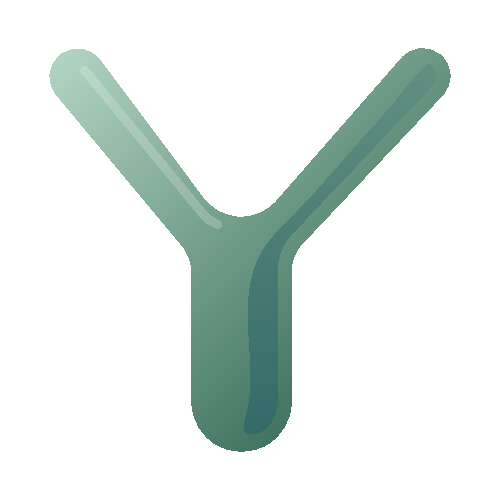
\includegraphics[height=52mm]{figures/yuzen-mark.pdf}

\vspace{14mm}

{\sffamily\bfseries\fontsize{54pt}{58pt}\selectfont\color{yznInk} Yuzen}

\vspace{5mm}

{\sffamily\fontsize{13pt}{18pt}\selectfont\color{yznShadow}
 A thin liquid film flow solver\\ based on the lubrication approximation}

\vspace{9mm}

{\color{yznCeladon}\rule{46mm}{1.2pt}}

\vspace{9mm}

{\sffamily\fontsize{15pt}{19pt}\selectfont\color{yznInk} User Manual}

\vspace{3mm}

{\sffamily\small\color{yznInk!70} Version 1.0 \quad\textbullet\quad \today}

\vspace*{\stretch{3}}

{\sffamily\small\color{yznInk!75}
 Suguru Shiratori\\[2pt]
 Tokyo City University}

\vspace{6mm}
\end{titlepage}

\cleardoublepage
\thispagestyle{empty}
\vspace*{\stretch{1}}
\noindent
{\sffamily\bfseries\large\color{yznShadow} Yuzen User Manual}

\medskip
\noindent
Documents Yuzen version 1.0.

\medskip
\noindent
Copyright \textcopyright{} 2017--2026 Suguru Shiratori, Tokyo City University.

\medskip
\noindent
Yuzen is distributed under the Apache License, Version 2.0. You may obtain a
copy of the license at \url{https://www.apache.org/licenses/LICENSE-2.0}.
See the files \file{LICENSE} and \file{NOTICE} in the distribution.

\medskip
\noindent
Bundled third-party code: doctest (MIT), toml++ (MIT, with one local fix).
Fetched at build time: Eigen (MPL-2.0, required), AMGCL (MIT, optional).
See \file{THIRD\_PARTY\_NOTICES.md}.

\medskip
\noindent
This manual is generated from the sources in \file{docs/manual/} and is built
with Lua\LaTeX. Every number quoted in \cref{ch:verification} is reproducible
from the repository; the commands are given with the number.

\vspace*{\stretch{2}}
\cleardoublepage


\cleardoublepage
\pdfbookmark[0]{Contents}{toc}
\tableofcontents

% preface.tex -- how to read this manual
\chapter*{Preface}
\addcontentsline{toc}{chapter}{Preface}
\markboth{Preface}{Preface}

This manual documents Yuzen, a solver for the flow of a thin liquid film on a
substrate. It is written for several readers, and none of them has to read the
whole of it.

\begin{description}
  \item[To run a calculation,] read \cref{ch:introduction,ch:installation,ch:firstrun},
    then keep \crefrange{ch:inputformat}{ch:output} open beside you: they are
    the reference for every input key and every output file.
  \item[To know what is being solved,] read Part~III: the governing equations,
    what each term and dimensionless group means, and the contact-line model
    (\cref{ch:wetting}, which decides the mesh for any moving contact line).
  \item[If a run is slow or will not converge,] read Part~IV, beginning with
    \cref{ch:convergence}: most slow runs on a fine mesh are its floor of the
    Newton correction meeting an absolute convergence test.
  \item[To modify the solver,] read \cref{ch:reproducibility} first --- the
    results are bit-identical whatever the thread count, and the code that
    makes them so looks untidy and is not --- then \cref{ch:extending},
    \cref{ch:layout} and \cref{ch:policy}.
\end{description}

Part~V reports what has been checked and with what numbers, distinguishing
an analytic solution, a measured order, a conserved invariant and a regression
test; \cref{ch:notverified} lists what has \emph{not} been checked. Keys are
set as \key{Physics.Evaporation.Coef}, values as \val{"WM"}, files as
\file{JobInfo.txt}, code and commands as \code{SetMatrixA()}, environment
variables as \env{YUZEN\_DEBUG\_FLOOR}; all dimensional input is SI, and every
measured number comes with the command that reproduces it.

The name \emph{Yuzen} is written with two Japanese characters: \emph{y\=u},
the glaze on a ceramic, and \emph{zen}, ``as it is, of itself''.

\medskip
\hfill Suguru Shiratori, Tokyo City University


% --- body ------------------------------------------------------------------
\mainmatter

\part{Getting started}
% ch-introduction.tex -- what Yuzen is and what it is for
\chapter{Introduction}
\label{ch:introduction}

Yuzen computes how a thin liquid layer on a substrate evolves in time: how it
levels under surface tension, how it is driven by gravity and rotation, how the
solvent evaporates so that the film thickens and eventually stops flowing, and
how the contact line at its edge advances or recedes.

It is a research solver, written in C++17, with no dependency you have to
install by hand. You describe a case in one text file, run one executable, and
get a directory of results that opens in ParaView.

\section{What Yuzen solves}
\label{sec:intro:what}

Yuzen solves the long-wave (lubrication) equation for the film height
$h(x,y,t)$, coupled to a transport equation for the solute concentration
$c$. In dimensionless form,
%
\begin{align}
  \frac{\partial H}{\partial T} &= -\nabla\cdot\Qvec - \Ev\,\hat{E}(H,C) + \hat{S},
  \label{eq:intro-height}\\
  \frac{\partial (HC)}{\partial T} &= -\nabla\cdot\bigl(C\,\Qvec\bigr)
    + \Df\,\nabla\cdot\bigl(\hat{D}(C)\,H\,\nabla C\bigr) + C_S\,\hat{S},
  \label{eq:intro-conc}
\end{align}
%
where the flux $\Qvec$ collects capillary leveling, disjoining pressure,
vertical and in-plane gravity, centrifugal force and the Marangoni stress.
The first equation moves the liquid; the second moves the solute $HC$ with the
same flux and lets it diffuse, and evaporation, which takes solvent only, is
absent from it --- it concentrates the solute by thinning the film. The liquid
$\hat{S}$ a nozzle supplies brings solute at the concentration $C_S$ it
arrives at: the local $C$ by default, or a concentration of its own. The full
forms are derived in \cref{ch:governing}, each term is discussed in
\cref{ch:terms}, and \cref{ch:concentration} adds a model that resolves $C$
through the thickness.

The approximation behind \cref{eq:intro-height} is that the film is thin
compared with the in-plane length over which it varies. That single assumption
reduces the Navier--Stokes equations to one evolution equation for $h$, which
is what makes it possible to compute a whole coated wafer rather than a few
millimeters of one. It also sets the limits of the model, and
\cref{sec:governing:breakdown} states them explicitly rather than leaving you
to discover them.

\section{Physical processes}
\label{sec:intro:physics}

Each process below is a separate term of the equations, switched on by its
own block of the input file (\cref{ch:ref-physics}); a block left out means
that term is off.

\begin{itemize}
  \item Capillary (Laplace) pressure: leveling by surface tension
    (\cref{sec:terms:laplace}).
  \item Disjoining pressure: wetting, dewetting and a moving contact line on a
    precursor film, calibrated to an equilibrium contact angle
    (\cref{sec:terms:disjoining}, \cref{ch:wetting}).
  \item Vertical gravity, including flow over a non-flat substrate
    (\cref{sec:terms:vgravity}).
  \item In-plane gravity: drainage on an inclined substrate
    (\cref{sec:terms:hgravity}).
  \item Centrifugal force: spin coating (\cref{sec:terms:centrifugal}).
  \item Solutal Marangoni stress (\cref{sec:terms:marangoni}).
  \item Navier slip at the substrate (\cref{sec:terms:slip}).
  \item Solvent evaporation, with spatial profiles and a correction on the
    precursor film (\cref{sec:terms:evaporation}).
  \item Liquid supplied by a fixed or moving nozzle (\cref{sec:terms:source}).
  \item Solute transport, well mixed through the thickness or resolved across
    it, with viscosity, surface tension and diffusivity depending on the
    concentration (\cref{ch:concentration}).
\end{itemize}

\section{What it is good for}
\label{sec:intro:uses}

Typical applications are spin-coated photoresist, functional coatings, drying
films, and wetting and dewetting problems. Concretely, Yuzen is a reasonable
choice when

\begin{itemize}
  \item the film is thin compared with the in-plane features you care about,
        so that $\As = (L_0/h_0)^2$ is large;
  \item the flow is viscous and inertia is negligible;
  \item you need the film shape over seconds to minutes of physical time,
        rather than the three-dimensional velocity field at one instant;
  \item the interesting physics is some combination of leveling, drying,
        Marangoni streaking, spinning and contact-line motion.
\end{itemize}

It is the wrong tool when inertia matters, when the interface slope is large
everywhere rather than only near the contact line, when the film breaks up into
droplets that separate, or when you need the flow inside the film in three
dimensions. \Cref{sec:governing:breakdown} quantifies the first two: the
small-angle substitution used to calibrate the contact angle is in error by
\SI{0.3}{\percent} at \ang{10} and by \SI{23}{\percent} at \ang{90}.

\section{What a result looks like}
\label{sec:intro:gallery}

Every figure in this section was drawn from output the solver actually wrote,
by \file{docs/figures/\bk make\_examples.py}, from the cases shipped in
\file{cases/}. Nothing in them is idealized or redrawn by hand: run the cases
and you get these pictures back.

\begin{figure}[tbp]
  \centering
  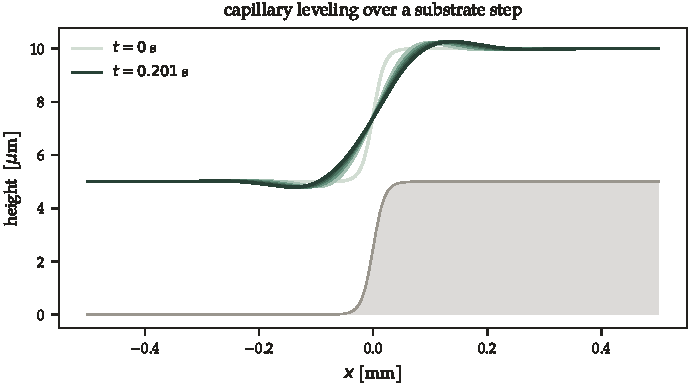
\includegraphics[width=\textwidth]{../figures/leveling-1d.pdf}
  \caption{Capillary leveling over a substrate step, from
    \file{leveling\_1d\_reg.toml}. The gray body is the substrate $s$; the
    curves are the free surface $h+s$ at six times between \SI{0}{\second} and
    \SI{0.2}{\second}, light to dark. The film starts as a layer of uniform
    thickness draped over the step and does not simply flatten: curvature
    drives liquid out of the convex shoulder into the concave foot, so a dip
    opens below the step and a rim builds above it. That pair --- a trough
    before the rise and an overshoot after it --- is the signature of the
    fourth-order leveling operator, and it is what \cref{ch:governing}
    derives.\label{fig:gallery:leveling1d}}
\end{figure}

\begin{figure}[tbp]
  \centering
  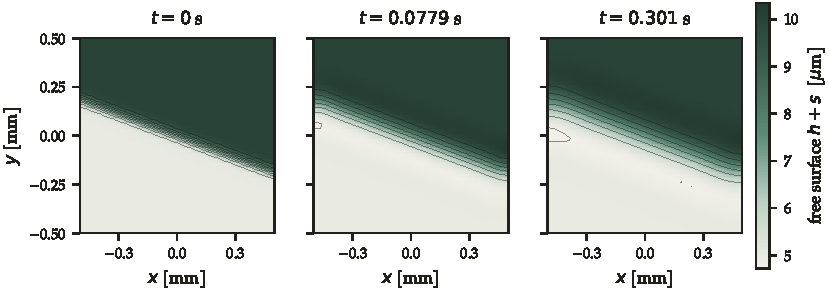
\includegraphics[width=\textwidth]{../figures/leveling-2d.pdf}
  \caption{The same physics in plan view, from \file{allphys\_2d\_reg.toml},
    which has every term switched on, including gravity in the plane and the
    centrifugal term. The color is the free surface $h+s$; the contours are
    drawn from the same field. The initial step is a straight edge crossing the
    domain obliquely, so nothing about the answer is aligned with either grid
    direction, and it spreads into a broad ramp with the trough of
    \cref{fig:gallery:leveling1d} now visible as a closed
    contour.\label{fig:gallery:leveling2d}}
\end{figure}

\section{Models}
\label{sec:intro:models}

Four combinations of dimension and concentration model are implemented. The
choice is made by two keys, \key{Physics.ConcField.Model} and
\key{Grid.Dimension}.

\begin{yzntable}{The four models\label{tab:models}}{@{}L{0.13\textwidth} L{0.13\textwidth} L{0.64\textwidth}@{}}
\textsf{\bfseries Model} & \textsf{\bfseries Dimension} & \textsf{\bfseries Description}\\ \midrule
\val{"WM"} & \val{"xh"}  & 1-D ridge, concentration uniform across the film thickness \\
\val{"WM"} & \val{"xyh"} & 2-D plan view, concentration uniform across the film thickness \\
\val{"CZ"} & \val{"xh"}  & 1-D film, concentration resolved through the thickness, $c(x,z,t)$ \\
\val{"CZ"} & \val{"xyh"} & 2-D film, concentration resolved through the thickness, $c(x,y,z,t)$ (pseudo 3-D) \\
\end{yzntable}

``Well mixed'' means the solute concentration is taken to be uniform across the
film thickness. The \val{"CZ"} model resolves it instead, at the cost of a grid
in $z$ and of two physics terms: disjoining pressure and the source term are
not available there, so contact-line problems must use \val{"WM"}.
\Cref{ch:concentration} compares the two and says when the well-mixed
assumption fails.

\section{How the pieces fit together}
\label{sec:intro:pieces}

A Yuzen run is a single process reading a single input file. \textbf{One
process on one machine} --- Yuzen is parallelized with OpenMP and has no MPI
support, so the size of problem you can solve is bounded by the memory of one
node (\cref{ch:parallel}).

\begin{enumerate}
  \item The input file, a TOML document, is parsed and checked for
        consistency. An inconsistent input aborts the run before any
        computation starts.
  \item The dimensional input is converted to the internal dimensionless form.
        The scales actually used are printed in the run log on standard
        output.
  \item A result directory named after \key{JobName} is created, and the input
        file is copied into it, so a result directory is self-describing.
  \item The solver advances the film height with a Newton--Kantorovich
        iteration, solving the concentration equation inside the same
        iteration, until the end time is reached, the film dries out, or the
        solution goes steady.
  \item Fields, history and per-step diagnostics are written at independent
        intervals.
\end{enumerate}

The height equation is advanced with Crank--Nicolson in time and an analytic
Jacobian assembled term by term; the concentration equation is solved
semi-implicitly inside the Newton loop, so that the converged state satisfies
both equations simultaneously (\cref{sec:time:coupling}). The time step adapts
from a local truncation error estimate. Two linear-solver backends are
available behind one interface, Eigen and AMGCL (\cref{ch:linearsolver}).

\section{Reproducibility}
\label{sec:intro:repro}

Two properties are worth stating at the outset because they shape the code.

First, Yuzen returns \emph{bit-identical} results regardless of OpenMP thread
count, with the \val{"amgcl"} backend as the documented exception. The test
suite asserts this and \code{ctest} re-runs the whole suite under one and four
threads. \Cref{ch:reproducibility} explains the four implementation details
that this depends on --- and why none of them may be ``tidied up''.

Second, every number in \cref{ch:verification} is reproducible from the
repository, and the command that reproduces it is printed next to it.
\Cref{ch:notverified} lists what has not been checked.

\section{License and citation}
\label{sec:intro:license}

This manual documents Yuzen 1.0. \Cref{ch:policy} says what the version number
promises about input files and about results, and \cref{ch:revisions} lists
what this release contains.

Yuzen is distributed under the Apache License, Version 2.0; see \file{LICENSE}
and \file{NOTICE}. Bundled third-party code is doctest (MIT) and toml++ (MIT,
with one local fix); Eigen (MPL-2.0, required) and AMGCL (MIT, optional) are
fetched at build time. \file{THIRD\_PARTY\_NOTICES.md} gives their versions
and describes the change to toml++. If you use Yuzen in published work, please
cite it as given in \file{CITATION.cff}.

The code, its comments, the source documents in \file{docs/} from which
Parts~III to~V of this manual are derived, and this manual itself are all in
English.

% ch-installation.tex -- requirements, build, options, test suite
\chapter{Building Yuzen}
\label{ch:installation}

Yuzen builds with CMake and has no dependency you have to install by hand. If
Eigen is not already present, CMake fetches it; if AMGCL is not present and you
asked for it, CMake fetches that too, and falls back to an Eigen-only build if
it cannot.

\section{Requirements}
\label{sec:install:requirements}

\begin{itemize}
  \item A C++17 compiler. The CI matrix covers GCC, Clang and MSVC on Linux,
        macOS and Windows.
  \item CMake $\ge$ 3.16.
  \item OpenMP, if you want the parallel build (on by default; the serial build
        is fully supported and gives the same numbers). With GCC, install
        LLVM's \code{libomp} as well (\code{apt install libomp-dev}, or the
        \code{libomp} package of a Red Hat system): the build then links it
        instead of GCC's own runtime, and runs on many cores are faster
        (\cref{sec:parallel:runtime}). \textbf{There is no MPI
        dependency and no MPI build}: Yuzen is shared-memory parallel only
        (\cref{ch:parallel}).
  \item Optionally Eigen $\ge$ 3.3 and AMGCL, if you would rather supply them
        yourself than have CMake fetch them. On Debian and Ubuntu that is
        \code{apt install libeigen3-dev}; on macOS, \code{brew install eigen};
        with vcpkg, \code{vcpkg install eigen3}.
\end{itemize}

Fetching happens only when the dependency is missing, so a machine without
network access needs Eigen installed beforehand --- and, if you want it, AMGCL.

\begin{note}[Non-ASCII file names on Windows]
  The solver handles file names as UTF-8, which is what the input file is
  and what Linux and macOS use. An MSVC build embeds a manifest
  (\file{yuzen/src/yuzen.manifest}) that makes UTF-8 the code page of the
  process, so that an input file, a \key{JobName} or a
  \key{Restart.FileName} with Japanese characters names the same file on
  Windows. That needs Windows 10 version 1903 or later; on an older Windows,
  keep those names ASCII. Paths longer than 260 characters need the Windows
  long-path setting as well.
\end{note}

\section{The build}
\label{sec:install:build}

From the top of the repository:

\begin{shell}
cmake -S . -B build -DCMAKE_BUILD_TYPE=Release
cmake --build build -j
ctest --test-dir build
\end{shell}

\code{ctest --test-dir} needs CMake 3.20 or later. An older \code{ctest}
ignores the option, finds no tests and still exits with 0, so with CMake 3.16
to 3.19 run \code{cd build \&\& ctest} instead. The whole suite takes about 25 minutes on two
cores; \code{ctest -R yuzen\_tests} runs the unit tests alone in a few seconds.

This produces two executables in \file{build/bin/}: the solver \file{yuzen} and
the test binary \file{yuzen\_tests}. Run \file{yuzen --version} and it
prints its full version --- \code{Yuzen-1.0.0}, as
\code{MAJOR.MINOR.PATCH}; with no argument it prints its usage. Input
files name only the \code{MAJOR.MINOR} series; \cref{ch:policy} says what that
distinction promises and \cref{ch:revisions} what each release changed. The
build type defaults to \val{Release}
if you do not set it; do not benchmark a \val{Debug} build, and do not draw
conclusions about convergence from one either, since the difference in rounding
is not the interesting kind.

\section{Build options}
\label{sec:install:options}

\begin{yzntable}{CMake options\label{tab:cmake-options}}{@{}L{0.30\textwidth} L{0.10\textwidth} L{0.52\textwidth}@{}}
\textsf{\bfseries Option} & \textsf{\bfseries Default} & \textsf{\bfseries Effect}\\ \midrule
\code{YUZEN\_ENABLE\_OPENMP}   & \val{ON} & OpenMP parallelization. Turning it off also removes the two extra \code{ctest} entries that check thread invariance. \\
\code{YUZEN\_WITH\_AMGCL}      & \val{ON} & Build the AMGCL backend. If the headers cannot be found or fetched, the build warns and continues without it. \\
\code{YUZEN\_STRICT\_WARNINGS} & \val{ON} & \code{-Wall -Wextra} and the implicit-fallthrough warning. \\
\code{YUZEN\_BUILD\_TESTS}     & \val{ON} & Build \file{yuzen\_tests} and register the \code{ctest} entries. \\
\code{YUZEN\_PREFER\_LIBOMP}   & \val{ON} & GCC on Linux: link LLVM's OpenMP runtime \code{libomp} instead of GCC's \code{libgomp} when it is installed; its parallel regions cost a quarter as much on 56 threads (\cref{sec:parallel:runtime}). \\
\code{YUZEN\_OPENMP\_RUNTIME}  & (empty) & The path of an OpenMP runtime to link instead of the compiler's own (\file{libomp.so}, \file{libiomp5.so}); it takes precedence over \code{YUZEN\_PREFER\_LIBOMP}. \\
\end{yzntable}

So, for example, a minimal build without AMGCL and without tests is

\begin{shell}
cmake -S . -B build -DCMAKE_BUILD_TYPE=Release \
      -DYUZEN_WITH_AMGCL=OFF -DYUZEN_BUILD_TESTS=OFF
cmake --build build -j
\end{shell}

Both settings of \code{YUZEN\_WITH\_AMGCL} are supported configurations and
both compile; the \code{\#ifdef} that distinguishes them never appears in a
header, only in \file{yuzen/src/\bk numerics/\bk LinearSolverBackend.cpp}. If you ask
for the \val{"amgcl"} backend in an input file but built without it, the run
warns and falls back to \val{"eigen"} (\cref{sec:linsolve:backends}).

\section{Installing}
\label{sec:install:install}

The solver can be run from \file{build/bin/} as it is. To put it somewhere
else,

\begin{shell}
cmake --install build --prefix $HOME/.local
\end{shell}

copies \file{yuzen} into \file{bin/} under the prefix, and \file{LICENSE},
\file{NOTICE}, \file{THIRD\_PARTY\_NOTICES.md} and \file{README.md} into
\file{share/doc/yuzen/}. Nothing else is installed: Eigen and AMGCL are
header-only and compiled in, and the scripts of \file{tools/}, the cases and
this manual are used from the source tree.

\section{The test suite}
\label{sec:install:tests}

\begin{shell}
ctest --test-dir build
\end{shell}

\code{ctest} registers seventeen entries (sixteen where SymPy is not
installed). Three run the test binary in separate
processes: once with whatever thread count the environment gives, once with
\env{OMP\_NUM\_THREADS=1} and once with \env{OMP\_NUM\_THREADS=4}. That is not
redundancy. Thread invariance is one of the claims the suite makes, and it can
only be asserted across processes (\cref{ch:reproducibility}). Twelve run the
solver itself: \code{concz\_vs\_wm} and \code{concz\_vs\_wm\_2d} check
that the two concentration models agree where they must;
\code{restart\_roundtrip} that a restart of either model, in 1-D and 2-D, from
the \file{.vts} (in \val{"CZ"} also one without the thickness and substrate) and from the \file{field*.dat}, starts from the state and the
time it was given (\cref{sec:ref-numerics:restart}), and that each \file{.vts}, read through the offsets in its header, holds what the field file of the same instant holds; \code{restart\_chain}
that a run stopped and restarted several times, from either format, gives the
same files, bit for bit, as one that ran straight through; \code{input\_guards}
that inputs which would otherwise run with a silently wrong answer --- a misspelled key, a
one-sided \val{"Periodic"}, a \val{"Periodic"} edge on a rotating film, a
pinned edge facing a film of full thickness ---
are refused with the reason; \code{error\_paths} that what a new user, a full
disk or a job scheduler does to a run --- a wrong command line, input file or
result directory, a missing or truncated restart file, a file size limit or a
full device, \code{SIGINT}, \code{SIGTERM} or \code{SIGKILL} in the middle
of a run, paths with spaces and Japanese characters --- stops it with the path
and the reason and leaves no file cut short, and that a run interrupted and
continued is, bit for bit, the run made straight through
(\cref{sec:output:failures}); \code{equivalence} that the same problem
posed in two ways gives the same answer (\cref{sec:verification:equivalence});
\code{analytic} that the problems with a closed-form answer get it, at
the order the scheme promises (\cref{sec:verification:analytic}); \code{mms}
that a manufactured solution with a large amplitude, with every term of each
model on, converges at second order in space and time
(\cref{sec:verification:mms}); \code{advection} that the convection schemes
keep a concentration step within its bounds where they promise to, and
converge on a smooth one at their order, and that the well-mixed
concentration converges in 2-D at second order with convection and
diffusion together (\cref{sec:verification:schemes});
\code{features} that the probes, the
steady-state, dry-out and \key{MaxSteps} stops and the growth of an adaptive
time step do what they say (\cref{sec:verification:features}); and
\code{proptest} that random valid inputs end cleanly, keep the film positive
and the volume and the solute, and are invariant where they must be
(\cref{sec:verification:fuzzing}). One runs no
solver: \code{doc\_keys} reads every key the parser reads, with its type,
default, range and accepted values, holds the key tables of
\cref{ch:ref-domain,ch:ref-physics,ch:ref-bcout,ch:ref-numerics}, the TOML
listings of this manual and every file in \file{cases/} to it, and has the
binary read each case with \code{--check-input}
(\cref{sec:inputformat:unknown}). The last,
\code{mms\_source\_current}, is registered only where SymPy is installed: it
checks that the generated source of the manufactured solution is up to date.
All but the three test-binary entries need a Python interpreter and are left
out without one.

Running the test binary directly prints the counts:

\begin{plain}
$ ./build/bin/yuzen_tests
[doctest] test cases:    128 |    128 passed | 0 failed | 0 skipped
[doctest] assertions: 183297 | 183297 passed | 0 failed |
\end{plain}

These are not smoke tests. They assert against analytic solutions, conservation
laws and convergence orders; \cref{sec:verification:suite} lists what each of
the seventeen test files fixes.

\section{Repository layout}
\label{sec:install:layout}

\begin{plain}
yuzen/src/grid/        structured grid and fields (staggered, type-tagged)
yuzen/src/numerics/    vectors, CRS matrices, linear solvers, time integrators
yuzen/src/model/       the physics: pressure terms, equations, model drivers
yuzen/src/IO/          input parsing, output, restart, probes
yuzen/src/util/        logging, paths, job information
yuzen/src/commonFunctions/   shape functions and shape generation
yuzen/tests/           the test suite
cases/                 example and regression input files
tools/                 helper scripts
docs/                  theory, numerics, validation, and this manual
third_party/           doctest, toml++
\end{plain}

\Cref{ch:layout} goes through this in more detail, for readers who intend to
modify the solver.

\section{Continuous integration}
\label{sec:install:ci}

\file{.github/workflows/ci.yml} builds and tests on Ubuntu with GCC and Clang
(and with GCC 11, the system compiler of RHEL 9 and of many clusters),
on Windows with MSVC, and on macOS with Clang, all \emph{without} AMGCL so
that the plain configuration is the one kept honest, and once more on Ubuntu
with GCC and AMGCL, so that the code path taken only with AMGCL is built and
tested too.

\section{If the build fails}
\label{sec:install:trouble}

\begin{description}
  \item[Eigen is fetched every time.] CMake only fetches when
    \code{find\_package(Eigen3 3.3 QUIET NO\_MODULE)} fails. Install Eigen
    system-wide, or point \code{Eigen3\_DIR} at it, and the fetch stops.
  \item[AMGCL cannot be fetched.] The build warns, sets
    \code{YUZEN\_WITH\_AMGCL} to \val{OFF} and continues. Nothing else is lost;
    you simply have one backend, \val{"eigen"}, instead of two.
  \item[OpenMP not found on macOS.] Apple Clang needs \code{libomp}
    (\code{brew install libomp}). If you would rather not, configure with
    \code{-DYUZEN\_ENABLE\_OPENMP=OFF}: the serial build produces exactly the
    same numbers.
  \item[Warnings you do not want.] Configure with
    \code{-DYUZEN\_STRICT\_WARNINGS=OFF}. Please do not make this the default
    for development work; the warning set was turned on deliberately.
\end{description}

% ch-firstrun.tex -- the first calculation, start to finish
\chapter{Your first calculation}
\label{ch:firstrun}

This chapter runs one case from beginning to end, looks at what came out, and
then changes one thing at a time so that you can see which part of the input
file controls which part of the answer. It assumes you have built Yuzen as in
\cref{ch:installation}.

\section{Running a case}
\label{sec:firstrun:run}

A run takes one argument, the input file:

\begin{shell}
cd <repository root>
mkdir -p run1 && cd run1
../build/bin/yuzen ../cases/tutorial_1d.toml
\end{shell}

The input file may be given by any path, relative or absolute, with spaces or
non-ASCII characters in it. Besides it the solver knows three options:
\code{--check-input FILE} reads and checks the file and runs nothing
(\cref{sec:inputformat:unknown}), \code{--help} prints the usage and
\code{--version} the version. Anything else --- no argument, two input files,
an unknown option --- prints the usage on standard error and ends with exit
code 1, as does an input file that is missing, a directory or unreadable.
\Cref{tab:exitcodes} lists the exit codes.

It prints a banner, the version and the OpenMP thread count, reads the input,
checks it for consistency, creates the result directory and starts stepping.
The result directory is named after the \key{JobName} key in the input file ---
not after the input file --- so this run produces \file{tutorial\_1d/}. Every
case under \file{cases/} sets \key{JobName} to its own file name, so the
result directory is named after the case it came from.

\begin{note}[Run in a scratch directory]
  Output is written relative to the working directory, so run from wherever you
  want the results. \file{tools/run\_case.sh} does exactly that, and fixes the
  thread count and keeps the log as well (\cref{sec:env:tools}):
  \begin{shell}
./tools/run_case.sh cases/leveling_1d_reg.toml runs/reg 1
  \end{shell}
\end{note}

The case used here, \file{cases/tutorial\_1d.toml}, is a 1-D well-mixed film:
\SI{1}{\milli\metre} wide, \SI{300}{} cells, a \SI{10}{\micro\metre} height
scale, capillary leveling and Marangoni stress on, evaporation on, running to
\SI{0.5}{\second}. It takes a few seconds.

\section{What came out}
\label{sec:firstrun:output}

\begin{plain}
tutorial_1d/
  tutorial_1d.toml        a copy of the input, so the directory is self-describing
  JobInfo.txt             version, machine, linear-solver backends, start and end time
  Warnings.txt            warnings; zero-length if there were none
  FatalErrors.txt         why the run aborted; zero-length if it did not
  field00000.dat ...      the field, as tab-separated text (also the restart format)
  field00000.vts ...      the same field as VTK structured grid
  field00000.state ...    what a restart needs beyond the field (time, step, totals)
  tutorial_1d.pvd         ParaView time series pointing at the .vts files
  History.dat             volume, mean concentration, extrema, conservation error
  CalcInfo.dat            per-output-interval solver diagnostics
\end{plain}

The terminal and the text files at the top of the listing are worth reading
first, in this order.

\paragraph{The terminal} carries the run log: it goes to standard output and is
not written to any file in the result directory. What you saw scroll past opens
with what the solver built from your input --- the linear-solver backend and
the convection scheme of each equation, the grid, the scales used to non-dimensionalize the
problem ($L_0$, $H_0$, $T_0$, $U_0$, under \code{Scaling factors}) and the
dimensionless groups derived from them, the model --- and then becomes the
progress log. A
dot is one time step, \code{dt+} and \code{dt-} mark the adaptive step growing
and shrinking, and \code{Field file $n$, Time = $\dots$} marks each field
written. The run ends with the termination message, and it is the first thing
to check:

\begin{plain}
############## Time reached to the EndTime. #############
Field file 5, Time = 1.606806e-05
Largest Courant number of Numerics.Convection.Height = "Koren": 0.000469

############## Program normally terminated. #############
\end{plain}

There are three normal endings --- \code{Time reached to the EndTime.},
\code{Dry out.} and \code{Steady state.} --- and they mean quite different
things about your case. \Cref{sec:convergence:termination} explains each, and
in particular why a run that reports \code{Steady state.} after a dozen steps is
usually telling you something about the criterion rather than about the physics.

To keep the log, redirect it yourself --- \code{yuzen case.toml > run.log} ---
or use \file{tools/run\_case.sh}, which does the redirection for you and leaves
everything the terminal would have shown in \file{stdout.txt} in the run
directory.

To stop a run early, press Ctrl-C once: the step in progress finishes, the
state reached is written as a field file with its \file{.state}, and the run
ends with \code{Program stopped by SIGINT; its output is complete.} That file
can be restarted from (\cref{sec:firstrun:restart}) and the continued run is
the one that was not stopped, to the bit. A second Ctrl-C ends the process at
once. \Cref{sec:output:failures} has the details, and what happens on a full
disk.

\paragraph{\file{JobInfo.txt}} records the version, the compiler, the machine,
the start and end times, and one section derived from your input: the model and
the linear-solver backend that each equation actually used
(\cref{sec:output:jobinfo}). If a result looks wrong by orders of magnitude,
the scales to check --- $L_0$, $T_0$ and $U_0$ --- are in the run log, not here
(\cref{sec:governing:scales}).

\paragraph{\file{Warnings.txt}} always exists and carries no banner, so it is
\textbf{zero-length exactly when no warning was raised}. Anything in it is a
real message.

\paragraph{\file{FatalErrors.txt}} exists too, and is likewise zero-length
unless the run aborted. When it does abort, the reason is written here
\emph{and} to standard error, so the message is in the result directory and on
the terminal at once. The one case with no file to read is an input the solver
rejects: that happens before the result directory is made, so the message is on
standard error only (\cref{sec:output:warnings}).

\section{Reading the field files}
\label{sec:firstrun:fields}

\file{field00000.dat} is tab-separated text with a one-line header. In 1-D:

\begin{plain}
xx[mm]  HS[um]  Ux[m/s]  CC[-]  HH[um]  SS[um]
-5.00000000000000111e-01  5.00000000000000000e+00  0.0 ...
\end{plain}

\begin{yzntable}{Columns of \file{field*.dat}\label{tab:fieldcols}}{@{}L{0.09\textwidth} L{0.13\textwidth} L{0.70\textwidth}@{}}
\textsf{\bfseries 1-D} & \textsf{\bfseries 2-D} & \textsf{\bfseries Meaning}\\ \midrule
\code{xx} & \code{xx}, \code{yy} & in-plane coordinate, in \si{\milli\metre} \\
\code{HS} & \code{HS}            & free-surface height, $h + s$, in \si{\micro\metre} \\
\code{Ux} & \code{Ux}, \code{Uy} & in-plane velocity, the mixed velocity of all active terms, in \si{\metre\per\second} \\
\code{CC} & \code{CC}            & solute concentration, a mass fraction \\
\code{HH} & \code{HH}            & film thickness $h$, in \si{\micro\metre} \\
\code{SS} & \code{SS}            & substrate height $s$, in \si{\micro\metre} \\
\end{yzntable}

The units above are what you get with \key{Output.Dimensioned} at its default
\val{true}; with \val{false} every column is non-dimensional. Note that the
in-plane and out-of-plane lengths are \emph{not} in the same unit, which is why
the sample line above reads $-0.5$ for a point \SI{0.5}{\milli\metre} from the
center and $5.0$ for a film \SI{5}{\micro\metre} thick.

\begin{warn}[\code{HS} is the free surface, \code{HH} is the thickness]
  The second column is $h+s$, not $h$. \Cref{fig:film-geometry} shows which is
  which. The concentration is the fourth column, not the last one.
\end{warn}

\begin{figure}[tbp]
  \centering
  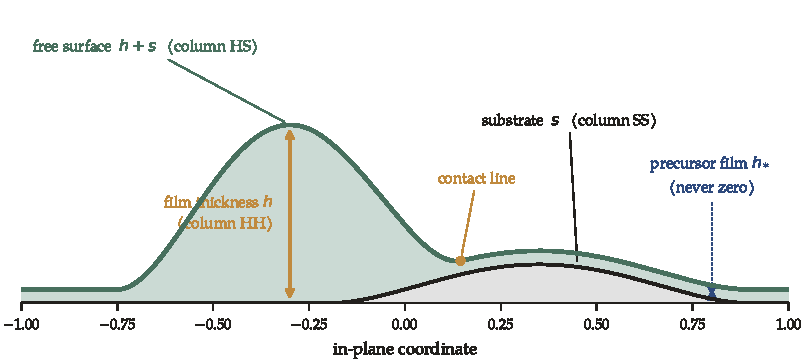
\includegraphics[width=\textwidth]{figures/film-geometry.pdf}
  \caption{The three height columns of \file{field*.dat}, on a droplet sitting
    on a precursor film over a substrate feature. \code{SS} is the substrate
    $s$, \code{HS} is the free surface $h+s$ --- the profile you would see ---
    and \code{HH} is the film thickness $h$ between them. Over a flat substrate
    \code{HS} and \code{HH} coincide and the distinction is invisible; over
    topography they are the difference between the surface you would see and
    the layer of liquid there is. The precursor film $h_*$, set by
    \key{Initial.\bk SurfaceShape.\bk PrecursorRatio}, is the floor below which
    \code{HH} never falls, so the contact line is where the free surface meets
    it rather than a point of zero thickness (\cref{ch:wetting}).
    \label{fig:film-geometry}}
\end{figure}

Whether these numbers are dimensional or dimensionless is set by
\key{Output.Dimensioned}. The values are written with 18 significant digits
regardless, because this same file is the ASCII restart format: at the default
six digits, passing the height through a second difference (dividing by
$\Delta x^2$) corrupts the pressure --- on a contact-line mesh with $\Delta x =
\SI{0.3}{\micro\metre}$, output precision alone shifted the pressure by a few
percent and the velocity derived from it by three orders of magnitude.

For a quick look at the shape, any plotting tool will do:

\begin{shell}
gnuplot -p -e 'plot "tutorial_1d/field00004.dat" u 1:2 w l title "free surface"'
\end{shell}

\section{Viewing in ParaView}
\label{sec:firstrun:paraview}

Open \file{tutorial\_1d/tutorial\_1d.pvd}. It is a collection pointing at the
\file{.vts} files with their time stamps, so ParaView gets the whole time
series with the correct times in one step --- not a numbered sequence it has to
guess at. Set
\key{Output.FieldData.VTKFile} to \val{false} if you do not want the VTK files
at all; \key{NeutralFile} controls the text ones independently.

\section{Changing one thing at a time}
\label{sec:firstrun:changing}

Copy the case and edit it. The following changes are, in rough order, the ones
worth making first.

\paragraph{Run longer or shorter.} \key{Numerics.EndTime}, in seconds. Note
that it defaults to \val{0}, which stops the run after a single step rather
than meaning ``no limit'' --- so always set it.

\paragraph{Write more often.} \key{Output.\bk FieldData.\bk TimeInterval} governs the
fields, \key{Output.\bk GeneralHistory.\bk TimeInterval} the scalar history and
\key{Output.\bk CalcInfo.\bk TimeInterval} the solver diagnostics. They are independent;
history and diagnostics are cheap, so it is normal to write them ten to a
hundred times more often than the fields.

\paragraph{Refine the mesh.} \key{Grid.Nx}, counting interior cells only.
Refinement is not free in an unobvious way: the Newton correction cannot fall
below a floor, and the part of it that comes from terms formed as a product
with their matrix entries grows with the step and as the mesh is refined
(\cref{sec:convergence:floor}). If a refined case suddenly becomes very slow,
read \cref{sec:convergence:absolute} before changing anything else.

\paragraph{Turn a physics term on or off.} Every term under \key{Physics} has
its own \key{Enable}. In \file{tutorial\bk\_1d.toml}, vertical gravity,
in-plane gravity, the centrifugal term and the source are off, and
\file{cases/\bk allphys\_1d\_reg.toml} is the same case with everything on.

\paragraph{Make it dry.} \key{Physics.Evaporation.Coef} sets the evaporation
velocity in \si{\metre\per\second}; it feeds both $\Ev$ and $\Pen$. Watch
\code{AveC} in \file{History.dat} rise as the solvent leaves. With the
viscosity exponent at 10, as in this case, a concentration change of 0.1
multiplies the viscosity by $e$, and the film visibly stops flowing --- that
coupling is the most strongly non-linear thing in the solver
(\cref{sec:conc:properties}).

\paragraph{Add a contact line.} Enable \key{Physics.DisjoiningPressure} and set
\key{ContactAngle}, \key{ExponentN}, \key{ExponentM} and
\key{Initial.SurfaceShape.PrecursorRatio}. Do not do this without reading
\cref{sec:wetting:sizing} first: the mesh and the droplet height are not free
choices once you have named a contact angle, and a case that violates the two
sizing rules produces an answer that looks plausible and has the wrong angle in
it.

\section{Restarting}
\label{sec:firstrun:restart}

Because \file{field*.dat} is also the restart format, any output can be a
starting point. Point \key{Restart} at the file and enable it:

\begin{toml}
[Restart]
Enable      = true
ASCII       = true
FileName    = "tutorial_1d/field00005.dat"
RestartTime = 0.501237
FileIndex   = 6
\end{toml}

and raise \key{Numerics.EndTime}, which is absolute, past \key{RestartTime}.
\key{RestartTime} is the time of that file as \file{tutorial\_1d.pvd} lists
it: a field is written at the step nearest its scheduled time, not exactly on
it. Given that time, the run reads \file{field00005.state} beside the field
file as well and continues exactly as the uninterrupted run would have
(\cref{sec:ref-numerics:restart}); the run log says
\code{continuing exactly from tutorial\_1d/field00005.state}. Given another
time, it takes the field alone and says so.

\key{FileName} is resolved relative to the \textbf{working directory you launch
the solver from}, not relative to the result directory. The file written by the
run above landed in \file{tutorial\_1d/}, so from the same directory you ran in,
the path has to carry that prefix; a bare \file{field00005.dat} would only work
if you ran from inside \file{tutorial\_1d/} --- which would also be where the
new run tried to write its own results.

The shape in \key{Initial.SurfaceShape} is then read but not used. This is also
how an analytically constructed initial state gets in: \file{cases/eq/} and
the \file{cases/wet\_*.toml} cases start from equilibrium droplets built by
\file{tools/make\_equilibrium\_1d.py}, precisely so that the run does not begin
with a spurious velocity at the contact line. \Cref{ch:ref-numerics} documents
the keys and \cref{sec:wetting:equilibrium} the construction.

\section{Comparing two runs}
\label{sec:firstrun:compare}

\begin{shell}
./tools/run_case.sh cases/leveling_1d_reg.toml runs/reg_th1 1
./tools/run_case.sh cases/leveling_1d_reg.toml runs/reg_th2 2
python3 tools/compare.py runs/reg_th1 runs/reg_th2
\end{shell}

\file{tools/compare.py} reports, column by column, the largest difference
divided by the scale of that column, in \file{History.dat}, in
\file{CalcInfo.dat} and in the final \file{field*.dat}. For a pair of runs that
differ only in thread count the answer is \code{0.000e+00}, exactly, and this
is asserted rather than hoped for (\cref{sec:verification:linalg}). It is the
right tool to reach for after changing the solver: if the number is not zero,
you changed the numerics, not just the code.

The four solver-diagnostic columns of \file{CalcInfo.dat} --- \code{NK\_iter},
\code{NK\_resid}, \code{BCG\_iter} and \code{BCG\_resid} --- are held out of
that verdict and, when they differ, reported separately on the line of
\file{CalcInfo.dat}, as the largest
difference-over-column-scale among them. They say how the answer was reached
rather than what it is, so they may legitimately move; do not read that second
number as a total iteration count.


\part{Using Yuzen}
% ch-inputformat.tex -- the input file: TOML, type conversion, map of the blocks
\chapter{The input file}
\label{ch:inputformat}

A Yuzen run is described by exactly one text file, which you pass to the
executable on the command line. That file is a \textbf{TOML} document. This
chapter explains how Yuzen uses TOML: how the block structure of a case maps
onto TOML tables, how a written value becomes a number inside the solver, how
defaults and required keys are expressed, and which mistakes the reader will
\emph{not} tell you about. The keys themselves are documented block by block in
\cref{ch:ref-domain,ch:ref-physics,ch:ref-bcout,ch:ref-numerics}; the map in
\cref{sec:inputformat:map} tells you which of those chapters to open.

Read this chapter once before you write your first input file by hand. Most of
the ways a Yuzen run goes wrong quietly --- rather than aborting with a message
--- are properties of the reader described here, not of the physics.

\section{TOML, chosen by the file name}
\label{sec:inputformat:formats}

The reader layer is \code{yuzen::config::Block}, and it picks the parser from
the file-name extension alone. A name ending in \file{.toml} is parsed with
toml\texttt{++}; that is the format this manual specifies, and the one to write
new work in. Nothing inside the file influences the choice, so renaming a TOML
file to something else does not convert it --- it hands the file to the \file{.inp}
parser of \cref{sec:inputformat:legacy}, which then fails on TOML syntax.

TOML itself is a published standard and is not re-specified here. Its grammar
--- comments, strings, numbers, booleans, arrays, tables --- is at
\url{https://toml.io}, and any TOML parser, editor mode or scripting library
will read a Yuzen input file correctly. What is specific to Yuzen, and what the
rest of this chapter documents, is which TOML constructs the solver's block
tree is built from, and what happens to a value on its way from the file into a
variable.

\section{Blocks are tables}
\label{sec:inputformat:tables}

A Yuzen case is a tree: named blocks, nested inside one another, each holding
keys and further blocks. That tree maps onto TOML in four steps.

\begin{description}
  \item[A block is a table.] \key{Grid} is written \code{[Grid]}, and every
    key after that header up to the next header belongs to it.
  \item[A nested block is a dotted table path.] \key{Evaporation} inside
    \key{Physics} is \code{[Physics.Evaporation]}; \key{SurfaceShape} inside
    \key{Initial} is \code{[Initial.SurfaceShape]}. The depth is not limited,
    and a container that carries no keys of its own ---
    \code{[Initial]}, \code{[Physics]} --- may be written as an empty table
    or left out entirely, since the dotted header of a child creates it.
  \item[A repeated block is an array of tables.] Write the header in double
    brackets, \code{[[Substrate.EllipseBump]]}, once per occurrence;
    \cref{sec:inputformat:repeat} says which blocks may repeat.
  \item[A vector-valued key is an array.] \code{Center = [0.5, 0.0]}. The two
    components are the $x$ and $y$ values, in that order, in 1-D runs as well.
\end{description}

Keys written before the first table header are the \textbf{root-level} keys:
\key{SolverName} and \key{JobName}, and the optional length-scale pair. TOML
requires them to come first, before any \code{[...]} line, because everything
after a header belongs to that table. A \key{JobName} placed after
\code{[Grid]} is a key of \key{Grid}, and the run stops for want of a
root-level \key{JobName}.

Block names, key names and string values are \textbf{case-sensitive}:
\key{Nx} is the grid size, and \code{nx} is an unknown key that stops the run
(\cref{sec:inputformat:unknown}). A string value that differs from an accepted
one only in case, such as \val{"ilu"} for \val{"ILU"}, is refused too, and the
message names the spelling that would have been accepted.

Key names are written in \code{PascalCase} (\key{NewtonMaxIterations},
\key{EndConcValue}), with American spelling (\key{Center}).

\section{How a written value becomes a number}
\label{sec:inputformat:types}

Conversion happens at read time and is decided by the type of the destination
variable in the solver, not by the TOML type you wrote. toml\texttt{++} hands
every scalar to \code{yuzen::config::Block} as text, and the text is converted
when the solver asks for the key. Writing \val{Nx = 300.0} is therefore legal,
and so is \val{Enable = 1}. The four conversions are strict: a value is converted whole or refused, and
the refusal names the key path and the value.

\begin{description}
  \item[bool] True for \val{true}, \val{yes}, \val{on}, \val{1} and
    \val{.true.}; false for \val{false}, \val{no}, \val{off}, \val{0} and
    \val{.false.}, compared case-insensitively. Anything else is refused.
  \item[int] Parsed as a double, which must be a whole number: \val{1e3} is
    1000, \val{1000.4} is refused. A whole number beyond the range of the
    key's integer type --- 32 bits, and 64 for \key{Numerics.MaxSteps} --- is
    clamped to its end.
  \item[double] Parsed with \code{strtod}; the whole text must be the number,
    and \val{nan} and \val{inf} are refused.
  \item[array] Converted element by element with the rules above. A list
    where one value is expected, a nested list or a TOML date or time is
    refused; so is nesting deeper than 64 levels.
\end{description}

The reader imposes no size on an array. Where a key is documented as an array
of two doubles, it is \file{Input.cpp} that checks the length afterwards and
aborts the run if it is not exactly~2. Beyond the conversion, values with
which the equations mean nothing --- a density, viscosity or surface tension
that is not positive, a time step, tolerance or output interval that is not
positive, a negative \key{EndTime}, an initial film with no liquid in it ---
are refused with \code{Input mismatch: key = value: why}; the reference
chapters give the ranges.

\begin{note}[What TOML catches for you]
  A number TOML cannot parse --- \val{1,0e-6} with a comma, \val{1e--6},
  \val{.5} without its leading zero --- is a \emph{syntax error}, and the run
  stops with the file name, the line and toml\texttt{++}'s description of the
  problem. The same goes for an unquoted string: \key{Dimension = xh} is not a
  value at all, where \key{Dimension = "xh"} is. A quoted value in a numeric
  key, such as \key{InitialDt = "fast"}, is valid TOML and is refused by the
  conversion above. Without strict conversions, \key{Enable =
  "ture"} would mean false, an unreadable double would become 0 and a date
  would be dropped as though the key had not been written;
  \file{tools/proptest.py} and the fuzzing of
  \cref{sec:verification:fuzzing} found these during development.
\end{note}

\section{Defaults, required keys and what is missing}
\label{sec:inputformat:defaults}

Whether a key is required is not declared anywhere in the file; it follows
from which overload of \code{getin} the solver calls for it.
\code{getin(name, v)}, with no default, throws \code{VariableNotFound}, which
\code{Input::Read} catches and turns into immediate termination of the
process. \code{getin(name, v, def)} stores \code{def} without a word. Blocks
work the same way: a block fetched with a bare \code{getBlockSize} or
\code{getBlock} is required, one fetched inside a
\code{try \dots{} catch(BlockNotFound)} is optional.

Thirteen keys are required outright across the whole file. They are \key{SolverName}
and \key{JobName} at root level, \key{Dimension}, \key{Nx}, \key{Xmin} and
\key{Xmax} in \key{Grid}, \key{Value} in \key{Initial.Concentration},
\key{Model} in \key{Physics.ConcField} (only when that block is present),
\key{InitialDt} in \key{Numerics}, \key{X} in every
\key{Output.ProbeList.Probe}, and \key{Start}, \key{End} and \key{PerDecade}
in \key{Output.FieldData.LogSchedule} (only when that block is present). Everything else has a built-in default. In the
reference chapters a required key is marked \reqd{} in the default column.

An optional block that is left out reads as an empty one: each of its keys
takes its default. The exceptions are in \key{Physics}: a missing sub-block
there is a term switched off, even where \key{Enable} defaults to
\val{true} inside a block that is written, and a missing
\key{Physics.ConcField} means \key{Model}~$=$~\val{"None"}
(\cref{ch:ref-physics}).

A required \emph{block} that appears twice is just as fatal as one that is
missing: the reader aborts with \code{Block [...] is required and must appear
exactly once}. In TOML
you cannot write a plain table header twice --- \code{[Grid]} twice is a
duplicate-key syntax error that toml\texttt{++} rejects --- so the way to trip
this is to write \code{[[Grid]]}, an array of tables, where a single table
belongs. The chapters that follow say for every block whether it is required
and whether it may repeat, and \cref{tab:file-map} summarizes it for the top
level.

\section{Entries the solver does not know stop the run}
\label{sec:inputformat:unknown}

Every key and every block the reader asks for is recorded, found or not. Once
the whole input has been read, anything in the file that nobody asked for is
something this version does not know --- a misspelled key, a key in the wrong
table, a table with a misspelled name --- and the run stops before anything is
computed, listing each one with its full path:

\begin{plain}
Error in the input: case.toml contains 3 entries that this version of Yuzen
does not read, so whatever they were meant to set would keep its default:
  key   Initial.PrecursorRatio   (this key is read in [Initial.SurfaceShape])
  key   Initial.SurfaceShape.EdgeBump.alpha   (did you mean Initial.SurfaceShape.EdgeBump.Alpha?)
  block [Physics.Evaporaton]   (did you mean [Physics.Evaporation]?)
Correct the spelling or remove the entry. The manual's input reference lists
every key each block accepts.
\end{plain}

A near miss of a name the block does read is offered as the likely intent; a
correctly spelled key in the wrong table is pointed at the table that reads it.
Like the other input errors, this one goes to standard error, before the result
directory exists (\cref{sec:output:running}).

To make these checks without running anything, give \code{--check-input}
before the file name:

\begin{shell}
yuzen --check-input case.toml
\end{shell}

The file is read and checked exactly as for a run --- unknown entries,
required keys, ranges, accepted values and the consistency checks between
keys --- and the program then prints \code{Input check passed} and exits
with status 0, or stops with the reason and status 1. Nothing is created.
A \key{Restart.FileName} that is not there, relative to the directory the
check is made in, is noted in a line starting \code{Note:} but does not fail
the check: the run that reads it may start elsewhere. A run started where it
is missing stops before making its result directory.

Without this, each of those entries would have been read by nobody and the
setting it was meant to change would have kept its default without a word:
the precursor at \val{0}, $\alpha$ at \val{1}, evaporation off. That is why
the check refuses rather than warns.

TOML's own checks are about syntax. A well-formed document with a key in the
wrong place is still well formed, which is why the check above is the solver's
and not toml\texttt{++}'s. What it cannot catch is a correctly spelled key, in
the right table, with the wrong value; for that, read back what the solver
understood --- the grid, the scales and the dimensionless groups it prints to
\textbf{standard output} (\cref{sec:output:running}).

\section{Repeated blocks}
\label{sec:inputformat:repeat}

Some blocks may appear more than once. These are the thirteen shape blocks,
seven under \key{Initial.SurfaceShape} and six under \key{Substrate}, together
with \key{Output.ProbeList.Probe}. The parser sizes the vector from
\code{getBlockSize} and fills it in file order, so four \key{EllipseBump}
blocks build four bumps. Zero copies are allowed as well --- a
\key{Substrate} table with no shape block in it is a flat substrate.

Write each occurrence as an array-of-tables header:

\begin{toml}
[[Substrate.RectBump]]
Order  = 1
Center = [0.0, 0.0]

[[Substrate.RectBump]]
Order  = 2
Center = [1.0e-3, 0.0]
\end{toml}

A block that may appear only once is a plain table, \code{[Substrate]}. The
shipped cases write a \emph{single} occurrence of a repeatable block as a plain
table too --- \code{[Substrate.EllipseBump]} --- and the solver reads it as a
list of one. Both spellings are accepted; use the double-bracket form as soon
as there is more than one, because a second plain \code{[Substrate.RectBump]}
header is a duplicate-key error rather than a second bump.

\section{Units}
\label{sec:inputformat:units}

\textbf{All dimensional input is SI}: meters, seconds, kilograms, \si{\pascal\second},
\si{\newton\per\metre}, \si{\metre\squared\per\second} and radians, except
where a table in the reference chapters says otherwise. Two exceptions are
worth memorizing now. The first is the contact angle,
\key{Physics.DisjoiningPressure.ContactAngle},
which is in \emph{degrees} --- and it is the only angle in the file that is;
the tilt of a \key{FlatPlane} shape, like everything else, is in radians. The
second is \key{Fluid.MolarMass}, which takes any consistent unit, because only
the ratio of its two values is ever used.

You never write a non-dimensional quantity, except for the handful of keys
that are genuinely dimensionless (exponents, ratios, switches and the
tolerances in \key{Numerics}). \code{NonDimensionalNumbers::Build} converts
your SI values into the solver's internal scales and prints the result to
standard output (\cref{sec:output:running}).

\section{A complete fragment}
\label{sec:inputformat:example}

\begin{toml}
# a 1-D film, 1 mm wide
SolverName = "Yuzen-1.0"
JobName    = "demo"

[Grid]
Dimension = "xh"
Nx        = 300
Xmin      = -0.5e-3
Xmax      = 0.5e-3

[Initial.Concentration]
Value = 0.5

[Initial.SurfaceShape]
TotalHeight    = 10e-6
PrecursorRatio = 0.02

[[Initial.SurfaceShape.EllipseBump]]
CreateType = "add"
Height     = 0.5
Center     = [0.0, 0.0]
Width      = [0.4e-3, 1.0]
SlopeWidth = 0.05

[Boundary.XminBC]
Type = "Symmetry"

[Boundary.XmaxBC]
Type = "Outlet"
\end{toml}

This fragment is not a complete input file: \key{Fluid}, \key{Physics},
\key{Output} and \key{Numerics} are required as well, and the run would abort
without them. Note that \code{[Initial]} and \code{[Boundary]} never appear as
headers of their own --- the dotted paths below them create both --- and that
the two root-level keys stand at the top, before any header.

\section{A map of the file}
\label{sec:inputformat:map}

\Cref{tab:file-map} lists everything that may appear at the top level of an
input file, and where in this part of the manual to find its keys. The
version covered throughout is Yuzen 1.0: 58 block paths, 54 of which carry
keys, and 229 key entries in total.

\begin{yzntable}{Every top-level block, and where it is documented\label{tab:file-map}}{@{}L{0.20\textwidth} L{0.13\textwidth} L{0.11\textwidth} L{0.44\textwidth}@{}}
\textsf{\bfseries Block} & \textsf{\bfseries Required} & \textsf{\bfseries Repeats} &
\textsf{\bfseries Contents, and where to read about it} \\ \midrule
Root level & partly & \dash & Keys before the first table header: \key{SolverName} and \key{JobName} are required, the length scale is optional. \Cref{sec:ref-domain:root}. \\
\key{Grid} & yes & no & Dimension, cell counts and domain bounds. \Cref{sec:ref-domain:grid}. \\
\key{Initial} & yes & no & Initial concentration and film shape, with repeatable shape sub-blocks. \Cref{sec:ref-domain:initial}. \\
\key{Substrate} & no & no & Substrate topography, with the same shape sub-blocks. \Cref{sec:ref-domain:substrate}. \\
\key{Fluid} & yes & no & Density, surface tension, viscosity, diffusivity, molar mass. \Cref{sec:ref-domain:fluid}. \\
\key{Physics} & yes & no & Which terms are active and their parameters. \Cref{ch:ref-physics}. \\
\key{Boundary} & yes & no & One condition per domain edge. \Cref{sec:ref-bcout:boundary}. \\
\key{Output} & yes & no & What is written and how often. \Cref{sec:ref-bcout:output}. \\
\key{Numerics} & yes & no & Time stepping, Newton and linear-solver settings. \Cref{sec:ref-numerics:numerics}. \\
\key{Restart} & no & no & Continue from a previous result. \Cref{sec:ref-numerics:restart}. \\
\end{yzntable}

No top-level block may be repeated; a second copy of a required one aborts the
run. The blocks that may repeat are all nested: the seven shape blocks of
\key{Initial.SurfaceShape}, the six of \key{Substrate}, and
\key{Output.ProbeList.Probe}.

\section{The \file{.inp} format}
\label{sec:inputformat:legacy}

Yuzen also reads a block-structured \file{.inp} format: any file name that
does not end in \file{.toml} goes to that parser. \textbf{The format is not
specified in this manual.} It is an alternative input format, and it is not
where new work belongs.

The shipped cases and every example in this manual are TOML.

% ch-ref-domain.tex -- reference: root keys, Grid, Initial, Substrate, Fluid
\chapter{Grid, initial state, substrate and fluid}
\label{ch:ref-domain}

This chapter documents the four blocks that describe \emph{what} is being
computed: the mesh and the domain (\key{Grid}), the state the run starts from
(\key{Initial}), the shape of the solid underneath the film
(\key{Substrate}), and the liquid's material properties (\key{Fluid}). It also
covers the handful of keys that live at root level, outside any block. The
physics terms, the boundary conditions and the numerical settings are in
\cref{ch:ref-physics,ch:ref-bcout,ch:ref-numerics}.

Every default, type and range quoted here is the one the parser actually
applies. Where a key is marked \reqd{}, omitting it terminates the run. A
range written as \emph{range $[a:b]$}, or a bound written as \emph{at least},
is checked when the file is read, and a value outside it stops the run; words
such as \emph{positive} or \emph{non-zero} say what makes sense and are not
checked. These tables are held to the parser by \file{tools/doc\_keys.py},
which \code{ctest} runs (\code{doc\_keys}).

\section{Root level}
\label{sec:ref-domain:root}

Keys written at the top of the file, before the first table header, identify
the run and choose the horizontal length scale. \key{SolverName} is a version gate,
not a solver selector: the model is chosen by \key{Physics.ConcField.Model}
together with \key{Grid.Dimension}. \key{JobName} names the result directory
created next to the run; the input file is copied into it and the ParaView
index file is named after it.

\begin{keytable}{Keys at root level\label{tab:root-keys}}\key{SolverName} & string & \reqd & Solver and input-format stamp. Must be exactly \val{"Yuzen-1.0"}; any other string aborts the run. It names the \code{MAJOR.MINOR} series only, so a patch release does not change it (\cref{ch:policy}). \\
\key{JobName} & string & \reqd & Name of the result directory. Any string. \\
\key{LengthScaleType} & string & \val{"capillary"} & How the horizontal length scale $L_0$ is chosen. \val{"capillary"} gives $L_0=\sqrt{\sigma_0/(\rho g)}$; \val{"custom"} takes $L_0$ from \key{LengthScale}. \\
\key{LengthScale} & double & \val{1.0} & Horizontal length scale in meters, read unconditionally but used only when \key{LengthScaleType} is \val{"custom"}. Positive in practice. \\
\key{InputFormatVersion} & string & \val{"1.0"} & Version of the input format the file was written for. When present it must be \val{"1.0"}, the only format this version reads (\cref{sec:ref-numerics:formatversion}). \\
\end{keytable}

No case in \file{cases/} sets either length-scale key, so every shipped case
runs on the capillary length.

\section{\key{Grid}}
\label{sec:ref-domain:grid}

\key{Grid} is required and must appear exactly once; a duplicate aborts the
run. It fixes the dimensionality of the problem, the number of interior cells
and the physical extent of the domain. Two ghost layers per side are added
internally, so the arrays the solver allocates are larger than \key{Nx} and
\key{Ny} suggest.

\begin{keytable}{Keys of \key{Grid}\label{tab:grid-keys}}\key{Dimension} & string & \reqd & \val{"xh"} = one horizontal direction (a 1-D film), \val{"xyh"} = two. With \key{Physics.ConcField.Model} it selects the solver model. \\
\key{Nx} & int & \reqd & Cells along $x$, range $[1:1000000]$. \\
\key{Ny} & int & \val{1} & Cells along $y$, range $[1:1000000]$. Must be $\ge 2$ when \key{Dimension} is \val{"xyh"}. With \val{"xh"} the film is one-dimensional and \key{Ny} is not used; the \val{"CZ"} model, which reads it, resets it to 1 with a warning if it was set to anything else. \\
\key{Nz} & int & \val{1} & Cells through the film thickness, range $[1:1000000]$. Used only by the \val{"CZ"} model, which requires $\mathrm{Nz}\ge 2$; ignored by every well-mixed model. \\
\key{Xmin} & double & \reqd & Lower $x$ bound of the domain, in meters. \\
\key{Xmax} & double & \reqd & Upper $x$ bound, in meters; must exceed \key{Xmin}. The cell width is $(\mathrm{Xmax}-\mathrm{Xmin})/\mathrm{Nx}$. \\
\key{Ymin} & double & \val{0} & Lower $y$ bound, in meters. Read but not used when \key{Dimension} is \val{"xh"}. \\
\key{Ymax} & double & \val{1} & Upper $y$ bound, in meters. Read but not used when \key{Dimension} is \val{"xh"}. \\
\end{keytable}

\begin{note}[There is a cap on the total, not just on each axis]
  Each axis is capped at one million cells, but the product is capped as well:
  $(\mathrm{Nx}+4)(\mathrm{Ny}+4)(\mathrm{Nz}+4)$ must not exceed
  $5\times10^{7}$, and a file that asks for more is rejected with a range
  error. The reason is that the grid's linear index is an \code{int}; the cap
  keeps it well inside that type. Memory is the other limit: a well-mixed
  $1024^{2}$ film needs about \SI{4}{\giga\byte}, so the cap in 2-D (some
  $10^{7}$ cells) corresponds to about \SI{40}{\giga\byte}. A step needs about \SI{4}{\kilo\byte} per cell in 2-D, \SI{2}{\kilo\byte}
  in 1-D and \SI{2}{\kilo\byte} per cell of $\mathrm{Nx}\,\mathrm{Ny}\,\mathrm{Nz}$
  in \val{"CZ"} (\cref{sec:verification:long}).
\end{note}

\begin{note}[Unused $y$ bounds are not an error]
  In a \val{"xh"} run the $y$ bounds are parsed and then ignored, so a file
  can carry leftover values from a 2-D version of the same case without any
  complaint. \file{cases/allphys\_1d\_reg.toml} does exactly this, with
  \key{Ymin} $=-1$ and \key{Ymax} $=1$ meter. Do not read such values as a
  statement about the domain.
\end{note}

\section{\key{Initial}}
\label{sec:ref-domain:initial}

\key{Initial} is required, appears exactly once, and carries no keys of its
own: it is a container for \key{Concentration} and \key{SurfaceShape}, both of
which are themselves required. Together they define the film at $t=0$ --- or,
when \key{Restart.Enable} is true, the state that the restart file replaces.

\subsection{\key{Initial.Concentration}}

\begin{keytable}{Keys of \key{Initial.Concentration}\label{tab:initial-conc-keys}}\key{Value} & double & \reqd & Initial solute (resin) concentration as a mass fraction, range $[0:1]$, written into every cell. \\
\key{Type} & string & \val{"uniform"} & Shape of the initial concentration field. The candidate list has the single member \val{"uniform"}, so any other string aborts. \\
\end{keytable}

\subsection{\key{Initial.SurfaceShape}}

This block sets the thickness scale of the whole problem and the precursor
film, and contains the shape blocks that build the profile.

\begin{keytable}{Keys of \key{Initial.SurfaceShape}\label{tab:initial-shape-keys}}\key{TotalHeight} & double & \val{1} & Film thickness scale $h_0$ in meters, positive. Every shape below is a dimensionless multiplier of it, and the whole non-dimensionalization ($T_0$, $\As$, $\Ev$, $\Df$, $\Spn$) is built from it. \\
\key{PrecursorRatio} & double & \val{0} & Precursor thickness as a fraction of \key{TotalHeight}, the dimensionless ratio $\Hstar$; in practice in $[0:1)$. Must be $>0$ when \key{Physics.DisjoiningPressure.Enable} is true, otherwise the run aborts. A non-zero value also switches on the thin-film correction of the evaporation rate. \\
\end{keytable}

The profile is assembled as
\[
  h = \mathrm{TotalHeight}\,\bigl(\text{shape}\cdot(1-\Hstar) + \Hstar\bigr),
\]
from which the substrate profile is subtracted, with a floor at
$\hstar = \Hstar\cdot\mathrm{TotalHeight}$ so that the film never thins below the
precursor.

\subsection{The seven shapes}
\label{sec:ref-domain:shapes}

Seven shape blocks are accepted inside \key{Initial.SurfaceShape}, and
\textbf{each may be repeated any number of times}, zero included. They are
drawn in \cref{fig:shapes-1d}. Look at that figure before you read the
formulas: the subsections below give each shape's definition and its keys, but
the quickest way to choose between a \key{SmoothConvex} and a
\key{MexicanHat}, or to see that \key{FlatPlane} is a tilted plane rather than
a step, is to look at the picture.

\begin{figure}[tbp]
  \centering
  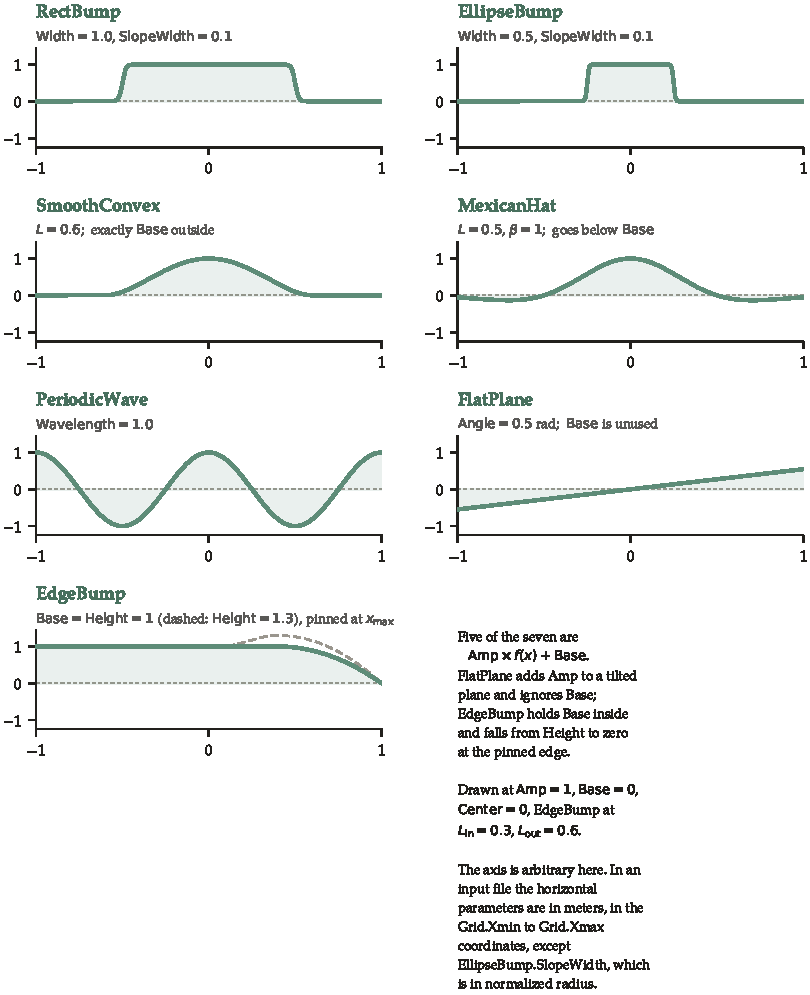
\includegraphics[width=\textwidth]{figures/shapes-1d.pdf}
  \caption{The seven shape functions, each drawn in one dimension at
    $\mathrm{Amp}=1$, $\mathrm{Base}=0$ and $\mathrm{Center}=0$ --- except
    \key{EdgeBump}, drawn as it is meant to be used, flat at
    $\mathrm{Base}=\mathrm{Height}=1$ and pinned at $x_{\max}$. Five of them
    are evaluated as $\mathrm{Amp}\times f + \mathrm{Base}$, where
    $\mathrm{Amp}$ is the block's \key{Height} --- \key{Amplitude} in
    \key{PeriodicWave} --- and $f$ is the curve drawn here; both are
    dimensionless multipliers of the container's \key{TotalHeight}. Two are
    not: \key{FlatPlane} \emph{adds} $\mathrm{Amp}$ to a tilted plane and
    ignores \key{Base} altogether, and \key{EdgeBump} holds \key{Base}
    inside and falls from \key{Height} to zero at the edge. The horizontal axis is
    arbitrary in this figure; in an input file \key{Center}, \key{Width},
    \key{Wavelength}, \key{Phase}, \key{InnerLength} and \key{OuterLength} are in meters, in
    the same coordinates as \key{Grid.Xmin} and \key{Grid.Xmax}, while
    \key{EllipseBump}'s \key{SlopeWidth} is in units of the normalized radius.
    \key{EdgeBump}'s $r_s$ is not an input key: it is derived from the domain
    edge as $x_{\max}-\key{OuterLength}$, and the panel is drawn that way. Produced by
    \file{docs/manual/\bk figures/\bk make\_shapes.py} from the definitions in
    \file{yuzen/src/\bk commonFunctions/\bk ShapeFunctions.cpp}.
    \label{fig:shapes-1d}}
\end{figure}

\subsection{How shapes combine}
\label{sec:ref-domain:createtype}

All shapes of one container are sorted by \key{Order} ascending --- ties keep
their relative order in the file --- and then applied left to right to a
running value that \textbf{starts at zero}:

\begin{description}
  \item[\val{"add"}] $\text{value} \leftarrow \max(\text{value}, \text{shape})$
    --- a \emph{union}, not a sum;
  \item[\val{"remove"}] $\text{value} \leftarrow \min(\text{value}, \text{shape})$;
  \item[\val{"stack"}] $\text{value} \leftarrow \text{value} + \text{shape}$.
\end{description}

\begin{warn}[\val{"add"} is a maximum, not an addition]
  Two overlapping bumps of height \val{0.5} combined with \val{"add"} give a
  region of height \val{0.5}, not \val{1.0}. Only \val{"stack"} adds. The
  default is \val{"add"}, so a file that lists several shapes without setting
  \key{CreateType} builds their envelope. Use \val{"add"} to place shapes side
  by side, \val{"remove"} --- a minimum --- to carve a silhouette out of what
  is already there, and \val{"stack"} to superimpose, for instance a small
  ripple on a large dome.
\end{warn}

\Cref{fig:shapes-createtype} shows the three rules applied to the same pair of
overlapping domes.

\begin{figure}[tbp]
  \centering
  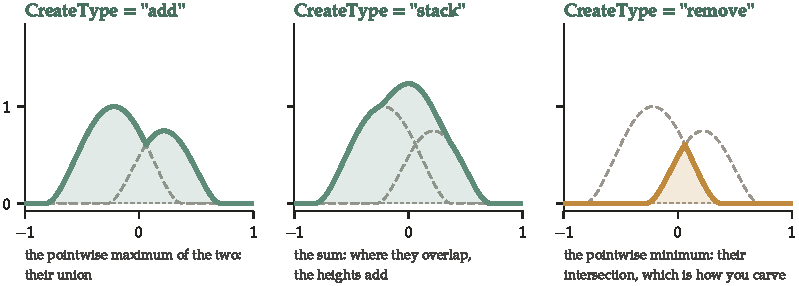
\includegraphics[width=\textwidth]{figures/shapes-createtype.pdf}
  \caption{The three merge rules of \key{CreateType}, applied to the same two
    overlapping \key{SmoothConvex} shapes (dashed). The accumulator starts at
    zero and each shape is folded into it in \key{Order}: \val{"add"} takes the
    pointwise \emph{maximum}, so it is a union and not a sum; \val{"stack"}
    takes the \emph{sum}, so overlapping heights add; \val{"remove"} takes the
    pointwise \emph{minimum}, which is how a silhouette is carved out of what
    is already there. Because the accumulator starts at zero, a shape merged
    with \val{"remove"} before anything has been added leaves nothing behind
    wherever it is positive.
    \label{fig:shapes-createtype}}
\end{figure}

Horizontal quantities --- \key{Center}, \key{Width}, \key{Wavelength},
\key{Phase}, \key{InnerLength} and \key{OuterLength}, and \key{RectBump}'s \key{SlopeWidth}
--- are in meters, in the same coordinates as \key{Grid.Xmin} and
\key{Grid.Xmax}, independently of \key{LengthScaleType}. \key{EllipseBump}'s
\key{SlopeWidth} is the exception: it softens the rim in units of the
normalized radius, so it is dimensionless. Vertical quantities --- \key{Base}, \key{Height} and
\key{Amplitude} --- are dimensionless multipliers of the container's
\key{TotalHeight}. Every \key{Center}, \key{Width}, \key{Wavelength},
\key{Phase} and \key{Angle} is an array whose length must be exactly~2, in 1-D
runs as well. A 1-D film is the line $y = 0$ of the plane the shapes are
defined in, so the $y$ components do enter: with the $y$ component of
\key{Center} and \key{Phase} at 0, as in every shipped case, each shape gives
the profile of its $x$ keys, but a bump centered further from $y = 0$ than its
$y$ extent contributes nothing, and a \key{FlatPlane} tilted in $y$ adds
$-\mathrm{Center}_y \tan \mathrm{Angle}_y$.

\subsection{\key{Initial.SurfaceShape.RectBump}}

A rectangle of height \key{Height} standing on the level \key{Base}, with
edges softened by a sigmoid so that the profile stays differentiable --- the
first panel of \cref{fig:shapes-1d}. The softening is what keeps the fourth
derivative in the height equation finite at the corners.

\begin{keytable}{Keys of \key{RectBump} (in \key{Initial.SurfaceShape} or \key{Substrate})\label{tab:shape-rectbump}}\key{Order} & int & \val{0} & Sort key; shapes are applied in ascending order. Any value. \\
\key{CreateType} & string & \val{"add"} & Merge rule: \val{"add"}, \val{"remove"} or \val{"stack"}. \\
\key{Base} & double & \val{0} & Offset added to the shape everywhere, as a fraction of \key{TotalHeight}. \\
\key{Height} & double & \val{1} & Amplitude of the bump, as a fraction of \key{TotalHeight}. \\
\key{Center} & array & \val{[0, 0]} & Center $(x,y)$ of the rectangle in meters. Length exactly~2. \\
\key{Width} & array & \val{[1, 1]} & Full width $(x,y)$ of the flat top in meters, positive. Length exactly~2. \\
\key{SlopeWidth} & array & \val{[0.05, 0.05]} & Edge-softening length $(x,y)$ in meters; internally multiplied by 0.1 to give the sigmoid width. Length exactly~2. \\
\end{keytable}

\subsection{\key{Initial.SurfaceShape.EllipseBump}}

An elliptical bump --- a flat-topped plateau with a soft rim, as the second
panel of \cref{fig:shapes-1d} shows in cross-section. The support is the
interior of $\sqrt{((x-c_x)/W_x)^2 + ((y-c_y)/W_y)^2} < 0.5$, so \key{Width}
is the \emph{full} axis length, not the semi-axis. This is the only shape any
shipped case uses.

\begin{keytable}{Keys of \key{EllipseBump} (in \key{Initial.SurfaceShape} or \key{Substrate})\label{tab:shape-ellipsebump}}\key{Order} & int & \val{0} & Sort key. \\
\key{CreateType} & string & \val{"add"} & Merge rule: \val{"add"}, \val{"remove"} or \val{"stack"}. \\
\key{Base} & double & \val{0} & Vertical offset, as a fraction of \key{TotalHeight}. \\
\key{Height} & double & \val{1} & Amplitude, as a fraction of \key{TotalHeight}. \\
\key{Center} & array & \val{[0, 0]} & Center $(x,y)$ in meters. Length exactly~2. \\
\key{Width} & array & \val{[1, 1]} & Full axes $(x,y)$ in meters, non-zero. Length exactly~2. \\
\key{SlopeWidth} & double & \val{0.05} & Edge softening of the elliptical rim, in units of the normalized radius --- a \textbf{scalar}, unlike in \key{RectBump}. \\
\end{keytable}

\begin{warn}[Work out how wide the rim actually is, in cells]
  \key{SlopeWidth} here multiplies the \emph{normalized} radius, so the width
  of the rim on the ground depends on \key{Width} as well. The profile goes
  from a tenth of \key{Height} to nine tenths of it over
  \begin{equation*}
    \Delta x \;=\; \tfrac{1}{10}\ln 81 \;\key{SlopeWidth}\,W_x
              \;\approx\; 0.44\,\key{SlopeWidth}\,W_x ,
  \end{equation*}
  and what matters is that against the cell size
  $(X_{\max}-X_{\min})/N_x$. The default \val{0.05} on a
  \SI{0.4}{\milli\metre} bump gives \SI{8.8}{\micro\metre}, half a cell on a
  60-point millimeter:
  \textbf{the default is a step on a typical mesh}, and a value written as
  though it were a length --- \val{0.1e-3}, say --- is a vertical wall.
  A wall is not merely inelegant. In \file{concz\_2d} it cuts the time step
  by a factor of 10, puts a spurious bulge of liquid in the corner
  (\SI{7.92}{\micro\metre} of film against \SI{6.05}{\micro\metre}), and
  inflates the surface excess of the concentration by a factor of 2.7. Aim for the rim to span
  several cells and check the first \file{field00000.dat} before trusting a
  long run.
\end{warn}

\subsection{\key{Initial.SurfaceShape.PeriodicWave}}

A product of cosines about the mean level \key{Base},
\[
  \text{shape} = \mathrm{Base} + \mathrm{Amplitude}\,
    \cos\!\left(\frac{2\pi (x-x_0)}{\lambda_x}\right)
    \cos\!\left(\frac{2\pi (y-y_0)}{\lambda_y}\right),
\]
useful for a corrugated substrate or for a single wavelength of a leveling
test. It is the one shape that is not localized: it fills the whole domain, and
it is as far below \key{Base} as above it (\cref{fig:shapes-1d}).

\begin{keytable}{Keys of \key{PeriodicWave} (in \key{Initial.SurfaceShape} or \key{Substrate})\label{tab:shape-periodicwave}}\key{Order} & int & \val{0} & Sort key. \\
\key{CreateType} & string & \val{"add"} & Merge rule: \val{"add"}, \val{"remove"} or \val{"stack"}. \\
\key{Base} & double & \val{0} & Mean level of the wave, as a fraction of \key{TotalHeight}. \\
\key{Amplitude} & double & \val{1} & Amplitude, as a fraction of \key{TotalHeight}. \\
\key{Wavelength} & array & \val{[1, 1]} & Wavelengths $(\lambda_x,\lambda_y)$ in meters, non-zero. Length exactly~2. \\
\key{Phase} & array & \val{[0, 0]} & Phase as a \textbf{spatial offset} $(x_0,y_0)$ in meters, not as an angle. Length exactly~2. \\
\end{keytable}

\subsection{\key{Initial.SurfaceShape.FlatPlane}}

A tilted plane,
\[
  \text{shape} = (x-c_x)\tan\alpha_x + (y-c_y)\tan\alpha_y + \mathrm{Height},
\]
that is, height \key{Height} at \key{Center} and a constant slope away from
it, as in \cref{fig:shapes-1d}. Combined with \val{"stack"} it adds a uniform
wedge to any other shape.

\begin{keytable}{Keys of \key{FlatPlane} (in \key{Initial.SurfaceShape} or \key{Substrate})\label{tab:shape-flatplane}}\key{Order} & int & \val{0} & Sort key. \\
\key{CreateType} & string & \val{"add"} & Merge rule: \val{"add"}, \val{"remove"} or \val{"stack"}. \\
\key{Height} & double & \val{1} & Height of the plane at \key{Center}, as a fraction of \key{TotalHeight}. \\
\key{Center} & array & \val{[0, 0]} & Pivot $(x,y)$ in meters about which the plane is tilted. Length exactly~2. \\
\key{Angle} & array & \val{[0, 0]} & Tilt about $x$ and $y$, in \textbf{radians}. Length exactly~2. \\
\end{keytable}

\key{FlatPlane} has \textbf{no} \key{Base} key: its constructor is always
called with a base of zero. Writing one has no effect, and no warning.

\begin{warn}[The two angles in the file are in different units]
  \key{FlatPlane.Angle} is in radians, like every other angle in the input
  file. \key{Physics.DisjoiningPressure.ContactAngle} is the single exception:
  it is in \emph{degrees}, and is range-checked against $[0:90]$. A contact
  angle written as \val{0.17} is therefore not $10^\circ$ but a sixth of a
  degree.
\end{warn}

\subsection{\key{Initial.SurfaceShape.MexicanHat}}

The Ricker wavelet: a central peak surrounded by a circular trough. Unlike the
other localized shapes it dips \emph{below} \key{Base} around its peak, and it
never quite returns to it, which \cref{fig:shapes-1d} makes plain at a glance:
\[
  \text{shape} = \mathrm{Base} + \mathrm{Height}\,(1-r^2)\,e^{-\beta r^2},
  \qquad
  r^2 = \left(\frac{x-c_x}{L_x}\right)^{2} + \left(\frac{y-c_y}{L_y}\right)^{2}.
\]

\begin{keytable}{Keys of \key{MexicanHat} (in \key{Initial.SurfaceShape} or \key{Substrate})\label{tab:shape-mexicanhat}}\key{Order} & int & \val{0} & Sort key. \\
\key{CreateType} & string & \val{"add"} & Merge rule: \val{"add"}, \val{"remove"} or \val{"stack"}. \\
\key{Base} & double & \val{0} & Vertical offset, as a fraction of \key{TotalHeight}. \\
\key{Height} & double & \val{1} & Amplitude, as a fraction of \key{TotalHeight}. \\
\key{Center} & array & \val{[0, 0]} & Center $(x,y)$ in meters. Length exactly~2. \\
\key{Width} & array & \val{[1, 1]} & Radial scales $(L_x,L_y)$ in meters. Length exactly~2; a zero component makes the shape vanish everywhere. \\
\key{Beta} & double & \val{1} & Decay $\beta$ of the Gaussian envelope, non-dimensional; non-negative in practice. \\
\end{keytable}

\subsection{\key{Initial.SurfaceShape.SmoothConvex}}

A compact dome, $\mathrm{Height}\,(1-r^2)^2$ inside $r\le 1$ and exactly
\key{Base} outside it, with $r$ defined as for \key{MexicanHat}. Unlike an
ellipsoid it meets the surrounding level with zero slope, so it introduces no
curvature spike at its rim; compare its shoulders with those of
\key{MexicanHat} in \cref{fig:shapes-1d}.

\begin{keytable}{Keys of \key{SmoothConvex} (in \key{Initial.SurfaceShape} or \key{Substrate})\label{tab:shape-smoothconvex}}\key{Order} & int & \val{0} & Sort key. \\
\key{CreateType} & string & \val{"add"} & Merge rule: \val{"add"}, \val{"remove"} or \val{"stack"}. \\
\key{Base} & double & \val{0} & Level outside the support, returned verbatim for $r>1$, as a fraction of \key{TotalHeight}. \\
\key{Height} & double & \val{1} & Peak amplitude, as a fraction of \key{TotalHeight}. \\
\key{Center} & array & \val{[0, 0]} & Center $(x,y)$ in meters. Length exactly~2. \\
\key{Width} & array & \val{[1, 1]} & Radial half-extents $(L_x,L_y)$ in meters, non-zero. Length exactly~2. \\
\end{keytable}

\subsection{\key{Initial.SurfaceShape.EdgeBump}}

The film against a pinned edge: flat at \key{Base} inside the domain, it falls
to zero at the edge over the last \key{OuterLength} --- the last panel of
\cref{fig:shapes-1d}. It exists to start a run from a film that is already
pinned at a wall, with a meniscus, instead of from a discontinuity. With $p$
the distance from the switch-over point $r_s$, which lies \key{OuterLength}
inside the edge, positive toward the edge, the profile is
%
\begin{equation}
  f(p) = \bigl(1-\sigma(p)\bigr)\Bigl[(H-B)\,\bigl(1-p^2/L_i^2\bigr)\,e^{-p^2/(\alpha L_i^2)} + B\Bigr]
       + \sigma(p)\,H\,\bigl(1 - p^2/L_o^2\bigr),
\end{equation}
%
with $B$ = \key{Base}, $H$ = \key{Height}, $L_i$ = \key{InnerLength}, $L_o$ =
\key{OuterLength}, $\alpha$ = \key{Alpha} and $\sigma$ a logistic step of width
$0.1\,L_i$ at $r_s$. \textbf{The usual setting is $\mathrm{Height} =
\mathrm{Base}$} (for a film of uniform thickness, both 1): the film is flat up
to $r_s$ and falls as a parabola to zero at the edge. A \key{Height} above
\key{Base} raises a rim at $r_s$ (the dashed curve of the figure), one below it
a dip.

\textbf{\key{EdgeBump} exists only inside \key{Initial.SurfaceShape}}; the
\key{Substrate} block does not accept it.

\begin{keytable}{Keys of \key{Initial.SurfaceShape.EdgeBump}\label{tab:shape-edgebump}}\key{Order} & int & \val{0} & Sort key. \\
\key{CreateType} & string & \val{"add"} & Merge rule: \val{"add"}, \val{"remove"} or \val{"stack"}. \\
\key{Base} & double & \val{0} & Level of the film inside the domain, away from the edge, as a fraction of \key{TotalHeight}. \\
\key{Height} & double & \val{1} & Level at the switch-over point \key{OuterLength} inside the edge, from which the film falls to zero at the edge; equal to \key{Base} for a film flat up to the meniscus. \\
\key{Location} & string & \val{"Xmax"} & Which domain edge the bump is attached to: \val{"Xmin"}, \val{"Xmax"}, \val{"Ymin"} or \val{"Ymax"}. The matching \key{Boundary} block must be of type \val{"Pinning"}. \\
\key{Alpha} & double & \val{1} & Width parameter $\alpha>0$ of the inner Gaussian $\exp(-(1/\alpha)(p/\mathrm{InnerLength})^2)$, non-dimensional. \\
\key{InnerLength} & double & \val{1} & Inner length scale in meters, positive; also sets the blending width, $0.1\,\mathrm{InnerLength}$. \\
\key{OuterLength} & double & \val{1} & Width of the meniscus in meters: the distance from the edge to the switch-over point, over which the film falls to zero. \\
\end{keytable}

A pinned edge needs a film that reaches zero there, and \key{EdgeBump} is the
shape that provides one: its profile falls to zero at the wall whatever
\key{Base} and \key{Height} are, which with a small \key{PrecursorRatio} leaves only the precursor. The
solver checks the result before the first step (\cref{sec:ref-bcout:boundary}).

\begin{note}[\key{Location} and the boundary condition must agree]
  \code{CheckParameters} rejects the input unless the
  \key{Boundary.<Location>BC.Type} matching every \key{EdgeBump} is
  \val{"Pinning"}, with the message \code{Input mismatch}. It is one of the
  cross-key constraints checked before the model is built; that the film then
  reaches zero at the pinned edge is checked just before the first step
  (\cref{sec:ref-bcout:boundary}).
\end{note}

\section{\key{Substrate}}
\label{sec:ref-domain:substrate}

\key{Substrate} is optional and may appear at most once. It describes the
solid surface $s(x,y)$ that the film sits on. The substrate never moves and
never changes. It enters the capillary-pressure and vertical-gravity terms
through the free-surface height $h+s$, so \textbf{if neither of those two terms
is enabled the substrate shape does nothing at all}
(\cref{sec:terms:laplace,sec:terms:vgravity}).

If the block is absent the substrate is flat: no shape is registered and the
profile is never evaluated.

\begin{keytable}{Keys of \key{Substrate}\label{tab:substrate-keys}}\key{TotalHeight} & double & \val{1} & Height scale of the topography in meters; the profile is \key{TotalHeight} times the combined shape. Independent of \key{Initial.SurfaceShape.TotalHeight}. \\
\end{keytable}

\key{Substrate} accepts the same repeatable shape blocks as
\key{Initial.SurfaceShape} \textbf{except \key{EdgeBump}} --- that is,
\key{RectBump}, \key{EllipseBump}, \key{PeriodicWave}, \key{FlatPlane},
\key{MexicanHat} and \key{SmoothConvex} --- with identical key names, types,
defaults, ranges and units. The two parsers are the same code writing into a
different destination, so \cref{tab:shape-rectbump,tab:shape-ellipsebump,tab:shape-periodicwave,tab:shape-flatplane,tab:shape-mexicanhat,tab:shape-smoothconvex}
apply unchanged. The only other difference is that \key{Base}, \key{Height}
and \key{Amplitude} are fractions of \key{Substrate.TotalHeight} here.

\begin{note}[The substrate ordering path is untested]
  No case in \file{cases/} sets \key{Order} inside a \key{Substrate} shape
  block, and no case uses any substrate shape other than \key{EllipseBump}.
  If you build a substrate from several shapes, check the result in the first
  field output before trusting it.
\end{note}

\section{\key{Fluid}}
\label{sec:ref-domain:fluid}

\key{Fluid} is required and appears exactly once. It has one key of its own,
and five sub-blocks that are \textbf{all required} --- a missing one aborts the
run --- even though every key inside them has a default.

\begin{keytable}{Keys of \key{Fluid}\label{tab:fluid-keys}}\key{Name} & string & \val{"CR-EX"} & Label for the liquid. Recorded and printed in the log only; it selects no property set. \\
\end{keytable}

\subsection{Concentration dependence}
\label{sec:ref-domain:fluidconc}

Three of the five sub-blocks give a property at a reference concentration and
the way it varies around it. These three laws are what the \key{BaseValue},
\key{BaseConc}, \key{Coef} and \key{Exponent} keys mean:

\begin{align}
  \sigma(c) &= \mathrm{BaseValue} + \mathrm{Coef}\,(c - \mathrm{BaseConc}),
    \label{eq:fluid-sigma}\\
  \mu(c)    &= \mathrm{BaseValue}\,
    \exp\bigl(\mathrm{Exponent}\,(c - \mathrm{BaseConc})\bigr),
    \label{eq:fluid-mu}\\
  D(c)      &= \mathrm{BaseValue}\,
    \exp\bigl(\mathrm{Exponent}\,(c - \mathrm{BaseConc})\bigr).
    \label{eq:fluid-diff}
\end{align}

Surface tension is linear in concentration; viscosity and diffusivity are
exponential. \Cref{eq:fluid-mu} is the strongest non-linearity in the solver:
with \key{Exponent} near 10, a concentration change of 0.1 multiplies the
viscosity by $e$, and it is this that stops the flow as the film dries.
\Cref{eq:fluid-sigma} feeds two different places --- the slope \key{Coef} is
the Marangoni number $\Ma$, and $\sigma(c)$ also enters the mobility of the
capillary-pressure term, so drying changes how fast the film levels
(\cref{ch:concentration}).

\subsection{\key{Fluid.Density}}

\begin{keytable}{Keys of \key{Fluid.Density}\label{tab:fluid-density-keys}}\key{Value} & double & \val{1070} & Liquid density $\rho$ in \si{\kilogram\per\metre\cubed}, positive. Assumed independent of concentration. Enters the capillary length $L_0$, and the groups $\Bo$, $\Pvec$ and $\Spn$. \\
\end{keytable}

\subsection{\key{Fluid.SurfaceTension}}

\begin{keytable}{Keys of \key{Fluid.SurfaceTension}, see \cref{eq:fluid-sigma}\label{tab:fluid-surften-keys}}\key{BaseValue} & double & \val{0.028} & Surface tension $\sigma_0$ at \key{BaseConc}, in \si{\newton\per\metre}, positive. Sets the capillary length and the time scale. \\
\key{BaseConc} & double & \val{0.5} & Reference concentration of the linear law, mass fraction in $[0:1]$. \\
\key{Coef} & double & \val{0.014} & $\mathrm{d}\sigma/\mathrm{d}c$ in \si{\newton\per\metre} per unit concentration; the sign matters. Its ratio to \key{BaseValue} is the Marangoni number $\Ma$. Forced to zero when \key{Physics.SolutoCapillarity.Enable} is false. \\
\end{keytable}

\subsection{\key{Fluid.Viscosity}}

\begin{keytable}{Keys of \key{Fluid.Viscosity}, see \cref{eq:fluid-mu}\label{tab:fluid-visc-keys}}\key{BaseValue} & double & \val{0.115} & Viscosity $\mu_0$ at \key{BaseConc}, in \si{\pascal\second}, positive. Sets the time scale $T_0 = \mu_0 L_0^4/(\sigma_0 h_0^3)$. \\
\key{BaseConc} & double & \val{0.5} & Reference concentration, mass fraction in $[0:1]$. \\
\key{Exponent} & double & \val{8} & Exponential rate, non-dimensional, any value. A realistic figure is about 10, i.e.\ $\Delta c = 0.1$ multiplies $\mu$ by $e$. \\
\end{keytable}

\subsection{\key{Fluid.Diffusivity}}

\begin{keytable}{Keys of \key{Fluid.Diffusivity}, see \cref{eq:fluid-diff}\label{tab:fluid-diff-keys}}\key{BaseValue} & double & \val{9.78e-11} & Solute diffusivity $D_0$ at \key{BaseConc}, in \si{\metre\squared\per\second}, positive. Enters $\Pen = E_0 h_0/D_0$ and $\Df = D_0 T_0/L_0^2$. \\
\key{BaseConc} & double & \val{0.5} & Reference concentration, mass fraction in $[0:1]$. \\
\key{Exponent} & double & \val{6.94} & Exponential rate, non-dimensional, any value; usually negative in practice. \\
\end{keytable}

\subsection{\key{Fluid.MolarMass}}

Only the ratio $\Mr = \mathrm{Resin}/\mathrm{Solvent}$ is used, in Raoult's law
for the evaporation rate (\cref{sec:terms:evaporation}), so any consistent
pair of units will do.

\begin{keytable}{Keys of \key{Fluid.MolarMass}\label{tab:fluid-molar-keys}}\key{Solvent} & double & \val{106} & Molar mass of the solvent, positive; \si{\gram\per\mole} in practice, but any unit consistent with \key{Resin}. \\
\key{Resin} & double & \val{2200} & Molar mass of the solute, positive, in the same unit as \key{Solvent}. \\
\end{keytable}

% ch-ref-physics.tex -- reference: the Physics block and its nine sub-blocks
\chapter{Physics}
\label{ch:ref-physics}

\key{Physics} is required and must appear exactly once, but it carries no keys
of its own. It is a container for nine sub-blocks, one per physical effect,
each of which is optional and may appear at most once. Almost all of them are
switched with a single \key{Enable} key, and the term they control contributes
a coefficient to the flux in the height equation; when a term is disabled its
dimensionless group is set to zero and the term is not assembled.

This chapter lists the keys. What each term \emph{is} --- the flux it adds and
the assumptions behind it --- is in the theory part, which each section points
to.

\begin{note}[An absent \key{Physics} sub-block is a term switched off]
  A sub-block left out of the file reads as an empty one with its switch
  off: the term is not computed, and every other key takes the default listed
  in this chapter. For the four sub-blocks whose \key{Enable} defaults to
  \val{true} --- \key{LaplacePressure}, \key{SolutoCapillarity},
  \key{Evaporation} and \key{Source} --- leaving the block out is therefore
  not the same as writing it empty: an empty \code{[Physics.Evaporation]}
  switches evaporation on, a missing one leaves it off. A missing
  \key{ConcField} means \key{Model}~$=$~\val{"None"}. Every shipped case
  writes each sub-block it relies on.
\end{note}

\section{\key{Physics.ConcField}}
\label{sec:ref-physics:concfield}

This block decides how, or whether, the solute is transported, and its
\key{Model} key together with \key{Grid.Dimension} selects the whole solver
model. \val{"WM"} with \val{"xh"} gives the 1-D well-mixed model, \val{"WM"} with
\val{"xyh"} the 2-D one, \val{"CZ"} with \val{"xh"} the model that resolves
concentration through the thickness over a 1-D film, and \val{"CZ"} with
\val{"xyh"} the same over a 2-D film (the pseudo-3D case).
See \cref{ch:concentration}.

\begin{keytable}{Keys of \key{Physics.ConcField}\label{tab:physics-concfield-keys}}\key{Model} & string & \reqd & \val{"WM"} = well-mixed, depth-averaged concentration solved alongside the film; \val{"CZ"} = concentration resolved through the thickness, over a 1-D or a 2-D film (needs $\mathrm{Nz}\ge 2$); \val{"None"} = no concentration equation; \val{"CZ\_flow"} = accepted but not implemented. Required whenever the block is present; without the block the model is \val{"None"}. \\
\key{EnableConvection} & bool & \val{true} & Include the convective term in the concentration equation. Well-mixed models only. \\
\key{EnableDiffusion} & bool & \val{true} & Include the diffusive term in the concentration equation. Well-mixed models only. \\
\end{keytable}

\begin{warn}[\val{"CZ\_flow"} passes the range check and then does nothing]
  \val{"CZ\_flow"} is in the candidate list, so it is accepted without
  complaint, but no model implements it. The run falls back to the well-mixed
  model chosen by \key{Grid.Dimension} \emph{with the concentration equation
  switched off} --- the same thing \val{"None"} does, and the same thing an
  unknown string does if it somehow passes the check. The result is a
  plausible-looking run at constant concentration. Do not use it.
\end{warn}

When the concentration equation is not built --- \val{"None"}, \val{"CZ\_flow"}
or an unknown string --- \key{EnableConvection}, \key{EnableDiffusion},
\key{Fluid.Diffusivity} and the whole of \key{Numerics.ConcEquation} have no
effect.

\section{\key{Physics.LaplacePressure}}
\label{sec:ref-physics:laplace}

The surface-tension term: the tendency of the free surface to flatten itself.
It is what levels a film, what makes a drop a spherical cap, and what pulls
liquid into the dips of a rough substrate. It contains a fourth spatial
derivative, and it is the reason the height equation is fourth order, so
essentially every run keeps it on. The curvature is measured on the free
surface $h+s$, not on the film thickness, which is how the substrate shape
enters. See \cref{sec:terms:laplace}.

\begin{keytable}{Keys of \key{Physics.LaplacePressure}\label{tab:physics-laplace-keys}}\key{Enable} & bool & \val{true} & Switch on the capillary (Laplace) pressure term of the height equation. \\
\end{keytable}

\section{\key{Physics.SolutoCapillarity}}
\label{sec:ref-physics:soluto}

Solutal Marangoni flow: because surface tension depends on concentration, a
concentration gradient is a surface stress that drags liquid along the free
surface. It scales with $h^2$ rather than $h^3$, since it is a shear applied at
the surface rather than a body force, and it is a common origin of drying
streaks and coating mottle. See \cref{sec:terms:marangoni}.

\begin{keytable}{Keys of \key{Physics.SolutoCapillarity}\label{tab:physics-soluto-keys}}\key{Enable} & bool & \val{true} & Switch on solutal Marangoni flow. When false, $\Ma$ is forced to 0 and \key{Fluid.SurfaceTension.Coef} is silently ignored. \\
\end{keytable}

\begin{warn}[Disabling it also makes surface tension concentration-independent]
  $\Ma$ is not only the coefficient of the Marangoni stress; it is also what
  makes $\sigma$ depend on $c$ in the mobility of the capillary-pressure term.
  Setting \key{Enable = false} therefore removes the concentration dependence
  of surface tension \emph{entirely}, so that a drying film levels at the rate
  set by $\sigma_0$ alone. If you want the dependence without the Marangoni
  stress, this switch will not give it to you.
\end{warn}

\section{\key{Physics.DisjoiningPressure}}
\label{sec:ref-physics:disjoining}

The disjoining pressure
$\Pihat = (\Hstar/H)^n - (\Hstar/H)^m$ represents the interaction between
substrate and free surface once the film becomes very thin. It is what gives
the model partial wetting: a finite equilibrium contact angle, a moving contact
line, and a precursor film of thickness $\Hstar$ left outside the drop. Its
coefficient is fixed so that the angle you ask for is the one reproduced in the
lubrication limit, so changing the exponents or the precursor ratio does not
change the target angle --- it changes the thickness of the precursor and the
width of the transition region. Because $\Pihat \sim H^{-n}$, this is by a wide
margin the stiffest term in the model. See \cref{sec:terms:disjoining}.

\begin{keytable}{Keys of \key{Physics.DisjoiningPressure}\label{tab:physics-disjoining-keys}}\key{Enable} & bool & \val{false} & Switch on the disjoining pressure, i.e.\ partial wetting with a finite contact angle. Requires \key{Initial.SurfaceShape.PrecursorRatio} $>0$. \\
\key{ContactAngle} & double & \val{0} & Equilibrium contact angle $\thetae$ in \textbf{degrees}, range $[0:90]$, checked only when \key{Enable} is true. \val{0} gives zero disjoining pressure. \\
\key{ExponentN} & double & \val{3} & Exponent $n$ of the repulsive branch, non-dimensional. Must satisfy $n>m>1$, checked only when \key{Enable} is true. \\
\key{ExponentM} & double & \val{2} & Exponent $m$ of the attractive branch, non-dimensional, subject to the same constraint. \\
\end{keytable}

\begin{note}[The exponents default to $(n,m)=(3,2)$]
  Whether the block is absent or is written with \key{Enable = true} and no
  exponents, the pair is $(3,2)$.
\end{note}

\begin{warn}[A zero precursor ratio with disjoining pressure enabled aborts]
  $\Hstar$ is the thickness at which $\Pihat$ vanishes, so it cannot be zero.
  \key{Initial.SurfaceShape.PrecursorRatio = 0} together with
  \key{Enable = true} is fatal in \code{NonDimensionalNumbers::Build}, before
  any step is taken. The message in \file{FatalErrors.txt} reads
  \code{Physics.DisjoiningPressure requires
  Initial.SurfaceShape.PrecursorRatio > 0.}
  (\cref{sec:output:warnings}). Sizing the precursor is a modeling decision,
  not a formality: see \cref{sec:terms:disjoining}.
\end{warn}

\begin{note}[The \val{"CZ"} model ignores this block entirely]
  With \key{Physics.ConcField.Model = "CZ"} the height equation is built from
  capillary pressure, solutocapillarity, centrifugal force, vertical gravity
  and horizontal gravity only. \key{Physics.DisjoiningPressure} and the whole
  of \key{Physics.Source} have no effect, silently. Contact-line problems
  belong to the well-mixed models.
\end{note}

\section{\key{Physics.VerticalGravity}}
\label{sec:ref-physics:vgravity}

Gravity normal to the substrate: hydrostatic pressure drives liquid from high
parts of the free surface to low ones, so on a horizontal substrate it flattens
bumps and works alongside capillary pressure. Like capillary pressure it is
driven by $h+s$, so it too feels the substrate shape. If you are tilting the
substrate by an angle $\alpha$, the value to give here is $g\cos\alpha$. See
\cref{sec:terms:vgravity}.

\begin{keytable}{Keys of \key{Physics.VerticalGravity}\label{tab:physics-vgravity-keys}}\key{Enable} & bool & \val{false} & Switch on the hydrostatic, film-leveling gravity term. When false, $\Bo$ is forced to 0. \\
\key{Acceleration} & double & \val{9.80665} & Acceleration normal to the substrate in \si{\metre\per\second\squared}, non-negative; gives the Bond number $\Bo = \rho g L_0^2/\sigma_0$. Read even when \key{Enable} is false, and then discarded. \\
\end{keytable}

With the capillary length scale and \key{Acceleration = 9.80665} the Bond number is
exactly 1; \key{Acceleration} is the key to change when you want to move $\Bo$.

\section{\key{Physics.HorizontalGravity}}
\label{sec:ref-physics:hgravity}

An in-plane body force, that is, an inclined substrate. Unlike vertical
gravity the driving field is a constant vector independent of position, so
thicker parts of the film run faster and a front forms. For a substrate tilted
by $\alpha$, give the in-plane component $g\sin\alpha$ --- \num{4.903} at
$30^\circ$ --- and let its sign set the downhill direction. See
\cref{sec:terms:hgravity}.

\begin{keytable}{Keys of \key{Physics.HorizontalGravity}\label{tab:physics-hgravity-keys}}\key{Enable} & bool & \val{false} & Switch on the in-plane body force. When false, $\Pgx$ and $\Pgy$ are forced to 0. \\
\key{Acceleration} & array & \val{[0, 0]} & In-plane acceleration $(g_x,g_y)$ in \si{\metre\per\second\squared}. Length must be exactly~2, in 1-D runs as well. \\
\end{keytable}

\section{\key{Physics.Centrifugal}}
\label{sec:ref-physics:centrifugal}

The centrifugal term of spin coating: a rotating substrate throws the film
outwards, with a driving field proportional to the distance $r$ from the axis,
so the effect is strongest at the rim. In a 1-D (\val{"xh"}) run the liquid
thrown into the unsolved $y$ direction is accounted for as outflow, and
counted in \code{OutflowedVol} of \file{History.dat}. A rotating film is not
periodic, and a \val{"Periodic"} edge is refused with this term (except under
\key{Numerics.ManufacturedSolution}). See \cref{sec:terms:centrifugal}.

\begin{keytable}{Keys of \key{Physics.Centrifugal}\label{tab:physics-centrifugal-keys}}\key{Enable} & bool & \val{false} & Switch on the centrifugal (spin-coating) term. When false, $\Spn$ is forced to 0. \\
\key{RotationRate} & double & \val{0} & Angular velocity $\omega$ of the substrate in \si{\radian\per\second}, any value; $\Spn = \rho\omega^2 L_0^4/(\sigma_0 h_0)$. \\
\key{RotationAxis} & array & \val{[0, 0]} & In-plane position $(x,y)$ of the rotation axis, in meters. Length must be exactly~2. \\
\end{keytable}

\section{\key{Physics.Slip}}
\label{sec:ref-physics:slip}

A Navier slip length $\lambda$ at the substrate: the fluid slides over it with
the velocity $\lambda\,\partial u/\partial z$. Every term driven by a pressure
or a body force then has the mobility $h^{3}/3 + \lambda h^{2}$ in place of
$h^{3}/3$, and the Marangoni term $h^{2}/2 + \lambda h$ in place of $h^{2}/2$
(\cref{sec:terms:slip}). The dimensionless slip length is
$\Lambda = \lambda/h_0$, printed as \code{Lambda} under
\code{Nondimensional numbers} of the log when slip is on. Slip changes the
dynamics only: an equilibrium is the same with it. A missing block is no
slip; so is \key{Enable = true} with \key{Length = 0} (with a warning). The
\val{"CZ"} model refuses the block (\cref{ch:notverified}). With slip the
positivity of the film is guaranteed at one order less
(\cref{sec:disc:positivity-slip}).

\begin{keytable}{Keys of \key{Physics.Slip}\label{tab:physics-slip-keys}}\key{Enable} & bool & \val{false} & Switch on Navier slip at the substrate. When false, $\Lambda = 0$ and every term runs its no-slip expressions, bit for bit. \\
\key{Length} & double & \val{0.0} & Slip length $\lambda$ in meters, non-negative; $\Lambda = \lambda/h_0$. \\
\end{keytable}

\section{\key{Physics.Evaporation}}
\label{sec:ref-physics:evaporation}

Evaporation removes solvent, so the film thins and what is left grows more
concentrated. The rate is a product of a reference velocity, a function of
concentration, a function of position and a thin-film correction; the
concentration equation receives the same rate divided by the local thickness,
which is why thin regions concentrate fastest. See
\cref{sec:terms:evaporation}.

\begin{keytable}{Keys of \key{Physics.Evaporation}\label{tab:physics-evap-keys}}\key{Enable} & bool & \val{true} & Switch on solvent evaporation. When false the evaporation model is not built at all and the rate is 0 everywhere. \\
\key{Coef} & double & \val{1} & Reference evaporation velocity $E_0$ in \si{\metre\per\second}, non-negative; gives $\Ev = E_0 T_0/h_0$ and $\Pen = E_0 h_0/D_0$. \\
\key{SpatialFunc} & string & \val{"uniform"} & Spatial distribution of the flux: \val{"uniform"}, or \val{"negPow"}, the radial power $k(1-r/R')^{-n}$ of \cref{eq:evap-negpow}, which for $n>0$ diverges as a negative power toward the rim of the pool (capped at 10), blended over 5 cells into a quarter cosine that takes over the curve's value and slope, peaks at \key{NegPowRmax} and is constant beyond it. \\
\key{ConcFunc} & string & \val{"Raoult"} & Concentration dependence: \val{"Raoult"} for Raoult's law using the molar-mass ratio, or \val{"PowerN"} for $\max(1-c-\mathrm{ConcR},0)^{\mathrm{PowerN}}$. \\
\key{NegPowExponent} & double & \val{0.25} & Exponent $n$ of the \val{"negPow"} distribution $k(1-r/R')^{-n}$, non-dimensional, less than 1: positive gives a rate diverging at the rim, 0 a uniform one, negative one falling to zero there; the prefactor $k=\frac{1}{2}(1-n)(2-n)$ keeps the mean over the pool at 1. Used only when \key{SpatialFunc} is \val{"negPow"}. \\
\key{NegPowRmax} & double & \val{1} & Radius $R$ of the pool of the \val{"negPow"} distribution in meters, positive, measured from the origin of the grid coordinates. Used only with \val{"negPow"}. \\
\key{PowerN} & double & \val{0.5} & Exponent of the \val{"PowerN"} law, non-dimensional, any value; with 0 the rate does not fall with $c$, and the solvent limit stops it at $c = 1$ (\cref{sec:terms:evaporation}). Used only with \val{"PowerN"}. \\
\key{ConcR} & double & \val{0.0} & Residual concentration offset in the \val{"PowerN"} law, mass fraction in $[0:1)$: evaporation stops at $c = 1-\mathrm{ConcR}$. Used only with \val{"PowerN"}. \\
\key{EndConcType} & string & \val{"mean"} & Which concentration statistic is compared against \key{EndConcValue}: \val{"mean"}, \val{"max"} or \val{"min"}; any other string is refused. \\
\key{EndConcValue} & double & \val{0.95} & Dry-out threshold, mass fraction in $(0:1]$. The run stops with \code{Dry out} as soon as the chosen statistic exceeds it. \\
\end{keytable}

\begin{warn}[The dry-out test runs even with evaporation disabled]
  \key{EndConcValue} is applied whether or not \key{Enable} is true, and a
  file that leaves \key{Physics.Evaporation} out gets the default
  \val{0.95}. A film whose concentration reaches the threshold by any other
  route therefore stops with \code{Dry out} even with evaporation off.
\end{warn}

\key{PowerN}, \key{ConcR},
\key{EndConcType} and \key{EndConcValue} are not exercised by any case in
\file{cases/}.

\section{\key{Physics.Source}}
\label{sec:ref-physics:source}

Liquid supplied to the film through a nozzle, optionally carried on a rotating
arm --- the model of a dispensing head. Each cell receives supply in
proportion to the fraction of it that the nozzle footprint covers, and that
fraction is measured by subdividing the cell. See \cref{sec:terms:source}.

\begin{keytable}{Keys of \key{Physics.Source}\label{tab:physics-source-keys}}\key{Enable} & bool & \val{true} & Switch on the source term. Note the default is \textbf{true}: writing the block without \key{Enable} turns the nozzle on; leaving the block out leaves it off. \\
\key{Radius} & double & \val{1} & Radius of the nozzle footprint in meters, positive. \\
\key{InletRate} & double & \val{0} & Steady-state supply velocity in \si{\metre\per\second} (volume flux per unit area), non-negative; non-dimensionalized by $h_0/T_0$. \\
\key{ConcType} & string & \val{"local"} & The concentration the supplied liquid arrives at: \val{"local"}, that of the film where it lands (it thickens the film without changing $c$); \val{"supplied"}, \key{Conc}, mixed through the thickness of the column it lands on (\cref{sec:terms:source}). Any other string is refused. \\
\key{Conc} & double & \val{0} & Concentration of the supplied liquid, mass fraction in $[0:1]$; outside it is refused with \key{ConcType = "supplied"}. Used only with \val{"supplied"}. \\
\key{TimeConstant} & double & \val{0} & Exponential rise time $\tau$ of the flow rate in seconds, non-negative: $\mathrm{rate} = \mathrm{InletRate}\,(1-e^{-t/\tau})$. \val{0} means full rate from the first step. \\
\key{ArmLength} & double & \val{1} & Length of the rotating arm carrying the nozzle, in meters, non-negative. \val{0} pins the nozzle at \key{ArmCenter}. \\
\key{ArmCenter} & array & \val{[0, 0]} & Position $(x,y)$ of the arm pivot, in meters. Length must be exactly~2. \\
\key{RotationRate} & double & \val{0} & Angular velocity of the arm in \si{\radian\per\second}, any value. Distinct from \key{Physics.Centrifugal.RotationRate}. \\
\key{StartAngle} & double & \val{0} & Arm angle at $t=0$, in radians, any value. \\
\key{RampTime} & double & \val{0} & Ramp-up and ramp-down time of the arm's rotation rate in seconds, non-negative. \\
\key{PlateauTime} & double & \val{1e10} & How long the rotation rate stays at its plateau before ramping down, in seconds, non-negative. \\
\key{SubRegions} & int & \val{1} & Number of sub-divisions per cell used when measuring the covered fraction, at least 1. Larger values smooth the source as the nozzle moves. \\
\end{keytable}

\begin{note}[\key{ConcType} decides whether \key{Conc} is used]
  By default (\key{ConcType = "local"}) the supplied liquid takes the
  concentration already present where it lands, and \key{Conc} is not used:
  setting it alone does not dispense liquid of a different composition. With
  \key{ConcType = "supplied"} the liquid arrives at \key{Conc}, and the
  concentration under the nozzle follows from mixing it into the film
  (\cref{eq:source-mixing}). \code{SuppliedResin} in \file{History.dat}
  counts the solute either way brings. Without a concentration equation
  (\key{Physics.ConcField.Model = "None"}) the key has no effect.
\end{note}

% ch-ref-boundary-output.tex -- reference: the Boundary and Output blocks
\chapter{Boundary conditions and output}
\label{ch:ref-bcout}

Two blocks are documented here. \key{Boundary} decides what happens at the
edges of the domain, which is one of the choices that most strongly changes the
answer; \key{Output} decides what is written to disk and how often, which
decides whether you can tell what happened. Both are required and both appear
exactly once.

\section{\key{Boundary}}
\label{sec:ref-bcout:boundary}

\key{Boundary} carries no keys of its own. It contains one sub-block per
domain edge, each with exactly one key, \key{Type}. \key{XminBC} and
\key{XmaxBC} are required; \key{YminBC} and \key{YmaxBC} are optional and are
only meaningful when \key{Grid.Dimension} is \val{"xyh"}.

\begin{keytable}{The four sub-blocks of \key{Boundary}, each with the single key \key{Type}\label{tab:boundary-keys}}\key{XminBC.Type} & string & \val{"Symmetry"} & Condition on the $x=\mathrm{Xmin}$ edge: \val{"Symmetry"}, \val{"Periodic"}, \val{"Pinning"}, \val{"FreshInlet"} or \val{"Outlet"}. The block is required. \\
\key{XmaxBC.Type} & string & \val{"Symmetry"} & Condition on the $x=\mathrm{Xmax}$ edge, same set of values. The block is required. \\
\key{YminBC.Type} & string & \val{"Symmetry"} & Condition on the $y=\mathrm{Ymin}$ edge, same set of values. The block is optional and is ignored in 1-D. \\
\key{YmaxBC.Type} & string & \val{"Symmetry"} & Condition on the $y=\mathrm{Ymax}$ edge, same set of values. The block is optional and is ignored in 1-D. \\
\end{keytable}

\begin{note}[Two conditions per edge, because the equation is fourth order]
  The height equation contains a fourth spatial derivative, so each boundary
  needs \emph{two} conditions, not one. That is why you choose a named type
  rather than writing a value: each name stands for a pair of conditions, and
  the ghost layer is two cells deep so that the pair can be imposed. The
  concentration equation is second order and takes one condition from the same
  name.
\end{note}

\subsection{What each type means}

\paragraph{\val{"Symmetry"}} A plane of symmetry: no flux crosses the
boundary, and both the shape and the concentration are mirrored through it,
$\partial h/\partial n = 0$ and $\partial^3 h/\partial n^3 = 0$: the two ghost
layers are the exact mirror image of the two layers inside, in 1-D as in 2-D
(\cref{sec:time:apply}). Use it to put
the center of a drop or a film on the boundary and halve the cost, or as a
closed wall. It is the default. It is the wrong choice whenever liquid should
be able to leave: a drop spreading toward a \val{"Symmetry"} edge behaves as
if a wall stood there, and gives a different answer from \val{"Outlet"}.

\paragraph{\val{"Periodic"}} The edge is joined to the opposite one; the ghost
layers are copied across. Use it for a film on a periodically structured
substrate, or to compute one wavelength of a pattern that continues for ever.
It is the wrong choice when the physics has a net drift across the domain ---
with in-plane gravity or a source, periodicity recycles what flows out of one
side back into the other. With the centrifugal term it is refused: the arm of
the force, the distance from the rotation axis, jumps by the length of the
domain across the seam, so a rotating film is not periodic
(\cref{sec:terms:centrifugal}; a run with a manufactured solution is
exempt).

\paragraph{\val{"Pinning"}} The contact line is held at the edge: the film
thickness at the boundary is pinned to zero and the in-plane velocity there is
zero, while the concentration takes a zero-gradient condition. Because the thickness is held at zero, \textbf{the initial film must reach
zero at a pinned edge too}, and the solver checks it before the first step: it
extrapolates the film from the first two cells to the wall and reports the
value in the run log,
\begin{plain}
Pinning Xmax: the initial film reaches 0.204 um at the wall (2.0 % of its 9.995 um maximum) -- ok.
\end{plain}
and stops the run, with that line and what to do, if more than a tenth of the
thickest film is left at the wall. A film of full thickness against a pinned
edge is a step inside one cell, which the first steps cannot get across: the
run would otherwise end in stagnating Newton iterations and a time step cut
below \key{MinDt}, with nothing in the messages pointing at the wall.
\key{Initial.\bk SurfaceShape.\bk EdgeBump} at that \key{Location} is the shape
made for this, and it needs a small \key{PrecursorRatio}, because the film is
never thinner than the precursor anywhere else. In 2-D every row along the edge
is checked and the worst one is reported. The check is of the initial
condition: a restart (\key{Restart.Enable}) continues from the film of its
field file, whose edge may have evolved --- pushed against the wall and dried,
the film there can pass a tenth of the thickest --- and is taken as it is, the
line written as a warning when it is past that limit
(\cref{sec:ref-numerics:restart}). It represents a
liquid edge arrested by a step, an edge bead or a contamination line, and it
lets you model a film whose edge does not move \emph{without} paying for a
resolved contact line. It is the wrong choice if the question is how fast the
edge moves --- for that you need the disjoining pressure and a mesh that
resolves the transition region (\cref{sec:terms:disjoining}). It is also the
type that \key{Initial.SurfaceShape.EdgeBump} requires at its own
\key{Location}.

\paragraph{\val{"FreshInlet"}} An inflow boundary for liquid of constant
composition: the concentration at the edge is held at its initial value, the
thickness at the edge face is taken from the current film, and
$\partial^3 h/\partial n^3 = 0$. Use it at the upstream end of a coating. The
composition of what flows in is prescribed; how much flows in is decided by
the film.

\begin{note}[\val{"FreshInlet"} has no keys, so the inlet state comes from \key{Initial}]
  There is no key anywhere in the file for the inlet thickness or the inlet
  concentration. The prescribed values are the average of the two innermost
  points at that edge --- taken from the \emph{current} field for the height
  equation, and from the field snapshot saved when the boundary condition was
  built (\code{\_field\_ini}) for the concentration equation. The inlet
  therefore follows from your \key{Initial} block, and the concentration side
  in particular is frozen at its initial value for the whole run. To change
  what flows in, change the initial profile near that edge.
\end{note}

\paragraph{\val{"Outlet"}} Free outflow: $\partial^2 h/\partial n^2 = 0$ and
$\partial^3 h/\partial n^3 = 0$, so liquid leaves without the boundary imposing
a shape on it. Use it where the domain was simply cut for cost and you have no
information about what lies beyond. The volume that leaves, and the solute
with it, are summed from the face fluxes of each step and reported in
\file{History.dat} (\code{OutflowedVol}, \code{OutflowedResin}; what comes
in through a \val{"FreshInlet"} counts there negatively), so that
\code{VolErr} and \code{ResinVolErr} stay at rounding
(\cref{sec:output:history}); that is how you check that an outlet is doing
what you think. It is the wrong choice where a real wall or a real symmetry
plane exists, because it will let liquid drain away that ought to have piled
up.

\subsection{Combinations and edge cases}

Set \val{"Periodic"} on \emph{both} edges of a pair or on neither: a single
periodic edge is not a periodic domain. The input consistency check
(\code{CheckParameters::Check}) refuses a one-sided \val{"Periodic"}, in either
direction and in 1-D as well as 2-D, before anything is built, with the message
\code{Periodic must be set on both edges of a pair or on neither}. It refuses
a \val{"Periodic"} edge with the centrifugal term as well (a rotating film is
not periodic; \code{a rotating film is not periodic} in the message), unless
\key{Numerics.ManufacturedSolution} is on.

The \val{"CZ"} model implements two kinds of edge only, \val{"Symmetry"} and
\val{"Periodic"}. The consistency check refuses \val{"Pinning"},
\val{"FreshInlet"} and \val{"Outlet"} for \val{"CZ"}, naming the edge.

In two dimensions the corners are handled for every pair of adjacent types
except \val{"Pinning"} combined with \val{"FreshInlet"} or with \val{"Outlet"}.
Those four corner cases --- both types in either order --- are \emph{not
implemented, and they abort the run}: the message \code{not yet implemented}
goes to \file{FatalErrors.txt} and to standard error, and nothing is written to
\file{Warnings.txt} (\file{model/\bk BoundaryCondition.cpp}). If you need a
pinned edge next to an inlet or an outlet, you will have to implement that
corner (\cref{sec:extending:other}).

\begin{warn}[The substrate is mirrored at a wall]
  Whatever you specify for the film and the concentration, the
  \key{Substrate} shape is continued into the ghost layers as its mirror image
  at every edge except a \val{"Periodic"} one, where it is continued from the
  other end of the domain. A substrate topography that is not symmetric about
  a wall --- a plane tilted by \key{FlatPlane}, or a bump cut in half by the
  domain edge --- is therefore met in the ghost layer by its mirror image, not
  by its own continuation. Place a wall where the substrate is flat, or where
  its slope is genuinely zero, whenever you can.
\end{warn}

\section{\key{Output}}
\label{sec:ref-bcout:output}

\key{Output} decides what is written into the result directory named by
\key{JobName}, and how often. It has two keys of its own; \key{FieldData},
\key{GeneralHistory} and \key{CalcInfo} are required sub-blocks, and
\key{ProbeList} is optional.

\begin{keytable}{Keys of \key{Output}\label{tab:output-keys}}\key{Overwrite} & bool & \val{false} & Allow the run to proceed when the result directory already exists, replacing the files it writes again (\cref{sec:output:dir}). When false, an existing directory aborts the run before anything is written. \\
\key{Dimensioned} & bool & \val{true} & Write results in dimensional units instead of the solver's non-dimensional ones. Time is in \si{\second} and velocities in \si{\metre\per\second} everywhere; the length units differ between writers, see below. It also decides how a restart file is interpreted; see \cref{sec:ref-numerics:restart}. \\
\end{keytable}

\begin{warn}[\key{Dimensioned} does not put every file in the same length unit]
  Heights are in \si{\micro\metre} and in-plane coordinates in
  \si{\milli\metre} in everything that reports a position: \file{field*.dat},
  \file{field*.vts} and \file{ProbeNN.dat}. \file{History.dat} is the
  exception and takes the raw scales, so its lengths are in \si{\metre} and
  its volumes in \si{\metre\cubed} (in 1-D, per meter of width,
  \si{\metre\cubed\per\metre}); its volumes would otherwise have to be
  in a mixed \si{\milli\metre\squared\micro\metre}, which is worse than the
  difference between two files.

  Every one of these files states its units in its header, so there is no need
  to remember the table: read the first line. Do check it before comparing a
  number taken from one file with a number taken from another.
\end{warn}

\subsection{What gets written}

\begin{description}
  \item[\file{field00000.vts}, \dots] The full field as a binary VTK
    structured grid. Beside it sits \file{<JobName>.pvd}, the time-series
    index that makes ParaView treat the sequence as one animation. Controlled
    by \key{FieldData.VTKFile}.
  \item[\file{field00000.dat}, \dots] The same field as tab-separated ASCII.
    This is also the ASCII restart format, so any field dump can be used to
    continue a run, and it is hand-editable, which is how an analytically
    constructed profile is injected. Controlled by
    \key{FieldData.NeutralFile}.
  \item[\file{History.dat}] Integral quantities and extrema over time:
    the columns after the time are listed in full in
    \cref{tab:history-columns}. This is the first file to look at after a run.
  \item[\file{CalcInfo.dat}] Solver diagnostics, one row per output interval: Newton iterations and
    residual, linear-solver iterations and residual, the time step, and the
    relative change rate that the steady-state test uses. Look here when a run
    is slow or stops early.
  \item[\file{Energy.dat}] With \key{Output.Energy}, the free energy of
    the film, its dissipation and their balance, with every row of
    \file{History.dat} (\cref{sec:output:energy}).
  \item[\file{ProbeNN.dat}] One time series per probe, if any probe was
    declared, with \code{NN} a zero-padded two-digit index counting from
    \code{00} in input-file order (\cref{sec:output:probes}).
  \item[\file{JobInfo.txt}, \file{Warnings.txt}, \file{FatalErrors.txt}] The
    text files. \file{JobInfo.txt} holds the program, machine and timing
    information and a few figures of the run (the largest Courant numbers,
    the solute moved past $c = 1$ and into cells below $c = 0$, \cref{sec:output:jobinfo}); what the solver built from your input --- the scales and
    the dimensionless groups it derived --- and how the run progressed go to
    standard output and to no file at all (\cref{sec:output:running}).
    \file{Warnings.txt} holds every warning the run raised and
    \file{FatalErrors.txt} the reason it aborted, the latter duplicated to
    standard error. Neither carries a banner, so each is empty exactly when
    nothing was raised; see \cref{sec:output:warnings}.
\end{description}

\subsection{How the intervals interact}
\label{sec:output:intervals}

All four \key{TimeInterval} keys are in \textbf{seconds} and are divided by the
time scale $T_0$ internally. Each of them also acts as a cap on the time step:
no step is longer than the interval, so no output is skipped, and each output
is written at the step whose time is nearest the scheduled one. The smallest interval in the file is
therefore an upper bound on $\Delta t$ for the whole run, alongside the bound
from \key{Numerics.TimeStepControl.MaxDtFactor}
(\cref{sec:ref-numerics:tsc}). Setting a very short history interval on a case
with an adaptive step is thus not free: it can hold the step below what the
physics requires.

\key{Numerics.InitialDt} is clamped down to the smallest output interval if it
is larger, so a first step longer than the first output never happens.

\textbf{The final state is always written}, whatever the intervals say. Each
kind of output is written before the step that follows it, so the state the run
finishes on --- the one at \key{EndTime}, which is the answer the run was asked
for --- would otherwise survive only when an interval happened to divide the
end time exactly. It is written once more when the loop ends, and only if that
time is not already in the file, so a schedule that does land on the end does
not produce it twice. A run stopped by a divergence is the exception: what it
holds is not a solution, so nothing further is written. The time stamps in the
\file{.pvd} are the times actually reached, not the scheduled ones, which is
why they carry the last few digits of the step history rather than round
numbers.

\subsection{\key{Output.FieldData}}

\begin{keytable}{Keys of \key{Output.FieldData}\label{tab:output-fielddata-keys}}\key{TimeInterval} & double & \val{0.01} & Interval between full field dumps, in seconds, positive. Also an upper bound on $\Delta t$. Not to be given with \key{Times} or a \key{LogSchedule}. \\
\key{NeutralFile} & bool & \val{true} & Write the ASCII neutral \file{.dat} field files, which double as the ASCII restart format. \\
\key{VTKFile} & bool & \val{true} & Write the binary \file{.vts} files and maintain the \file{.pvd} index for ParaView. \\
\key{WritePotential} & bool & \val{false} & Write the driving potential $\varphi$ as one more column \code{PHI} of \file{field*.dat} and one more array \code{Potential} of the \file{.vts} (\cref{sec:output:potential}). Well-mixed model only. \\
\key{Times} & array & \val{[]} & The times to write the field at instead of every \key{TimeInterval}, in seconds: ascending, positive. Those after \key{Numerics.EndTime} are dropped; at least one must remain, and an empty list is refused. \\
\key{ExactTimes} & bool & \val{false} & With \key{Times}: land a step on each listed time (\cref{sec:ref-output:listed}). Refused without \key{Times}. \\
\end{keytable}

\subsubsection{Output at listed times}
\label{sec:ref-output:listed}

A field written every \key{TimeInterval} holds the time step to that interval
for the whole run, so an output schedule that must resolve both the first
microseconds and the last seconds of a run --- a film levelling over seven
decades of time, say --- would hold every step to the shortest interval.
\key{Times}, or the sub-block \key{LogSchedule} below, lists the times
instead, and \textbf{a listed time caps only the step that would pass it}:
\begin{description}
  \item[\key{ExactTimes} \val{false}] the field is written at the step closest
    to each listed time, as with an interval, and the step is held to the gap
    between the two listed times it falls between --- as an interval holds it
    to the interval, but a gap that widens lets it lengthen. A step that
    passes several listed times writes once.
  \item[\key{ExactTimes} \val{true}] a step that would pass the next listed
    time is shortened to land on it, to rounding, and the field is written
    there. The step after it is the one the run was on before the
    shortening: a listed time is not a reason for the step control to start
    again from a short step. The shortened step is the step taken all the
    same --- the error estimate of the next step differences over it --- and
    when the step control asks for less than it, or the step was retried
    shorter, the run goes on from what the step control asks for. A
    remainder below $10^{-9}$ of the time is rounding and is not stepped to.
\end{description}
The state at the start is written first and the final state last, as with
an interval. A run continued from a \file{field*.state} goes on with the
listed time it was waiting for; continued from a field file alone, with the
first listed time after the restart time. \textbf{The other outputs still cap
the step at their intervals} (\cref{sec:output:intervals}): with listed
times, give \key{Output.GeneralHistory}, \key{Output.CalcInfo} and
\key{Output.ProbeList} intervals as long as the run allows.
\file{leveling\_1d\_logout} writes 141 times over seven decades, from
$10^{-7}$ to \SI{1}{\second}, in 403 steps; held to its shortest gap, the
same run would take at least $10^7$.

\begin{keytable}{Keys of \key{Output.FieldData.LogSchedule} (optional; instead of \key{TimeInterval} and \key{Times})\label{tab:output-logschedule-keys}}\key{Start} & double & \reqd & The first listed time, in seconds, positive. \\
\key{End} & double & \reqd & The last, in seconds, after \key{Start}; the listed times after \key{Numerics.EndTime} are dropped. \\
\key{PerDecade} & int & \reqd & Listed times per decade, at least 1: $\key{Start}\cdot 10^{i/\key{PerDecade}}$, $i = 0, 1, \dots$, up to \key{End}. \\
\key{ExactTimes} & bool & \val{false} & As \key{Output.FieldData.ExactTimes}. \\
\end{keytable}

\subsection{\key{Output.GeneralHistory}}

\begin{keytable}{Keys of \key{Output.GeneralHistory}\label{tab:output-history-keys}}\key{TimeInterval} & double & \val{0.1} & Interval of \file{History.dat}, in seconds, positive. Also an upper bound on $\Delta t$. \\
\end{keytable}

\subsection{\key{Output.CalcInfo}}

\begin{keytable}{Keys of \key{Output.CalcInfo}\label{tab:output-calcinfo-keys}}\key{TimeInterval} & double & \val{0.1} & Interval of \file{CalcInfo.dat}, in seconds, positive. Also an upper bound on $\Delta t$. \\
\end{keytable}

\subsection{\key{Output.ProbeList}}

A probe is a fixed point at which the solution is written on its own schedule,
much more often than a full field dump can afford to be. The block is
optional; left out, it reads as an empty one, so there are no probes and
\key{TimeInterval} is still \val{0.1}\,s, which still caps $\Delta t$.

\begin{keytable}{Keys of \key{Output.ProbeList}\label{tab:output-probelist-keys}}\key{TimeInterval} & double & \val{0.1} & Interval of the per-probe time series \file{ProbeNN.dat}, in seconds, positive. Read, and used to cap $\Delta t$, even when the list contains no probe at all. \\
\end{keytable}

\subsection{\key{Output.ProbeList.Probe}}

This block is \textbf{repeatable}: write one per probe, in the order you want
the files numbered. Write each one as an array-of-tables header,
\code{[[Output.ProbeList.Probe]]} (\cref{sec:inputformat:repeat}).

\begin{keytable}{Keys of \key{Output.ProbeList.Probe}, repeatable\label{tab:output-probe-keys}}\key{X} & double & \reqd & $x$ coordinate of the probe, in meters, any value. The nearest grid point within one cell is used; if there is none, the probe is silently dropped. \\
\key{Y} & double & \val{0} & $y$ coordinate, in meters. Ignored by the 1-D well-mixed model. \\
\key{Z} & double & \val{0} & Height above the substrate, in meters. Used only by the \val{"CZ"} model, which turns it into the $\zeta$ of its grid with the film thickness the probe's column starts with; the probe stays at that $\zeta$ as the film changes. \\
\end{keytable}

\begin{note}[Where a probe lands]
  No case in \file{cases/} declares a \key{Probe}; \code{ctest} checks them
  (\code{features}, \cref{sec:verification:features}). The header of
  \file{ProbeNN.dat} gives the point actually used, in millimeters when the
  output is dimensioned (and, for \val{"CZ"}, its $\zeta$).
\end{note}

\subsection{\key{Output.Energy}}

\begin{keytable}{Keys of \key{Output.Energy}\label{tab:output-energy-keys}}\key{Enable} & bool & \val{false} & Write \file{Energy.dat}, the free energy of the film, its dissipation and their balance, with every row of \file{History.dat} (\cref{sec:output:energy}). Well-mixed model only; refused with \val{"CZ"}. \\
\end{keytable}

% ch-ref-numerics.tex -- reference: the Numerics and Restart blocks
\chapter{Numerics and restart}
\label{ch:ref-numerics}

\key{Numerics} holds every setting that decides \emph{how} the equations are
solved rather than what they are: the time step, the Newton iteration of the
height equation, and the two linear solves. \key{Restart} says where a
continued run picks up from. This is a reference chapter --- it gives the keys,
their ranges and their immediate meaning, and points at the numerical-method
part for the reasoning, which is where you should go when a run will not
converge or will not move.

\section{\key{Numerics}}
\label{sec:ref-numerics:numerics}

Required, exactly once. These five keys govern the outermost loop: how long the
run lasts and when it decides that nothing is happening any more. The
steady-state test measures the relative change of thickness \emph{per unit
time}, multiplied by the total time span --- ``how much the shape would still
move if the run continued at the present rate'' --- rather than the change per
step, so that a collapsed time step cannot be mistaken for a steady state. See
\cref{ch:timeintegration}.

\begin{keytable}{Keys of \key{Numerics}\label{tab:numerics-keys}}\key{InitialDt} & double & \reqd & Initial time step in seconds, positive. Clamped down to the smallest output interval if it is larger. \\
\key{EndTime} & double & \val{0} & Physical end time in seconds; the loop runs while $\mathrm{StartTime}\le t\le\mathrm{EndTime}$. Positive in practice --- see the warning below. With a restart it is still an absolute time, so it must exceed \key{Restart.RestartTime}. \\
\key{MaxSteps} & int & \val{0} & Stop after this many steps, whatever \key{EndTime} says. At least 0; \val{0} sets no limit. Counted in 64 bits, up to $2^{63}-1$; a restart counts on from the steps already taken. \\
\key{SteadyStateCriterion} & double & \val{1e-3} & Threshold on (relative thickness change per unit time) $\times$ ($\mathrm{EndTime}-\mathrm{StartTime}$), non-dimensional. Any value; $\le 0$ disables the test. The span falls back to 1 when $\mathrm{EndTime}\le\mathrm{StartTime}$. \\
\key{SteadyStateSteps} & int & \val{10} & How many consecutive steps the criterion must hold, range $[1:1000000]$. The test is \code{count > SteadyStateSteps}, so the run needs one step more than the number given. \\
\end{keytable}

\begin{warn}[\key{EndTime} defaults to 0, which is not ``run for ever'']
  With \key{EndTime} left at its default the run stops after a single step, and
  the steady-state test falls back to a time span of 1. There is no setting
  that means ``unlimited''. \textbf{Always set \key{EndTime} explicitly.} The
  other two ways a run can stop are the dry-out test
  (\key{Physics.Evaporation.EndConcValue}) and the steady-state test above.
\end{warn}

\section{\key{Numerics.TimeStepControl}}
\label{sec:ref-numerics:tsc}

Required block. The time step is adaptive only when \key{Enable} is true; the
step is decided by the height equation, and the concentration equation follows
it. The error estimate comes from comparing two consecutive time differences,
and the step shrinks when the estimate exceeds \key{Criterion}. See
\cref{ch:timeintegration}.

\begin{keytable}{Keys of \key{Numerics.TimeStepControl}\label{tab:tsc-keys}}\key{Enable} & bool & \val{false} & Make the time step adaptive. When false, $\Delta t$ stays at \key{InitialDt}. \\
\key{MaxDtFactor} & double & \val{10000} & Upper bound on $\Delta t$ as $\mathrm{MaxDtFactor}\cdot\Delta x_{\min}^4$, the fourth-order-diffusion scaling, in non-dimensional time. Positive. Applied whether or not \key{Enable} is true. \\
\key{MinDt} & double & \val{1e-15} & Floor on $\Delta t$ in non-dimensional time, positive. The run aborts when a smaller step is requested. Applied whether or not \key{Enable} is true. \\
\key{Criterion} & double & \val{0.01} & Tolerated local truncation error per step, non-dimensional, positive. \\
\key{ScaleFloor} & double & \val{0.0} & Floor on the weight that normalizes the error, as a fraction of the global maximum thickness, range $[0:1]$. \val{0} divides by the local thickness, so thin precursor regions dominate; \val{1} normalizes by the global maximum only. \\
\key{KeepSteps} & int & \val{50} & How many consecutive successful steps are required before $\Delta t$ may grow again, at least 1. \\
\key{ChangeFactor} & double & \val{0.5} & Factor $\Delta t$ is multiplied by when it shrinks, and divided by when it grows. Range $(0:1)$. \\
\end{keytable}

\begin{note}[What the \key{Enable} switch does and does not cover]
  With \key{Enable = false}, \key{Criterion}, \key{ScaleFloor},
  \key{KeepSteps} and \key{ChangeFactor} are read but never applied ---
  whereas \key{MaxDtFactor} and \key{MinDt} still are. A fixed step is
  therefore still capped from above and floored from below. The \val{"CZ"}
  model applies neither of those two: its step is capped by the output
  intervals alone, and floored at the built-in \val{1e-15}. A step that
  does not converge --- the well-mixed Newton iteration, which includes a
  correction that stagnates far from convergence
  (\cref{sec:convergence:stagnation}), or a linear solve
  of the film or of the concentration in either model --- cannot be retried
  at a shorter one, so it stops the run with that reason. With
  \key{Enable = true} such a step is cut and solved again.
\end{note}

\section{\key{Numerics.HeightEquation}}
\label{sec:ref-numerics:height}

Required block. The height equation is non-linear, because its mobility
depends on the unknown, so each step is solved by an outer Newton--Kantorovich
iteration. These five keys control that iteration. They are the
settings most worth understanding before you change anything else: the single
most common cause of a run that crawls is a convergence test that cannot be
satisfied, which collapses the time step. \Cref{ch:convergence} explains the
mechanism in full, and \cref{sec:convergence:floor} explains why the
correction cannot fall below a floor, and when that floor is set by the mesh
and the step size.

\begin{keytable}{Keys of \key{Numerics.HeightEquation}\label{tab:heighteq-keys}}\key{NewtonEpsilon} & double & \val{1e-10} & Absolute convergence threshold on the Newton--Kantorovich correction, non-dimensional, positive. Setting it below the floor of the correction makes every step ``fail'' and collapses the time step. \\
\key{NewtonEpsilonRel} & double & \val{1e-6} & Relative threshold: how far the correction must fall below the step's \emph{first} correction. Range $[0:1]$; $\le 0$ disables it, leaving the absolute test alone. Independent of solution scale and of $\Delta t$. \\
\key{NewtonMaxIterations} & int & \val{30} & Iteration cap for the Newton solve, at least 1 in practice. Exceeding it counts as a failed step, which shrinks $\Delta t$ when the adaptive step is on and stops the run at a fixed step; so does a correction that stagnates far from convergence (\cref{sec:convergence:stagnation}). \\
\key{NewtonMinIterations} & int & \val{1} & Minimum number of Newton iterations per step, range $[1:100]$. \val{1} lets the convergence test alone decide; \val{6} makes every step take at least six. \\
\key{JacobianUpdateInterval} & int & \val{1} & Modified-Newton interval: how often the Jacobian is rebuilt, range $[1:100]$. \val{1} rebuilds it every iteration. \\
\end{keytable}

\begin{tip}[Prefer the relative test to a smaller \key{NewtonEpsilon}]
  When a run stalls, lowering \key{NewtonEpsilon} is the wrong direction: where
  the correction has a floor proportional to $\Delta t$, a smaller absolute
  threshold feeds back into a smaller step, which lowers the floor, and the
  run locks onto the step where the two just meet. Leave the absolute test
  where it is and let \key{NewtonEpsilonRel} do the work
  (\cref{sec:convergence:floor}).
\end{tip}

\begin{warn}[The \val{"CZ"} model ignores all five of these keys]
  With \key{Physics.ConcField.Model = "CZ"} the height equation is solved
  semi-implicitly and never calls the corresponding setters, so
  \key{NewtonMaxIterations}, \key{NewtonMinIterations}, \key{NewtonEpsilon}, \key{NewtonEpsilonRel} and
  \key{JacobianUpdateInterval} have no effect and the built-in defaults of the
  Newton solver are used instead. The same model also ignores
  \key{Physics.DisjoiningPressure} and the whole \key{Physics.Source} block.
\end{warn}

\section{\key{Numerics.ConcEquation}}
\label{sec:ref-numerics:conceq}

Required block with \textbf{no keys of its own}. Its sole purpose is to hold
the \key{LinearSolver} block of the concentration equation. It must be present
even when no concentration equation is solved --- with \key{Model = "None"},
for instance, the block is still required, and its contents are still ignored.

\section{\key{Numerics.Convection}}
\label{sec:ref-numerics:convection}

Optional, at most once. It chooses the face interpolation of the convective
terms (\cref{sec:disc:convection}).

\begin{yzntable}{Keys of \key{Numerics.Convection}\label{tab:ref-numerics:convection}}{@{}L{0.20\textwidth} L{0.08\textwidth} L{0.14\textwidth} L{0.50\textwidth}@{}}
\textsf{\bfseries Key} & \textsf{\bfseries Type} & \textsf{\bfseries Default} & \textsf{\bfseries Meaning}\\ \midrule
\key{Concentration} & string & \val{"UTOPIA"} & The advection of $c$: in $x$ and $y$, and in \val{"CZ"} also in $\zeta$. \\
\key{Height} & string & \val{"Koren"} & The upwinded fluxes of the well-mixed film-height equation: the in-plane gravity, the centrifugal term and the Marangoni flux. Refused with \val{"CZ"}, whose film-height equation upwinds nothing. \\
\end{yzntable}

Both take one of \val{"UTOPIA"} (third-order upwind), \val{"KK"}
(Kawamura--Kuwahara: the same with three times the dissipation),
\val{"Koren"} and \val{"VanLeer"} (limited, bounded), \val{"Central4"},
\val{"QUICK"}, \val{"Upwind1"}, \val{"Upwind2"} and \val{"Central2"}; any
other name is refused with the list. The schemes in use are written to the
log and to \file{JobInfo.txt}. \Cref{sec:verification:schemes} gives the comparison
the defaults were chosen by: \val{"Koren"} for the film height because it
keeps the face height between its neighbors and survives steep fronts over
a thin precursor, \val{"UTOPIA"} for the concentration because it is the
most accurate on smooth profiles. For a concentration with sharp fronts,
\val{"Koren"} keeps $c$ within its bounds at the cost of accuracy at smooth
extrema. \val{"Central2"} and \val{"Central4"} dissipate nothing: where the
model itself is unstable at the shortest resolved waves --- in \val{"CZ"}, a
film stratified with $\sigma_c\,\partial c/\partial\zeta > 0$ and a weak
diffusivity --- they let those waves grow
(\cref{sec:verification:schemes}).

\paragraph{The Courant check of the limited schemes.} \val{"Koren"} and
\val{"VanLeer"} are bounded only for a Courant number up to one
(\cref{sec:disc:convection}). With either in use the solver computes, after
every step, the Courant number of the step, $\Delta t$ times the larger of
the rates of the state it starts from and the state it ends at, a rate being the
largest over the cells of $\sum_\text{axes} \max(\text{speed on the two
faces})/\Delta$:
\begin{itemize}
  \item \key{Concentration}, well-mixed: the speed is $|u|$ of the velocity
    that advects $c$, over $\Delta x$ and $\Delta y$.
  \item \key{Concentration}, \val{"CZ"}: the volume fluxes of the layers,
    $|Q|/(h\,\Delta x)$ in $x$ and $y$ and $|W|/(h\,\Delta\zeta)$ through the
    $\zeta$ faces, taken from the last assembly of the step.
  \item \key{Height}: the characteristic speed $\partial Q/\partial h$ of
    the upwinded fluxes, $3|u|$ of the in-plane gravity and the centrifugal
    term ($Q \propto h^3$) plus $2|u|$ of the Marangoni flux ($Q \propto
    h^2$), each $u$ the velocity of that term. The capillary and disjoining
    fluxes are not upwinded and are not counted.
\end{itemize}
The first step above one is reported in \file{Warnings.txt}
(\file{numerics/\bk CourantCheck.h}) --- grep for
\code{Courant number} --- and at the end of the run the number of such
steps and the largest value:
\begin{plain}
Courant number 1.43 at step 1 (t = 0.00143 s) with Numerics.Convection.Concentration = "Koren": a limited scheme keeps the concentration free of over- and undershoots only up to 1. Reported once; the count of such steps is given at the end of the run.
Courant number above 1 in 7 of 7 steps (largest 1.43) with Numerics.Convection.Concentration = "Koren".
\end{plain}
The largest value of the run is written to the log and to \file{JobInfo.txt}
(\code{Largest Courant number <conc>}, \code{<height>}) whether it passed one
or not. Nothing else follows from it: the step is neither shortened nor
rejected, and the results are those of a run without the check. To stay
below one, shorten the step: \key{Numerics.InitialDt}, or the cap
\key{Numerics.TimeStepControl.MaxDtFactor} sets on it
(\cref{sec:ref-numerics:tsc}).

\paragraph{Overshoots past $c = 1$.} The schemes that are not bounded ---
and the limited ones above a Courant number of one --- overshoot at a sharp
front of the concentration, and next to a film that has dried to $c$ near 1
the overshoot passes 1. The well-mixed model moves the solute above 1 to the
cells around (\cref{sec:disc:convection}) and keeps it; the amount moved over
the run, summed over the steps as a fraction of the initial solute, is
written to \file{JobInfo.txt} (\code{Solute moved from c > 1 [-]}) and, when
it is not zero, to the log. A front from $c = 0.99$ to 0.3 crossing a domain of
100 cells once moves 1.7 to \SI{2.3}{\percent} with UTOPIA, KK and QUICK and
\SI{4}{\percent} with Central4. It measures an error of the scheme, not of the
balance; \val{"Koren"} at a Courant number up to one moves nothing, and a
finer grid moves less. No shipped case moves any. Only a film holding more
solute than liquid in all could not take it back; that remainder is cut, reported once in \file{Warnings.txt} as
it happens --- grep for \code{cut at c = 1} --- with the total at the end of
the run, and written to \file{JobInfo.txt} (\code{Solute cut at c = 1 [-]}).

\paragraph{Undershoots below $c = 0$.} The same schemes undershoot on the
other side of a front, and next to a film with almost no solute the
undershoot passes 0. Both models fill a cell below 0 from the cells around
that hold solute (\cref{sec:disc:convection}), so $c$ stays at or above 0 and
the solute is kept; the amount moved, as a fraction of the initial solute, is
written to \file{JobInfo.txt} (\code{Solute moved to c < 0 [-]}) and, when it
is not zero, to the log. A front from $c = 0.7$ to 0.005 crossing a domain of
100 cells once moves 3.2 to \SI{4.4}{\percent} with UTOPIA, KK and QUICK and
\SI{7.7}{\percent} with Central4; \val{"Koren"} and \val{"VanLeer"} at a Courant
number up to one move nothing. No shipped case moves any. Only a film with
less than no solute in all could not be filled; the rest is made up, reported
once in \file{Warnings.txt} --- grep for \code{made up at c = 0} --- with the
total at the end of the run, and written to \file{JobInfo.txt}
(\code{Solute made up at c = 0 [-]}).

\section{The two \key{LinearSolver} blocks}
\label{sec:ref-numerics:linearsolver}

\key{Numerics.HeightEquation.LinearSolver} and
\key{Numerics.ConcEquation.LinearSolver} are both required, and both take
exactly the same five keys with the same defaults and the same allowed values;
the parser code is duplicated verbatim. You can therefore configure the two
solves independently --- a different backend for the height equation and for
the concentration equation is legitimate. \Cref{ch:linearsolver} compares the
backends and their cost.

\begin{keytable}{Keys of \key{Numerics.HeightEquation.LinearSolver} and of \key{Numerics.ConcEquation.LinearSolver}\label{tab:linsolver-keys}}\key{MaxIterations} & int & \val{5000} & Iteration cap of the BiCGStab solve, at least 1. \\
\key{Epsilon} & double & \val{1e-13} & Convergence tolerance on the (possibly scaled) relative residual, positive. For the film height of the well-mixed model it is the tightest tolerance a Newton pass is solved to: earlier passes are solved more loosely, as the iteration needs (\cref{sec:linsolve:ew}). \\
\key{RowScaling} & bool & \val{true} & Divide each row of the matrix and the right-hand side by its diagonal before solving. Does not change the solution; strongly affects conditioning. Honored by both backends. \\
\key{PreconditionType} & string & \val{"ILU"} & Preconditioner: \val{"None"}, \val{"Jacobi"} or \val{"ILU"}. Each backend maps these onto its own machinery (\cref{ch:linearsolver}); with \val{"ILU"}, a cheaper preconditioner is tried first and this one is the fall-back (\cref{sec:linsolve:eigen,sec:linsolve:conc}). \\
\key{Backend} & string & \val{"auto"} & Implementation: \val{"auto"}, \val{"eigen"} or \val{"amgcl"}. \val{"auto"} selects amgcl for a 2-D film if the binary was built with it, otherwise eigen. \val{"eigen"} is bit-reproducible regardless of thread count; \val{"amgcl"} is not. Any other value is rejected. \\
\end{keytable}


\begin{warn}[Requesting \val{"amgcl"} in a build without it falls back silently]
  A binary built without AMGCL support answers \key{Backend = "amgcl"} with a
  warning and then uses \val{"eigen"}. The run continues and the results are
  valid, but they are not the results you asked for, and comparing them
  against a run of the same input on an AMGCL build will show differences at
  the level of the linear solver's tolerance. Nothing else in the run says so
  in words; the warning in \file{Warnings.txt} is the only message about the
  substitution, though the \code{Solver Info} section of \file{JobInfo.txt}
  does record \val{"eigen"} as the backend that ran. The warning reads
  \code{LinearSolver: Backend="amgcl" was requested, but this build has no
  AMGCL. Falling back to "eigen".} Grep for \code{has no AMGCL}
  (\cref{sec:output:warnings}).
\end{warn}

\begin{note}[\file{JobInfo.txt} records which backend actually ran]
  \code{C\_ImplicitSolver::\bk BackendName()} reports the \emph{resolved}
  backend of an equation, and the model drivers write it into the
  \code{\#\#\#\#\#\# Solver Info \#\#\#\#\#\#} section of \file{JobInfo.txt}
  alongside the model name, one line for the height equation and, where there
  is one, a second for the concentration equation. Because the name is
  resolved, \val{"auto"} appears as whatever it became and a fall-back appears
  as the implementation that ran, so a result directory tells you which
  linear solver produced it. The same two lines are echoed to standard output.
  \Cref{sec:output:jobinfo} shows the section. Setting \key{Backend}
  explicitly in both input files is still the tidier way to set up a
  comparison, but it is not the only record.
\end{note}

\section{\key{Numerics.ManufacturedSolution}}
\label{sec:ref-numerics:mms}

For verification only, and optional. With \key{Enable} set, the run starts
from
\[
  h = \key{Mean} + \key{Amplitude}\,\cos(k_x x - \Omega t)\cos(k_y y),\qquad
  k = 2\pi/\key{Wavelength},
\]
over the substrate $s = \key{SubstrateMean} + \key{SubstrateAmplitude}\,
\cos(2\pi x/L_{s,x})\cos(2\pi y/L_{s,y})$ and with
the concentration $c = \key{ConcMean} + \key{ConcAmplitude}\,\cos(k_{c,x} x
- \Omega_c t + \phi_c)\cos(k_{c,y} y)$ (every $k_y = 0$ in 1-D), and the
equations get the source terms that make these their exact solution, so that
the difference between them and the computed fields is the discretization
error and nothing else. \file{tools/mms.py} uses it
(\cref{sec:verification:mms}). Every term of the well-mixed model enters the
sources; in \val{"CZ"} the concentration is the same at every height in the
film, and the evaporation and the disjoining pressure are refused; in both
models the nozzle is refused. The substrate comes from here, so a shape in \key{Substrate} is
refused as well. The film, the substrate and the concentration are set from
these formulas at the start, whatever \key{Initial} says; the edges have to be
periodic, with the domain a whole number of wavelengths across.

\begin{keytable}{Keys of \key{Numerics.ManufacturedSolution}\label{tab:mms-keys}}\key{Enable} & bool & \val{false} & Add the manufactured sources. \\
\key{Mean} & double & \val{0} & Mean film thickness in meters; greater than \key{Amplitude}. \\
\key{Amplitude} & double & \val{0} & Amplitude in meters, at least 0. \\
\key{Omega} & double & \val{0} & Angular frequency in rad/s; the wave travels in $+x$ at $\Omega/k_x$. \\
\key{Wavelength} & array & \val{[1, 1]} & Wavelengths $(L_x, L_y)$ in meters. Length exactly~2. \\
\key{ConcMean} & double & \val{0.5} & Mean concentration. \val{"CZ"} uses it only when \key{ConcAmplitude} or \key{ConcStratAmplitude} is non-zero, and otherwise keeps \key{Initial.Concentration.Value}. \\
\key{ConcAmplitude} & double & \val{0} & Its amplitude; the concentration must stay inside $(0, 1)$. In \val{"CZ"}, the same at every height in the film; \key{ConcStratAmplitude} adds a part that is not. \\
\key{ConcOmega} & double & \val{0} & Its angular frequency in rad/s. \\
\key{ConcPhase} & double & \val{0} & Its phase $\phi_c$ in radians. \\
\key{ConcWavelength} & array & \val{[1, 1]} & Its wavelengths in meters. \\
\key{ConcStratAmplitude} & double & \val{0} & \val{"CZ"} only: the amplitude $A_s$ of a part $A_s\cos(2\pi x/L_x - \Omega_s t)\cos(2\pi y/L_y)\cos\pi\zeta$ that varies through the film; $|\key{ConcAmplitude}| + |A_s|$ must keep $c$ inside $(0, 1)$. The well-mixed model refuses it. \\
\key{ConcStratOmega} & double & \val{0} & Its angular frequency $\Omega_s$. \\
\key{ConcStratWavelength} & array & \val{[1, 1]} & Its wavelengths $L_x$, $L_y$ in meters. \\
\key{SubstrateMean} & double & \val{0} & Mean substrate height in meters. \\
\key{SubstrateAmplitude} & double & \val{0} & Amplitude of the substrate relief in meters. \\
\key{SubstrateWavelength} & array & \val{[1, 1]} & Its wavelengths $(L_{s,x}, L_{s,y})$ in meters. \\
\end{keytable}

\section{\key{Restart}}
\label{sec:ref-numerics:restart}

Optional, at most once. A restart continues from a previous result instead of
building the film from \key{Initial}. Because the ASCII field file is
hand-editable, this block is also the route by which an analytically
constructed profile --- for instance one written by
\file{tools/make\_equilibrium\_1d.py} --- is injected into a run.

\begin{keytable}{Keys of \key{Restart}\label{tab:restart-keys}}\key{Enable} & bool & \val{false} & Continue from a previous result instead of the \key{Initial} block. When false, every other key here is read and ignored. \\
\key{ASCII} & bool & \val{false} & Read the ASCII neutral \file{.dat} form instead of the binary \file{.vts} form. \\
\key{FileName} & string & \val{"restartfile"} & Path of the file to read, relative to the working directory. No extension is appended, so give the full name. A file that is not there stops the run before its result directory is made. \\
\key{RestartTime} & double & \val{0} & Physical time the continued run starts at, in seconds, non-negative. Divided by $T_0$ internally. It does \textbf{not} shift \key{EndTime}. \\
\key{FileIndex} & int & \val{0} & Number the output-file counter resumes from, non-negative, so that new field files do not overwrite the old ones. \\
\end{keytable}

Three properties of the restart path are worth knowing before you rely on it.

\begin{warn}[\key{Output.Dimensioned} decides how the restart file is read]
  Nothing in \key{Restart} says what units the file is in. The thickness
  conversion factor is taken from \key{Output.Dimensioned}: with dimensioned
  output the file is assumed to hold micrometers, and with non-dimensional
  output the factor is 1. \textbf{A file written under one setting cannot be
  read back under the other}, and the mismatch is a silent factor of $h_0/10^{-6}$
  in thickness, not an error.
\end{warn}

Both readers work for both concentration models, in 1-D and 2-D, and both
verify the grid size --- the row count of a \file{field*.dat}, the point counts
in the header of a \file{.vts} --- and abort the run on a mismatch, so a
restart onto a different mesh is not possible. The reason for any failure is
written to \file{FatalErrors.txt} and to the terminal: a file of the wrong
kind (a \file{field*.dat} with \key{ASCII = false}, say) is reported as such
at once. For the well-mixed models the boundary conditions are re-applied after
reading, so whatever ghost values the file contained are overwritten; the
\val{"CZ"} \file{.vts} carries its ghost layers and they are taken as written,
and after an ASCII restart they are set by the boundary conditions at the first
solve.

A restart reproduces the state it was given, to the last digit or one unit in
it: \code{ctest} runs \code{restart\_roundtrip}, which restarts each model from
each format and compares the first field the restarted run writes with the
field it was started from, together with its time and file number; for
\val{"CZ"} it also restarts from a \file{.vts} rewritten without the
thickness and the substrate, from which the film is recovered from the point
heights.

Every field output also writes \file{field*.state} beside the field files,
with the same number. It holds what the field file does not: the time to the
bit, the step count, the time step and the one before it, the counters of the
adaptive step, the output schedule, the running totals of
\file{History.dat}, the steady-state count, the film and (in \val{"CZ"}) the
concentration of the step before, and $h$, $s$ and $c$ with their ghost
layers. When a restart finds this file beside \key{FileName}, written by the
same model at \key{RestartTime} (the time stamp in the \file{.pvd} is
enough, and so are six digits of it), the run continues exactly as if it had not been interrupted: the
same field files, \file{History.dat}, \file{CalcInfo.dat} and probe rows, and
the same time steps (\code{restart\_chain}, \cref{sec:verification:bcio}).
The state at the restart time is not written again, so \key{FileIndex}
should be the file number plus one. \file{History.dat}, \file{CalcInfo.dat},
the probes and the \file{.pvd} continue in the existing files when the
restart writes into the same directory (\key{Overwrite = true}); their rows
after the restart time are dropped, and so is a last row without its
newline, left by a run killed while writing it. The field file stays
authoritative: if it was edited, it is used as it stands and a warning says
so. A damaged or inconsistent state file is ignored with a warning, on the
terminal and in \file{Warnings.txt} (\code{... is damaged and is not used}),
and the run starts from the field file alone. A damaged field file --- a
short row in \file{field*.dat}, a block of the wrong length, a \file{.vts}
that does not end with \code{</VTKFile>} --- is refused, with the line or the
block named, rather than read partly uninitialized. The solver itself never
leaves such a file behind: every field and state file is written under a
temporary name and renamed when whole (\cref{sec:output:failures}), and a run
stopped by Ctrl-C or \code{SIGTERM} writes the state it reached, which
continues exactly.

From a field file without its state file --- for example one written by
hand --- only the field is taken. The output schedule continues on the
multiples of the interval, but the time step returns to \key{InitialDt}, the
totals of \file{History.dat} start from zero and its conservation errors are
taken against the restart state. The result then differs from an
uninterrupted run at the level of the time-stepping error with an adaptive
step, and to the digits of the file (about $10^{-13}$ for the well-mixed
model, $10^{-9}$ for \val{"CZ"}) with a fixed one.

Finally, remember that \key{EndTime} is absolute: a restart at
\key{RestartTime = 5} with \key{EndTime = 4} stops immediately.

\section{Keys the parser accepts but no case uses}
\label{sec:ref-numerics:unused}

The cross-check behind this manual, \file{tools/doc\_keys.py} (run by
\code{ctest} as \code{doc\_keys}), compares every block path and key used in
the 38 input files of \file{cases/}, \file{cases/eq/} and
\file{cases/scaling/} included, against what the parser accepts. \Cref{tab:unused-keys} lists what the parser supports
that no shipped case exercises. These keys are not deprecated and not
untested in the sense of being known-broken; they are simply outside the
coverage of \file{cases/}, so a run that uses them is exploring territory the
regression suite does not visit. Check the result rather than assuming it.

\begin{yzntable}{Parser features not exercised by any case in \file{cases/}\label{tab:unused-keys}}{@{}L{0.30\textwidth} L{0.58\textwidth}@{}}
\textsf{\bfseries Block} & \textsf{\bfseries Keys never used} \\ \midrule
root & \key{LengthScaleType}, \key{LengthScale}; every case therefore runs with the capillary length scale. \\
\key{Physics.Evaporation} & \key{PowerN}, \key{ConcR}, \key{EndConcType}, \key{EndConcValue}; the \val{"PowerN"} concentration law and the dry-out threshold are never covered. \\
\key{Physics.Slip} & The whole block; every case runs without slip. \code{analytic} (\code{leveling\_slip\_*}, \code{eq\_slip}, \code{wall\_balance\_slip}), \code{mms} (\code{wm\_slip\_1d}, \code{wm\_all\_slip\_1d}) and \code{yuzen\_tests} exercise it. \\
\key{Physics.Source} & \key{ConcType}; every nozzle case supplies its liquid at the local concentration. \code{analytic} exercises \val{"supplied"} (\code{nozzle\_supplied}, \code{nozzle\_mixing}). \\
\key{Numerics} & \key{SteadyStateCriterion}, \key{SteadyStateSteps}; the steady-state test always runs with its defaults. \\
\key{Numerics.TimeStepControl} & \key{ScaleFloor}. \\
\key{Numerics.HeightEquation} & \key{NewtonEpsilonRel}, \key{NewtonMinIterations}, \key{JacobianUpdateInterval}. \\
\key{Numerics.Convection} & \key{Concentration}; every case runs its default, \val{"UTOPIA"}. Only \file{wet\_coupled} sets \key{Height} (to \val{"UTOPIA"}); \code{ctest} exercises the other schemes (\code{advection}). \\
Both \key{LinearSolver} blocks & \key{Backend}; no case pins a backend, so all of them run whatever \val{"auto"} picks. \\
\key{Output.FieldData} & \key{Times}, \key{ExactTimes}, \key{WritePotential} (\code{analytic} and \code{restart\_roundtrip} exercise it); the listed output times are exercised through a \key{LogSchedule} (\file{leveling\_1d\_logout}), and \key{Times} by \code{input\_guards}. \\
\key{Output.Energy} & The whole block; \code{analytic} (\code{energy\_*}) and \code{restart\_roundtrip} exercise it. \\
\key{Output.ProbeList} & The entire \key{Probe} sub-block --- \key{X}, \key{Y}, \key{Z} --- although every case declares an empty \key{ProbeList} with a \key{TimeInterval}. \\
\key{Initial.SurfaceShape} & \key{RectBump}, \key{FlatPlane}, \key{MexicanHat}, \key{SmoothConvex}, \key{EdgeBump}; only \key{EllipseBump} and (in \file{leveling\_1d\_logout}) \key{PeriodicWave} are used. \\
\key{Substrate} & \key{RectBump}, \key{PeriodicWave}, \key{FlatPlane}, \key{MexicanHat}, \key{SmoothConvex}; again only \key{EllipseBump}. \\
\key{Numerics.ManufacturedSolution} & The whole block, which is for verification only; \code{mms} and \code{input\_guards} write their own inputs with it. \\
\end{yzntable}

\key{Substrate.EllipseBump.Order} is never given either --- only the
\key{Initial} copy sets it --- so the substrate-side ordering path is
untested. Two further observations come out of the same cross-check:
\key{Physics.DisjoiningPressure} appears only in \file{cases/eq/} and
\file{cases/wet\_*}, and every case supplies \key{Physics.Evaporation},
\key{Physics.ConcField}, \key{Output.ProbeList}, \key{Substrate} and
\key{Restart}, so no shipped case relies on what an absent optional block
means (\cref{ch:ref-physics}); \code{input\_guards} runs one that does.

\section{\key{InputFormatVersion}}
\label{sec:ref-numerics:formatversion}

Every shipped case file sets \key{InputFormatVersion = "1.0"} at root level.
It records which version of the input format the file was written for. It is
optional, since there has only been one, and when it is present it must read
\val{"1.0"}: a file written for a later format is refused rather than
half-understood.

The other version gate is \key{SolverName}, which must read exactly
\val{"Yuzen-1.0"}. It names the version \emph{series}, \code{MAJOR.MINOR}, and
not the full version of the binary: the solver builds the accepted string from
\code{C\_Yuzen::\bk VersionSeries()}, so a patch release goes on reading the
same input files unchanged. \Cref{ch:policy} sets out what that promises.

% ch-output.tex -- what a run writes and how to read it
\chapter{Output files}
\label{ch:output}

Every run writes into one directory, named after \key{JobName}. This chapter
says what each file contains, in what units, and which of them you should look
at when something goes wrong. The keys that control them are in
\cref{sec:ref-bcout:output}.

\section{The result directory}
\label{sec:output:dir}

\begin{yzntable}{Contents of a result directory\label{tab:resultdir}}{@{}L{0.30\textwidth} L{0.62\textwidth}@{}}
\textsf{\bfseries File} & \textsf{\bfseries Contents}\\ \midrule
\file{<input file name>}          & a verbatim copy of the input file that produced the run \\
\file{JobInfo.txt}                & version, build, machine, start and end time, and the linear-solver backend of each equation \\
\file{Warnings.txt}               & warnings raised during the run; zero-length if there were none \\
\file{FatalErrors.txt}            & why the run aborted; zero-length if it did not, see \cref{sec:output:warnings} \\
\file{field00000.vts}, \dots\     & VTK structured grid, one per field output \\
\file{field00000.dat}, \dots\     & the same field as tab-separated text; also the ASCII restart format \\
\file{<JobName>.pvd}              & ParaView time series referencing the \file{.vts} files \\
\file{History.dat}                & integral quantities and extrema against time \\
\file{CalcInfo.dat}               & solver diagnostics against time \\
\file{Probe00.dat}, \dots\        & time series at the points listed in \key{Output.ProbeList} \\
\end{yzntable}

The input file is copied in deliberately: a result directory carries the
complete description of the run that made it, so it stays interpretable after
you have edited the case twelve more times.

One thing you may expect here is not here: the scales, the dimensionless
groups, the progress log and the termination message are written to
\textbf{standard output}, not to a file in this directory
(\cref{sec:output:running}). Redirect if you want to keep them.

\key{JobName} is a path relative to the working directory, and the
directories on the way to it are made as needed: \val{"runs/sweep/case1"}
writes into \file{runs/sweep/case1/}, and the \file{.pvd} in it is named after
the last part, \file{case1.pvd}. Spaces and non-ASCII characters (Japanese,
say) are allowed in it, as in the name of the input file and in
\key{Restart.FileName}.

Before anything is computed the run makes sure the directory can be used, and
stops with exit code 1 and a message naming the path and \key{JobName} when it
cannot: when it already exists and \key{Output.Overwrite} is \val{false}, when
something other than a directory has its name, when it cannot be made (a
parent that is a file, no permission) and when no file can be written in it
(a read-only directory, no permission). Nothing is written then, and the
message is on standard error only, since \file{FatalErrors.txt} would be in
the directory that failed.

\begin{note}[Two runs can share a directory]
  The directory is named after \key{JobName}, not after the input file. Two
  input files with the same \key{JobName} write to the same place, and with
  \key{Output.Overwrite} set to \val{true} the second replaces the files of
  the first that it writes again: \file{History.dat}, \file{CalcInfo.dat}, the
  probes, the \file{.pvd}, \file{JobInfo.txt} and the field files of the
  numbers it reaches. Field files it does not reach --- \file{field00012.*}
  of a first run longer than the second --- are left as they were, and the
  new \file{.pvd} does not list them. This is convenient for a parameter sweep
  run in separate working directories and a trap for one run in the same
  directory; remove the directory to start clean.
\end{note}

\section{\file{JobInfo.txt}}
\label{sec:output:jobinfo}

Six sections: program info (version, build time, compiler, the versions of the
input reader, grid and utility layers), solver info, machine info (OS, host,
CPU, processor count, the OpenMP thread count \code{OMP\_MAX\_THREADS} the run
used, the count the runtime offered \code{OMP\_THREADS\_REQUESTED} and the
cells per thread of the thread limit \code{OMP\_THREAD\_CAP}
(\cref{sec:parallel:cap}), the algorithms in force \code{YUZEN\_OPT}
(\cref{tab:envvars}), the kind of OpenMP runtime \code{OMP\_RUNTIME} and the
grain of the linear solves \code{YUZEN\_GRAIN} (\cref{sec:parallel:runtime}),
memory, process id), starting
info (date, time, working directory, result directory), performance (the
wall-clock time of the time-step loop alone, \code{Time loop [s]}, the steps
taken, the Newton and linear iterations (the Newton count is 0 in \val{"CZ"},
which has no Newton loop, \cref{sec:output:calcinfo}), in the well-mixed model the steps
failed because the Newton correction stagnated far from convergence
(\cref{sec:convergence:stagnation}), in \val{"CZ"} the coupling passes
taken again and the steps failed because they did not settle
(\cref{sec:verification:czpasses}), the largest Courant number of each
limited convection scheme, in a well-mixed run with a concentration the
solute moved from above $c = 1$ and the solute cut there, in either model
the solute moved into cells below $c = 0$ and the solute made up there
(\cref{sec:ref-numerics:convection}), and the sum of the steps solved
against the times the loop started and ended at) and ending info (elapsed
time, date, time, and the termination type). The termination type is
\code{normal} for a run that ended on one of the stops of
\cref{tab:termination}, \code{interrupted (SIGINT)} or
\code{interrupted (SIGTERM)} for one stopped by a signal
(\cref{sec:output:failures}) and \code{abort} for one stopped by a fatal
error. A run killed outright (\code{SIGKILL}, a power cut) has no ending info
at all: the file ends after the starting info.

\code{\#\#\#\#\#\# Solver Info \#\#\#\#\#\#} is the section that depends on
your input. It names the model, and the linear-solver backend and the
convection scheme that each equation actually used:

\begin{plain}
###### Solver Info ######
Model :                      Well-Mixed-1D
Linear solver <height> :     eigen
Linear solver <conc> :       eigen
Convection scheme <height> : Koren
Convection scheme <conc> :   UTOPIA
\end{plain}

The \code{<conc>} lines appear only when the model solves a concentration
field, and the \val{"CZ"} model, which takes the flux of the film height
centered, has no \code{Convection scheme <height>} line. \textbf{These are resolved names, not the strings you wrote}: with
\key{Backend} at its default \val{"auto"} the line reports whichever
implementation was chosen, and after the silent \val{"amgcl"} fall-back
(\cref{sec:ref-numerics:linearsolver}) it reports \val{"eigen"}, the one that
ran. The backend lines (and, in the well-mixed model, the scheme lines) are
echoed to standard output under the heading
\code{\#\#\#\#\#\# Solver \#\#\#\#\#}. \Cref{ch:linearsolver} compares the
backends.

Everything else in the file describes the program, the machine and the wall
clock. The rest of what the solver computed from your input --- the scales, the
dimensionless groups, the grid --- goes to standard output
(\cref{sec:output:running}).

\section{The run log on standard output}
\label{sec:output:running}

Everything the solver has to say while it runs goes to \textbf{standard
output}: it is a terminal log, not a file, and no result directory contains it.
Keep it by redirecting:

\begin{shell}
yuzen case.toml > run.log
\end{shell}

\file{tools/run\_case.sh} already does this, capturing standard output and
standard error together into \file{stdout.txt} inside the run directory
(\cref{sec:env:tools}), which is the easiest way to end up with a log you can
read later without thinking about it.

This is where the solver reports what it built from your input, and then how
the run progressed. It opens with the linear-solver backend and the convection
scheme of each equation and the grid, then the scales
used to non-dimensionalize the problem ($L_0$, $H_0$, $T_0$, $U_0$ under the
heading \code{Scaling factors}), then the dimensionless groups $\As$, $\Ma$,
$\Bo$, $\Pgx$, $\Pgy$, $\Spn$, $\Dpn$, $\Pen$, $\Df$, $\Ev$ and $\Mr$ under
\code{Nondimensional numbers}, then the non-dimensional time and output
intervals, and the model name.

Read the scales here when a result is wrong by orders of magnitude rather than
by a few percent: compare $L_0$, $T_0$ and $U_0$ against what you expected
before looking anywhere else, because a mis-set
\key{Fluid.\bk SurfaceTension.\bk BaseValue} or
\key{Initial.\bk SurfaceShape.\bk TotalHeight} shows up here immediately and
nowhere else for a long time. \Cref{sec:governing:scales} defines each scale
and \cref{sec:governing:groups} each group.

Below that block comes the progress log, written as the run goes:

\begin{plain}
.....................Field file 4, Time = 1.285130e-05
.............................dt+ (1.013153e-07)
..........
############## Time reached to the EndTime. #############
Field file 5, Time = 1.606806e-05
Largest Courant number of Numerics.Convection.Height = "Koren": 0.000469

############## Program normally terminated. #############
\end{plain}

One dot is one time step. \code{dt+} and \code{dt-} mark the adaptive step
growing and shrinking, with the new value in parentheses. \code{Field file
$n$} marks a field written, with its non-dimensional time.

The line that says why the loop ended is the one that matters; after it come
the field of the last step, the largest Courant number of each limited
convection scheme (\cref{sec:ref-numerics:convection}) and the closing line.
There are three normal terminations:

\begin{yzntable}{Termination messages\label{tab:termination}}{@{}L{0.33\textwidth} L{0.59\textwidth}@{}}
\textsf{\bfseries Message} & \textsf{\bfseries Meaning}\\ \midrule
\code{Time reached to the EndTime.} & The run reached \key{Numerics.EndTime}. \\
\code{Dry out.}                     & The concentration test selected by \key{Physics.\bk Evaporation.\bk EndConcType} passed \key{EndConcValue}. \\
\code{Steady state.}                & The change rate stayed below \key{Numerics.\bk SteadyStateCriterion} for \key{SteadyStateSteps} consecutive steps. \\
\end{yzntable}

A run stopped by Ctrl-C or \code{SIGTERM} ends instead with
\code{Program stopped by SIGINT; its output is complete.} (or
\code{SIGTERM}), and a run that diverged with \code{Program terminated after
divergence.}; \cref{sec:output:failures} lists the exit codes.

A long alternation of \code{dt-} and \code{dt+} is worth investigating: it
usually means the time step has locked onto the level at which the Newton
convergence test is just satisfiable, which is a convergence problem and not a
time-stepping one (\cref{sec:convergence:absolute}). A run that reports
\code{Steady state.} after a handful of steps on a fine mesh is likewise
suspicious; \cref{sec:convergence:termination} explains why, and why the
criterion is a rate rather than a per-step change.

\section{\file{Warnings.txt} and \file{FatalErrors.txt}}
\label{sec:output:warnings}

Both files are opened as soon as the result directory is created, and
\textbf{neither carries a banner}. A zero-length \file{Warnings.txt} means no warning
was raised, and a zero-length \file{FatalErrors.txt} means the run did not
abort. Testing the two files for emptiness is a valid check on a finished run,
and it is the cheapest one there is.

The warnings you are most likely to meet are the Newton stagnation notice
(\cref{sec:convergence:stagnation}), the linear-solver iteration-limit notice, and
the notice that \val{"amgcl"} was requested in a build without it. A limited
convection scheme run past a Courant number of one adds two lines, grep for
\code{Courant number} (\cref{sec:ref-numerics:convection}); so does a
well-mixed film that holds more solute than liquid and has some cut at
$c = 1$, grep for \code{cut at c = 1}, and a film with less than no solute
that has some made up at $c = 0$, grep for \code{made up at c = 0}. None of
them stops the run. The stagnation notice is written once, for the first
step cut for it; \file{JobInfo.txt} counts them all.

\begin{note}[Three messages, verbatim, and what to grep for]
  Three messages are worth having in full, because a finished run is usually
  diagnosed by grepping \file{Warnings.txt} or \file{FatalErrors.txt} for one
  of them. A short distinctive substring is the right thing to search for, and
  one is given with each:

  \begin{itemize}
    \item \textbf{Newton stagnation}
      (\file{numerics/\bk NewtonKantorovich.cpp}): the line gives the iteration
      the correction stagnated at, the correction reached and the first one,
      and says the step is cut, as in
      \code{Newton-Kantorovich: the Newton correction stagnated far from
      convergence (iteration 7, correction 6.586796e-01 against 4.827437e-01
      in the first); the step is cut and solved again (JobInfo.txt counts the
      steps cut for this; later ones are not reported here).} At a fixed step
      the same cause is the fatal error that stops the run. Grep for
      \code{correction stagnated}.
    \item \textbf{The \val{"amgcl"} fall-back}
      (\file{numerics/\bk LinearSolverBackend.cpp}):
      \code{LinearSolver: Backend="amgcl" was requested, but this build has no
      AMGCL. Falling back to "eigen".} Grep for \code{has no AMGCL}.
    \item \textbf{The precursor-ratio abort}
      (\file{model/\bk NonDimensionalNumbers.cpp}), which is fatal and goes to
      \file{FatalErrors.txt}: \code{Physics.DisjoiningPressure requires
      Initial.SurfaceShape.PrecursorRatio > 0.} Grep for
      \code{PrecursorRatio}, which appears verbatim.
  \end{itemize}
\end{note}

A fatal error does. It is written through a tee (\code{TeeStream} in
\file{yuzen/src/util/YuzenUtil.h}) that duplicates it into
\file{FatalErrors.txt} \emph{and} standard error, so the message reaches the
terminal and the result directory at once. The file holds the reason and then
the abort marker:

\begin{plain}
TimeStepAdjustment(). Under flow: the requested step fell below Numerics.TimeStepControl.MinDt.

####### Aborting ############
\end{plain}

The conditions that end a run this way are: disjoining pressure enabled with
\key{Initial.\bk SurfaceShape.\bk PrecursorRatio} left at \val{0}
(\file{model/\bk NonDimensionalNumbers.cpp}); the adaptive step falling below
\key{Numerics.\bk TimeStepControl.\bk MinDt}
(\file{numerics/\bk ImplicitSolver.cpp}); a step that does not converge
with the time-step control off, so that it cannot be retried at a shorter
step --- the well-mixed Newton iteration, or a linear solve of the film or
of the concentration, the message naming which
(\file{numerics/\bk NewtonKantorovich.cpp},
\file{model/\bk ConcZ/\bk CZ2D/\bk CZ\_HeightEquation\_2D.cpp}); a
\val{"Pinning"} edge meeting a \val{"FreshInlet"} or an \val{"Outlet"} edge
at a 2-D corner, which is not implemented
(\file{model/\bk BoundaryCondition.cpp}); a zero denominator in the Laplace
pressure kernel (\file{model/\bk well\_mixed/\bk LaplacePressureKernel.h}); and
a model that does not exist, from an unsupported combination of
\key{Physics.\bk ConcField.\bk Model} and \key{Grid.Dimension}
(\file{Yuzen.cpp}); an output file that cannot be written
(\cref{sec:output:failures}); and running out of memory, which names the
grid as the likely cause (\file{mainProg.cpp}).

\begin{warn}[An input-file error leaves no result directory at all]
  \code{ReadInputFile()} runs before \code{CreateDirAndFiles()}, so an input
  that fails the consistency check --- or a \key{SolverName} the parser
  rejects --- aborts with the message on \textbf{standard error only}. The
  same holds for a command line the solver does not accept, an input file
  that is missing, a directory, empty or not readable, a result directory
  that cannot be used (\cref{sec:output:dir}) and a \key{Restart.FileName}
  that is not there. No result directory is created, and there is therefore
  no \file{FatalErrors.txt} to look in. If you go hunting for one after a
  rejected input and find nothing, this is why: read the terminal, or the
  \file{stdout.txt} of \file{tools/run\_case.sh} (\cref{sec:env:tools}).
\end{warn}

\section{A full disk, an interrupted run, and the exit code}
\label{sec:output:failures}

\paragraph{Every file is whole or absent.} A field file (\file{.vts},
\file{field*.dat}), its \file{field*.state} and the \file{.pvd} are written
under their name with \file{.tmp} added and renamed when the last byte is on
the disk. Whatever stops the run while one is being written --- a full disk,
a quota, a file size limit, a kill --- leaves at worst a \file{*.tmp} beside
the files, which nothing reads; a file under its real name is never cut
short. The \file{.pvd} is rewritten whole, closing tags included, after every
field file, so ParaView opens it while the run is going on and after it was
killed. \file{History.dat}, \file{CalcInfo.dat} and the probes are appended
one row at a time; a run killed in the middle of a row leaves that row without
its newline, and a restart into the same directory drops it.

\paragraph{A file that cannot be written stops the run.} When a write fails ---
no space left on the device, a file grown past a limit
(\code{ulimit -f}), the directory made read-only under the run --- the run
stops with exit code 1, after naming the file and the reason on standard
error and in \file{FatalErrors.txt}:

\begin{plain}
Could not write run/field00007.vts: No space left on device.
The run is stopped: its output could not be written into run (full disk, ...
\end{plain}

It is not continued without its output, and it does not write the
\file{.state} of a field file that failed. The field files already in the
directory are complete, and the last one that has its \file{.state} beside it
can be restarted from (\cref{sec:ref-numerics:restart}) once there is room.

\paragraph{Ctrl-C and \code{SIGTERM} end the run cleanly.} The first
\code{SIGINT} (Ctrl-C) or \code{SIGTERM} --- what a batch scheduler sends
at the end of a job's time --- lets the step in progress finish, writes the
outputs of the state reached as at the end of a run (a field file and its
\file{.state}, the rows of \file{History.dat}, \file{CalcInfo.dat} and the
probes), records \code{interrupted (SIGINT)} in \file{JobInfo.txt} and ends
with exit code $128$ plus the signal number: 130 for \code{SIGINT}, 143 for
\code{SIGTERM}, which is what the shell reports for a process the signal
killed. The run continued from that field file and its \file{.state} is,
bit for bit, the run that was not interrupted (\code{error\_paths}). A second
Ctrl-C ends the process at once; so does \code{SIGKILL}, and the files are
then still whole --- restart from the last field file that has its
\file{.state} beside it (the newest one lacks it when the run was killed
between writing the two).

\begin{yzntable}{Exit codes\label{tab:exitcodes}}{@{}L{0.12\textwidth} L{0.80\textwidth}@{}}
\textsf{\bfseries Code} & \textsf{\bfseries Meaning}\\ \midrule
0   & The run ended on one of the stops of \cref{tab:termination}; \code{--check-input}, \code{--help} and \code{--version} succeeded. \\
1   & Anything that went wrong: the command line, the input file, the result directory, the restart file, a write, a fatal error during the run, a diverged run, running out of memory. \\
130, 143 & Stopped by \code{SIGINT} or \code{SIGTERM}; the output of the state reached is complete. \\
\end{yzntable}

\section{\file{field*.dat}}
\label{sec:output:field}

Tab-separated text with a one-line header naming each column and its unit
(\code{xx[mm]}, \code{HS[um]}, \code{Ux[m/s]}, \code{CC[-]}, and so on, or
\code{[-]} throughout when \key{Output.Dimensioned} is \val{false}). The
\val{"CZ"} header is additionally prefixed with \code{\#}. The columns depend
on the model:

\begin{yzntable}{Columns of \file{field*.dat}\label{tab:field-columns}}{@{}L{0.16\textwidth} L{0.76\textwidth}@{}}
\textsf{\bfseries Model} & \textsf{\bfseries Header}\\ \midrule
1-D well-mixed & \code{xx}\quad\code{HS}\quad\code{Ux}\quad\code{CC}\quad\code{HH}\quad\code{SS}\quad(\code{PHI}) \\
2-D well-mixed & \code{xx}\quad\code{yy}\quad\code{HS}\quad\code{Ux}\quad\code{Uy}\quad\code{CC}\quad\code{HH}\quad\code{SS}\quad(\code{PHI}) \\
\val{"CZ"}, 1-D & \code{xx}\quad\code{zz}\quad\code{CC}\quad\code{Ux}\quad\code{Uz}\quad\code{HS}\quad\code{HH}\quad\code{SS} \\
\val{"CZ"}, 2-D & \code{xx}\quad\code{yy}\quad\code{zz}\quad\code{CC}\quad\code{Ux}\quad\code{Uy}\quad\code{Uz}\quad\code{HS}\quad\code{HH}\quad\code{SS} \\
\end{yzntable}

Every field file carries a header naming each column and its unit, and every
one of them follows \key{Output.Dimensioned}.

The rows are points, not cells. Along each in-plane axis there is one point on
each wall and one at every cell center, so a 2-D file has $(N_x+2)(N_y+2)$
points per layer; the value on a wall is the mean of the cell next to it and
the ghost cell beyond, and a velocity component there is the one on that face.
A \val{"CZ"} file does the same through the thickness: one layer on the
substrate, one at each of the $N_z$ cell centers, one on the free surface,
$(N_x+2)(N_y+2)(N_z+2)$ rows in 2-D and $(N_x+2)(N_z+2)$ in 1-D. Its top layer
is therefore the concentration at the free surface. The data run $x$ fastest,
then $y$, then $z$.

\code{HS} is the free-surface height $h+s$ and \code{HH} is the film thickness
$h$; over a flat substrate they coincide. \code{Ux} is the \emph{mixed}
velocity, the sum of the contributions of every active term, which is also what
advects the concentration --- \cref{sec:verification:velocity} is the test that
pins that composition rule down.

With \key{Output.Dimensioned} set to \val{true} the units are
\textbf{not all the same}: the in-plane coordinates \code{xx} and \code{yy} are
in \si{\milli\metre}, while \code{HS}, \code{HH} and \code{SS} are in
\si{\micro\metre} and \code{Ux}, \code{Uy} and \code{Uz} are in
\si{\metre\per\second} --- \code{Uz}, the vertical velocity $w$ of a \val{"CZ"}
file from continuity, as well: it is made dimensionless with $H_0/T_0$ rather than $L_0/T_0$,
and is converted back with that scale.
\code{CC} is a mass fraction and has no unit. The mixed in-plane and
out-of-plane scaling is easy to miss when you plot column 2 against column 1:
the aspect ratio of such a plot is exaggerated by a factor of $10^{3}$.

In a \val{"CZ"} file the \code{zz} column is the \textbf{height} of the point,
\begin{equation*}
  z = s + h\,\zeta ,
\end{equation*}
not the mapped coordinate $\zeta \in [0,1]$ the model works in
(\cref{sec:conc:cz}). It therefore runs from \code{SS} to \code{HS} at each
$(x,y)$ and takes a different set of values in each column of the film, which
is the same thing the matching \file{field*.vts} carries in its point
coordinates. Plot \code{CC} against \code{zz} and the vertical axis is
\si{\micro\metre} above the datum, like \code{HS} and \code{SS} beside it.

\subsection{The driving potential}
\label{sec:output:potential}

With \key{Output.\bk FieldData.\bk WritePotential} set to \val{true} (well-mixed
model only), a well-mixed field file has one more column, last, \code{PHI},
and its \file{.vts} one more array, \code{Potential}: the driving potential
\begin{equation*}
  \varphi = \hat\sigma(c)\,\nabla^2(H+S) + \Dpn\,\Pihat(H) - \Bo\,(H+S),
  \qquad \Pihat(H) = \Bigl(\frac{H_*}{H}\Bigr)^{n} - \Bigl(\frac{H_*}{H}\Bigr)^{m},
\end{equation*}
whose gradient drives the flux through the mobility, $\Qvec =
\tfrac{H^3}{3\hat\mu}\nabla\varphi$ plus the body forces and the Marangoni
stress (\cref{ch:governing}): a uniform $\varphi$ carries no flux, which is
the equilibrium condition. $\nabla^2$ is the second difference the capillary
term differences once more at each face, so that the flux of the scheme is
the mobility times the difference of \code{PHI} across the face. The in-plane
gravity, the centrifugal force and the Marangoni stress are not gradients of
it and are left out. Each term is zero when its \key{Physics} block is off.

With \key{Output.Dimensioned} \val{true} \code{PHI} is in pascals, on the
pressure scale $\sigma_0 h_0/L_0^2$:
\begin{equation*}
  \code{PHI} = \frac{\sigma_0 h_0}{L_0^2}\,\varphi
  = \sigma\,\nabla^2(h+s) + \Pi(h) - \rho g\,(h+s),
\end{equation*}
the pressure in the film being $p = -\code{PHI}$ (up to a constant); with
\val{false} it is $\varphi$. A wall row takes the value of the cell next to
it. The restart reads past the column, and the \code{Potential} array is
written after the point coordinates, where a restart from the \file{.vts}
does not reach. \code{analytic} checks it (\code{potential\_1d}).

Values are written with 18 significant digits whatever \key{Output.Dimensioned}
says, because this file is also the ASCII restart input. Six digits is not
enough: passing the height through a second difference divides by $\Delta x^2$,
and on a contact-line mesh at $\Delta x = \SI{0.3}{\micro\metre}$ the output
precision alone shifted the pressure by a few percent and the velocity derived
from it by three orders of magnitude.

\section{\file{History.dat}}
\label{sec:output:history}

One row per \key{Output.\bk GeneralHistory.\bk TimeInterval}, with time in the first
column and then:

\begin{yzntable}{Columns of \file{History.dat}\label{tab:history-columns}}{@{}L{0.22\textwidth} L{0.70\textwidth}@{}}
\textsf{\bfseries Column} & \textsf{\bfseries Meaning}\\ \midrule
\code{Volume}         & total liquid volume \\
\code{ResinVol}       & total solute volume \\
\code{AveC}           & mean concentration \\
\code{EvaporatedVol}  & cumulative volume lost to evaporation \\
\code{OutflowedVol}   & cumulative volume that left through the open edges,
                        \val{"FreshInlet"} and \val{"Outlet"} (negative for
                        what came in; in 1-D with the centrifugal term, also
                        what it flings sideways) \\
\code{OutflowedResin} & cumulative solute that left with it, carried and
                        diffused \\
\code{VolErr}         & volume conservation error \\
\code{ResinVolErr}    & solute conservation error \\
\code{maxHS}, \code{minHS} & extrema of the free surface \\
\code{maxH}, \code{minH}   & extrema of the film thickness \\
\code{maxC}, \code{minC}   & extrema of the concentration \\
\code{SuppliedVol}    & cumulative volume the nozzle supplied \\
\code{SuppliedResin}  & cumulative solute that came with it, at the concentration \key{Physics.Source.ConcType} gives it (last column) \\
\end{yzntable}

With \key{Output.Dimensioned} set to \val{true} the time column is in
\si{\second}, but the lengths and volumes here are in \si{\metre} and
\si{\metre\cubed} --- \emph{not} in the \si{\micro\metre} of the field files.
\file{ProbeNN.dat} follows the field files instead. \Cref{sec:ref-bcout:output} says which
writer applies which scaling. A 1-D film is a strip \SI{1}{\metre} wide in $y$:
its volumes are per meter of width, $\sum h\,\Delta x$, and the header gives
their unit as \si{\metre\cubed\per\metre}. The width does not depend on
\key{Grid.Ymin} and \key{Grid.Ymax}, which a 1-D film does not use, nor on the
length scale, and the two concentration models write the same volume for the
same film. With \key{Output.Dimensioned} set to \val{false} the volumes are
dimensionless, $\sum h\,\Delta x$ in 1-D and $\sum h\,\Delta x\,\Delta y$ in 2-D,
on the scales of \cref{sec:governing:scales}.

\code{VolErr} and \code{ResinVolErr} are the residual of the balance between
what is in the domain, what evaporated, what left through the boundaries and
what the nozzle supplied: $\code{VolErr} = (\code{Volume} + \code{OutflowedVol}
+ \code{EvaporatedVol} - \code{SuppliedVol})/\code{Volume}_0 - 1$ and
$\code{ResinVolErr} = (\code{ResinVol} + \code{OutflowedResin} -
\code{SuppliedResin})/\code{ResinVol}_0 - 1$, with the volume the sum over the
cells. The sums use the time step each step was solved with. By default
(\key{Physics.Source.ConcType = "local"}) the nozzle's
liquid arrives at the concentration already where it lands
(\cref{sec:terms:source}), so \code{SuppliedResin} adds up, over each step,
the supply of every cell times its concentration, the mean of the start and
the end of the step; with a concentration uniform in the plane, as in the
shipped nozzle cases, \code{ResinVolErr} is then \code{VolErr}. With
\val{"supplied"} it arrives at \key{Physics.Source.Conc}, and
\code{SuppliedResin} adds up the supply of every cell times \key{Conc},
$\int c_S S$. Either way that is
the solute the concentration equation itself takes in with the supply
(\cref{sec:disc:wm-conservative}), so on a closed film the solute balances
to rounding, with evaporation or without (\code{conc\_drying},
\cref{sec:verification:analytic}), and with a nozzle in either mode
(\code{nozzle\_solute}, \code{nozzle\_supplied}). The
centrifugal term flings a 1-D film sideways, out through the two long sides of the strip (the
$\partial_y$ of the flux that the 1-D equation keeps,
\cref{sec:terms:centrifugal}); that liquid, and the solute it carries, is
counted in \code{OutflowedVol} and \code{OutflowedResin} as the film-height
equation takes it out, so that a spinning 1-D film between walls balances to
rounding (\code{spin\_balance}, \cref{sec:verification:analytic}). The
solute a convection scheme carries past $c = 1$ is moved to the cells around,
not removed, and a cell it carries below $c = 0$ is filled from the cells
around (\cref{sec:disc:convection}), so neither leaves a trace here
(\code{conc\_overshoot}, \code{conc\_undershoot}). What crosses a
\val{"FreshInlet"} or an \val{"Outlet"} is counted, step by step, from the
face fluxes the step itself put through the edge faces: the volume flux of
the film-height equation and the solute flux of the concentration equation
(the convective flux with the scheme's face value and the diffusive flux), at
the Crank--Nicolson weighting of the step, over the committed steps only, so
that an open film balances to rounding as a closed one does
(\code{inlet\_outlet}, \code{solute\_balance}; the running totals are in the
state file, so a restarted run continues the same balance). Counted from the
velocities and the face values of the field after each step instead, the
balance was found off by the error of the scheme, $6\times10^{-7}$ on 100
cells and falling at order 1.8 in $\Delta x$; corrected.

A \val{"CZ"} run writes \code{Volume}, \code{ResinVol}, \code{AveC}, the
extrema (\code{maxHS} to \code{minC}), and then \code{EvaporatedVol},
\code{OutflowedVol}, \code{OutflowedResin}, \code{VolErr} and
\code{ResinVolErr}, formed as above; it has no nozzle and no open edge, so
\code{OutflowedVol} is the sideways outflow of 1-D alone.
\code{VolErr} and \code{ResinVolErr} are the cheapest continuous check that a case is behaving: they should
stay small and they should not drift. Note that they sit near zero, so a
\emph{relative} comparison of them between two runs amplifies rounding --- this
is why they show the largest relative difference in the backend comparison of
\cref{sec:verification:backends} while every physical quantity agrees to
$10^{-10}$.

\section{\file{Energy.dat}}
\label{sec:output:energy}

With \key{Output.Energy.Enable} set to \val{true} (well-mixed model only) the
run writes \file{Energy.dat}, a row with every row of \file{History.dat}: the
time, then
%
\begin{description}
  \item[\code{FreeEnergy}] the free energy of the film,
    \begin{equation*}
      \mathcal F = \int\Bigl[\tfrac12\hat\sigma\,|\nabla(H+S)|^2
        + \tfrac{\Bo}{2}(H+S)^2 + \Dpn\,w(H)\Bigr]\,\mathrm dA,
      \qquad w(H) = -\int_{H_*}^{H}\Pihat(s)\,\mathrm ds,
    \end{equation*}
    the functional whose variation is the driving potential with its sign
    turned, $\delta\mathcal F/\delta H = -\varphi$
    (\cref{sec:output:potential}). Discretely the gradient term is a sum
    over the faces of $\tfrac12\hat\sigma_f(\Delta(H+S)/\Delta x)^2$, so that
    the derivative of $\mathcal F$ with respect to a cell's $H$ is minus
    \code{PHI} of that cell, exactly.
  \item[\code{Dissipation}] $\mathcal D$, the power the potential does
    against the face fluxes of the scheme, $\sum_i\varphi_i R_i\,\Delta A$
    with $R_i$ the rate the face fluxes give cell $i$. For the capillary
    pressure alone it is $\sum_f D_f(\Delta\varphi/\Delta x)^2\Delta A \ge 0$,
    the integral of $\frac{M}{\hat\mu}|\nabla\varphi|^2$ with the face mobility of
    the scheme, and of slip with \key{Physics.Slip}; it is what the
    discretized equations dissipate, so that $\mathrm d\mathcal F/\mathrm dt =
    -\mathcal D$ holds for them exactly in time.
  \item[\code{Dissipated}] $\int_0^t\mathcal D\,\mathrm dt$, by the trapezoidal rule over the
    steps (the Crank--Nicolson weighting).
  \item[\code{Balance}] the discrete energy balance of the step that
    ended at the row, $(\mathcal F^{n+1} - \mathcal F^n)/\Delta t +
    (\mathcal D^n + \mathcal D^{n+1})/2$: zero to $O(\Delta t^2)$ relative
    to $\mathcal D$ with Crank--Nicolson. The first row has 0. Summed over
    the steps it is $\mathcal F(t) - \mathcal F(0) + \code{Dissipated}$,
    which \code{analytic} checks at second order (\code{energy\_*}).
\end{description}
%
With \key{Output.Dimensioned} \val{true} the energies are in joules (per
meter of width in 1-D, J/m), on the scale
$\sigma_0 h_0^2$ ($\sigma_0 h_0^2/L_0$ in 1-D), and the powers in watts (per
meter) on that over $T_0$. The values have 18 significant digits. A run
continued from a state file continues \code{Dissipated} and gives every row
what the uninterrupted run gives it (\code{restart\_roundtrip}); from a field
file alone \code{Dissipated} starts afresh.

\begin{warn}[$\mathcal F$ falls only for the gradient flows]
  $\mathcal F$ is a Lyapunov function --- it never rises --- when the flux
  is the mobility times $\nabla\varphi$ and nothing else: the capillary
  pressure, the vertical gravity and the disjoining pressure, a uniform
  concentration ($\hat\sigma$ and $\hat\mu$ constant), and \val{"Symmetry"}
  or \val{"Periodic"} edges. The in-plane gravity, the centrifugal force,
  the Marangoni stress, evaporation, the nozzle and open edges put energy
  in or take it out; \file{Energy.dat} is written for them too, and
  \code{Dissipation} is then the power of $\varphi$ against the flux, not a
  dissipation. A \val{"Pinning"} edge holds the film with a ghost that
  follows the cell beside it, which $\mathcal F$ does not account for.
  The three terms share one face mobility
  (\cref{sec:disc:positivity-one}), so for them $\mathcal D$ is a sum of
  squares, the disjoining pressure included, and $\mathcal F$ has risen in
  none of the checks. \code{analytic} checks the balance and the fall
  (\code{energy\_*}).
\end{warn}

\section{\file{CalcInfo.dat}}
\label{sec:output:calcinfo}

The solver's own diagnostics, one row per
\key{Output.\bk CalcInfo.\bk TimeInterval}: \code{NK\_iter} and \code{NK\_resid} (the
Newton outer iteration count and final correction), \code{BCG\_iter} and
\code{BCG\_resid} (the linear solver), \code{deltaT}, and \code{ChangeRate}.
A \val{"CZ"} run has no Newton loop of its own and writes \code{Time},
\code{BCG\_iter}, \code{BCG\_resid}, \code{deltaT} and \code{ChangeRate}.
A well-mixed run whose field breaks down --- a NaN, a concentration outside
$[-0.1, 1.1]$, a film below $-10^{-3}$ of its scale, a negative volume ---
stops with \code{terminated after divergence} and writes no final field, as a
\val{"CZ"} run does.

This is the file to open when a run is slow. \code{NK\_iter} sitting at
\key{NewtonMaxIterations} means the Newton loop is not converging --- go to
\cref{ch:convergence}. \code{BCG\_iter} in the thousands where another backend
needs tens means the preconditioner, not the problem
(\cref{sec:linsolve:choosing}). \code{deltaT} collapsing means either a genuine
stiffness or, far more often, the interaction between an absolute convergence
test and the correction floor (\cref{sec:convergence:absolute}).

\code{ChangeRate} is the relative change of the film thickness per unit time,
in \si{\per\second}. It is what the steady-state test is built on, so look at
this column before choosing \key{Numerics.\bk SteadyStateCriterion} rather than
guessing a threshold and finding out later that the run stopped at step twelve.

\section{VTK output and ParaView}
\label{sec:output:vtk}

\file{field*.vts} are VTK structured-grid files and \file{<JobName>.pvd} is a
collection referencing them with their time stamps. Open the \file{.pvd}: you
get the whole series with the correct physical times, rather than a numbered
sequence ParaView has to guess the timing of. The times are written to 12
significant digits, so field files $10^{-4}$\,s apart stay distinct up to
$t = 10^{7}$\,s. The \file{.pvd} lists every field file and is rewritten whole
after each one (\cref{sec:output:failures}), so its cost grows with the
number of outputs: after 30{,}000 field outputs it is 1.6\,MB, and on a
two-core \SI{2.1}{\giga\hertz} Xeon rewriting it took about
\SI{10}{\milli\second} per output. That matters only for a run that writes
tens of thousands of fields.

A \val{"CZ"} \file{.vts} is a three-dimensional structured grid whose points
sit at the heights of the cells, $z = s + h\,\zeta$ for each cell's own
$\zeta$, ghost layers included --- so the two outermost layers at the top and
the bottom lie just outside the film, and the real cells fill it from substrate
to free surface. \code{Velocity} is given at those points, each component the
mean of the two faces of the cell it is stored on. Besides \code{Conc} and
\code{Velocity} it carries
\code{FilmThickness} and \code{Substrate}, each repeated down its column; these
are what a restart from the \file{.vts} reads the film back from.

A well-mixed \file{.vts} carries \code{Conc}, \code{Height} (the free surface
$h+s$, the \code{HS} of the field file), \code{Substrate} and the mixed
\code{Velocity}, and beside it the velocity of each term on its own:
\code{V\_Ca} (capillary pressure), \code{V\_Ma} (Marangoni), \code{V\_Bo}
(vertical gravity), \code{V\_Pg} (in-plane gravity) and \code{V\_Sp}
(centrifugal force). The disjoining pressure's share is in \code{Velocity}
but has no array of its own. These are the way to see which term is moving the
liquid at a given place (\cref{sec:governing:dimensional}). With \key{WritePotential}, \code{Potential} holds the driving potential
(\cref{sec:output:potential}).

The two output formats are independent: \key{Output.\bk FieldData.\bk VTKFile}
and \key{Output.\bk FieldData.\bk NeutralFile}. Turning off the VTK files saves a
significant amount of disk on long 2-D runs; turning off the text files means
you cannot restart from the result, so it is rarely the right economy.

\begin{warn}[The \file{.vts} files honor \key{Output.Dimensioned}, and mix
  their length units]
  Every \file{.vts} writer applies the key the way \file{field*.dat} does:
  in-plane coordinates in \si{\milli\metre}, heights --- and therefore the
  $z$ coordinate of the grid, which is built from them --- in
  \si{\micro\metre}, velocities in \si{\metre\per\second}.
  \code{Conc} is a mass fraction and is never scaled.

  So a \file{.vts} is exaggerated vertically by $10^{3}$ relative to its true
  proportions. That is usually what you want, since a film is orders of
  magnitude thinner than it is wide and true proportions would render as a
  flat sheet; but do not read a slope or an angle off the picture without
  correcting for it, and set the $z$ scale explicitly in ParaView if you want
  the real aspect ratio. With \key{Output.Dimensioned} set to \val{false},
  everything in the file is non-dimensional and the exaggeration is gone.
\end{warn}

\section{Probes}
\label{sec:output:probes}

Each \key{Output.ProbeList.Probe} block records a time series at one point:
free-surface height, concentration, velocity components, film thickness and
substrate height. The coordinates you give are rounded to the nearest grid
point at start-up. One file is written per probe, named \file{ProbeNN.dat} with
\code{NN} a zero-padded two-digit index \textbf{counting from \code{00}} in the
order the blocks appear in the input file --- so two probes give
\file{Probe00.dat} and \file{Probe01.dat}. Probes are written at
\key{Output.ProbeList.TimeInterval},
so they are the way to get a finely resolved time history at a few locations
without writing the whole field at that rate. No case in \file{cases/} uses
them.

% ch-parallel.tex -- shared-memory parallelism, what scales and what does not
\chapter{Running in parallel}
\label{ch:parallel}

Yuzen is parallelized with OpenMP. This chapter says what that gets you, what
it does not, how many threads to ask for, and --- because the honest answer
depends on the case --- what was actually measured.

\begin{warn}[There is no distributed-memory parallelism]
  \textbf{Yuzen has shared-memory parallelism only. It does not support MPI,
  and there is no MPI version planned.} One run is one process on one machine,
  using several threads inside it. Two consequences follow. The largest problem
  you can solve is bounded by the memory of a single node, and it cannot be
  made larger by adding nodes. And a cluster is useful to you only as a way of
  running \emph{several cases at once}, one process each --- which is in any
  case the more efficient use of it, since a single case scales far less well
  than a queue of independent cases.
\end{warn}

\section{Choosing the thread count}
\label{sec:parallel:threads}

The thread count comes from \env{OMP\_NUM\_THREADS} in the usual way; there is
no input key for it.

\begin{shell}
OMP_NUM_THREADS=2 ./build/bin/yuzen cases/leveling_2d_fine_reg.toml
\end{shell}

\begin{warn}[Never ask for more threads than you have physical cores]
  Over-subscription is not a small loss, it is a catastrophe. On a two-core
  Xeon at \SI{2.1}{\giga\hertz}, running four threads on
  \file{leveling\_1d\_reg} costs a factor of three to six against one thread; an
  in-house backend tried during development lost a factor of ten the same way ---
  \SI{93}{\second} against \SI{9.4}{\second} on one thread. Set
  \env{OMP\_NUM\_THREADS} to the physical core count or below, and do not rely
  on the default, which on a machine reporting hyper-threads will be too high.
\end{warn}

\begin{warn}[Cores that are busy count as missing]
  The same catastrophe follows when the cores exist but something else is
  using them: a second run, a build, \code{ctest -j}. The OpenMP runtime
  spins at the end of every parallel loop, and a step makes thousands of
  short ones; with a thread waiting for a core instead, every one of them
  costs a scheduler slice. On the two-core machine, with one core busy,
  \code{concz\_vs\_wm} took \SI{246}{\second} on two threads against
  \SI{5}{\second} with \env{OMP\_WAIT\_POLICY=passive}. If you share the
  machine, either leave the threads at one per free core or set
  \env{OMP\_WAIT\_POLICY=passive}; the answer is the same either way.
  \code{ctest} sets it for the tests that run the solver.

  \textbf{When the cores are yours, leave \env{OMP\_WAIT\_POLICY} unset.}
  \val{passive} puts a sleep and a wake-up into every one of those loops. On
  a Xeon Max 9480 node an empty parallel loop costs \SI{1.7}{\micro\second}
  on 8 threads and \SI{24}{\micro\second} on 112 with the policy unset, and
  \SI{25}{\micro\second} and \SI{258}{\micro\second} with \val{passive}
  (\file{tools/\bk scaling/\bk omp\_overhead.cpp}); on a dedicated node the
  setting that rescues a shared machine makes every multi-threaded run
  slower.
\end{warn}

\subsection{The OpenMP runtime}
\label{sec:parallel:runtime}

Every parallel loop costs a fork and a join whatever the work inside it, and a
step makes thousands of them. How much that costs depends on the OpenMP
\emph{runtime} the solver is linked to more than on anything in the solver.
On a socket of a Xeon Max 9480 (56 cores), an empty parallel loop costs:

\begin{yzntable}{The cost of one empty parallel loop, \si{\micro\second}, by runtime and thread count (\file{tools/\bk scaling/\bk omp\_overhead.cpp}, \env{OMP\_PROC\_BIND=close}).\label{tab:omp-runtime}}{@{}L{0.42\textwidth} d d d d@{}}
\textsf{\bfseries Runtime} & \textsf{\bfseries 8} & \textsf{\bfseries 16} & \textsf{\bfseries 28} & \textsf{\bfseries 56} \\ \midrule
  GCC's \code{libgomp}                      & 1.6 & 2.5 & 4.0 & 8.0 \\
  LLVM's \code{libomp}, with GCC's code      & 1.0 & 1.4 & 1.6 & 2.1 \\
  Intel's \code{libiomp5}, with \code{icpx}  & 1.0 & 1.4 & 1.7 & 2.1 \\
\end{yzntable}

\code{libgomp} grows about in proportion to the thread count;
the other two barely grow. \textbf{A GCC build therefore links LLVM's
\code{libomp} instead of \code{libgomp} when \code{libomp} is installed}
(the package \code{libomp-dev} on Debian and Ubuntu, \code{libomp} on Red Hat
systems). \code{libomp} provides the entry points GCC's code calls, so nothing
else changes. CMake says which runtime it took:
\begin{shell}
-- OpenMP: compiled with -fopenmp, linked against /usr/lib/llvm-18/lib/libomp.so
\end{shell}
or, when \code{libomp} is not found, that the build uses \code{libgomp}.
\code{-DYUZEN\_PREFER\_LIBOMP=OFF} keeps \code{libgomp}, and
\code{-DYUZEN\_OPENMP\_RUNTIME=}\textit{path} links a runtime named outright
(\cref{sec:install:options}). clang uses \code{libomp} anyway and Intel's
\code{icpx} \code{libiomp5}. The run log names the kind of runtime:
\begin{shell}
 OpenMP runtime  : LLVM/Intel (libomp, libiomp5); linear solves: lin=500
\end{shell}
and \file{JobInfo.txt} records it as \code{OMP\_RUNTIME}.

\paragraph{Threads by the size of the linear solve.}
With \code{libomp} or \code{libiomp5}, a linear solve of $n$ unknowns runs on
\[
  \min\bigl(T,\ \max(1, \lceil n / 500 \rceil)\bigr)
\]
threads, and the rest of the step on all $T$. A solve of a few thousand
unknowns makes about a thousand parallel regions a step (each iteration, each
level of an AMG cycle), and on a small system the fork and join of 56 threads
cost more than the work they share. Changing the size of a team between
regions is cheap only with these two runtimes, and only when they keep the
threads a smaller team leaves idle at hand (\emph{hot teams}): the solver sets
\env{KMP\_HOT\_TEAMS\_MODE=1} itself at start-up, unless it is set already.
\code{libgomp} parks those threads, and waking them for the next large region
costs more than the smaller team saves; with \code{libgomp} every region uses
$T$. \env{YUZEN\_GRAIN} overrides the default: \val{lin=}\textit{G} for a
grain of $G$ unknowns a thread, \val{off} to use $T$ throughout
(\cref{tab:envvars}). With \val{"eigen"} this changes the run time only; with
\val{"amgcl"} it can move the last digits, as any change of thread count can
(\cref{sec:parallel:repro}).

Measured on that socket, 300 cells to $1024^2$, nine cases with both
backends, \code{libomp} and grain 500 against \code{libgomp}:
\begin{itemize}
  \item the time no longer grows with the thread count up to 56 threads by
    more than \SI{7}{\percent} in any case; with \code{libgomp} it grew by up
    to 3.6 times (\file{leveling\_1d\_reg} with \val{"amgcl"}: \SI{0.55}{\second}
    on 4 threads, \SI{2.0}{\second} on 56; with \code{libomp},
    \SI{0.38}{\second} and \SI{0.40}{\second});
  \item the fastest time is 1.15 times that of \code{libgomp}, as a geometric
    mean over the cases, and up to 1.44 times on the smallest.
\end{itemize}
The kit of these measurements is \file{tools/\bk thread\_variants.py}.

\subsection{The thread limit}
\label{sec:parallel:cap}

Past one socket the reductions and the memory traffic cost more than the
extra cores return: on the two-socket node every size measured, up to
$1024^2$, ran slower on 112 threads than on 56, by up to \SI{45}{\percent}.
So \textbf{a run uses at most the cores of one socket}. They are read from the
processor topology (on Linux, \file{/sys/\bk devices/\bk system/\bk cpu});
where it cannot be read, or where a socket has fewer than 8 cores, there is no
limit.

\textbf{With \code{libgomp} the limit also depends on the size of the grid},
since there the time of a small run does grow with the thread count:
\[
  T = \min\Bigl(\text{cores of one socket},\ \max\bigl(8,\ \lceil \text{cells} / 1000 \rceil\bigr)\Bigr)
\]
where ``cells'' is $N_x$ for a 1-D film, $N_x N_y$ for a 2-D one, and that
times $N_z$ for \val{"CZ"}. On the node above this $T$ came within
\SI{10}{\percent} of the fastest thread count with \code{libgomp} for every
size measured. \env{YUZEN\_THREAD\_CAP} set to a number of cells per thread
applies this size term with any runtime, and \val{0} turns the limit off
(\cref{tab:envvars}): the scaling measurements below are made so. A request of
8 threads or fewer is never affected.

\textbf{A request above the limit stops the run} when \env{OMP\_NUM\_THREADS}
made it, before the result directory is made, with what to ask for instead:
\begin{shell}
--> FATAL ERROR: OMP_NUM_THREADS=112 is more threads than one socket has (56 cores); across sockets the run is slower. Run with OMP_NUM_THREADS=56 and give the other socket another case, or set YUZEN_THREAD_CAP=0 to run on 112 all the same.
\end{shell}
or, with the size term, a message that names the cells and the count to ask
for. The cores asked for would otherwise sit idle in a batch job, or make the
run slower. Without \env{OMP\_NUM\_THREADS} the OpenMP runtime offers every
core, and the run takes the limit; the run log says so:
\begin{shell}
 OMP_MAX_THREADS : 56 (lowered from the default 112: the cores of one socket, sec:parallel:cap)
\end{shell}
The limit is set at start-up, before the model allocates its arrays, and it
limits AMGCL's threads as well. \file{JobInfo.txt} records the count used
(\code{OMP\_MAX\_THREADS}), the count the runtime offered
(\code{OMP\_THREADS\_REQUESTED}) and the cells per thread of the size term
(\code{OMP\_THREAD\_CAP}, 0 when the limit is off).

\section{What is parallelized, and what cannot be}
\label{sec:parallel:what}

Parallel:

\begin{itemize}
  \item assembling the physics terms --- the grid sweeps in \code{SetMatrixA}
    and \code{SetJacobiMatrix}, which in 1-D are about 60\,\% of one Newton
    iteration (\cref{sec:time:jacobian});
  \item the velocity calculation and the boundary conditions;
  \item the reductions in \code{Vector}, in fixed blocks so that the answer
    does not depend on the thread count (\cref{sec:repro:reduction});
  \item handing the matrix to the linear solver --- gathering its values in
    column order and dividing each row by its diagonal --- row by row, so that
    the answer does not depend on the thread count either;
  \item the preconditioner of \val{"eigen"}: block-Jacobi ILUT over a number
    of blocks fixed by the size of the system, the blocks factorized and
    applied in parallel (\cref{sec:linsolve:eigen}), so that this result too
    does not depend on the thread count;
  \item AMGCL's preconditioner set-up and iterations;
  \item the matrix--vector products inside the linear solver.
\end{itemize}

Sequential:

\begin{itemize}
  \item the solve of the coarsest level of AMGCL's hierarchy, a direct one;
    it is kept to 500 unknowns on a system of more than 3000
    (\cref{sec:linsolve:amgcl});
  \item what Eigen's BiCGStab does between its matrix--vector products,
    which on these systems is little.
\end{itemize}

Light loops (copies, boundary rows) run serially below 64 iterations a thread,
where the fork and join would cost more than the loop.

\section{Measured scaling}
\label{sec:parallel:scaling}

\begin{yzntable}{Wall-clock time of the time-step loop $T$ [s], speed-up $S = T(1)/T(p)$ and the best thread count, on two Xeon Max 9480 sockets (112 physical cores, 8 NUMA nodes, \env{OMP\_PROC\_BIND=close}), measured with the thread limit off at 1, 2, 4, 8, 14, 28, 56, 84 and 112 threads. Three repeats; the fastest is shown.\label{tab:scaling}}{@{}L{0.16\textwidth} L{0.09\textwidth} d d d d d L{0.13\textwidth}@{}}
\textsf{\bfseries Size} & \textsf{\bfseries Backend} & \textsf{\bfseries 1} & \textsf{\bfseries 8} & \textsf{\bfseries 28} & \textsf{\bfseries 56} & \textsf{\bfseries 112} & \textsf{\bfseries best} \\ \midrule
1-D, $N_x=2000$ & \val{"eigen"} & 9.745 & 4.079 & 3.651 & 4.329 & 5.466 & $2.7\times$ at 28 \\
 & \val{"amgcl"} & 10.59 & 4.056 & 3.66 & 4.32 & 5.426 & $2.9\times$ at 28 \\
\addlinespace
1-D, $N_x=8000$ & \val{"eigen"} & 5.605 & 1.574 & 1.422 & 1.318 & 1.51 & $4.3\times$ at 56 \\
 & \val{"amgcl"} & 32.49 & 8.889 & 8.093 & 7.528 & 9.858 & $4.3\times$ at 56 \\
\addlinespace
1-D, $N_x=32000$ & \val{"eigen"} & 8.363 & 2.909 & 2.18 & 2.022 & 2.2 & $4.1\times$ at 56 \\
 & \val{"amgcl"} & 19.98 & 3.978 & 2.657 & 2.678 & 3.787 & $7.5\times$ at 28 \\
\addlinespace
1-D, $N_x=131072$ & \val{"eigen"} & 21.55 & 5.446 & 3.588 & 3.234 & 3.613 & $6.7\times$ at 56 \\
 & \val{"amgcl"} & 23.85 & 4.421 & 2.542 & 2.193 & 3.475 & $10.9\times$ at 56 \\
\addlinespace
2-D, $128^2$ & \val{"eigen"} & 27.52 & 5.386 & 3.506 & 3.275 & 3.328 & $8.4\times$ at 56 \\
 & \val{"amgcl"} & 27.07 & 5.354 & 3.585 & 3.379 & 3.613 & $8.0\times$ at 56 \\
\addlinespace
2-D, $256^2$ & \val{"eigen"} & 35.15 & 7.647 & 5.061 & 4.482 & 5.475 & $7.8\times$ at 56 \\
 & \val{"amgcl"} & 50.59 & 8.886 & 4.745 & 4.12 & 5.516 & $12.3\times$ at 56 \\
\addlinespace
2-D, $512^2$ & \val{"eigen"} & 58.1 & 12.0 & 7.144 & 6.29 & 9.164 & $9.2\times$ at 56 \\
 & \val{"amgcl"} & 95.18 & 14.23 & 5.542 & 4.226 & 9.138 & $22.5\times$ at 56 \\
\addlinespace
2-D, $1024^2$ & \val{"eigen"} & 147.9 & 26.92 & 15.13 & 13.09 & 19.01 & $11.3\times$ at 56 \\
 & \val{"amgcl"} & 170.7 & 24.94 & 11.06 & 12.03 & 9.209 & $18.8\times$ at 84 \\
\end{yzntable}

\begin{figure}[tbp]
  \centering
  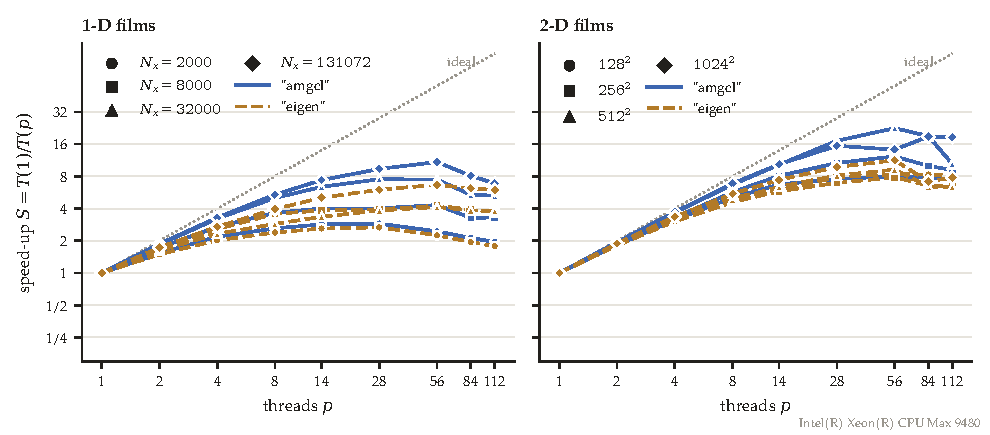
\includegraphics[width=\textwidth]{figures/parallel-scaling.pdf}
  \caption{The speed-up of \cref{tab:scaling} against the thread count, every
    size and both backends, with the ideal $S = p$ dotted. Both backends scale
    on the large films, \val{"amgcl"} further; the small 1-D film stops
    near $3\times$, and almost every case falls off past one socket (56
    threads). Drawn by \file{docs/manual/\bk figures/\bk make\_scaling.py} from
    \file{tools/scaling/\bk results/\bk scaling-mc076.tsv}.\label{fig:parallel-scaling}}
\end{figure}

\Cref{fig:parallel-scaling} shows the same numbers as curves. Four readings.

\paragraph{Both backends scale, \val{"amgcl"} further.}
At 56 threads \val{"eigen"} reaches $8\times$ to $11\times$ in 2-D and
\val{"amgcl"} $8\times$ to $22\times$, the larger factors on the larger films.
\val{"eigen"}'s preconditioner is a block-Jacobi ILUT whose blocks are
factorized in parallel (\cref{sec:linsolve:eigen}); what limits it is the
BiCGStab iterations, 33 to \SI{72}{\percent} of the loop, whose vector work is
sequential (\cref{sec:parallel:profile}). AMGCL threads its set-up and its
iterations alike.

\paragraph{Which backend is faster depends on the thread count.}
In 1-D the two are level at $N_x = 2000$, where AMGCL solves the system
directly (within \SI{9}{\percent} on one thread and \SI{2}{\percent} at 28),
and \val{"eigen"} is ahead at every thread count from $8000$ to $32000$:
$5.8\times$ on one thread and $5.7\times$ at 56 at $N_x = 8000$. AMGCL has
little to coarsen on a one-dimensional problem and needs about 100 linear
iterations a solve there, where Eigen needs 12. At $N_x = 131072$ the two are
within \SI{11}{\percent} on one thread and \val{"amgcl"} is $1.5\times$ faster at 56. In 2-D the
two are level at $128^2$; from $256^2$ up \val{"eigen"} is faster on one
thread ($1.4\times$ at $256^2$, $1.6\times$ at $512^2$, $1.2\times$ at
$1024^2$) and on eight threads up to $512^2$, and \val{"amgcl"} from 8 to 28
threads up ($1.1\times$ at 56 on $256^2$, $1.5\times$ on $512^2$,
$1.4\times$ at 28 on $1024^2$). \Cref{sec:parallel:backend} turns this into a
rule.

\paragraph{The useful thread count is 28--56, not 112.}
Every case but one is at or past its optimum by 56 threads and slower at 112
than at 56. The two sockets carry 8 NUMA nodes, and past one
socket the reductions and the memory traffic cost more than the extra cores
return; this is why a run uses at most one socket (\cref{sec:parallel:cap}).
The exception, \val{"amgcl"} on $1024^2$, is fastest at 84 threads, in
\SI{18}{\percent} less time than at 28; at 56 its three repeats spread by
\SI{22}{\percent}. (The \val{"amgcl"} row of $N_x = 2000$ was measured
again on another node of the same kind, after a fix to AMGCL's coarsest level;
\val{"eigen"} timed there agreed with \cref{tab:scaling} to \SI{2}{\percent}.)

\paragraph{Small problems do not parallelize.}
At $N_x = 2000$ the best speed-up is $2.7\times$ with \val{"eigen"} and
$2.9\times$ with \val{"amgcl"}, both at 28 threads, and past that more threads
cost time. Below a few thousand points,
run one thread per case and put several cases side by side. The kit that
measured \cref{tab:scaling} turns the thread limit off, so that every row is
the thread count asked for.

\begin{note}[Reading the Amdahl fit in the summary tool]
  \file{tools/scaling/summarize.py} prints a fitted parallel fraction $f$.
  Where a case slows down past its optimum the fit reports $f = 0.000$, which
  does not mean nothing is parallel: Amdahl's law can express saturation but
  not slowdown, so the regression has nothing to fit. Read $S$ and $E$,
  which are measured, in preference to $f$, which is a model.
\end{note}

\section{Which backend to ask for}
\label{sec:parallel:backend}

The measurements above give the following rule. The penalty for getting it
wrong is large only in 1-D; in 2-D the two backends are within a factor of
1.6 of each other at every size up to one socket of threads.

\begin{yzntable}{Backend by problem shape\label{tab:backend-rule}}{@{}L{0.22\textwidth} L{0.16\textwidth} L{0.50\textwidth}@{}}
\textsf{\bfseries Problem} & \textsf{\bfseries Backend} & \textsf{\bfseries Why}\\ \midrule
1-D, up to $\sim 10^4$--$10^5$ cells & \val{"eigen"} & AMGCL has almost nothing to coarsen and spends eight times the linear iterations: $5.7\times$ slower at $N_x=8000$. Level at $N_x = 2000$, where AMGCL solves directly. \\
1-D, $\sim 10^5$ cells and more & either & Within \SI{11}{\percent} on one thread; \val{"amgcl"} $1.5\times$ faster at 56 threads on $N_x = 131072$. \\
2-D, a socket of threads & \val{"amgcl"} & $1.1$--$1.5\times$ faster from $256^2$ up, level at $128^2$. \\
2-D, eight threads or fewer & \val{"eigen"} & Faster from $256^2$ up on one thread, by $1.2$--$1.6\times$. \\
\end{yzntable}

\val{"auto"} asks the film's in-plane dimension and returns \val{"eigen"} for
a 1-D film and \val{"amgcl"} for a 2-D one. The default is \val{"auto"}, so
leaving the key alone gives the faster backend in 1-D below $\sim 10^5$
cells and on a full socket in 2-D. On a small machine and a 2-D film of
$256^2$ or more, set \key{Backend} to \val{"eigen"}.

\begin{note}[Why there is no size or thread threshold]
  Where one backend overtakes the other depends on the machine, and outside
  1-D the gain is small either way. A threshold would put a machine-dependent
  guess into the solver, so \val{"auto"} splits on the dimension alone. If the
  run time of a long study matters, measure both on your machine
  (\cref{sec:parallel:kit}) and set \key{Backend} explicitly.
\end{note}

\section{Measuring it on your own machine}
\label{sec:parallel:kit}

\file{tools/scaling/} is a self-contained kit for exactly this measurement:
generated cases, a sweep script, and a summarizer.

\begin{shell}
cmake -S . -B build -DCMAKE_BUILD_TYPE=Release -DYUZEN_WITH_AMGCL=ON
cmake --build build -j

tools/scaling/scaling.sh --tier quick --repeats 1 --threads "1 4"
tools/scaling/scaling.sh --threads "1 2 4 8 16 32 64" --repeats 3
python3 tools/scaling/summarize.py tools/scaling/results/scaling-*.tsv
\end{shell}

The sweep appends one row per run to a tab-separated file that carries the
machine's identity in its header, and it skips rows it already has, so an
interrupted sweep is restarted by repeating the command. What makes the
numbers comparable is that the cases fix the work: the time step is constant
(\key{Numerics.TimeStepControl} disabled), the step count is fixed
(\key{Numerics.MaxSteps}), and field output is off --- the output interval
also caps the time step, so leaving it on would change the work per step as
well as the time spent writing. What is timed is the time-step loop alone,
taken from \file{JobInfo.txt}, not the whole process, so grid construction and
start-up do not dilute the result.

\begin{warn}[Small cases cannot use a large machine, whatever you do]
  The reductions in \code{Vector} are split into a fixed number of blocks,
  $\min(256,\,N/512)$ for $N$ elements, so that the answer does not depend on
  the thread count (\cref{sec:repro:reduction}). Two limits follow. A case
  with fewer than $512p$ unknowns cannot give all $p$ threads a block at all
  --- at 112 threads that is 57\,344 unknowns, and a comfortable margin needs
  131\,072 so that the block count reaches its ceiling. And because the
  ceiling is 256 blocks, \textbf{beyond 256 threads the reductions do not
  parallelize any further}. That ceiling is the price of bit-identity, and it
  is deliberate.

  This is why the kit's ladder goes up to $1024^{2}$ in 2-D and $N_x =
  131\,072$ in 1-D. The small cases are in it to show the other end: that they
  do not speed up, and should be run one thread each, several at a time.
\end{warn}

\subsection{Where the time goes}
\label{sec:parallel:profile}

With \env{YUZEN\_PROFILE=1} the solver times named parts of the run and
writes the totals to standard error at exit, one line each (name, calls,
seconds):
\begin{shell}
[profile] threads 8
[profile] h.linsolve        2030      0.097730
\end{shell}
\begin{yzntable}{The parts \env{YUZEN\_PROFILE} times. Times of nested parts are each inclusive: \code{h.linsolve} contains the \code{lin.*} of the film height.\label{tab:profile-parts}}{@{}L{0.20\textwidth} L{0.72\textwidth}@{}}
\textsf{\bfseries Name} & \textsf{\bfseries What}\\ \midrule
\code{step}        & one time step, all of it \\
\code{output}      & the field and history output between steps \\
\code{h.assemble}  & the film-height matrix (\code{SetMatrixA}) \\
\code{h.jacobian}  & its Jacobian and the matrix of the implicit step \\
\code{h.rhs}       & the explicit part and the right-hand side \\
\code{h.linsolve}  & the linear solve of the film height \\
\code{h.couple}    & the rest of a Newton pass, the well-mixed concentration trial among it \\
\code{h.after}     & the end of the step, the concentration of the step among it \\
\code{c.solve}     & a concentration solve, all of it; \code{c.linsolve} its linear solve \\
\code{velocity}    & the velocities \\
\code{lin.prepare} & handing the matrix to the backend: gathering, scaling, copying \\
\code{lin.precond} & building the preconditioner (ILUT factorization, AMG set-up) \\
\code{lin.iterate} & the BiCGStab iterations \\
\end{yzntable}
A scope inside a parallel region times nothing; what is timed is what the
thread running the time loop sees. \file{tools/profile\_threads.py} runs a
set of cases with both backends at each thread count, with the cap of
\cref{sec:parallel:cap} off, and tabulates the parts against the thread count;
it measures in pieces under a batch time limit as
\file{tools/case\_runtimes.py} does (\cref{sec:env:tools}).

On a Xeon Max 9480 node like that of \cref{tab:scaling} it shows where the limits of
\cref{sec:parallel:scaling} come from. With \val{"eigen"} on the 2-D films of
\cref{tab:scaling}, building the block-Jacobi ILUT preconditioner takes 6--30\,\%
of the time-step loop, the larger shares on the smaller grids, and the BiCGStab
iterations 33--72\,\%, the larger shares on the larger grids; on the $60\times60$
film of \file{leveling\_2d\_reg} the factorization takes 55--61\,\%, because its
blocks stop dividing the work at four threads. With \val{"amgcl"}, the AMG set-up
is rebuilt at every linear solve, five to eight times a step (about three
for the film height, two to four for the concentration), and it scales less well than the
iterations: its share of the loop grows from 4--9\,\% on one
thread to 10--28\,\% at 56, the larger
shares on the smaller grids. Handing the matrix to the backend takes
0--3\,\% on the 2-D cases at every thread count.

\section{Speed and reproducibility are separate questions}
\label{sec:parallel:repro}

Changing the thread count does not change the answer. With \val{"eigen"} the
result is bit-identical, and the test suite asserts it
(\cref{ch:reproducibility}); with \val{"amgcl"} it moves in the last few digits
(\cref{sec:verification:amgclthreads}). So the choice of thread count is purely
a performance decision, and the choice of backend is the one that has a
correctness dimension to it. If you need bit-identical results across machines
as well as across thread counts, fix the backend to \val{"eigen"} and accept
the slower 2-D solve.


\part{Theory}
% ch-governing.tex -- theory: the long-wave equations, their scaling and their limits
\chapter{The governing equations}
\label{ch:governing}

This chapter states what Yuzen actually solves: one evolution equation for the
film thickness, one transport equation for the solute, the approximation that
reduces the Navier--Stokes equations to them, and the scaling that turns them
into the dimensionless form the solver works in. Read it if you want to know
what a given input key does to the mathematics, or where the model stops being
trustworthy. The individual flux terms are taken one at a time in
\cref{ch:terms}; the keys themselves are in \cref{ch:ref-physics,ch:ref-domain}.

\section{The long-wave approximation}
\label{sec:governing:longwave}

When the film thickness $h$ is small compared with the representative in-plane
length $L$, the Navier--Stokes equations collapse into a single evolution
equation for $h(x,y,t)$. This is the long-wave --- or lubrication ---
approximation, and it is the equation Yuzen solves. Four assumptions go into
it, and each of them buys something and costs something.

\begin{itemize}
  \item \textbf{The aspect ratio is small}, $\varepsilon = h_0/L_0 \ll 1$. This
    is what allows the cross-film coordinate to be eliminated altogether: you
    solve a problem in one or two dimensions instead of two or three, and the
    unknown is a surface rather than a volume. The cost is that every
    conclusion is an expansion in $\varepsilon$, so nothing the model says
    about a feature as short as the film is thick can be believed.
  \item \textbf{Inertia is negligible.} The velocity profile across the film is
    then exactly parabolic, with no slip at the substrate (or a Navier slip
    length, \key{Physics.Slip}: \cref{sec:terms:slip}) and a shear stress at
    the free surface set solely by the surface-tension gradient. This is what
    makes the depth-integrated flux $\Qvec$ an explicit algebraic function of
    $h$ and the driving pressures, with no momentum equation left to solve. The
    cost is that fast rotation and low-viscosity films, where the profile
    departs from the parabola, are outside the model.
  \item \textbf{The pressure is uniform across the film.} Capillary pressure,
    gravity and disjoining pressure all enter one single pressure. This is what
    lets every physical effect be added as one more term in the same bracket,
    and it is why switching a term off is a matter of zeroing a coefficient
    rather than changing the equation. The cost is that no effect with
    structure through the thickness --- a pressure that varies with depth ---
    can be represented at all.
  \item \textbf{The interface slope is small}, so the curvature may be
    linearized to $\nabla^2 h$; that is, the denominator of the exact mean
    curvature $\nabla\cdot\bigl(\nabla h/\sqrt{1+|\nabla h|^2}\bigr)$ is set to
    1. This is what keeps the capillary term linear in the highest derivative
    and the whole equation tractable. The cost is a direct error wherever the
    surface is steep, which is exactly where a contact line is; see
    \cref{sec:governing:breakdown}.
\end{itemize}

\section{The dimensional equations}
\label{sec:governing:dimensional}

In dimensional variables the film thickness obeys

\begin{equation}\label{eq:height-dim}
  \frac{\partial h}{\partial t} = -\nabla\cdot\Qvec \;-\; E(h,c) \;+\; S(x,t),
\end{equation}

where $\Qvec$ is the flux integrated across the thickness, $E$ is the rate at
which evaporation removes thickness, and $S$ is liquid supplied from a nozzle.
The flux collects six contributions:

\begin{equation}\label{eq:flux-dim}
  \begin{aligned}
    \Qvec = {}& \frac{\sigma h^{3}}{3\mu}\,\nabla\nabla^{2}(h+s)
      && \text{capillary pressure} \\
      &{}- \frac{\rho g_z h^{3}}{3\mu}\,\nabla(h+s)
      && \text{vertical gravity} \\
      &{}+ \frac{h^{3}}{3\mu}\,\nabla\Pi(h)
      && \text{disjoining pressure} \\
      &{}+ \frac{h^{2}}{2\mu}\,\nabla\sigma
      && \text{Marangoni stress} \\
      &{}+ \frac{\rho g_\parallel h^{3}}{3\mu}
      && \text{in-plane gravity} \\
      &{}+ \frac{\rho \omega^{2} h^{3}}{3\mu}\,r\,\er
      && \text{centrifugal force.}
  \end{aligned}
\end{equation}

Here $h$ is the film thickness and $s(x,y)$ is the height of the substrate, so
the free surface sits at $h+s$. The distinction matters and it is not
cosmetic. \textbf{Capillary pressure and vertical gravity are driven by the
shape of the free surface $h+s$}, because both are consequences of where the
liquid surface is in space; \textbf{disjoining pressure is a function of the
film thickness $h$ alone}, because it describes an interaction between the
substrate and the free surface whose strength depends only on how far apart
they are. One practical consequence is that a substrate shape does nothing
unless at least one of the first two terms is enabled
(\cref{sec:terms:vgravity}).

Both $\mu = \mu(c)$ and $\sigma = \sigma(c)$ depend on the solute
concentration (\cref{sec:conc:properties}), which is what couples
\cref{eq:height-dim} to the transport equation below.

\begin{note}[The velocity Yuzen writes out is not a new unknown]
  Nothing in \cref{eq:height-dim,eq:flux-dim} solves for a velocity. The
  in-plane velocity in the field output is the quantity $\Qvec/h$ --- the
  depth-averaged velocity implied by the flux, summed over the active terms.
  The \file{.vts} files of the well-mixed models also report it term by term,
  one array per contribution in \cref{eq:flux-dim} except the disjoining
  pressure (\cref{sec:output:vtk}). That decomposition is the most direct way
  to see which physical effect is actually moving the liquid at a given place
  and time.
\end{note}

\section{Solute transport}
\label{sec:governing:concentration}

The solute (resin) concentration $c$ is a mass fraction, so $c = 1$ means
completely dry. In the well-mixed model it is taken to be uniform across the
thickness, and what is conserved is the solute held in a column of the film,
$hc$:

\begin{equation}\label{eq:conc-dim}
  \frac{\partial (hc)}{\partial t} + \nabla\cdot\bigl(c\,\Qvec\bigr)
    = \nabla\cdot\bigl(D(c)\,h\,\nabla c\bigr) \;+\; c_S\,S .
\end{equation}

The solute is carried by the same flux $\Qvec$ that moves the liquid in
\cref{eq:height-dim}, spreads by diffusion along the film, and arrives with the
liquid a nozzle supplies. $c_S$ is the concentration that liquid arrives at,
chosen by \key{Physics.Source.ConcType} (\cref{sec:terms:source}): $c_S = c$,
the concentration already present where it lands (\val{"local"}, the
default), or $c_S = \key{Physics.Source.Conc}$ (\val{"supplied"}), mixed
through the thickness of the column it lands on. \textbf{Evaporation does not appear}: it removes
solvent and leaves the solute behind. This is the equation Yuzen evolves ---
the unknown it advances is the solute $hc$ of each cell, with the film $h$ of
the same step --- so the solute of a closed film is conserved to rounding and a
uniform $c$ stays uniform whatever the film does, unless liquid of another
concentration is supplied (\cref{sec:disc:wm-conservative}).

Subtracting $c$ times \cref{eq:height-dim} gives the same law for $c$ itself,
with $\uvec = \Qvec/h$ the mixed velocity of all the enabled terms:
%
\begin{equation}\label{eq:conc-adv}
  \frac{\partial c}{\partial t} + \uvec\cdot\nabla c
    = \frac{1}{h}\,\nabla\cdot\bigl(D(c)\,h\,\nabla c\bigr)
      \;+\; \frac{E c}{h} \;+\; \frac{S\,(c_S - c)}{h}.
\end{equation}

It is the clearer form to read, and its evaporation term is the one that makes drying
interesting. Evaporation removes
solvent but not solute, so whatever is left behind becomes more concentrated;
the rate at which it does so is the thickness lost per unit time, $E$, divided
by the thickness that is there to dilute it, $h$. \textbf{Because it is divided
by $h$, concentration rises fastest where the film is thinnest.} That is the
mechanism behind edge effects in a drying coating, and it is also why a
contact-line calculation needs the precursor-film correction of
\cref{sec:terms:evaporation}: without it, the thinnest region in the domain
would dry out first and fastest. The last term is the nozzle's, and it is 0
when the liquid arrives at the local concentration; liquid supplied at
another $c_S$ pulls $c$ toward $c_S$ at the rate $S/h$, so a thin film under
the nozzle takes on the supplied concentration quickly and a thick one slowly.

If you need the distribution of concentration through the thickness rather than
a depth average, use the \val{"CZ"} model instead (\cref{sec:conc:cz}).

\section{Where the assumptions break down}
\label{sec:governing:breakdown}

\paragraph{Large slope.} Two separate errors appear together. The linearized
curvature loses accuracy, and so does the small-angle substitution
$1-\cos\thetae \approx \thetae^{2}/2$ used to calibrate the disjoining pressure
(\cref{sec:wetting:dp}). The second error is easy to quantify exactly:

\begin{yzntable}{Error of $1-\cos\thetae \approx \thetae^{2}/2$\label{tab:cos-error}}{@{}d d@{}}
\textsf{\bfseries $\thetae$ [deg]} & \textsf{\bfseries error} \\ \midrule
10 & 0.3 \% \\
20 & 1.0 \% \\
30 & 2.3 \% \\
45 & 5.3 \% \\
90 & 23 \% \\
\end{yzntable}

\key{Physics.DisjoiningPressure.ContactAngle} accepts anything in $[0:90]$
degrees, but if you intend to use the angle quantitatively, keep it small.

\paragraph{Inertia.} At high rotation rates, or in a low-viscosity film, the
velocity profile departs from the parabola the derivation assumes. Nothing in
the solver detects this; the equations remain perfectly well behaved and simply
describe a different problem from the one you have.

\paragraph{In-plane lengths approaching the film thickness.} The
neighborhood of a contact line is by construction a region of large slope and
short in-plane length --- the two things the approximation is least able to
handle. The disjoining pressure is the device that lets the long-wave equation
be carried into that region at all, and \cref{ch:wetting} is about what it can
and cannot deliver there.

All of this is concentrated in one number. The assumption that the film is thin
appears in the dimensionless group

\[
  \As = \left(\frac{L_0}{h_0}\right)^{2},
\]

and a configuration in which $\As$ falls toward order 1 is outside the range
of the approximation altogether.

\section{Scales}
\label{sec:governing:scales}

Every value in the input file is dimensional --- meters, seconds, pascal
seconds --- but the solver works entirely in dimensionless variables. Five
scales do the conversion.

\begin{yzntable}{The scales used for non-dimensionalization\label{tab:scales}}{@{}l L{0.42\textwidth} L{0.44\textwidth}@{}}
\textsf{\bfseries Symbol} & \textsf{\bfseries What it is} &
\textsf{\bfseries Set by} \\ \midrule
$L_0$ & In-plane length: the capillary length $\sqrt{\sigma_0/(\rho g)}$, with $g = \SI{9.80665}{\metre\per\second\squared}$ & \key{LengthScaleType}; with \val{"custom"}, $L_0$ is taken from \key{LengthScale} instead \\
$h_0$ & Film thickness & \key{Initial.SurfaceShape.TotalHeight} \\
$T_0$ & Time, $\mu_0 L_0^{4}/(\sigma_0 h_0^{3})$ & follows from $\mu_0$, $\sigma_0$, $L_0$ and $h_0$ \\
$U_0$ & Velocity, $L_0/T_0$ & follows from $L_0$ and $T_0$ \\
$\varepsilon$ & Aspect ratio, $h_0/L_0$ & follows from $h_0$ and $L_0$ \\
\end{yzntable}

The reference properties are $\sigma_0 =$ \key{Fluid.SurfaceTension.BaseValue},
$\rho =$ \key{Fluid.Density.Value} and $\mu_0 =$
\key{Fluid.Viscosity.BaseValue}. Writing \key{LengthScaleType = "custom"}
replaces the capillary length by whatever \key{LengthScale} says.

The dimensionless thickness is $H = h/h_0$ and the dimensionless in-plane
coordinate is $X = x/L_0$. It follows that

\begin{equation}\label{eq:slope-conversion}
  \text{physical slope} \;=\; \varepsilon \times \text{dimensionless slope},
\end{equation}

and \cref{eq:slope-conversion} is not a footnote: \textbf{the entire discussion
of contact angles in \cref{ch:wetting} rests on it}. A dimensionless profile
that rises by 1 over a unit of $X$ is a physical surface inclined at
$\varepsilon$, not at $45^\circ$. Four of the five --- $L_0$, $h_0$, $T_0$ and
$U_0$ --- are printed in the run log on standard output under the heading
\code{Scaling factors} (\cref{sec:output:running}); read them rather than
recomputing them. $\varepsilon$ is not printed, but it is $h_0/L_0$ of the two
that are.

\section{The dimensionless groups}
\label{sec:governing:groups}

Twelve dimensionless groups carry the whole of the input into the equations.

\begin{yzntable}{The dimensionless groups\label{tab:groups}}{@{}l L{0.225\textwidth} L{0.22\textwidth} L{0.375\textwidth}@{}}
\textsf{\bfseries Symbol} & \textsf{\bfseries Definition} &
\textsf{\bfseries Meaning} & \textsf{\bfseries Set by} \\ \midrule
$\As$   & $(L_0/h_0)^{2}$ & Inverse aspect ratio squared; the strength of capillary pressure & \key{Initial.SurfaceShape.TotalHeight} together with $L_0$ \\
$\Bo$   & $\rho g_z L_0^{2}/\sigma_0$ & Bond number; gravity normal to the substrate & \key{Physics.\bk VerticalGravity.\bk Acceleration} \\
$\Pgx$  & $\rho g_x L_0^{2}/(\sigma_0\varepsilon)$ & In-plane gravity along $x$; non-zero on a tilted substrate & \key{Physics.\bk HorizontalGravity.\bk Acceleration[0]} \\
$\Pgy$  & $\rho g_y L_0^{2}/(\sigma_0\varepsilon)$ & In-plane gravity along $y$ & \key{Physics.\bk HorizontalGravity.\bk Acceleration[1]} \\
$\Spn$  & $\rho \omega^{2} L_0^{4}/(\sigma_0 h_0)$ & Spin number; centrifugal force & \key{Physics.Centrifugal.RotationRate} \\
$\Ma$   & $(\mathrm{d}\sigma/\mathrm{d}c)/\sigma_0$ & Marangoni number; how strongly surface tension depends on concentration & \key{Fluid.SurfaceTension.Coef} \\
$\Dpn$  & $\displaystyle\frac{\As\,(n-1)(m-1)\,\thetae^{2}}{2\,\Hstar\,(n-m)}$ & Disjoining-pressure coefficient, fixed by the target equilibrium contact angle & \key{Physics.DisjoiningPressure.*} together with \key{PrecursorRatio} \\
$\Hstar$ & \key{PrecursorRatio} & Dimensionless precursor thickness; the root of $\Pihat(\Hstar) = 0$ & \key{Initial.SurfaceShape.PrecursorRatio} \\
$\Ev$   & $E_0 T_0/h_0$ & Evaporation number; how fast evaporation thins the film & \key{Physics.Evaporation.Coef} \\
$\Pen$  & $E_0 h_0/D_0$ & P\'eclet number; evaporation against cross-film diffusion & \key{Physics.Evaporation.Coef}, \key{Fluid.Diffusivity.BaseValue} \\
$\Df$   & $D_0 T_0/L_0^{2}$ & Diffusion number; the speed of in-plane diffusion & \key{Fluid.Diffusivity.BaseValue} \\
$\Mr$   & $M_{\mathrm{resin}}/M_{\mathrm{solvent}}$ & Molar-mass ratio, used by Raoult's law & \key{Fluid.MolarMass.Solvent}, \key{Fluid.MolarMass.Resin} \\
$\Lambda$ & $\lambda/h_0$ & Dimensionless slip length; mobility $H^3/3 + \Lambda H^2$ (\cref{sec:terms:slip}) & \key{Physics.Slip.Length} \\
\end{yzntable}

In these definitions $g_z$, $g_x$ and $g_y$ are the components of gravitational
acceleration given in the input in \si{\metre\per\second\squared}, $\omega$ is
the rotation rate in \si{\radian\per\second}, $E_0$ is the evaporation
coefficient in \si{\metre\per\second} and $D_0$ is the reference diffusivity in
\si{\metre\squared\per\second}.

$\Bo$, $\Pgx$, $\Pgy$, $\Spn$, $\Ma$ and $\Dpn$ are \textbf{set to zero} when
the corresponding term is disabled in the input, and the term is then not
assembled at all (\cref{sec:repro:order}). $\Ev$, $\Pen$ and $\Df$ always carry a value, and evaporation and
diffusion are switched on and off by separate keys instead. Note the
side-effect of the first rule: $\Ma = 0$ removes the Marangoni stress and, at
the same time, removes the concentration dependence of surface tension entirely
(\cref{sec:conc:properties}).

One number is worth remembering. If you leave the length scale at the capillary
length and set \key{Acceleration = 9.80665} --- that is,
$g = \SI{9.80665}{\metre\per\second\squared}$ --- then $\Bo = 1$ exactly, since
the capillary length is defined as the length at which gravity and surface
tension balance. \key{Acceleration} is therefore the key to change when you want to
move $\Bo$.

\section{The dimensionless equations}
\label{sec:governing:nondim}

With those scales and groups, \cref{eq:height-dim,eq:flux-dim} become

\begin{equation}\label{eq:height}
  \frac{\partial H}{\partial T} = -\nabla\cdot\Qvec - \Ev\,\hat{E}(H,C) + \hat{S},
\end{equation}

\begin{equation}\label{eq:flux}
  \Qvec = \frac{H^{3}}{3\hat{\mu}}
    \Bigl[\,\hat{\sigma}\,\nabla\nabla^{2}(H+S)
      - \Bo\,\nabla(H+S)
      + \Dpn\,\nabla\Pihat(H)
      + \Pvec
      + \Spn\,r\,\er \Bigr]
    + \frac{\As\,\Ma}{2}\,\frac{H^{2}}{\hat{\mu}}\,\nabla C,
\end{equation}

and the solute balance \cref{eq:conc-dim} becomes

\begin{equation}\label{eq:conc}
  \frac{\partial (HC)}{\partial T} + \nabla\cdot\bigl(C\,\Qvec\bigr)
    = \Df\,\nabla\cdot\bigl(\hat{D}(C)\,H\,\nabla C\bigr) + C_S\,\hat{S},
\end{equation}

with $C_S = c_S$ the concentration the supplied liquid arrives at ($C$ itself
by default), and the disjoining pressure

\begin{equation}\label{eq:pihat}
  \Pihat(H) = (\Hstar/H)^{n} - (\Hstar/H)^{m}.
\end{equation}

Here $\hat{\mu}(C)$, $\hat{\sigma}(C)$ and $\hat{D}(C)$ are the viscosity,
surface tension and diffusivity normalized to 1 at the reference concentration, and $\Pvec = (\Pgx, \Pgy)$.
Note that $S$ without a hat is the dimensionless substrate height, while
$\hat{S}$ with one is the dimensionless source; they are different quantities
that unfortunately share a letter.

The single most useful thing to notice in \cref{eq:flux} is what makes it
vanish. Five of the six contributions sit inside one bracket multiplied by
$H^{3}/3\hat{\mu}$, so $\Qvec = 0$ requires the contents of that bracket to be
\emph{uniform in space}. That statement --- uniformity of the bracket, not
smallness of any individual term --- is the equilibrium condition, and it is
where \cref{ch:wetting} starts. In the discretization, thickness and
concentration live at cell centers and velocities on cell faces
(\cref{ch:discretization}).

% ch-terms.tex -- theory: the individual physics terms of the flux
\chapter{The physics terms}
\label{ch:terms}

\Cref{eq:flux} collects six flux contributions, and \cref{eq:height} adds
evaporation and a source. Each of them has its own sub-block under
\key{Physics} and its own \key{Enable} key, so they are switched on and off one
at a time. This chapter takes them in turn: what the term is, what it does to
the film, what behavior you should expect to see when it dominates, and which
keys control it. The keys are quoted by name only --- their types, defaults and
ranges are tabulated once, in \cref{ch:ref-physics}, and are not repeated here.

\section{Capillary (Laplace) pressure}
\label{sec:terms:laplace}

\begin{equation}\label{eq:q-cap}
  \Qvec_{\mathrm{cap}}
    = \frac{\hat{\sigma}(C)\,H^{3}}{3\hat{\mu}(C)}\,\nabla\nabla^{2}(H+S).
\end{equation}

Surface tension acting to flatten the free surface. It is responsible for
almost everything the word ``leveling'' covers: a rough coating smoothing
itself out, a drop relaxing toward a spherical cap, liquid collecting in the
dips of a textured substrate. In practice nearly every run keeps it on.

Two details are worth holding on to. First, \textbf{this term is why the height
equation is fourth order}: $\nabla\nabla^{2}$ is three derivatives acting on
$H$ inside a divergence, so \cref{eq:height} carries a fourth spatial
derivative, and that in turn is why each boundary needs two conditions
(\cref{sec:conc:boundaries}) and why the linear systems are what they are
(\cref{ch:linearsolver}). Second, the curvature is measured on the free surface
$H+S$, not on the film thickness $H$ --- which is how the substrate shape gets
into the problem at all.

Its mobility contains $\hat{\sigma}(C)$ as well as $\hat{\mu}(C)$, so as a film
dries and its surface tension changes, the rate at which it levels changes too.

The only key is \key{Physics.LaplacePressure.Enable}
(\cref{sec:ref-physics:laplace}).

\section{Disjoining pressure}
\label{sec:terms:disjoining}

\begin{equation}\label{eq:q-dis}
  \Qvec_{\mathrm{dis}} = \Dpn\,\frac{H^{3}}{3\hat{\mu}}\,\nabla\Pihat(H),
  \qquad
  \Pihat = (\Hstar/H)^{n} - (\Hstar/H)^{m},
  \qquad n > m > 1.
\end{equation}

Once a film becomes very thin, the substrate and the free surface start to
interact with one another. Expressing that interaction as a pressure gives the
disjoining pressure, and it is this term that gives the model partial wetting:
a finite contact angle and a contact line that can move. The first term of
$\Pihat$ is repulsive and tries to keep the film thick; the second is
attractive. They cancel at $H = \Hstar$, where $\Pihat = 0$, and that thickness
is the precursor film left behind outside a drop.

The characteristic behavior is a drop of finite extent sitting on a thin
precursor, with a transition region between the two whose width is set by
$\Hstar$ and the contact angle. How the coefficient $\Dpn$ is calibrated
against the angle you ask for, and how wide that transition region actually is,
is the subject of \cref{ch:wetting}.

Four keys live in the \key{Physics.DisjoiningPressure} block: \key{Enable},
\key{ContactAngle}, \key{ExponentN} and \key{ExponentM}. The precursor
thickness comes from \key{Initial.SurfaceShape.PrecursorRatio}
(\cref{sec:ref-physics:disjoining}). Enabling the term with
\key{PrecursorRatio} left at \val{0} leaves $\Hstar$ undefined and terminates
the run.

\begin{warn}[This is the stiffest term in the model]
  $\Pihat \sim H^{-n}$ is a very strong non-linearity: with the conventional
  exponents $(n,m) = (3,2)$ a halving of the thickness multiplies the repulsive
  branch by 8. They are the defaults of \key{ExponentN} and \key{ExponentM}
  (\cref{sec:ref-physics:disjoining}).
  Nothing else in the equation responds that steeply to a small change in $H$.
  Expect this term to dominate the Newton iteration, the conditioning of the
  linear system and the admissible time step whenever it is on.
\end{warn}

\section{Vertical gravity and the substrate shape}
\label{sec:terms:vgravity}

\begin{equation}\label{eq:q-vg}
  \Qvec_{\mathrm{vg}} = -\frac{\Bo}{3}\,\frac{H^{3}}{\hat{\mu}}\,\nabla(H+S).
\end{equation}

Gravity normal to the substrate. Hydrostatic pressure drives liquid from the
high parts of the free surface to the low ones, so on a horizontal substrate it
flattens bumps and works alongside capillary pressure; the two together are
what level a film. The difference between them is the order of the derivative,
and hence the length scale: gravity levels long-wavelength unevenness that
capillary pressure barely feels.

The keys are \key{Physics.VerticalGravity.Enable} and
\key{Physics.\bk VerticalGravity.\bk Acceleration}, the latter in
\si{\metre\per\second\squared} (\cref{sec:ref-physics:vgravity}). If you are
using a substrate tilted by an angle $\alpha$, the value to give here is
$g\cos\alpha$, and the in-plane component goes to
\cref{sec:terms:hgravity}.

\subsection*{The substrate shape}

The substrate profile $S(x,y)$ is built in the \key{Substrate} block. Any
number of \key{RectBump}, \key{EllipseBump}, \key{PeriodicWave},
\key{FlatPlane}, \key{MexicanHat} and \key{SmoothConvex} blocks may be listed;
they are applied in ascending \key{Order} and combined into one shape
(\cref{sec:ref-domain:substrate}). The substrate never moves and never changes
with time.

$S$ enters the equations only through the combination $H+S$, and only in
\cref{eq:q-cap,eq:q-vg}. \textbf{If neither capillary pressure nor vertical
gravity is enabled, the substrate shape does nothing whatsoever} --- it is
parsed, built, written to the output and then never read by any term. This is
a common way to spend an afternoon wondering why a carefully built topography
has no effect.

\section{In-plane gravity}
\label{sec:terms:hgravity}

\begin{equation}\label{eq:q-hg}
  \Qvec_{\mathrm{hg}} = \frac{\Pvec}{3}\,\frac{H^{3}}{\hat{\mu}}.
\end{equation}

Flow down an inclined substrate. What distinguishes it from vertical gravity is
that the driving field is a constant vector, independent of position: there is
no gradient in it at all. The flux is then simply proportional to $H^{3}$, so
\textbf{thicker parts of the film run faster}, the thick regions overtake the
thin ones, and a front forms at the leading edge. That front steepening is the
signature behavior of this term, and it is the origin of the fingering
instabilities seen in real coatings running downhill.

The keys are \key{Physics.HorizontalGravity.Enable} and
\key{Physics.\bk HorizontalGravity.\bk Acceleration}, a pair $(g_x, g_y)$ in
\si{\metre\per\second\squared} (\cref{sec:ref-physics:hgravity}). For a
substrate tilted by $\alpha$, give the in-plane component $g\sin\alpha$ ---
\num{4.903} at $30^\circ$. The sign sets the downhill direction.

\section{Centrifugal force}
\label{sec:terms:centrifugal}

\begin{equation}\label{eq:q-cf}
  \Qvec_{\mathrm{cf}} = \frac{\Spn}{3}\,\frac{H^{3}}{\hat{\mu}}\,r\,\er.
\end{equation}

A rotating substrate throws the film outwards. This is the main driving force
of spin coating. The driving field is proportional to the distance $r$ from the
rotation axis, so unlike in-plane gravity it is not uniform: the effect is
weak at the center and strongest at the rim, which is what produces the
characteristic thinning-from-the-middle history of a spin-coated film.

The keys are \key{Physics.Centrifugal.Enable},
\key{Physics.Centrifugal.RotationRate} in \si{\radian\per\second}, and
\key{Physics.Centrifugal.RotationAxis}, the coordinates of the rotation center
in meters (\cref{sec:ref-physics:centrifugal}).

\begin{note}[What a 1-D spin-coating run does with the $y$ direction]
  In a \val{"xh"} run there is no $y$ direction to be thrown into, but the
  liquid would be thrown there all the same. The solver accounts for it: the
  material that would leave through the unsolved $y$ direction is treated as
  loss, $\partial_y[\tfrac13\mathrm{Sp}\,H^3(y-y_0)/\hat\mu] = \tfrac13\mathrm{Sp}\,H^3/\hat\mu$
  --- the line $y = y_0$ of a film that is uniform in $y$ there. A 1-D
  spin-coating run is therefore not a slice through a 2-D one, and its total
  volume falls even between walls. Both models do this; \val{"CZ"} also
  carries the sideways divergence into its vertical velocity. What leaves this
  way is counted as outflow in \file{History.dat} (\code{OutflowedVol},
  \code{OutflowedResin}), so \code{VolErr} still balances
  (\cref{sec:output:history}).
\end{note}

A rotating film is not periodic: the arm $r$ grows across the domain and jumps
by its length across a periodic seam, where liquid would be created or lost.
The solver refuses \val{"Periodic"} edges with the centrifugal term
(\cref{sec:ref-bcout:boundary}); a strip of a film that goes on beyond the domain
takes an \val{"Outlet"} at each end. The one exception is a run with a
manufactured solution (\key{Numerics.ManufacturedSolution}), whose source is
formed for the arm of each cell: the periodic domains of \file{tools/mms.py}
carry every term at once.

\section{Solutal capillarity (Marangoni)}
\label{sec:terms:marangoni}

\begin{equation}\label{eq:q-sc}
  \Qvec_{\mathrm{sc}} = \frac{\As\,\Ma}{2}\,\frac{H^{2}}{\hat{\mu}}\,\nabla C.
\end{equation}

A surface stress arising because surface tension depends on concentration.
Where drying is faster the concentration rises, surface tension changes with
it, and the resulting gradient drags liquid along the free surface. Drying
mottle and flow streaks in a coating commonly start here.

Note the power of $H$. \textbf{This term scales with $H^{2}$, not $H^{3}$,
because it is a shear applied at the surface rather than a body force acting
through the whole thickness.} Integrating a constant body force across a
parabolic profile gives $H^{3}/3$; integrating the response to a surface
traction gives $H^{2}/2$. One consequence is that Marangoni flow becomes
relatively more important as a film thins, which is precisely when
concentration gradients are strongest.

The keys are \key{Physics.SolutoCapillarity.Enable} and
\key{Fluid.SurfaceTension.Coef}, which is $\mathrm{d}\sigma/\mathrm{d}c$ in
\si{\newton\per\metre} per unit concentration
(\cref{sec:ref-physics:soluto}). The sign of \key{Coef} decides which way the
liquid is pulled. Setting \key{Enable = false} forces $\Ma = 0$, which removes
this term and, in the same stroke, removes the concentration dependence of
surface tension everywhere else (\cref{sec:conc:properties}).

\section{Navier slip at the substrate}
\label{sec:terms:slip}

Slip is not a term of its own but a change of every mobility. With a slip
length $\lambda$ the velocity at the substrate is $\lambda\,\partial u/\partial z$
instead of zero, the parabolic profile gains a uniform slip velocity, and the
flux integrated across the film becomes
%
\begin{equation}\label{eq:q-slip}
  \Qvec = -\frac{1}{\mu}\Big(\frac{h^{3}}{3} + \lambda h^{2}\Big)\nabla p
          + \frac{1}{\mu}\Big(\frac{h^{2}}{2} + \lambda h\Big)\nabla\sigma .
\end{equation}
%
In the dimensionless equations $H^{3}/3$ of \cref{eq:q-cap,eq:q-dis,eq:q-vg,eq:q-hg,eq:q-cf}
becomes $H^{3}/3 + \Lambda H^{2}$ and $H^{2}$ of \cref{eq:q-sc}
becomes $H^{2} + 2\Lambda H$, with $\Lambda = \lambda/h_0$. The extra part grows
relative to the no-slip one as the film thins, $3\Lambda/H$ against 1: slip
matters most at a contact line, where it relieves the stress singularity as a
precursor film does by other means. It leaves the driving potential, and
therefore every equilibrium, unchanged. The keys are in
\cref{sec:ref-physics:slip}; the well-mixed model only.

\section{Evaporation}
\label{sec:terms:evaporation}

Evaporation is not a flux contribution. It removes solvent only, so it enters
the film-height equation and not the balance of the solute:

\begin{yzntable}{Where the evaporation rate enters\label{tab:evap-terms}}{@{}l L{0.5\textwidth}@{}}
\textsf{\bfseries Equation} & \textsf{\bfseries Evaporation term} \\ \midrule
Height, \cref{eq:height} & $-\Ev\,\hat{E}(H,C)$ \\
Solute $HC$, \cref{eq:conc} & none \\
Concentration $C$, the form of \cref{eq:conc-adv} & $+\Ev\,\hat{E}(H,C)\,C/H$ \\
\end{yzntable}

The film thins and the solute left behind becomes more concentrated. Written for
$C$, the enrichment is divided by $H$, so thin regions concentrate fastest ---
the same observation made about \cref{eq:conc-adv}.

The rate factorizes into three independent pieces, plus a correction:

\begin{equation}\label{eq:evap-factor}
  \hat{E} = \mathrm{Coef}\cdot f_{\mathrm{conc}}(C)\cdot
            f_{\mathrm{space}}(X)\cdot f_h(H).
\end{equation}

\begin{description}
  \item[Concentration, $f_{\mathrm{conc}}$] chosen by \key{ConcFunc}.
    \val{"Raoult"} is Raoult's law: the rate is proportional to the mole
    fraction of solvent, computed from the molar-mass ratio $\Mr$ of
    \key{Fluid.MolarMass}. \val{"PowerN"} is
    $(1 - C - \mathrm{ConcR})^{\mathrm{PowerN}}$, floored at zero so it never
    goes negative.
  \item[Position, $f_{\mathrm{space}}$] chosen by \key{SpatialFunc}.
    \val{"uniform"} is the same everywhere in the plane. \val{"negPow"} is a
    power of the distance to the rim of a circular pool of radius
    $R = \mathrm{NegPowRmax}$ centered on the origin of the grid coordinates,
    \begin{equation}\label{eq:evap-negpow}
      f_{\mathrm{space}} = \min\!\Bigl(k\,\bigl(1 - r/R'\bigr)^{-n},\ 10\Bigr),
      \qquad k = \tfrac{1}{2}(1-n)(2-n),\quad R' = 1.001\,R,
    \end{equation}
    with $r = \sqrt{x^2+y^2}$ and $n = \mathrm{NegPowExponent} < 1$; $k$
    makes the mean over the disc $r < R'$ equal to 1, which needs $n < 1$.
    For $0 < n < 1$ the rate diverges toward the rim, capped at 10; $n = 0$
    is uniform, and for $n < 0$ the rate falls to zero at the rim. Over the last 5 cells before $R$ the curve is blended
    into a quarter cosine that takes over its value and slope and levels off
    at $R$, and the rate is constant beyond $R$.
  \item[Precursor correction, $f_h$] a correction that suppresses evaporation
    from the precursor film. It is applied only when \key{PrecursorRatio} is
    greater than zero, and it ramps up linearly: \textbf{zero at $H = \Hstar$,
    and 1 at $H = 20\Hstar$.} It is zero below $\Hstar$ as well, so a film
    thinner than the precursor neither evaporates nor takes up solvent. Its purpose is to stop the precursor drying out
    and disappearing, so it is always active in a calculation that contains a
    contact line.
\end{description}

No step removes more solvent than the film holds: $E\Delta t \le h(1-c)$, at
either end of the step and in both equations, beside the cap at
$h/(2\Delta t)$. A film therefore dries toward $c = 1$ without passing it ---
with a rate that does not depend on $c$, a third of the remaining solvent is
left after each step --- and no solute is ever removed. Raoult's law takes $c$
within $[0, 1]$.

\key{Physics.Evaporation.Coef} has the dimensions of a velocity,
\si{\metre\per\second}, and is the source of both $\Ev$ and $\Pen$ --- changing
it moves the balance against diffusion as well as the drying rate. The
condition under which a run is declared dry and stopped is set by
\key{EndConcType} (\val{"mean"}, \val{"max"} or \val{"min"}) and
\key{EndConcValue}. All of these keys are tabulated in
\cref{sec:ref-physics:evaporation}.

\section{The source (nozzle)}
\label{sec:terms:source}

The supply term $\hat{S}$ added to \cref{eq:height}. It is modeled as a nozzle
mounted on the end of a rotating arm dispensing liquid onto the film, which
covers both a stationary dispense and a moving one. The keys live in
\key{Physics.Source} (\cref{sec:ref-physics:source}).

\begin{description}
  \item[Footprint] \key{Radius} is the radius of the nozzle mouth in meters. A
    cell receives supply in proportion to the fraction of it covered by that
    circle --- by that interval, in 1-D. \key{SubRegions} sets how many
    sub-divisions per cell are used to measure the fraction, so a larger value
    makes the supply vary more smoothly as the nozzle moves. Each
    sub-division counts when its center lies inside the footprint.
  \item[Rate] \key{InletRate} is the steady-state supply, given with the
    dimensions of a rate of thickness increase, \si{\metre\per\second}.
    \key{TimeConstant} is the rise-time constant $\tau$ in seconds, with the
    rate growing as $1 - e^{-t/\tau}$.
  \item[Arm] \key{ArmCenter} is the pivot position in meters and
    \key{ArmLength} the arm length, also in meters; \key{RotationRate} is its
    angular velocity in \si{\radian\per\second} and \key{StartAngle} the
    initial angle in radians.
    \key{ArmLength = 0} gives a nozzle that does not move. \key{RampTime} and
    \key{PlateauTime} are the ramp time applied to the rotation rate and the time
    it holds its plateau: the rate is $\omega f(t)$, with $f$ rising linearly
    from 0 to 1 over $T_s$, holding 1 for $T_m$ and falling back to 0 over
    another $T_s$, and the arm's angle is
    $\theta = \theta_0 + \omega\int_0^t f\,dt'$, so the arm stops at
    $\theta_0 + \omega(T_s + T_m)$ and stays there.
\end{description}

\paragraph{The concentration of the supplied liquid.}
\key{ConcType} says what the arriving liquid brings to the solute balance
\cref{eq:conc-dim}, as $c_S\,S$ (in the well-mixed model; \val{"CZ"} ignores
the nozzle altogether, \cref{sec:ref-physics:disjoining}):
\begin{description}
  \item[\val{"local"} (the default)] The liquid has the concentration already
    present where it lands, $c_S = c$. It thickens the film without changing
    $c$, and \key{Conc} is not used.
  \item[\val{"supplied"}] The liquid has the concentration \key{Conc}, a mass
    fraction in $[0:1]$, $c_S = \key{Conc}$. It is mixed through the
    thickness of the column it lands on, as the well-mixed model assumes of
    all its liquid, so the solute $hc$ of the column grows by $S\,c_S$ while
    its film grows by $S$. On a film that does not flow,
    \begin{equation}\label{eq:source-mixing}
      c(t) = \frac{h_0 c_0 + c_S\int_0^t S\,dt'}{h_0 + \int_0^t S\,dt'},
    \end{equation}
    so a thin film under the nozzle takes on $c_S$ quickly and a thick one
    slowly; in general the concentration is pulled toward $c_S$ at the rate
    $S/h$ (\cref{eq:conc-adv}).
\end{description}
\file{History.dat} counts the solute that came with the liquid in
\code{SuppliedResin} (\cref{sec:output:history}), at the concentration the
mode gives it.


% ch-wetting.tex -- theory: disjoining pressure, contact angle, equilibrium drops, sizing
\chapter{Wetting and the contact line}
\label{ch:wetting}

The long-wave approximation assumes small slopes, and a contact line is the one
place in a thin film where the slope is not small. Yuzen handles it the way
lubrication models normally do: it never lets the thickness reach zero, keeps a
thin precursor film everywhere, and adds a disjoining pressure whose job is to
reproduce the correct equilibrium contact angle in the transition between the
precursor and the drop.

That device works, but it works only within limits, and the limits are
quantitative. This chapter derives the calibration, checks it analytically,
solves the equilibrium drop, and then shows the two things that decide whether
your case can deliver the contact angle you asked for: how thick the drop is
compared with the precursor, and how fine the mesh is compared with the
transition region. If you are setting up a wetting calculation, the last two
sections are the ones that will change what you type into the input file.

\section{The disjoining-pressure model and the calibration of \texorpdfstring{$\Dpn$}{Dp}}
\label{sec:wetting:dp}

In dimensional form the disjoining pressure is

\begin{equation}\label{eq:pi-dim}
  \Pi(h) = B \left[ (\hstar/h)^{n} - (\hstar/h)^{m} \right],
  \qquad n > m > 1,
\end{equation}

where $\hstar$ is the precursor thickness and the conventional exponent pair is
$(n,m) = (3,2)$. The first term is repulsive, the second attractive, and they
balance exactly at $h = \hstar$. That pair is the default of
\key{ExponentN} and \key{ExponentM}, whether the
\key{Physics.DisjoiningPressure} block is written without them or left out
(\cref{tab:physics-disjoining-keys}).

The coefficient $B$ is not free: it is fixed by requiring that the model
reproduce a chosen equilibrium contact angle $\thetae$. The condition is an
energy balance --- \emph{the difference in surface energy between the wetted
and the dry substrate equals the integral of the disjoining pressure across the
film} --- which reads

\begin{equation}\label{eq:energy-balance}
  \sigma\,(1 - \cos\thetae)
    = \frac{B\,\hstar\,(n-m)}{(n-1)(m-1)},
\end{equation}

and solving it for $B$ gives

\begin{equation}\label{eq:B-coef}
  B = \frac{(n-1)(m-1)}{\hstar\,(n-m)}\,\sigma\,(1 - \cos\thetae).
\end{equation}

In the long-wave regime $\thetae$ is small, so $1-\cos\thetae$ is replaced by
$\thetae^{2}/2$ --- an approximation whose error is tabulated exactly in
\cref{tab:cos-error}, and which is one of the reasons to keep the requested
angle small. Dividing \cref{eq:B-coef} by the pressure scale
$\sigma h_0 / L_0^{2}$ then produces the coefficient the code actually builds:

\begin{equation}\label{eq:dp-def}
  \Dpn = \frac{\As\,(n-1)(m-1)}{2\,\Hstar\,(n-m)}\;\thetae^{2}.
\end{equation}

Read \cref{eq:dp-def} as a statement about which knobs do what. The angle
\key{ContactAngle} moves $\Dpn$ as $\thetae^{2}$, so it is the key that sets
the wetting behavior. The other three --- \key{ExponentN}, \key{ExponentM} and
the precursor ratio $\Hstar$ --- also appear in \cref{eq:dp-def}, and they
appear there precisely so that their effect on the angle cancels.

\begin{note}[Changing the exponents or the precursor ratio does not change the target angle]
  $\Dpn$ is rebuilt from $n$, $m$ and $\Hstar$ every time, so the angle the
  model aims at stays exactly $\thetae$ whatever you do to them. What does
  change is the thickness of the precursor film and the width of the transition
  region between precursor and drop --- and therefore, as
  \cref{sec:wetting:apparent,sec:wetting:sizing} show, how much of the angle
  you actually get and how fine a mesh you need to see it.
\end{note}

\section{The analytic check}
\label{sec:wetting:analytic}

That \cref{eq:dp-def} really is consistent with the contact angle can be
verified exactly, without solving anything numerically. Take the limit in which
the precursor extends to infinity --- zero pressure, $K = 0$, and a far-field
thickness $\Hf = \Hstar$. The integral of the dimensionless disjoining pressure
over the whole film is elementary:

\begin{equation}\label{eq:pi-integral}
  \int_{\Hstar}^{\infty} \Pihat\,\mathrm{d}H
    = \frac{\Hstar\,(m-n)}{(n-1)(m-1)}.
\end{equation}

Feeding \cref{eq:pi-integral} into the first integral of the equilibrium
equation (\cref{sec:wetting:equilibrium}) gives the far-field slope of the
profile:

\begin{equation}\label{eq:slope-limit}
  (H')^{2} \;\longrightarrow\;
    \frac{2\,\Dpn\,\Hstar\,(n-m)}{(n-1)(m-1)} = \As\,\thetae^{2}.
\end{equation}

Now apply the conversion of \cref{eq:slope-conversion}. Since
$\As = (L_0/h_0)^{2} = 1/\varepsilon^{2}$, the dimensionless slope is
$H' = \thetae/\varepsilon$, and the physical slope $\varepsilon H'$ is
\emph{exactly} $\thetae$. The calibration is not approximate in this limit; it
is an identity. Everything that follows in this chapter is about how far a real
case sits from that limit.

\section{The equilibrium drop}
\label{sec:wetting:equilibrium}

Equilibrium means zero flux, which by \cref{eq:flux} means uniform pressure.
Keeping capillary and disjoining pressure only, in one dimension, that is

\begin{equation}\label{eq:eq-ode}
  H'' + \Dpn\,\Pihat(H) = K,
\end{equation}

with the constant $K$ equal to the (uniform) pressure. Multiplying
\cref{eq:eq-ode} by $H'$ and integrating once gives a first integral,

\begin{equation}\label{eq:first-integral}
  \tfrac{1}{2}\,(H')^{2}
    = K\,(H - \Hf) - \Dpn\,\bigl[\,W(H) - W(\Hf)\,\bigr],
  \qquad
  W(H) = \int_{\Hstar}^{H} \Pihat\,\mathrm{d}s .
\end{equation}

$\Hf$ is the flat film surrounding the drop. There $H' = H'' = 0$, so
\cref{eq:eq-ode} fixes the pressure,

\begin{equation}\label{eq:K-from-Hf}
  K = \Dpn\,\Pihat(\Hf).
\end{equation}

At the summit $H = \Hmax$ the slope vanishes too, so the right-hand side of
\cref{eq:first-integral} must be zero there:

\begin{equation}\label{eq:Hf-Hmax}
  K\,(\Hmax - \Hf) - \Dpn\,\bigl[\,W(\Hmax) - W(\Hf)\,\bigr] = 0 .
\end{equation}

\Cref{eq:Hf-Hmax} ties $\Hf$ to $\Hmax$: choose one and the other follows.
\textbf{Equilibrium drops are therefore a one-parameter family.} Fix $\Hmax$
and the entire shape is obtained by integrating a single ordinary differential
equation --- no partial differential equation, no time stepping, no iteration
on the whole field.

\file{tools/make\_equilibrium\_1d.py} does exactly this and writes the result
in the ASCII restart format, so an equilibrium drop can be used as an initial
condition or as a reference solution. It is the basis of the disjoining-pressure
verification in \cref{sec:verification:disjoining}.

\begin{figure}[tbp]
  \centering
  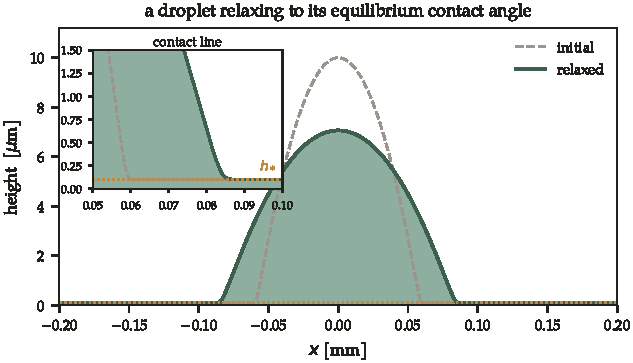
\includegraphics[width=0.85\textwidth]{../figures/wetting.pdf}
  \caption{A drop finding its equilibrium, from \file{wet\_static.toml} at
    $\thetae = \ang{10}$. The initial condition (dashed) is the equilibrium
    droplet of \ang{20}, \SI{10}{\micro\metre} high, on a precursor film of
    $\Hstar = 0.01$ (\SI{0.1}{\micro\metre}, dotted), resolved by
    $\Delta x = \SI{0.2}{\micro\metre}$; the solid curve is the free surface
    when the run has reached a steady state, at \SI{2.92}{\second}. The drop has
    spread to an apparent angle of \ang{9.71}, below $\thetae$ by the
    precursor bias of the next section, and the flat film around it settles
    \SI{0.5}{\percent} above $\Hstar$ ($\Hf$ of \cref{eq:Hf-Hmax}). The
    inset shows the contact line.\label{fig:wetting:relax}}
\end{figure}

\section{The apparent contact angle and the precursor bias}
\label{sec:wetting:apparent}

The equilibrium drop of a model with a \emph{finite} precursor does not show
the angle $\thetae$ unless $\Hmax/\Hstar$ is large. Outside the drop, where
disjoining pressure has died away, \cref{eq:eq-ode} reduces to $H'' = K$ and
the profile is a parabola. Extrapolating that parabola down to $H = 0$ and
reading its slope there is what corresponds to the angle measured
experimentally. It can be written in closed form:

\begin{equation}\label{eq:theta-cap}
  \thetacap = \varepsilon\,\sqrt{-2 K \Hmax}
            = \thetae \left( 1 - \frac{\Hstar}{2\Hmax} \right).
\end{equation}

\Cref{tab:apparent-angle} evaluates \cref{eq:theta-cap} for $\thetae = 10^\circ$
and $(n,m) = (3,2)$, alongside the largest slope the computed profile actually
attains anywhere.

\begin{yzntable}{Apparent angle and maximum profile slope, for $\thetae = 10^\circ$ and $(n,m)=(3,2)$\label{tab:apparent-angle}}{@{}d d d@{}}
\textsf{\bfseries $\Hmax/\Hstar$} & \textsf{\bfseries apparent angle [deg]} &
\textsf{\bfseries max.\ slope of the profile [deg]} \\ \midrule
2    & 7.5000 & 0.6320 \\
5    & 9.0000 & 3.6012 \\
10   & 9.5000 & 5.4236 \\
20   & 9.7500 & 6.7634 \\
50   & 9.9000 & 7.9627 \\
100  & 9.9500 & 8.5652 \\
1000 & 9.9950 & 9.5504 \\
\end{yzntable}

\begin{warn}[At $\Hmax/\Hstar = 2$ the model does not contain the angle you asked for]
  Read the first row. With a drop only twice as thick as its precursor, the
  apparent angle is $7.50^\circ$ and the steepest point of the profile is
  inclined at $0.63^\circ$. The $10^\circ$ that was written into
  \key{ContactAngle} is simply not present anywhere in the solution --- not as
  a measured value, not as a slope, not as an asymptote. This is not a
  discretization error and no mesh will remove it.

  Concretely: \textbf{a \SI{10}{\micro\metre} drop sitting on a
  \SI{2}{\micro\metre} precursor is not a valid case for measuring a contact
  angle.} If the number you want out of a run is an angle, size the case so
  that the ratio is large, using \cref{tab:apparent-angle} to decide how large.
\end{warn}

Note also how much more slowly the third column converges than the second. Even
at $\Hmax/\Hstar = 100$ the steepest slope in the profile is $8.57^\circ$,
short of $10^\circ$ by some 14 \%, while the apparent angle is already within
0.5 \%. \textbf{If you intend to measure the angle from the slope of the
computed profile rather than from the parabolic extrapolation, you need a
substantially thicker drop again.} \Cref{tab:apparent-angle} can be reproduced
with \code{tools/\bk make\_equilibrium\_1d.py --out /dev/null --sweep}. The
sweep writes no file, but \code{--out} is a required argument all the same, so
it needs a destination to throw away.

\section{Sizing a case}
\label{sec:wetting:sizing}

The length over which the profile changes from the precursor to the bulk drop
is

\begin{equation}\label{eq:transition-length}
  \ell = \frac{\hstar}{\thetae},
\end{equation}

with $\thetae$ in radians. For $\thetae = 10^\circ$ and
$\hstar = \SI{0.2}{\micro\metre}$ this gives $\ell = \SI{1.15}{\micro\metre}$.
Two requirements follow from it, and between them they fix the mesh.

\begin{tip}[Two rules of thumb for a contact-line case]
  \begin{itemize}
    \item \textbf{To resolve the contact line, aim for $\Delta x \le \ell/5$.}
      If the transition region is not resolved, neither the speed at which the
      contact line moves nor the angle it makes comes out right.
    \item \textbf{To obtain the angle you asked for, aim for
      $\Hmax/\Hstar \ge 50$} --- the drop height divided by the precursor
      thickness. By \cref{tab:apparent-angle} this keeps the error in the
      apparent angle within 1 \%. A ratio of 10 leaves you 5 \% out, and a
      ratio of 5 leaves you 10 \% out.
  \end{itemize}
  These are rules of thumb, not theorems. They are round numbers read off
  \cref{tab:apparent-angle} and off the width of the transition region; they
  tell you where to start, not where the answer is guaranteed to be converged.
  Confirm convergence by refining (\cref{ch:convergence}).
\end{tip}

A worked example. Take $h_0 = \SI{10}{\micro\metre}$ and
$\hstar = \SI{0.2}{\micro\metre}$, that is, a \key{PrecursorRatio} of
\val{0.02}, with $\thetae = 10^\circ$, on a domain \SI{600}{\micro\metre} wide
and \key{Grid.Nx} $=$ \val{2000}, giving $\Delta x = \SI{0.3}{\micro\metre}$. The
thickness ratio is exactly 50, so the second rule is met exactly. The first is
not: $\ell/5 = \SI{0.23}{\micro\metre}$, and $\Delta x = \SI{0.3}{\micro\metre}$
is $\ell/3.8$, slightly \emph{coarser} than the guideline. The case sits right
at the borderline rather than inside it --- which is how
\file{docs/validation.md} describes it. Measured there, the spread droplet
and the independently constructed equilibrium droplet agree to
\SI{0.02}{\percent} in apparent angle at this resolution, and so they do at
$\Delta x = \SI{1.2}{\micro\metre}$, where $\Delta x \approx \ell$; the spreading
itself follows the fine mesh's to \SI{0.06}{\percent}
(\cref{sec:verification:spreading}). That case is a lenient one, a single
\ang{10} droplet; the rule is a starting point, and refining is what tells.

The two rules pull against each other, and that is what makes contact-line
calculations expensive. Lowering $\hstar$ is the obvious way to buy a larger
$\Hmax/\Hstar$ --- but by \cref{eq:transition-length} it shortens $\ell$ in the
same proportion, so the mesh you need becomes finer by the same factor. You
cannot improve the angle for free; you pay for it in cells. That trade-off, not
the physics, is usually what sets the cost of a wetting run.

One last coupling to keep in mind. If the case also evaporates, $\hstar$ enters
the drying behavior as well, because the precursor correction $f_h$ of
\cref{sec:terms:evaporation} is what stops the precursor film drying out and
vanishing, and it is defined in terms of $\Hstar$. Changing the precursor
thickness to tune the contact angle changes the evaporation model at the same
time.

% ch-concentration.tex -- theory: the two concentration models, material properties, boundary conditions
\chapter{Concentration and boundary conditions}
\label{ch:concentration}

Two things remain to be explained about the model: how the solute is
transported, and what happens at the edges of the domain. They are grouped here
because both are choices you make in the input file that change the answer
rather than merely the cost, and because both are easy to make carelessly.

Yuzen offers two concentration models. \val{"WM"} is well mixed and treats the
concentration as uniform across the film thickness; \val{"CZ"} resolves the
distribution through the thickness. Both are available in one and two
dimensions. The first supports every physics term; the second gives up two of
them. Which one is right
depends on a single dimensionless number, and \cref{sec:conc:wm} says which.

\section{The well-mixed model}
\label{sec:conc:wm}

\key{Physics.ConcField.Model = "WM"} assumes the concentration is uniform
across the thickness. There is one unknown $c(x,y,t)$ per point and no mesh in
the thickness direction at all, which is what makes the model cheap. It solves
\cref{eq:conc-dim}.

The assumption is sound when diffusion across the thickness is much faster than
evaporation removes solvent from the surface, that is, when the P\'eclet number

\[
  \Pen = \frac{E_0 h_0}{D_0}
\]

is small. A thin film of a low-viscosity solvent that dries slowly is well
mixed to a very good approximation.

When $\Pen$ is not small the assumption fails, and it fails in a specific and
consequential way. Only the region near the free surface becomes concentrated,
and in reality that region forms a hard skin which then slows all subsequent
drying. The well-mixed model cannot represent this at all. Its errors follow
from one another:

\begin{itemize}
  \item there is no skin, because there is no cross-film structure to form one
    from, so drying does not slow down when it should;
  \item the surface concentration is \textbf{under-predicted}, since the
    solute that should have accumulated at the surface has been averaged over
    the whole thickness;
  \item the rise in viscosity is therefore weaker than it should be, because
    the exponential law of \cref{eq:prop-mu} is evaluated at too low a
    concentration;
  \item and the Marangoni stress is weaker too, because it is driven by the
    surface concentration gradient, which has been smoothed away.
\end{itemize}

Note that these are not independent errors that might partly cancel: they all
come from the same missing structure and all push in the same direction,
toward a film that stays more mobile for longer than the real one.

The equation is solved as the balance of the solute $hc$ of each cell: the
solute that crosses a face is the concentration there times the very volume
flux the film-height equation puts through that face in the same step, so the
solute of a closed film is kept to rounding, with evaporation or without, and
a uniform concentration stays uniform whatever the film does
(\cref{sec:disc:wm-conservative}). $c$ is kept within $[0, 1]$ by moving
solute between cells, never by cutting it (\cref{sec:disc:convection}).

\key{EnableConvection} and \key{EnableDiffusion} switch off the convective and in-plane
diffusive terms individually, which is useful for isolating one mechanism in a
test but is not a physical setting.

\section{The \texorpdfstring{\val{"CZ"}}{CZ} model: resolving the thickness direction}
\label{sec:conc:cz}

\key{Physics.ConcField.Model = "CZ"} solves for the concentration with the
thickness direction resolved: $c(x,z,t)$ with \key{Grid.Dimension = "xh"}, and
$c(x,y,z,t)$ with \key{Grid.Dimension = "xyh"}, which is the pseudo-3D case ---
the film spreads in $x$ and $y$ while the concentration is also resolved
across it. The film is mapped onto a fixed coordinate $\zeta \in [0,1]$, so
that as the film thins the $\zeta$ mesh contracts with it and the number of
cells through the thickness stays constant. That number is \key{Grid.Nz}.

Both dimensions are handled by the same code; the film's dimension is decided
by the grid, and with $N_y = 1$ no $y$ term is formed at all. The two-dimensional
case adds the mixed $x$--$y$ terms to the film-height equation and the
$y$--$\zeta$ cross terms to the concentration equation. \file{concz\_2d.toml}
is a worked example.

The boundary conditions in $\zeta$ are what make the model do its job. The
concentration equation is solved in conservative form for $hc$ on the $\zeta$
grid: each cell exchanges solute through face fluxes, and the flux through its
$\zeta$ faces follows from the discrete conservation of the grid with the
film's step, so a uniform concentration stays uniform and the solute of a
closed film is kept to rounding. No solute crosses the substrate or the free
surface: the total flux there, the advection by the evaporating solvent and
the whole diffusive flux, including its part along the slope of the surface
or the substrate, is zero. The solvent that leaves the top cell without its
solute is what builds up the concentrated layer near the surface. The rate of
evaporation itself is evaluated with \textbf{the free-surface concentration},
not the depth average, which is the whole point: it is what allows the surface
layer to slow its own drying, the effect the well-mixed model is missing.

\begin{figure}[tbp]
  \centering
  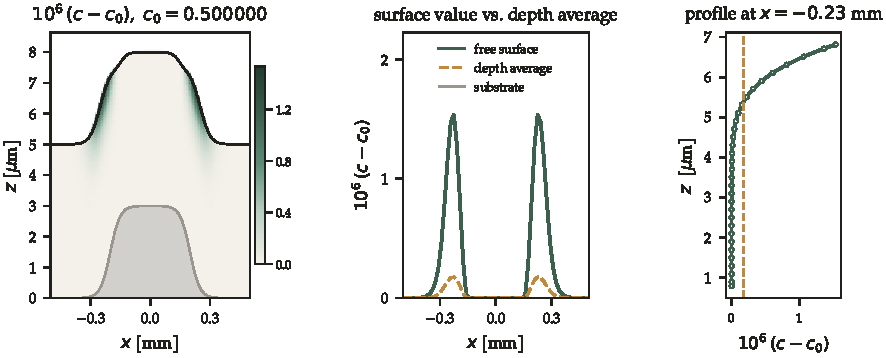
\includegraphics[width=\textwidth]{../figures/concz.pdf}
  \caption{What the \val{"CZ"} model resolves that the well-mixed one cannot,
    from \file{concz\_2d.toml} on the plane $y = 0$ at the end of the run.
    \textbf{Left:} the film over the substrate relief, colored by $c$ less
    the value $c_0$ it started at; the departure is in the seventh decimal.
    The solute sits in
    a layer hugging the free surface, and it is visible on the two shoulders
    and nowhere else. \textbf{Center:} the free-surface value, the depth average and the
    substrate value along $x$. They separate sharply at the two places where
    the film is thinnest, because the same evaporative flux is concentrated
    into less liquid there; everywhere else they are indistinguishable.
    \textbf{Right:} the profile through the thickness at that point, on the
    $\zeta$ grid the model uses, with the depth average marked. A well-mixed
    run carries only the dashed value, and it is the solid curve's top point
    that sets the surface tension and the evaporation rate.
    \key{Fluid.\bk Diffusivity} in that case is set below the value the 1-D
    cases use, on purpose: raise it back and diffusion halves the step.
    How far below is a measured choice
    rather than a free one, because the layer is about $\sqrt{D t}$ deep and
    the cells are \SI{0.2}{\micro\metre} high. At \num{3e-10} the layer spans
    four cells and the height of the step converges at second order in the
    cell height; two orders lower it is thinner than one cell and the step
    scales with the mesh instead. The case file carries the
    numbers.\label{fig:conc:czprofile}}
\end{figure}

Two further consequences follow from letting the viscosity vary through the
thickness. The in-plane velocity can no longer be written down analytically as
a parabola, so it is constructed by integrating $1/\mu$ and $z/\mu$ numerically
across the thickness. And the film thickness itself is then advanced with the depth integral of
that profile as its flux --- the kinematic condition at the free surface ---
rather than with a closed-form one; the surface tension in it is that of the
surface concentration.

The costs are real and you should weigh them before choosing this model. The
number of concentration unknowns grows from $N_x$ to $N_x \times N_z$. More
importantly, the set of physics terms available shrinks:

\begin{warn}[\val{"CZ"} has no disjoining pressure and no source term]
  The terms \val{"CZ"} supports are capillary pressure, solutal capillarity,
  vertical gravity, in-plane gravity, centrifugal force and evaporation.
  \key{Physics.DisjoiningPressure} and the whole of \key{Physics.Source} are
  \textbf{not available}, and are ignored without a diagnostic
  (\cref{sec:ref-physics:disjoining}). Since disjoining pressure is what
  produces a contact line, \textbf{every contact-line problem must use}
  \val{"WM"}. There is no way to combine a resolved cross-film concentration
  with a moving contact line in the present solver.
\end{warn}

\section{Concentration dependence of the material properties}
\label{sec:conc:properties}

The \key{Fluid} block gives each property at a reference concentration
\key{BaseConc} and the law by which it varies away from it
(\cref{sec:ref-domain:fluidconc}):

\begin{align}
  \sigma(c) &= \mathrm{BaseValue}
    + \mathrm{Coef}\,(c - \mathrm{BaseConc}),
    \label{eq:prop-sigma}\\
  \mu(c) &= \mathrm{BaseValue}\,
    \exp\bigl(\mathrm{Exponent}\,(c - \mathrm{BaseConc})\bigr),
    \label{eq:prop-mu}\\
  D(c) &= \mathrm{BaseValue}\,
    \exp\bigl(\mathrm{Exponent}\,(c - \mathrm{BaseConc})\bigr).
    \label{eq:prop-diff}
\end{align}

Surface tension is linear in concentration; viscosity and diffusivity are
exponential.

\Cref{eq:prop-mu} is the strongest non-linearity in the solver, and it is worth
being specific about how strong. \key{Fluid.Viscosity.Exponent} can reasonably
be around 10, and at that value \textbf{a change in concentration of 0.1
multiplies the viscosity by $e$}. Over the course of a drying run the
concentration may move by several tenths, so the viscosity can rise by orders
of magnitude. This is not a numerical inconvenience --- it is the physics of
the film solidifying and the flow stopping --- but it is also the reason the
Newton iteration and the time-step controller have to work hardest late in a
drying run (\cref{ch:convergence,ch:timeintegration}).

The coupling closes in both directions, and through more than one route.
\Cref{eq:prop-sigma} feeds two places at once: its slope \key{Coef} is the
Marangoni number $\Ma$ that drives \cref{eq:q-sc}, and $\sigma(c)$ also sits in
the mobility of the capillary-pressure term \cref{eq:q-cap}, so drying changes
how fast the film levels even with the Marangoni stress switched off. Viscosity
enters \emph{every} flux term through $\mu(c)$. So the concentration field
determines the flow, while the flow --- through convection in
\cref{eq:conc-dim}, and through the thickness that divides the evaporation term
of \cref{eq:conc-adv}
--- determines the concentration field. The two equations are coupled both
ways, which is why they are solved together rather than in sequence.

\section{What the boundary conditions mean physically}
\label{sec:conc:boundaries}

The height equation is fourth order, so \textbf{each boundary needs two
conditions, not one}. That is why you choose a named type rather than writing a
value: each name stands for a pair. The concentration equation is second order
and takes one condition from the same name. The types are set with
\key{Boundary.XminBC.Type} and its three siblings; the keys are listed in
\cref{ch:ref-bcout} and the way each pair is actually imposed on the mesh is in
\cref{ch:discretization}. What follows is what each one \emph{represents}.

\paragraph{\val{"Symmetry"}} A plane of symmetry. Nothing crosses it, and both
the shape and the concentration are mirrored through it. It has two quite
different uses: putting the center of a drop or a film on the boundary to halve
the cost of the calculation, and standing in for a closed wall. It is the
default.

\paragraph{\val{"Periodic"}} The edge is joined to the opposite one. Use it for
a film on a periodically structured substrate, or to compute a single
wavelength of a pattern that in reality continues indefinitely. It must be
specified at \emph{both} ends of a pair; specifying it on one side only, in
1-D or in 2-D, is refused before the run starts, and so is a \val{"Periodic"}
edge with the centrifugal term (\cref{sec:ref-bcout:boundary}).

\paragraph{\val{"Pinning"}} The edge of the liquid is held. The thickness at
the boundary is prescribed and flow across the boundary is stopped, while the
concentration takes a zero-gradient condition; \cref{ch:ref-bcout} records what
value the thickness is actually held at. It represents the physical
situation of a liquid edge arrested by a step, an edge bead or a line of
contamination. Its value is that it gives you a film whose edge does not move
\emph{without} the disjoining pressure and without a resolved contact line ---
that is, without any of the cost described in \cref{sec:wetting:sizing}.

\paragraph{\val{"FreshInlet"}} An inflow. The \emph{concentration} at the
boundary is held at the value that was there when the run started; the
thickness is not, and is recomputed at every assembly from the current interior
points. So the composition of what arrives is fixed and its thickness is free
to drift with the solution. It represents liquid of constant composition
arriving at the upstream end of a coating operation.
\Cref{sec:ref-bcout:boundary} gives the mechanism.

\paragraph{\val{"Outlet"}} Free outflow. The high-order derivatives are set to
zero so that liquid leaves without the boundary imposing a shape on it. Use it
where the domain was cut for reasons of cost and you genuinely have no
information about what lies beyond.

One further point applies whatever you choose: the \key{Substrate} shape is
mirrored at every wall, regardless of the type given for the film and the
concentration, and continued from the other end across a \val{"Periodic"} pair
(\cref{sec:ref-bcout:boundary}).

\begin{warn}[The boundary type changes the answer, not just the accuracy]
  These are not interchangeable closures that differ in the third decimal
  place. A spreading drop that reaches a \val{"Symmetry"} boundary is hitting a
  wall: the liquid piles up there, the thickness rises, and the subsequent
  evolution is that of a confined drop. The same drop reaching an
  \val{"Outlet"} boundary simply leaves the domain. These are two different
  physical problems with two different answers, and the input file does not
  distinguish between them for you. Decide what the edge of your domain
  physically \emph{is} before you choose a type.
\end{warn}


\part{Numerical method}
% ch-discretization.tex -- numerical method: the grid, the ghost layers and the matrix rows
\chapter{Discretization}
\label{ch:discretization}

This chapter describes the mesh Yuzen works on: where a quantity is allowed to
sit, how the boundary is padded, and how a point on the grid becomes a row of
the matrix. It is the vocabulary the rest of \cref{ch:timeintegration,%
ch:convergence,ch:linearsolver,ch:reproducibility} is written in, and it is the
first thing to read if you intend to add a physical term. The equations being
discretized are \cref{eq:height,eq:flux} of \cref{ch:governing}; the keys that
size the mesh are in \cref{sec:ref-domain:grid}.

\section{The staggered grid and the eight site types}
\label{sec:disc:stagger}

Yuzen uses a uniform rectangular grid. Given the grid lines
$x = x_{\min} + i_x\,\Delta x$, there are only two places along each axis at
which a quantity can be stored:

\begin{center}
\begin{tabular}{@{}l l@{}}
\code{0} & on the grid line, at $x = x_{\min} + i_x\,\Delta x$ \\
\code{1} & halfway between two grid lines, at $x = x_{\min} + i_x\,\Delta x + \Delta x/2$ \\
\end{tabular}
\end{center}

Three axes, two choices each: the list of possible positions is therefore
exactly three bits long and has exactly eight entries. Those three bits are the
type \code{Stagger<SX,SY,SZ>} (\file{yuzen/src/grid/Stagger.h}), and
\cref{tab:site-types} names them.

\begin{yzntable}{The eight site types and their three-bit encoding\label{tab:site-types}}{@{}l l L{0.46\textwidth}@{}}
\textsf{\bfseries Bits $(x,y,z)$} & \textsf{\bfseries Name} &
\textsf{\bfseries Position} \\ \midrule
0,0,0 & \code{Node}  & the grid point \\
1,0,0 & \code{Xedge} & the edge along $x$ \\
0,1,0 & \code{Yedge} & the edge along $y$ \\
0,0,1 & \code{Zedge} & the edge along $z$ \\
0,1,1 & \code{Xface} & the face with normal $x$ \\
1,0,1 & \code{Yface} & the face with normal $y$ \\
1,1,0 & \code{Zface} & the face with normal $z$ \\
1,1,1 & \code{Cell}  & the cell center \\
\end{yzntable}

The reason for encoding the positions this way rather than tabulating them is a
single observation: \textbf{moving half a cell along an axis flips that axis's
bit, and nothing else changes}. Every change of site type in the whole code is
that one operation, and the accompanying movement of the index follows from the
same bit in one line --- moving $+\tfrac12$ cell raises the index by one when
the bit was already \code{1}, and moving $-\tfrac12$ cell lowers it by one when
the bit was \code{0}. There is no hand-written table of offsets to keep in step
with anything.

In 1-D only the $x$ bit carries meaning, and in 2-D the $x$ and $y$ bits do.
The unknowns sit on \code{Xedge} in 1-D, on \code{Zface} in 2-D, and the
concentration of the \val{"CZ"} model (\cref{sec:conc:cz}) sits on \code{Cell}
--- in each case half a cell along every in-plane axis, which is what
\cref{ch:governing} calls the cell center.

A field is declared as \code{Field<GRID,S,T>}, with the site type \code{S} as a
template parameter rather than as runtime data. A stagger mismatch is therefore
a compile error, not a wrong answer: you cannot pass a cell-centered field where
an edge-centered one is expected. The overloads of
\code{C\_FiniteDifferences::GradX} and its relatives, one per site type, exist
for the same reason --- the derivative of a field knows which way it has moved
by half a cell, because the type says so.

\section{Ghost layers}
\label{sec:disc:ghost}

Outside the boundary the grid carries \textbf{two ghost layers on each side}
(\code{C\_Grid*::NumGhostX()}). Two, not one, because the thickness equation is
fourth order: evaluating it at a boundary point reaches two neighbors away.

\key{Grid.Nx} counts interior points only, so a grid declared with
\key{Nx = 300} holds $\mathrm{Nx} + 4 = 304$ points along $x$. Remember this
when you estimate memory or read a row count out of a debug print.

\code{CheckGhost(s)} sorts every point into one of three classes:

\begin{description}
  \item[\code{Inside}] within the computational domain. This is the only place
    a physical term adds a contribution.
  \item[\code{bXmin}, \code{bXmax}, \dots] the boundary itself, where the
    boundary condition fixes the value. In 2-D the corners join this set, and
    in 3-D the edges as well.
  \item[\code{Outside}] the outermost ghost layer.
\end{description}

\section{From a point to a matrix row}
\label{sec:disc:rows}

The number of rows is the \textbf{total number of points including the ghosts},
$\mathrm{imax()} - \mathrm{imin()} + 1$ --- not the number of interior points.
The map from a point to its row number is collected in one place per dimension,
\code{Index()} in \file{GridTraits.h}, and is given in \cref{tab:row-index}.

\begin{yzntable}{The point-to-row map, one per dimension\label{tab:row-index}}{@{}l l@{}}
\textsf{\bfseries Dimension} & \textsf{\bfseries Row} \\ \midrule
1-D & $\mathrm{row} = i_x$ \\
2-D & $\mathrm{row} = n_x\,i_y + i_x$ \\
3-D & $\mathrm{row} = n_x n_y\,i_z + n_x\,i_y + i_x$ \\
\end{yzntable}

Ghost rows are marked as boundary-condition rows with
\code{CRS\_Matrix::SetAsBC()}. A marked row is excluded from the time
integration --- \code{MakeMatrix\_IA()} and \code{MakeRHS()} skip it --- and the
physical terms consult \code{IsBC()} and do not add to it either. The
coefficients of a boundary-condition row are written once at initialization and
survive every subsequent zeroing of the matrix, so they never have to be
rebuilt.

The stencil is five points in 1-D, written \code{M m o p P}: the point itself
and two neighbors on each side. In 2-D it is thirteen points --- the
nine-point cross, plus the four diagonals \code{mm}, \code{pm}, \code{mp},
\code{pp}. \textbf{The diagonals are not optional.} They are there because the
biharmonic operator contains the cross term
$\partial^4/\partial x^2\partial y^2$, whose difference coefficient is of order
$1/(\Delta x^{2}\Delta y^{2})$ and whose stencil is precisely the four
diagonal neighbors. Drop them and you are no longer discretizing
$\nabla^{2}\nabla^{2}$.

The order in which the columns of a row are inserted is fixed by the ordering
of \code{T::FullIdx(k)} and its relatives. That ordering is not cosmetic: it
sets the order of the floating-point additions in the matrix--vector product,
and changing it breaks bit-level reproducibility. See \cref{ch:reproducibility}.

\section{The mobility at a face, and why its form is not free}
\label{sec:disc:positivity}

The film-height equation is a fourth-order \emph{degenerate} diffusion: the
mobility $D(h) = h^{3}$ vanishes where the film does. That degeneracy is what
makes a contact line possible at all, and it is also what makes a careless
discretization produce negative film thickness. A face between two cells needs
a single mobility built from the two thicknesses on either side, and the choice
of how to build it decides whether the scheme can go negative.

The well-mixed model uses the positivity preserving interpolation of Diez and
Kondic (2002), their Eq.~(23):
%
\begin{equation}
  D_{k}^{(x)} \;=\; \frac{2\,h_{k}^{2}\,h_{k+1}^{2}}{h_{k} + h_{k+1}},
  \qquad
  D_{k}^{(y)} \;=\; \frac{2\,h_{k}^{2}\,h_{k+n_x}^{2}}{h_{k} + h_{k+n_x}} .
  \label{eq:disc:pps}
\end{equation}
%
This is not an ad-hoc average. It is the general prescription
%
\begin{equation}
  D_{i} \;=\; \frac{h_{i+1} - h_{i}}{g_{i+1} - g_{i}},
  \qquad
  g(h) \;=\; \int \frac{\mathrm{d}h}{D(h)} ,
  \label{eq:disc:pps-general}
\end{equation}
%
evaluated for $D(h) = h^{s}$ at $s = 3$. The implementation is
\code{NonlinearTerm()} in \file{model/well\_mixed/LaplacePressureKernel.h}.

Why this form and not another: \cref{eq:disc:pps} factorizes as the product
$h_k h_{k+1}$ with the harmonic mean $2h_k h_{k+1}/(h_k + h_{k+1})$, so when one
side thins it vanishes as $O(h^{2})$, and it is exactly zero when one side is.
The face flux therefore switches itself off at the edge of a dry region. The
obvious alternative, the arithmetic mean $(h_k^{3} + h_{k+1}^{3})/2$, retains a
mobility of $h_k^{3}/2$ against a completely dry neighbor, draws liquid out of
the dry region, and drives $h$ negative.

\begin{warn}[Do not simplify this expression]
Rewriting \cref{eq:disc:pps} as an arithmetic mean --- or as anything else that
does not vanish with the thinner side --- removes the positivity guarantee. The
symptom is not a crash but negative film thickness near a contact line, which
then poisons the viscosity and the concentration equation downstream. The
property is pinned by
\file{yuzen/tests/test\_positivity\_mobility.cpp}, which checks
\cref{eq:disc:pps} against \cref{eq:disc:pps-general}, checks that the mobility
falls as $O(h^{2})$ and reaches zero, and checks that the arithmetic mean fails
both.
\end{warn}

\subsection{One face mobility for the terms of the potential}
\label{sec:disc:positivity-one}

The disjoining pressure and the vertical gravity take the same face mobility,
\cref{eq:disc:pps} to the bit (\code{Mobility::Face}; zero when either side is
dry or is the ghost $-h$ of a \val{"Pinning"} edge). The flux of a face is
then one mobility times the difference of the whole potential
$\varphi = \hat\sigma\nabla^2(H+S) + \Dpn\,\Pihat(H) - \Bo\,(H+S)$
(\cref{sec:output:potential}), so the dissipation of the scheme,
$\sum_f D_f(\Delta\varphi)^2/\Delta x$, is a sum of squares: the discrete free
energy never rises (\cref{sec:output:energy}), and a steady film is one with
$\varphi$ uniform, the minimum of the discrete energy. The vertical gravity's
term over a relief, $D_f\,\Delta s$, enters $A$ as $K(h_a + h_b)\,\Delta s$
with $K = D_f/(h_a + h_b)$, the same share for the two cells of the face. The
two terms took the arithmetic mean $(h_a^3 + h_b^3)/2$ until \file{Energy.dat}
showed the free energy rising near a steady film; that mean also left a
disjoining-pressure flux of $h^3/2$ against a dry neighbor.

\subsection{The face mobility with Navier slip}
\label{sec:disc:positivity-slip}

With \key{Physics.Slip} (\cref{sec:ref-physics:slip}) the mobility is
$D(h) = h^{3} + a h^{2}$, $a = 3\Lambda$, and \cref{eq:disc:pps-general}
applies with
%
\begin{equation}
  g(h) = -\frac{1}{a h} + \frac{1}{a^{2}}\ln\frac{h+a}{h}
       = -\frac{x - \ln(1+x)}{a^{2}}, \qquad x = \frac{a}{h} .
  \label{eq:disc:pps-slip}
\end{equation}
%
Both forms cancel somewhere, and \file{model/Mobility.h} switches to a series
there: $x - \ln(1+x)$ is summed as $\sum_{n=2}^{18}(-1)^n x^n/n$ below
$x = 0.1$ (remainder below $5\times10^{-19}$ relative), and where the two
heights differ by less than $10^{-3}$ of their mean $\bar h$ the face mobility
is $D(\bar h)/(1 + \delta^{2}K/24)$, $\delta = h_{k+1} - h_k$,
$K = D\,(1/D)''$, with a truncation error $O((\delta/\bar h)^4) < 10^{-12}$.
Against a reference free of cancellation the largest relative error is
$4\times10^{-13}$, and the value is continuous to $10^{-12}$ across each switch.
Without slip none of this is reached: \cref{eq:disc:pps} is
evaluated as written. The disjoining pressure and the vertical gravity take
the same face mobility with slip as without (\cref{sec:disc:positivity-one}).

The face mobility still vanishes on a dry side, but near it
$D \sim a h^{2}$, so it vanishes as $O(h)$ rather than $O(h^{2})$.

\begin{warn}[Slip weakens the positivity guarantee]
With slip the degeneracy that keeps the film positive is one order weaker.
Where the film is held up by a disjoining pressure, or does not thin below a
fraction of its height (about $0.1\,h_0$), this has no visible effect; a film
driven toward zero thickness with no disjoining pressure can go negative where
it would not without slip. Watch \code{HHmin} in \file{History.dat}.
\end{warn}

\subsection{The same mobility in the \texorpdfstring{\val{"CZ"}}{CZ} model}
\label{sec:disc:positivity-concz}

The \val{"CZ"} model resolves concentration, and hence viscosity, through the
thickness, so its in-plane velocity is not analytic: \code{CalVelocity()} in
\file{model/ConcZ/CZ2D/CZ\_HeightEquation\_2D.cpp} integrates $1/\mu$ and
$z/\mu$ across the film by Simpson's rule, and the concentration equation
advects with the result.

The film height itself, however, is advanced in the same conservative form as
the well-mixed model,
%
\begin{equation}
  \frac{\partial h}{\partial t} = -\frac{\partial Q}{\partial x} - E ,
  \label{eq:disc:cz-conservative}
\end{equation}
%
with the flux at a face carrying the same mobility \cref{eq:disc:pps}, divided
by three because the depth-integrated flux is $h^{3}/3\mu$ rather than $h^{3}$.
Integrating the \val{"CZ"} velocity profile through the thickness reproduces that
factor exactly in the uniform-viscosity limit. The implementation is
\code{FaceMobility()}, and the well-mixed counterpart of the same $1/3$ is the
\code{\_Magnitude} of its capillary term.

\begin{note}[The resolved viscosity at the face]
The flux through a face is the depth integral of the resolved velocity
profile,
$Q = h^3 b\int_0^1 (1-\zeta)^2/\mu\,d\zeta + h^2\tau\int_0^1 (1-\zeta)/\mu\,d\zeta$,
with $b$ the driving pressure gradient and body force and $\tau$ the
Marangoni stress. The mobility therefore carries the mean of $1/\mu(c(\zeta))$
weighted by $3(1-\zeta)^2$, the Marangoni flux the mean weighted by
$2(1-\zeta)$, and the surface tension is that of the surface concentration
(\code{FaceInvViscosity()}, \code{FaceSurfConc()}). The positivity-preserving
$h$ factors are unchanged, and a uniform viscosity gives $h^3/3\mu$ exactly.
A mobility that takes one viscosity and one surface tension per face at the
depth-mean concentration would move the film with a flux that is not the
integral of the profile which carries its solute, and with a stratified
concentration its error does not fall with refinement
(\cref{sec:verification:mms}).
\end{note}

Because both models are conservative and share the mobility, they agree in the
limit where the concentration is uniform through the thickness --- and that
agreement is a genuine check, since the two reach it by different routes. The
comparison is run by \file{tools/concz\_vs\_wm.py} and is part of the test
suite as \code{concz\_vs\_wm}: setting \key{Fluid.Viscosity.Exponent} to \val{0}
and switching off evaporation and solutocapillarity leaves the concentration
unable to affect $h$, and the peak film thickness of the two models then agrees
to within $10^{-6}$ relative, with the volume of each conserved exactly and
the same in the two \file{History.dat}.

\begin{note}[Two traps when running this comparison]
Leave the adaptive time step on and the two models choose different step
histories, so their output times drift apart; comparing the last row of each
\file{History.dat} then compares two different instants, which produces a
difference of a few percent that moves around non-monotonically under
refinement and looks exactly like a discretization error. Fix the step. Second,
the output interval must be well below \key{EndTime}, or the only shared
instant is the initial condition and the models appear to agree perfectly.
\end{note}

\section{The convection schemes}
\label{sec:disc:convection}

Three kinds of term are convective: the advection of the concentration, and
in the well-mixed film-height equation the in-plane body forces and the
Marangoni flux, which enter as a film height carried by a velocity rather than
as the gradient of a mobility. Each needs the value of a field at a face, and
takes it from the four cells $f_{LL}, f_L, f_R, f_{RR}$ about the face. For
the fixed schemes this value is
%
\begin{equation}
  f_{\text{face}} = \sum_j c_{1,j} f_j + \operatorname{sign}(u)\sum_j c_{2,j} f_j ,
  \label{eq:disc:face}
\end{equation}
%
with $c_1 = (-1, 7, 7, -1)/12$ and $c_2 = (-1, 3, -3, 1)/12$ for UTOPIA, and
$c_2$ three times larger for Kawamura--Kuwahara. Both are third order; the
leading error of the advection they give is $-|u|\Delta x^3/12\,\partial^4 f$
and $-|u|\Delta x^3/4\,\partial^4 f$. \val{"Central4"} has no $c_2$: its face
value is fourth order, the divergence only second, with no dissipation.
UTOPIA is the uniformly third-order polynomial interpolation of Leonard,
MacVean and Lock (1993), the Kawamura--Kuwahara scheme that of Kawamura,
Takami and Kuwahara (1986) written as a face value, and \val{"QUICK"} the
quadratic upstream interpolation of Leonard (1979); all are listed in Further
reading.

At the face of a \val{"Symmetry"} or \val{"Pinning"} edge the three
upwinded terms of the film-height equation carry no flux: their mobility there
is set to zero in $A$, in the Jacobian and in the velocity
(\code{UpwindKernelBase::WallFace}). Their flux is not a gradient, and a
mirrored ghost does not make the face value zero.

The limited schemes write the face value from the upwind side. With
$(UU, U, D)$ the cells $(LL, L, R)$ for a flow in $+x$ and $(RR, R, L)$ for one
in $-x$, and the two differences $a = f_U - f_{UU}$, $b = f_D - f_U$,
%
\begin{equation}
  f_{\text{face}} = f_U + \tfrac12\,\Phi(a, b), \qquad
  \Phi_{\text{Koren}} = \operatorname{sign}(b)\min\!\left(2|a|,\ \tfrac{2|b| + |a|}{3},\ 2|b|\right), \qquad
  \Phi_{\text{vL}} = \frac{2ab}{a + b},
  \label{eq:disc:limited}
\end{equation}
%
and $\Phi = 0$ unless $a$ and $b$ have the same sign: the limiters of Koren
(1993) and van Leer (1974). Nothing is divided by a gradient that may vanish. Koren's is UTOPIA wherever $0.4 \le a/b \le 4$ and
bounded elsewhere: the face value never leaves the interval between $f_U$ and
$f_D$, and at an extremum it falls back to $f_U$. That is the price of the
bound: a smooth extremum is clipped to first order locally, which costs the
accuracy of a smooth solution, and the maximum error converges at about 1.5
rather than 3 on a sine. The mirror image of a stencil gives the same value
to the last bit, so the checks of \cref{sec:verification:equivalence} hold for
every scheme.

In the concentration equation, which is linear in $c$ once its coefficients
are fixed, a limited face value is frozen at the latest iterate: in the row of
the face's upwind cell it is written $f_U + \chi/2\,(f_U - f_{UU})$ with
$\chi = \Phi/a$, elsewhere $f_U + \psi/2\,(f_D - f_U)$ with $\psi = \Phi/b$. The
frozen matrix is then an M-matrix, and the explicit half of Crank--Nicolson is
positive for a Courant number up to one, so the step keeps $c$ within its
bounds there. The step is not held to that; a step past it is reported in
\file{Warnings.txt}, for this equation and for the film height alike
(\cref{sec:ref-numerics:convection}). The well-mixed concentration is re-solved on every Newton pass,
so the frozen values converge with the film; the step is completed with the
limiter frozen at its own answer (\cref{sec:disc:wm-conservative}), and the
explicit half of each step is formed from the state the step starts from,
with the limiter at that state. In \val{"CZ"} each
stage uses the concentration it is evaluated at, which is the midpoint rule of
the limited operator.

\paragraph{$0 \le c \le 1$ without cutting or making solute.} The
concentration is a mass fraction, and each completed step is brought into
$0 \le c \le 1$. With the evaporation limited to the solvent there is
(\cref{sec:terms:evaporation}) only rounding passes 1 --- and the over- and
undershoot of an unbounded scheme at a sharp front: KK, UTOPIA, Central4 and
QUICK at any Courant number, Koren and van Leer above one. In the well-mixed
model what a real cell holds above 1, $h(c-1)$, goes to its face neighbors in
proportion to the room they have, $h(1-c)$; what they cannot take goes on in
a further pass from the cells it then sits in, up to four, and what is left
after them is spread over every cell with room, in proportion to it. A cell
below 0 is filled the same way the other way round: what it lacks, $-hc$, is
taken from its face neighbors in proportion to the solute $hc$ they hold, in
up to four passes, and then from every cell holding solute. The cells have
equal area, so the sum of $hc$ that \code{ResinVolErr} balances
(\cref{sec:output:history}) is kept to rounding, and the ghosts are formed
again from the cells as moved. Each pass takes the room of every cell before
it moves anything, so the result does not depend on the order of the cells,
and where no cell leaves $[0, 1]$ nothing is touched. Only a film holding more
solute than liquid in all, or less than none, would leave a remainder; it
would be cut, or made up, and reported in \file{Warnings.txt}.
\file{JobInfo.txt} gives the solute moved over the run
(\cref{sec:output:jobinfo}). Left below 0, the undershoot of a front from
$c = 0.7$ to $0.005$ reached $-0.04$ to $-0.09$ and, past the divergence test
of $-0.1$, stopped the run with QUICK and Central4, and with UTOPIA at
Courant 1.5 (found; corrected). Within the Newton passes the working field from
which the viscosity, the Marangoni stress and the evaporation are taken is
capped at 1, but the limiter of Koren and van Leer is frozen at the iterate as
the equation solved it: frozen at the capped values, the two rows that share a
face would take different face values from it, and the advection would lose
its flux form there. In \val{"CZ"} the excess of a cell goes to the cell
below it in its column, whose cells have the same volume; a column whose mean
passes 1, which the solvent limit prevents, keeps $c$ above 1 with a warning.
A cell below 0 is filled from the cells of its column that hold solute, in
proportion to it; a column whose mean is below 0, which is what the
undershoot of the advection along the film makes, takes what it lacks from
the columns next to it in proportion to their solute (each scaled as a whole,
so no cell of theirs goes below 0), in up to four passes and then from every
column holding solute, as the well-mixed cells do
(\code{CZ\_HeightEquation\_2D::RedistributeDeficit}). Left below 0, a front
of \val{"CZ"} from 0.7 to 0.005 with UTOPIA at Courant 0.4 passed the
divergence test and stopped the run (found; corrected).

In the film-height equation the matrix $A$ holds the face weights frozen at
the current film, so that $A(h)h$ is the flux exactly, and the Jacobian adds
the rest of the derivative of the limited face height $h_f$: with
$g = \partial h_f/\partial h$, $w(3g - w_t)h_f^2/\mu$ for the body forces and
$(2g - w_t)h_f\,\Delta c/\mu$ for the Marangoni flux. Newton keeps its
quadratic convergence (\cref{sec:verification:schemes}); at the kinks of
Koren's $\Phi$ the derivative is one-sided. The Marangoni flux is upwinded by
the direction of the flux itself, the sign of $\sigma_c\,\Delta c$, not of
$\Delta c$ alone, which would pick the downwind side with a negative
\key{Fluid.SurfaceTension.Coef}.

\subsection{The well-mixed concentration in conservative form}
\label{sec:disc:wm-conservative}

The well-mixed concentration equation is solved as the finite-volume balance
of the solute $hc$ of each cell over the step,
%
\begin{equation}\label{eq:disc:wm-conservative}
  \begin{aligned}
    h^{1}c^{1} - h^{0}c^{0}
      = {}& -\Delta t \sum_f s_f \bigl[\theta\,G_f^{1} + (1-\theta)\,G_f^{0}\bigr]
        + \Delta t\,S\,c_S \\
      &{} - \Delta t\,\bigl[\theta\,r^{1}c^{1} + (1-\theta)\,r^{0}c^{0}\bigr],
    \qquad
    G_f = F_f\,c_f - D(c_f)\,h_f\,\frac{c_{\mathrm{hi}} - c_{\mathrm{lo}}}{\Delta x},
  \end{aligned}
\end{equation}
%
$s_f = \pm 1/\Delta x$ the outward sign of face $f$ over the spacing across
it, $\theta = 1/2$. $F_f$ is the volume flux the film-height equation puts
through that face: the sum, over the enabled terms, of what each holds in $A$
for it --- the capillary, vertical-gravity and disjoining fluxes, and the
in-plane body forces, the centrifugal force and the Marangoni stress with
their upwinded face heights (\code{FaceFlux} of each kernel). $c_f$ is the
face value of \key{Numerics.Convection.Concentration} (\cref{eq:disc:face}),
upwinded by the sign of $F_f$; $D(c_f)\,h_f$ takes the means of the two cells.
$S$ is the liquid the nozzle supplies, at the middle of the step as the
film-height equation takes it, and $c_S$ the concentration it arrives at:
$c_S = \theta c^{1} + (1-\theta)c^{0}$, the concentration it lands on, with
\key{Physics.Source.ConcType = "local"} (the default), and
$c_S = \key{Physics.Source.Conc}$ with \val{"supplied"}, which mixes the new
liquid through the thickness of the cell's column: on a film with no flow,
$c^{1} = (h^{0}c^{0} + \Delta t\,S\,c_S)/(h^{0} + \Delta t\,S)$.
$r$ is the sideways outflow of the 1-D centrifugal term, which
leaves at the concentration of its cell. Evaporation takes solvent only and
does not appear: it is in $h^{1}$. This is \cref{eq:conc-dim} itself; the form
of \cref{eq:conc-adv} for $c$ agrees with it in the continuum, but discretely
only the balance keeps the solute. Solved for $c$ in the form of
\cref{eq:conc-adv}, a front from 0.9 to 0.3 on a closed
periodic film, carried by the flow and drying by Raoult's law, lost
$1\times10^{-5}$ to $3\times10^{-4}$ of its solute, depending on the scheme
and the grid (50 to 200 cells), over 0.3 of a crossing of the domain (found;
corrected: now $4\times10^{-16}$ to $3\times10^{-15}$ in 1-D and
$2\times10^{-14}$ in 2-D, \code{conc\_drying} in
\cref{sec:verification:analytic}).

The equation is solved for the change $d = c^{1} - c^{0}$ of the step. Taking
$c^{0}$ times the film's own step,
$h^{1} - h^{0} = -\Delta t \sum_f s_f[\theta F_f^{1} + (1-\theta)F_f^{0}]
- \Delta t\,[\theta r^{1} + (1-\theta)r^{0}] - \Delta t\,(E - S)$, from
\cref{eq:disc:wm-conservative} leaves
%
\begin{equation}\label{eq:disc:wm-change}
  \begin{aligned}
    &h^{1} d + \theta\Delta t \sum_f s_f\bigl[F_f^{1} d_f - K_f^{1}(d_{\mathrm{hi}} - d_{\mathrm{lo}})\bigr]
       + \theta\Delta t\,(r^{1} - S)\,d \\
    &\quad= -\Delta t \sum_f s_f \bigl[\theta F_f^{1} + (1-\theta)F_f^{0}\bigr](c^{0}_f - c^{0})
       + \Delta t\,E\,c^{0} \\
    &\qquad\quad{}+ \Delta t \sum_f s_f \bigl[\theta K_f^{1} + (1-\theta)K_f^{0}\bigr](c^{0}_{\mathrm{hi}} - c^{0}_{\mathrm{lo}}),
  \end{aligned}
\end{equation}
%
$K_f = D(c_f)h_f/\Delta x$, every face value $c^{0}_f - c^{0}$ formed as the
sum of the face weights times $c^{0}_k - c^{0}$. The weights sum to one, so a
uniform $c^{0}$ gives a right-hand side of exactly zero without evaporation,
and $d = 0$; the evaporation, $\Delta t\,E\,c^{0}$, concentrates the solute
as $h^{1}c^{1} = h^{0}c^{0}$ where nothing else acts. With
\key{EnableConvection} off the terms in $c_f - c$ are dropped, and the film
still thins or thickens under the solute ($\theta\Delta t \sum_f s_f
F_f^{1} d$); the solute is then not a balance, since the flow moves liquid
without the solute in it, and the step ends with $c^{0} + d$.

The film $h^{1}$ comes from the Newton iteration of the same step. On every
pass the concentration is solved with the film of that pass and its fluxes
(\cref{sec:time:coupling}); these give that film only once the iteration has
converged. The step is then completed (\code{AfterNKLoop} of
\file{HeightEquationBase.h}). The film is the one the iteration converged
to; the fluxes, the sideways outflow and the supply are taken at it, with the
concentration of the last pass, and the evaporation as that pass took it.
What their divergence still misses of the step the film took, cell by cell,
is the residual of the step at that film; less its mean over the cells, which
is the volume error of the step and stays as that, it is added to the fluxes
of the inner faces as running sums --- along $y$ the sum of each row of cells
spread evenly over the row, then along $x$ within each row what is left of
it --- so that the face fluxes are exactly those of the step the film took
(\code{ConsistentFluxes}). No edge face and no wall is touched, and nothing
is solved. The film the fluxes would give instead, $h^{0}$ less their
divergence, differs from the converged one by that residual, and on a film far
thicker than its cells the residual is at the rounding of fluxes of enormous
size ($\epsmach\,\Delta t/\Delta t_{\mathrm{explicit}}$,
\cref{sec:convergence:floor}): taken as the film, it goes negative in
\file{nozzle\_1d\_rotating}. The concentration is then
solved once more with these fluxes and this film, and the solute of each cell
is formed from \cref{eq:disc:wm-conservative} with the solute flux of each
face formed once, from the four cells about it whichever side asks
(\code{Reconstruct} of \file{ConcEquationBase.h}): the sum of $hc$ over the
cells changes by the fluxes through the edges and the sources alone, to
rounding, whatever the tolerance of the linear solve. Those edge fluxes, the
volume flux of each edge face (which \code{ConsistentFluxes} leaves alone)
and the solute flux \code{Reconstruct} formed there, are what
\file{History.dat} counts as crossing a \val{"FreshInlet"} or an
\val{"Outlet"} (\cref{sec:output:history}). A limited scheme is
solved again with its limiter frozen at its own answer until that settles
($10^{-12}$, at most eight times), so that the face values of the step are
the limited face values of the answer. Then $c$ is brought into $[0, 1]$
(\cref{sec:disc:convection}). A pass, or the end of a step, whose film has a
cell without liquid ($h \le 0$, at a step far too long for the film) leaves
the concentration as the pass before had it: the balance of $hc$ is not one
there, and the step is left to fail on the film (found: the
solve failed first and the run stopped naming the concentration solver;
corrected). At such a step the Newton correction of the film stagnates far
from convergence, and the step is cut, or at a fixed step the run stops
naming the stagnation (\code{wm\_diverges} in \file{tools/input\_guards.py},
\cref{sec:convergence:stagnation}); a film that is below zero all the same,
as one read from a file, stops the run as diverged (\code{wm\_film\_below}).

A uniform concentration under a strong in-plane flow, a nozzle, the vertical
gravity, the capillary pressure and, in 1-D, the spin stays uniform to
$6\times10^{-16}$ (\code{conc\_uniform}) --- in general to the rounding of
the solute fluxes relative to the film, $\epsmach\,\Delta t\sum_f|F_f|/h$,
which the solute formed from them once more carries (up to $3\times10^{-12}$
in \file{tools/proptest.py}, on a thin film next to a \val{"Pinning"} edge); with every term of the model the
manufactured solutions converge at second order in $\Delta x$ and $\Delta t$
(\cref{sec:verification:mms}), and the oblique wave of
\cref{sec:verification:schemes} at 1.91 and 1.97.

\subsection{The concentration of \texorpdfstring{\val{"CZ"}}{CZ} in conservative form}
\label{sec:disc:cz-conservative}

The \val{"CZ"} concentration equation is a finite-volume balance of $hc$ on
the $\zeta$ grid. The film-height equation stores the flux through each of
its faces and writes the end of the step as their divergence; the
concentration equation splits each of these into layer fluxes, the cell mean
of the resolved velocity profile adjusted so that the layers of a column add
up to the film-height flux face by face. The flux through the $\zeta$ faces
then follows from the discrete conservation of the grid, built up from the
substrate, with the evaporating solvent leaving through the surface face.
The ghost cells above the surface and below the substrate are set so that
the total flux there --- advection and the whole diffusive flux, its part
along the slope included --- is zero. The step is solved for the change of
$c$, so a uniform $c$ gives exactly no change, and the small solute residual
of the linear solver is put back as a uniform shift of the change, sized for
the solvent the shift itself sends through the surface term and applied to
the ghosts as well (each side of a periodic seam forms the flux there from
its own), so that the solute of the step balances to rounding. The limited schemes keep
their frozen upwind and downwind forms, which keep $c$ bounded, and are
re-solved until the limiter has settled at the midpoint of the step.

The scheme of \key{Numerics.Convection.Concentration} is used on every face,
$x$, $y$ and $\zeta$ alike. With the central schemes nothing is dissipated in
any direction, so the solution has what the model has at the shortest waves
the grid resolves: a film stratified with $\sigma_c\,\partial c/\partial\zeta
> 0$ and a weak diffusivity is unstable there, and a central scheme lets
those waves grow where an upwind-biased one damps them on a coarse enough
grid (\cref{sec:verification:schemes}).

% ch-timeintegration.tex -- numerical method: theta method, Newton, coupling and the adaptive step
\chapter{Time integration}
\label{ch:timeintegration}

Every equation Yuzen solves is cast into the same shape, advanced with the same
$\theta$ method, and --- where it is non-linear --- driven to the solution of
the implicit system by the same outer Newton iteration. This chapter describes
that machinery: the form, the iteration, the Jacobian, the way the thickness
and the concentration are coupled, and the adaptive time step. The keys
mentioned here are documented in \cref{sec:ref-numerics:height,%
sec:ref-numerics:tsc}; what happens when the iteration will not converge is the
subject of \cref{ch:convergence}.

\section{The form every equation is cast into}
\label{sec:time:form}

Every equation is rearranged into

\[
  \frac{\partial\varphi}{\partial t} = -A\,\varphi - B
\]

before it is handed to the solver (\file{numerics/ImplicitSolver.h}). $A$ is
the part proportional to the unknown, and is a matrix; $B$ is everything else,
and is a vector. Time is advanced with the $\theta$ method, where
$\theta = 0$, $0.5$ and $1$ are forward Euler, Crank--Nicolson and backward
Euler respectively. \textbf{Both the thickness equation and the concentration
equation are built with Crank--Nicolson}, $\theta = 0.5$.

The system actually solved for the correction $\delta\varphi$ is

\begin{equation}\label{eq:nk-update}
  (I + \theta\,\Delta t\,J)\,\delta\varphi
    = \varphi_{\mathrm{old}} - \varphi_{\mathrm{guess}}
      - \Delta t\left[\theta\,A\cdot\varphi_{\mathrm{guess}}
        + (1-\theta)\,A\cdot\varphi_{\mathrm{old}} + B\right],
\end{equation}

with $J$ the Jacobian of \cref{sec:time:jacobian}. The right-hand side of
\cref{eq:nk-update} is the residual, and it is worth noting now that it is
also the origin of the correction floor of \cref{sec:convergence:floor}.

\begin{warn}[A term in $B$ has to be averaged in time as well]
  The $\theta$ weighting of \cref{eq:nk-update} applies to $A$. A term put into
  $B$ gets it only if $B$ itself is formed as the same average, and the
  well-mixed thickness equation does so: $B = (1-\theta)\,B(\varphi_{\mathrm{old}})
  + \theta\,B(\varphi_{\mathrm{guess}})$ for the evaporation, and the liquid
  supply of \key{Physics.Source} is taken at the middle of the step
  (\code{SetMatrixA} and \code{BeforeNKLoop} of
  \file{HeightEquationBase.h}). Taken at the start of the step alone, $B$
  makes the scheme first order in $\Delta t$ for that term. When you add a new term, put it in $A$
  if it can be written as a coefficient times the unknown --- the disjoining
  pressure $\Pihat(H)$ written as $(\Pihat/H)\cdot H$ is the example --- or
  give it the same average in $B$.
\end{warn}

\subsection{How the product with the matrix is formed}
\label{sec:time:apply}

The two products $A\cdot\varphi_{\mathrm{guess}}$ and
$A\cdot\varphi_{\mathrm{old}}$ of \cref{eq:nk-update} are, for the well-mixed
thickness equation, not all formed as the product of the entries of $A$ with
$\varphi$ (\code{ApplyA} of \file{HeightEquationBase.h}). The capillary
pressure and the vertical gravity form theirs face by face
(\code{AddConservative} of their kernels): the flux through a face is its
mobility --- the one $A$ was assembled with --- times a difference of the film
(the third difference across the face, and its cross term in 2-D, for the
capillary pressure; $h_b - h_a$ and the substrate term for the gravity),
written as differences of neighboring values, and the two cells that share
the face take it from the same values in the same order, so one loses exactly
what the other gains. In exact arithmetic this is the product with $A$; in
floating point the sum over the cells is the flux through the edges of the
domain to rounding of the fluxes. The product with the entries is not: the
entries of a fourth-order term are of order $D/\Delta x^{4}$, and the sum of
the products over the cells would come out as
$\epsmach\,\lVert A\rVert\,\lvert\varphi\rvert$ per cell --- on a film
\SI{1.2}{\milli\metre} thick over cells \SI{3.3}{\micro\metre} wide, as in
\file{nozzle\_1d\_rotating}, a volume error of $2\times10^{-7}$ of the film
over the run (\cref{sec:verification:analytic}). The other terms --- the in-plane body
forces, the Marangoni stress, the disjoining pressure and the sideways
outflow of the 1-D centrifugal term --- keep the product with their entries,
which are of order $1/\Delta x$ or $1/\Delta x^{2}$; so do the rows of the
boundary conditions. $A$ itself, which the Jacobian starts from, still holds
every term.

The flux of an edge face is zero only if the ghosts make it so. After every
linear solve the rows of the boundary conditions are satisfied exactly by the
correction (\code{CRS\_Matrix::SatisfyBCRows}), not merely to the tolerance of
the solve, and a \val{"Symmetry"} ghost is then the exact mirror of the layer
inside it, and a \val{"Periodic"} one the exact copy of the other end: the
third difference across a mirrored edge face is exactly zero, where a ghost
off its mirror by the tolerance of the solve would leak as much as the
product above.

\section{The Newton--Kantorovich outer iteration}
\label{sec:time:newton}

The thickness equation is non-linear because its mobility $h^{3}/(3\mu(c))$
depends on the unknown. Yuzen therefore iterates within a single time step
until the non-linearity itself is solved, rather than lagging it
(\file{numerics/NewtonKantorovich.cpp}). One iteration has five stages:

\begin{enumerate}
  \item \code{EveryNKLoop()} --- update the fields from the current guess
    $\varphi_{\mathrm{guess}}$ and solve the coupled side, the concentration.
  \item \code{SetMatrixA()} --- assemble the matrix $A$.
  \item \code{SetMatrixJacobi()} --- assemble the Jacobian, once every
    \key{JacobianUpdateInterval} iterations; then \code{MakeMatrix\_IA()} forms
    $I + \theta\,\Delta t\,J$.
  \item the linear solve (\cref{ch:linearsolver}), which yields the correction
    $\delta\varphi$.
  \item $\varphi_{\mathrm{guess}} \mathrel{+}= \alpha\,\delta\varphi$, with
    $\alpha = 0.5$ only when the correction has grown since the previous
    iteration, and $\alpha = 1$ otherwise.
\end{enumerate}

The iteration starts from the film extrapolated linearly from the last two
steps, $\varphi^n + (\Delta t/\Delta t_{\mathrm{old}})(\varphi^n -
\varphi^{n-1})$, unless that would leave a cell that has liquid without any;
an attempt from it that fails is made once more from $\varphi^n$, at the same
step, before the step is cut or the run stopped (a source that turns on, a
nozzle, is not in the last two steps). The linear solve of each pass is
solved only as far as the progress of the iteration needs
(\cref{sec:linsolve:ew}). The two cut the Newton iterations by up to a
third and the linear iterations by up to 38\,\% on the cases measured, and
leave the converged answer where it was: the convergence tests are relative
to the first correction of the step, whatever the start
(\cref{sec:convergence:tests}).

The concentration equation, and the thickness equation of the \val{"CZ"} model,
are weakly non-linear. They freeze their coefficients and solve a linear
system --- the semi-implicit path of \file{numerics/SemiImplicit.cpp} ---
with no outer iteration. Frozen at the start of the step, that is first order
in $\Delta t$ whatever $\theta$ is, so the \val{"CZ"} model solves each step
twice: once with the coefficients of the start of the step, which predicts the
end state, and again from the same start with every coefficient and every term
of $B$ formed at the midpoint between the two. That is the implicit midpoint
rule, second order. The thickness equation does this with the concentration
extrapolated to the midpoint from the last two steps. The velocity the solute
is carried with is then formed from the film halfway to the end state, not to
the prediction, so that it carries the flux the film moved with. Without the
Marangoni term, the concentration equation is solved once after that, with a
predicted concentration of its own. With it, the film and the concentration
are solved again, one stage each, at the midpoint concentration the last pass
found, with Aitken relaxation, until that midpoint moves by less than a tenth
of the extrapolation's miss (at most eight passes; \file{JobInfo.txt} reports
how many were taken). That is the implicit midpoint rule for the coupled
pair. On a flat film the gain of a plain pass exceeds 1 only where a wave of
the model grows faster than $2/\Delta t$ (\cref{sec:verification:czpasses}
derives that gain and measures it, and the passes the runs take); a step whose passes do not settle within eight has failed,
as one whose linear solve does not converge: the time-step control cuts it,
and at a fixed step the run stops. The
well-mixed concentration equation is solved inside the Newton loop, on the
current guess of the end state, so its Crank--Nicolson average is already that
of the two ends; once the loop has converged it is solved one last time, with
the face fluxes of the step the film took (\cref{sec:time:coupling}).

\section{The Jacobian}
\label{sec:time:jacobian}

Each physical term contributes its own \emph{analytic} Jacobian through
\code{SetJacobiMatrix()}; this is part of the contract every term implements
(\file{PhysicsTermBase.h}). The difference coefficients are separated from the
field-dependent factors: \code{SetLinearCoef()} builds the coefficients that
depend only on the mesh and the scheme, once, while the part that depends on
the fields lives in \code{NonlinearTerm()} and its derivative
\code{NonlinearJacobi()}.

\textbf{The Jacobian is allowed to be approximate.} An approximate Jacobian
changes how fast the iteration converges; it does not change where it converges
to. What fixes the converged answer is the residual \code{Rhs} of
\cref{eq:nk-update}, not the matrix multiplying the correction. Within the
thickness equation Yuzen exploits this in one place only, the modified Newton
method below; the terms themselves do not need it.

\begin{itemize}
  \item The Jacobian starts as a copy of $A$ and each term adds the
    derivative of its coefficients. For the gravity and centrifugal terms the
    gradient side is linear in $h$, so $A$ already holds its derivative and
    the term adds only that of the mobility; the result is exact, and
    \file{test\_jacobian.cpp} checks every term against a finite difference
    (\cref{sec:verification:jacobian}).
  \item \key{Numerics.HeightEquation.JacobianUpdateInterval} greater than 1 turns
    the scheme into a modified Newton method: the Jacobian is rebuilt only once
    every few iterations, and \code{\_crsIA} can be held with it, since it
    depends on nothing but \code{\_crsJacobi} and $\Delta t$. This is worth
    doing because the Jacobian assembly is the single largest item in an
    iteration. The 1-D breakdown is \code{SetMatrixA} \SI{19}{\percent},
    \code{SetMatrixJacobi} \SI{43}{\percent}, \code{IA + RHS}
    \SI{2}{\percent} and the linear solve \SI{37}{\percent}.
\end{itemize}

\textbf{A gradient side that is not linear needs its own derivative.} The
disjoining pressure goes like $\Pi \sim h^{-n}$ and is extremely stiff, and it
is written into $A$ as $(\hat\Pi/h)\,h$; its term therefore adds the
derivative of the mobility and $\hat\Pi' - \hat\Pi/h$ on the gradient side
(\cref{sec:terms:disjoining}). Adding all of $\hat\Pi'$ would count
$\hat\Pi/h$ twice and leave the Jacobian \SI{50}{\percent} off; with the
correct derivative the disjoining-pressure cases take 30--55 \% fewer Newton
iterations.

\section{Coupling the thickness and the concentration}
\label{sec:time:coupling}

Thickness and concentration are solved as a block Gauss--Seidel iteration
inside the outer Newton loop.

\begin{plain}
within a time step, for k = 0, 1, 2, ...
    form the face volume fluxes F of h^k
    solve the concentration equation over dt   -> c^{k+1}
        (fluxes and coefficients frozen at h^k, the film at the end h^k)
    cap the c of the coefficients at 1         (ClampConc)
    take one Newton step on the thickness      -> h^{k+1}
        (Jacobian is dF_h/dh only)
once converged, to h^1:
    the fluxes F at h^1, made those of the step h^0 -> h^1
    solve the concentration equation once more -> c^1
    bring c^1 into [0, 1] without cutting solute
\end{plain}

The off-diagonal blocks $\partial F_h/\partial c$ and $\partial F_c/\partial h$
are dropped, for exactly the reason given in \cref{sec:time:jacobian}: they
slow the convergence down but \textbf{do not move the converged answer}. If the
loop converges to $\delta h \to 0$ together with $c^{k+1} = c^{k}$, then the
thickness equation and the concentration equation are satisfied
\emph{simultaneously}, and that state is precisely the fully implicit coupled
discretization of the two.

The last solve completes the step. Within the loop each pass carries the
solute with the fluxes of its own film, which give that film only once the
iteration has converged; at the end, the fluxes at the converged film are
made, cell by cell, those of the step the film took (the residual of the
step there is put into the inner faces), and the concentration is solved with
them once more, so that the solute of every cell changes by what crosses its
faces and what the sources bring, and a uniform concentration stays uniform
(\cref{sec:disc:wm-conservative}). The film is not changed by it. The
concentration it gives differs from the last pass's by the tolerance the
loop converged to.

That argument is also what dictates the convergence test. It requires both
conditions, so the test must be made on \textbf{the larger of the two
corrections},

\[
  \max\bigl(\,\lVert\delta h\rVert_{\infty},\
             \lVert\Delta c\rVert_{\infty}\,\bigr).
\]

\begin{warn}[Do not test on the thickness correction alone]
  $\lVert\delta h\rVert$ can become small while the concentration is still
  moving, so a test that leaves the concentration out lets the iteration exit
  early. What it exits to is a state that satisfies the thickness equation
  only, not the fully implicit coupled solution. Propping the iteration up with
  a minimum iteration count instead is not a fix: it decides the accuracy with
  a number that has nothing to do with the problem.
\end{warn}

The concentration correction is measured \textbf{after} the clamp
(\code{ClampConc}), because the clamped value is the one that enters the
coefficients of the physical terms, and therefore the one that decides whether
the coupling has settled. A model that does not report a coupling leaves the
reported value at zero --- the \val{"CZ"} model solves the thickness equation
semi-implicitly too and has no outer iteration at all --- so there the test
reduces to the thickness. \key{NewtonMinIterations} can force a minimum iteration count,
but since the concentration correction is already part of the test, the default
of \val{1} is normally the right value.

To see whether it is the thickness or the coupling that is holding convergence
up, set \env{YUZEN\_DEBUG\_RESIDUAL}. Each outer iteration then prints a line
to standard error in the form
\code{[resid] <iteration> <thickness correction> <concentration correction>}.

\section{The adaptive time step}
\label{sec:time:dt}

The step changes only when \key{Numerics.TimeStepControl.Enable} is
\val{true}. It is decided by the thickness equation; the concentration equation
follows whatever the thickness equation asks for.

\subsection{The local truncation error}

The routine \code{LocalTruncationCriterion} of \code{C\_ImplicitSolver} builds
the estimate from two consecutive time differences, weighing the change over
the current step against the change over the previous one:

\begin{equation}\label{eq:lte}
  \mathrm{Ek}_i = 2\,\frac{\Delta t}{\Delta t_0}\,
    \frac{\Delta t_0\,h^{+}_{i} + \Delta t\,h^{-}_{i}
          - (\Delta t_0+\Delta t)\,h^{0}_{i}}
         {(\Delta t_0+\Delta t)\,w_i},
  \qquad
  \mathrm{criterion} = 1 - \frac{\max\lvert\mathrm{Ek}\rvert}
                                {\mathrm{Criterion}}.
\end{equation}

Here $\Delta t_0$ is the step last taken and $\Delta t$ the current one; for
the first step, $\Delta t_0$ is \key{InitialDt}, so the first step is judged
too. A positive \code{criterion} in \cref{eq:lte} accepts the step; a
negative one shrinks it. A step whose solve fails --- the Newton iteration
of the well-mixed film, not converged in \key{NewtonMaxIterations} or
stagnated far from convergence (\cref{sec:convergence:stagnation}), or a
linear solve of the film or of the
concentration in either model --- is shrunk in the same way and solved
again; with the step control off it stops the run
(\cref{sec:ref-numerics:tsc}). $\Delta t_0$ must be the step that produced $h^{-}$:
taking instead the value of the step before its last change, or the rejected
step on a retry, leaves a first-order term in the estimate and holds the step
down --- in 1-D it does not grow again after a cut. \key{Criterion} is
therefore not the error itself: a leveling film at \key{Criterion}
$= 10^{-5}$ takes 69 steps for an error in its decay of $2.9\times10^{-4}$
(the estimate with the wrong $\Delta t_0$ takes 385 for $1.1\times10^{-5}$).
Choose \key{Criterion} by the error you need.

The weight $w_i$ that normalizes the error is

\begin{equation}\label{eq:lte-weight}
  w_i = \max\bigl(\,\lvert h^{0}_{i}\rvert,\
                   \mathrm{ScaleFloor}\times\max\lvert h^{0}\rvert\,\bigr),
\end{equation}

so \key{ScaleFloor} chooses what ``error'' means. \val{0}, the default, divides
by the local thickness and gives a completely local relative error; \val{1}
normalizes by the global maximum alone and gives something close to an absolute
error; values in between judge the body of the film relatively while refusing
to over-weight the thin regions. Read as a sentence, \cref{eq:lte-weight} says
``anywhere thinner than \key{ScaleFloor} times the maximum thickness is not
judged more harshly than that'', which also serves as the division-by-zero guard
in a dry region, $h \to 0$.

The default has a consequence worth knowing about. A precursor film at
$\Hstar = 0.02$ is a fiftieth of the body of a drop at $H \sim 1$, so with
\key{ScaleFloor} left at \val{0} a wobble inside the precursor film weighs
fifty times as much as the same wobble in the body. \textbf{This is still not
the usual reason a contact-line calculation sees its step collapse}; suspect
the convergence test first (\cref{sec:convergence:absolute}).

\subsection{Growing and shrinking}

\begin{yzntable}{How the step is changed\label{tab:dt-change}}{@{}l L{0.34\textwidth} L{0.30\textwidth}@{}}
\textsf{\bfseries Direction} & \textsf{\bfseries Condition} &
\textsf{\bfseries Action} \\ \midrule
shrink & \code{criterion <= 0} & \code{dt *= ChangeFactor} \\
grow   & \code{criterion > 0.9} for \key{KeepSteps} consecutive steps &
         \code{dt /= ChangeFactor} \\
\end{yzntable}

A shrink acts at once, on the step being retried; a lengthened step applies
from the next step, and the clock advances by the step that was solved.

The step is then clipped from both sides. The upper bound is the smaller of
\key{MaxDtFactor} $\times$ (smallest mesh width)$^{4}$ and the smallest output
interval; the lower bound is \key{MinDt}.

The output interval appears in the upper bound because a step that straddles an
output time would shift the time at which the output is actually written.

The lower bound behaves differently: \textbf{the moment a step smaller than
\key{MinDt} is requested the run aborts}, rather than continuing with the
floor. This is deliberate. A calculation that has shrunk that far is not
suffering from a step-size problem, so lowering \key{MinDt} and letting it grind
on achieves nothing. In practice a step size collapsing in a contact-line case
is the convergence test, not the truncation-error estimator ---
\cref{sec:convergence:absolute} explains the mechanism, and it is the first
thing to check.

% ch-convergence.tex -- numerical method: the correction floor, the convergence tests, termination
\chapter{Convergence and the correction floor}
\label{ch:convergence}

This is the most practically important chapter in the manual. Almost every
report of ``Yuzen is unbearably slow'' or ``the run stopped moving'' traces back to
one of two things: a convergence test that cannot be satisfied, which collapses
the time step, or a steady-state test that is satisfied far too early, which
stops the run while it is still going somewhere. Both come from the same
misunderstanding --- judging an iteration or a run by an absolute change ---
and both are avoidable once you know why the Newton correction has a floor it
cannot fall below.

Four keys decide when the Newton iteration of a step stops, all of them in the
block \key{Numerics.HeightEquation} (\cref{sec:ref-numerics:height}): they are
\key{NewtonEpsilon}, \key{NewtonEpsilonRel}, \key{NewtonMaxIterations} and \key{NewtonMinIterations}. Two
more decide when the run as a whole stops, in the block \key{Numerics}
(\cref{sec:ref-numerics:numerics}): \key{SteadyStateCriterion} and
\key{SteadyStateSteps}.

\section{The floor of the correction}
\label{sec:convergence:floor}

Newton's method converges quadratically, and for the first few iterations the
correction does exactly what that promises. Then it stops falling, and from
there on it merely scatters about one value. On the spreading film of
\cref{tab:floor} at \key{Nx = 2000}:

\begin{plain}
iteration 0 : 6.231e-02      <- quadratic convergence, falling cleanly
iteration 1 : 1.899e-03
iteration 2 : 1.494e-05
iteration 3 : 1.037e-09
iteration 4 : 1.931e-16      <- this is the "floor"
iteration 5 : 2.220e-16
iteration 6 : 2.189e-16      <- from here it wanders between 1.5e-16 and 2.2e-16
\end{plain}

The floor is \textbf{cancellation in the assembly of the right-hand side}, and
it has nothing to do with the accuracy of the linear solver. The right-hand
side is the residual of \cref{eq:nk-update},

\begin{equation}\label{eq:residual}
  \mathrm{Rhs} = (\varphi_{\mathrm{old}} - \varphi_{\mathrm{guess}})
    - \Delta t\left[\theta\,A\cdot\varphi_{\mathrm{guess}}
      + (1-\theta)\,A\cdot\varphi_{\mathrm{old}} + B\right],
\end{equation}

and $A$ is a fourth-order spatial difference, so its coefficients are of order
$1/\Delta x^{4}$: at \key{Nx = 2000} --- a non-dimensional
$\Delta x = 1.72\times10^{-4}$ --- the row sums reach $\sim 6\times10^{15}$.
Formed as the product of those entries with $\varphi$, $A\cdot\varphi$ is an
answer of about $10^{5}$ obtained by canceling terms of that magnitude
against one another, with an absolute error of
$\epsmach \times \lVert A\rVert \times \lvert\varphi\rvert \sim 1$ that
\cref{eq:residual} multiplies by $\Delta t$. Since the inverse of
$I + \theta\,\Delta t\,J$ is a contraction, the floor of such a product is
roughly

\begin{equation}\label{eq:floor}
  \epsmach \times \frac{\Delta t}{\dtexp},
  \qquad
  \dtexp \sim \frac{3\mu\,\Delta x^{4}}{H^{3}},
\end{equation}

proportional to how far beyond the explicit stability limit the step goes.
The well-mixed thickness equation does not form its stiff terms that way. The
capillary pressure and the vertical gravity give their $A\cdot\varphi$ face by
face (\cref{sec:time:apply}): the flux of a face is its mobility times a
difference of the film, and the differences are taken first, between
neighboring values. What cancels is then the variation of the film over the
stencil rather than the film, and on the films of \cref{tab:floor} the floor
is that of $\varphi$ itself, a few $\epsmach$, whatever the mesh and the step.
\Cref{eq:floor} remains the bound for what is formed as a product --- the
in-plane body forces, the Marangoni stress and the disjoining pressure, whose
entries are of order $1/\Delta x$ or $1/\Delta x^{2}$ --- and for a film whose
variation over a stencil is comparable to the film itself. Set
\env{YUZEN\_DEBUG\_FLOOR} to \val{1} and the floor is printed.

\begin{yzntable}{Measured correction floor, and the bound $\epsmach\,\Delta t/\dtexp$ of \cref{eq:floor} for $A\cdot\varphi$ formed as a product\label{tab:floor}}{@{}L{0.24\textwidth} d d d d d@{}}
\textsf{\bfseries Case} & \textsf{\bfseries $\Delta x$ [\si{\micro\metre}]} &
\textsf{\bfseries $\Delta t$} & \textsf{\bfseries $\Delta t/\dtexp$} &
\textsf{\bfseries bound} & \textsf{\bfseries measured} \\ \midrule
spreading, Nx = 500  & 1.2  & 3.21e-9  & 4.8e3 & 1.1e-12 & 1.1e-16 \\
spreading, Nx = 2000 & 0.3  & 3.21e-9  & 1.2e6 & 2.7e-10 & 1.8e-16 \\
spreading, Nx = 2000 & 0.3  & 3.21e-11 & 1.2e4 & 2.7e-12 & 1.1e-16 \\
flat film, \file{leveling\_1d\_reg} & 3.33 & 3.21e-8 & 8.1e2 & 1.8e-13 & 5.5e-17 \\
\end{yzntable}

The $\Delta t$ column is non-dimensional. The spreading film is
\file{stress\_wetting} at the \key{Nx} given, run with the adaptive step for
\SI{1}{\milli\second} (\SI{0.1}{\milli\second} at \key{Nx = 2000}) and then
stepped at the $\Delta t$ of the table, \key{NewtonEpsilon} and \key{NewtonEpsilonRel}
out of the way; the floor is the median of the corrections from the fifth
iteration on. Two conclusions follow.

\begin{description}
  \item[No particular value is universal.] On these films the floor does not
    grow as $\Delta x^{-4}\Delta t$, but a term formed as a product, a film
    steep over a few cells or another case can put it higher, as high as
    \cref{eq:floor}. Measure it rather than assume it.
  \item[Machine precision is the limit.] The correction does not fall below
    $\epsmach\,\lvert\varphi\rvert$: the updated film cannot be represented
    more finely. The linear solver is not what sets it --- the measured
    \code{bcg\_resid} is $\sim 10^{-25}$ --- and tightening its tolerance does
    not move the floor at all.
\end{description}

\section{What an absolute-only test does}
\label{sec:convergence:absolute}

\begin{warn}[Do not use an absolute-only convergence test]
  Where the floor is proportional to $\Delta t$ (\cref{eq:floor}), an
  absolute threshold below it creates the relation ``make $\Delta t$ smaller
  and the floor falls until the test is met''. That relation closes into a
  feedback loop with the time-step control, and the run locks onto the step
  at which the two just meet. A threshold below $\epsmach\,\lvert\varphi\rvert$
  is never met at all.
\end{warn}

The loop runs as follows.

\begin{enumerate}
  \item A \key{NewtonEpsilon} below the floor can never be satisfied.
  \item The iteration has effectively converged after about five iterations,
    but it spins on to \key{NewtonMaxIterations}.
  \item Having hit the iteration cap, it reports a convergence failure.
  \item The caller, \code{TimeAdvance}, sees the failure and \textbf{halves the
    time step}.
  \item A smaller step lowers the floor, so the run settles onto the step size
    that just reaches \key{NewtonEpsilon} and oscillates there --- \code{dt-} and
    \code{dt+} alternating in the log.
\end{enumerate}

The finer the mesh, the higher a floor of the kind of \cref{eq:floor} and the
smaller the step the run locks onto: on a mesh that resolves a contact line
the loop can cost orders of magnitude in the physical time reached.

\section{The two tests that avoid the floor}
\label{sec:convergence:tests}

\subsection{The relative test, \key{NewtonEpsilonRel}}

The iteration is taken to have converged once the correction has fallen to
\key{NewtonEpsilonRel} times \textbf{the first correction of that time step};
the default is \val{1e-6}. The statement it makes is ``the non-linearity of this
time step has been solved to six digits'', which is a statement about the step
and nothing else --- it is independent of the scale of the solution, of the
size of the time step and of the mesh. The floor and $\Delta t$ appear in the
numerator and the denominator alike and cancel, which is exactly what breaks
the feedback loop of \cref{sec:convergence:absolute}. The iteration starts
from the film extrapolated from the last two steps (\cref{sec:time:newton}),
so its first correction is what the extrapolation missed, and the test is
relative to that: taken relative to how far the extrapolation moved the film
instead, the iteration stopped a pass earlier, and the volume of a nozzle film
thickened a hundredfold drifted to $|\mathrm{VolErr}| = 5\times10^{-11}$
(\file{tools/\bk analytic.py} \code{nozzle\_balance}); relative to the first
correction it stays at $7\times10^{-14}$.

On the history at the start of this chapter the threshold is
$6.231\times10^{-2} \times 10^{-6} = 6.23\times10^{-8}$, so the iteration exits
at iteration 3 --- before it has reached the floor at all. Setting
\key{NewtonEpsilonRel} to \val{0} or below switches the relative test off and
leaves the absolute test alone.

\subsection{The stagnation test}
\label{sec:convergence:stagnation}

The second test looks at \textbf{how many iterations in a row fail to improve
the best value so far}. An iteration that does not get below $0.9$ times the
smallest correction seen so far counts as one failure, and more than five
failures stops the loop.

The detail that makes it work is the use of the best value rather than the
change from one iteration to the next. Measuring the change ratio
$\lvert\mathrm{resid} - \mathrm{resid_{old}}\rvert/\mathrm{resid_{old}}$
instead does not fire at all in the situation it is meant to catch: on the
floor the correction scatters by tens of percent, and by several times where
the floor is of the kind of \cref{eq:floor}, from iteration to iteration,
which any change-ratio test reads as healthy progress.

When the test fires, the outcome depends on where the correction has got to.
The iteration has converged as far as it can, and the step is accepted
silently, if any of these holds:

\begin{itemize}
  \item the absolute test is met;
  \item the correction has fallen four or more decades below the first
    correction of the step: the non-linearity of the step is resolved to
    four digits;
  \item the correction is within $1000\,\epsmach\,\lvert\varphi\rvert$, with
    $\lvert\varphi\rvert$ the largest film value: the film cannot be updated
    more finely than $\epsmach\,\lvert\varphi\rvert$, and the floors of
    \cref{tab:floor} are about that. This catches a step whose first
    correction was already close to the floor, near a steady state, without
    having to lower \key{NewtonEpsilon}.
\end{itemize}

Otherwise the iteration has stopped \textbf{far from convergence}, and the
step has failed, like one whose linear solve does not converge or that runs
out of \key{NewtonMaxIterations}. With \key{Numerics.TimeStepControl.Enable =
true} it is cut by \key{ChangeFactor} and solved again, the first such step is
reported in \file{Warnings.txt} and all of them are counted in
\file{JobInfo.txt} (\code{Steps failed: the Newton correction stagnated},
\cref{sec:output:jobinfo}); a cut below \key{MinDt} aborts the run, as any
other (\cref{sec:time:dt}). At a fixed step there is no shorter step to retry
it at, so the run stops and names the stagnation
(\cref{sec:ref-numerics:tsc}).

At the default tolerances every stagnation in the shipped cases and the
checks that ship with them is of the second kind, and far into it: on the
contact-line stress case (\file{stress\_wetting}, the first step) the
correction stopped at 0.068 to 25 times the first correction, on the thick nozzle film
with liquid supplied at its own concentration (\code{nozzle\_supplied},
\cref{sec:verification:analytic}) at $8\times10^{-4}$ to 1.9 times; no
stagnation fell between the relative test ($10^{-6}$) and $8\times10^{-4}$.
Kept, such a step is not a solution of the step: the nozzle film kept its
residual as a volume error of $2.2\times10^{-8}$, and the contact-line film
run at a fixed step went negative and ended as diverged. Cut, the nozzle film
is at rounding ($2\times10^{-13}$).

The four decades are deliberately not tied to \key{NewtonEpsilonRel}. With
\key{NewtonEpsilonRel} at $10^{-11}$ (and \key{NewtonEpsilon} at $10^{-16}$) the same nozzle film levels off at
$10^{-11}$ to $10^{-4}$ of the first correction in two steps out of three ---
the limited upwinding at Courant numbers up to 150 is not smooth --- and
those steps are accepted; failing them would chase the relative test the way
the loop of \cref{sec:convergence:absolute} chases an absolute one. The run
cuts 33 steps that stagnated above $10^{-4}$, takes 3358 steps and ends
with a \code{VolErr} of $1.5\times10^{-9}$, against $2\times10^{-13}$ at
the default: what the accepted steps left. A tighter \key{NewtonEpsilonRel}
buys nothing on a film whose iteration cannot reach it.

\section{What to look at when it does not converge}
\label{sec:convergence:diagnosis}

\begin{enumerate}
  \item Set \env{YUZEN\_DEBUG\_RESIDUAL} and find out whether it is the
    thickness or the concentration that is holding the iteration up
    (\cref{sec:time:coupling}).
  \item Set \env{YUZEN\_DEBUG\_FLOOR} and find out where the correction stops
    falling.
  \item If the floor sits above \key{NewtonEpsilon}, \textbf{rely on the relative
    test rather than lowering \key{NewtonEpsilon}}. Lowering the absolute threshold
    is the maneuver of \cref{sec:convergence:absolute} run in reverse: it
    makes the test harder, which shrinks the step, which lowers the floor, and
    the run ends up slower rather than more accurate.
  \item If the warning about the correction stagnating does appear --- look in
    \file{Warnings.txt} for \code{correction stagnated}
    (\cref{sec:output:warnings}), and in \file{JobInfo.txt} for how many
    steps were cut for it ---
    then the iteration genuinely is not converging and the floor is not the
    explanation. Look for a non-smooth ingredient --- upwind switching, or the
    clamping applied to evaporation and to the concentration --- which can
    prevent the quadratic behavior the test assumes, or a step far too long
    for the state, as at the start of \file{stress\_wetting}.
    \env{YUZEN\_DEBUG\_RESIDUAL} prints a line for every stagnation, with
    the floor it was judged against.
\end{enumerate}

\section{Termination}
\label{sec:convergence:termination}

At the end of every step \code{CheckTermination()} applies three tests in
order.

\begin{enumerate}
  \item \textbf{The specified time, or the step count, has been reached}: the
    run has passed \key{Numerics.EndTime}, or it has taken
    \key{Numerics.MaxSteps} steps. The two are reported separately, as
    \code{Time reached to the EndTime.} and
    \code{Step count reached Numerics.MaxSteps.}, so a run that stops early
    does not have to be diagnosed by counting dots. \key{MaxSteps} defaults to
    \val{0}, no limit, so unless it is set the end time is what stops the
    run; see \cref{sec:ref-numerics:numerics}.
  \item \textbf{The film has dried out}: the concentration selected by
    \key{Physics.Evaporation.EndConcType} --- \val{"mean"}, \val{"max"} or
    \val{"min"} --- has exceeded \key{EndConcValue}. The run
    prints \code{Dry out.}
  \item \textbf{The solution has stopped changing}, which is the subject of the
    rest of this section.
\end{enumerate}

\begin{warn}[Do not judge steadiness on the change per step]
  $\max\lvert h_{\mathrm{new}} - h_{\mathrm{old}}\rvert /
   \max\lvert h_{\mathrm{new}}\rvert$ becomes small simply because the time
  step is small. A calculation that resolves the contact line at
  $\Delta t \sim 10^{-11}$ would be declared ``steady'' within a dozen steps of
  the start and stop without complaint. The more finely the case is resolved
  the sooner this happens, which is what makes it hard to notice.
\end{warn}

What the test actually uses is the relative change \textbf{per unit time},

\begin{equation}\label{eq:changerate}
  \mathrm{ChangeRate} =
    \frac{\max\lvert h_{\mathrm{new}} - h_{\mathrm{old}}\rvert}
         {\max\lvert h_{\mathrm{new}}\rvert \times \Delta t}
  \quad [\si{\per\second}],
\end{equation}

and the criterion applied to \cref{eq:changerate} is

\begin{equation}\label{eq:steady}
  \mathrm{ChangeRate} \times (\mathrm{EndTime} - \mathrm{StartTime})
    < \mathrm{SteadyStateCriterion}.
\end{equation}

The left-hand side of \cref{eq:steady} reads ``how much the shape would
change if it went on changing at the present rate for the whole span of the
run, from its start ($0$, or \key{Restart.RestartTime}) to \key{EndTime}''. It is
dimensionless and depends neither on the time step nor on the time
scale $T_0$. The default \key{SteadyStateCriterion} of \val{1e-3} therefore
means ``at the present rate, the whole span of the run would move it by only
\SI{0.1}{\percent}''.

Once \cref{eq:steady} has held for more than \key{SteadyStateSteps} consecutive
steps the run prints \code{Steady state.} and stops. The first five steps are
not judged at all --- \code{ChangeRate} is reported as 1 for them --- and
setting \key{SteadyStateCriterion} to \val{0} or below disables the test
entirely.

\code{ChangeRate} is written out as a column of \file{CalcInfo.dat}.
\textbf{Look at that column before you choose a threshold}, rather than
guessing one: it tells you directly what range the quantity takes in your case,
and whether the default is loose or tight for it.

% ch-linearsolver.tex -- numerical method: the two linear-solver backends and their shared contract
\chapter{Linear solvers}
\label{ch:linearsolver}

Every Newton iteration and every semi-implicit solve ends in a sparse linear
system (\cref{sec:time:newton}). Yuzen ships two implementations of that one
job, and which of them you get is an input-file decision. This chapter says
what the two are, how they compare on measured cases, and what every backend
is required to do regardless of which one you pick. The keys themselves are
tabulated in \cref{sec:ref-numerics:linearsolver}.

\section{Two backends behind one interface}
\label{sec:linsolve:backends}

The two implementations sit behind the single interface
\code{ILinearSolverBackend} and are interchangeable. The calling code knows
only \code{LinearSolver} and never learns which backend it has. The choice is
made by \key{Numerics.HeightEquation.LinearSolver.Backend} and
\key{Numerics.ConcEquation.LinearSolver.Backend}, separately --- the thickness
equation and the concentration equation may use different backends in the same
run.

\begin{yzntable}{The three values of \key{Backend}\label{tab:backends}}{@{}l L{0.30\textwidth} L{0.38\textwidth}@{}}
\textsf{\bfseries Value} & \textsf{\bfseries Implementation} &
\textsf{\bfseries Character} \\ \midrule
\val{"auto"} (default) & amgcl for a 2-D film on a build with AMGCL, otherwise eigen &
  the choice to make when you have no reason to prefer another \\
\val{"eigen"} & Eigen \code{BiCGSTAB} with block-Jacobi \code{IncompleteLUT} &
  depends on Eigen alone; parallel, and \textbf{bit-identical whatever the thread count} \\
\val{"amgcl"} & AMGCL \code{bicgstab} with smoothed-aggregation AMG and SPAI0 &
  fastest in 2-D on most sizes; OpenMP-parallel including the preconditioner \\
\end{yzntable}

\begin{note}[Why there is no in-house BiCGStab]
  An in-house BiCGStab with ILU(0) was measured during development and left
  out of the release: it was far slower than the alternatives --- on
  \file{leveling\_1d\_reg} it needed 3676 linear iterations where
  \val{"eigen"} needs 21 (\cref{sec:verification:backends}) --- and it had
  bugs, while the one property it offered, bit-identity under a change of
  thread count, is a property of \val{"eigen"} as well. Any other value of
  \key{Backend} is \textbf{refused rather than quietly given something
  else}: the parser reports that \key{Backend} \code{must be one of
  [`auto',`eigen',`amgcl']} and the run aborts with exit code 1
  (\cref{sec:ref-numerics:linearsolver}).
\end{note}

Asking for \val{"amgcl"} on a build without AMGCL is not an error: the solver
emits a warning and falls back to \val{"eigen"}. The line in
\file{Warnings.txt} reads \code{LinearSolver: Backend="amgcl" was requested,
but this build has no AMGCL. Falling back to "eigen".} Grep for
\code{has no AMGCL}. The run then produces valid
results that are not the ones you asked for, so check which backend was
actually used before comparing against another machine's output. You do not
have to infer it: the \code{\#\#\#\#\#\# Solver Info \#\#\#\#\#\#} section of
\file{JobInfo.txt} names the resolved backend of each equation
(\cref{sec:output:jobinfo}), so it reads \val{"eigen"} after a fall-back and
names the real choice behind \val{"auto"}.

\section{What each backend does}
\label{sec:linsolve:what}

\subsection{\val{"eigen"}: block-Jacobi ILUT}
\label{sec:linsolve:eigen}

With \key{PreconditionType} \val{"ILU"}, the rows are split into contiguous
blocks, one per 1024 rows and at most 128, and each diagonal block is
factorized by Eigen's \code{IncompleteLUT} (fill factor 10, drop tolerance
$10^{-10}$); the preconditioner applies each block's factors to its own rows,
and the coupling between the blocks is left to the BiCGStab iteration. The
blocks are factorized and applied in parallel. \textbf{The blocking follows
from the size of the system alone, never from the thread count}, so the
result is bit-identical whatever the thread count, as before
(\cref{ch:reproducibility}). A system of fewer than 2048 rows is one block:
the ILUT of the whole matrix. Against one ILUT of the whole matrix, the blocks
take 4 to 9 times the iterations on the 2-D films measured, and are 1.3 to 3
times faster on one thread all the same, because the factorization of the
whole matrix costs far more than that of its blocks; at the best thread
count, 3.7 to 21 times faster (\cref{sec:parallel:profile}). The analysis of each block's
pattern is done once and reused while the pattern stays the same.

\subsection{\val{"amgcl"}: smoothed-aggregation AMG}
\label{sec:linsolve:amgcl}

With \val{"ILU"}, AMGCL's BiCGStab is preconditioned by smoothed-aggregation
AMG with SPAI0 smoothing, built anew at every solve. On a system of more
than 3000 unknowns the hierarchy is coarsened down to 500 (AMGCL's own default
is 3000), because the coarsest level is solved directly and sequentially: on a
$128^2$ film the deeper hierarchy made the solve 2.9 times faster. A system of
3000 unknowns or fewer is left to AMGCL's default, which solves it directly in
one iteration; coarsened to 500, the fourth-order 1-D film of 2000 cells took
80 BiCGStab iterations a solve and ran 6.5 times slower on one thread.

\subsection{The concentration equation}
\label{sec:linsolve:conc}

The concentration systems are dominated by their diagonal (the film over the
step), so with \key{PreconditionType} \val{"ILU"} a light preconditioner is
tried first: Jacobi with \val{"eigen"}, SPAI0 with \val{"amgcl"}, at most 300
iterations. \textbf{If that try does not
converge, the solve starts again from the same initial guess with the
preconditioner of the input} (ILUT or AMG). A system on which the light one
does not work --- a ConcZ film with dry columns is one --- then costs a few
failed tries, not one per solve: after a failure the next 16 tries are
skipped, doubling after each further failure up to 1024, and back to 16 after
a try that converged. The same holds for the block-Jacobi ILUT of the film
height and of the concentration: a try that does not converge in 300
iterations falls back to the ILUT of the whole matrix. Which way a solve goes
depends on its convergence only, not on the thread count. The iterations of a
dropped try are counted in the linear iterations of \file{JobInfo.txt}.

\subsection{The tolerance of each Newton pass}
\label{sec:linsolve:ew}

The film height is solved by Newton's method (\cref{sec:time:newton}), one
linear solve a pass. A pass far from the solution does not need its
correction to 13 digits, so \textbf{the tolerance of each pass follows the
progress of the iteration} (Eisenstat and Walker's choice 2):
\[
  \eta_k = 0.9\left(\frac{\lVert F_k\rVert}{\lVert F_{k-1}\rVert}\right)^{2},
\]
$F$ the right-hand side of the pass (the residual of the step at the current
guess), safeguarded by $0.9\,\eta_{k-1}^2$ while that is above $0.1$, and held
between \key{Epsilon} and $10^{-4}$; the first pass of a step is solved to
$10^{-4}$. \textbf{\key{Epsilon} of the film height's linear solver is
therefore the tightest tolerance a pass is solved to}, reached as the
iteration converges, not the tolerance of every pass. The Newton convergence
tests themselves (\cref{sec:convergence:tests}) are unchanged, and the
answer agrees with that of solving every pass to \key{Epsilon} to within
the Newton tolerance: on the cases measured, the final film differed by
$10^{-15}$ relative and the linear iterations fell by 24 to 38\,\%.

These four choices can each be turned off with \env{YUZEN\_OPT}
(\cref{tab:envvars}), to compare a run with the algorithm it replaced.

\section{Which one to choose}
\label{sec:linsolve:choosing}

\Cref{tab:linsolve-timing} gives measured wall-clock times. They were taken on
one node with two Intel Xeon CPU Max 9480 (56 cores each, 8 NUMA nodes), with
GCC 11 and LLVM's \file{libomp} (the default build, \cref{sec:parallel:runtime}),
from a \code{Release} build configured with \code{-DYUZEN\_WITH\_AMGCL=ON},
the threads bound to cores 0 to $T-1$ (\env{OMP\_PROC\_BIND=close}) and the
shortest of three runs shown --- the same machine as the case run times of
\cref{tab:cases-runtimes}. \textbf{The absolute values depend on the machine,
so what to read is the ratio between the columns, not the seconds
themselves.} \file{tools/case\_runtimes.py --backends-only} measures the table
(\cref{sec:env:tools}).

\begin{yzntable}{Measured wall-clock times, one Xeon Max 9480 node, up to the cores of one socket (\cref{sec:parallel:cap}).\label{tab:linsolve-timing}}{@{}L{0.24\textwidth} l d d@{}}
\textsf{\bfseries Case} & \textsf{\bfseries Threads} &
\textsf{\bfseries eigen} & \textsf{\bfseries amgcl} \\ \midrule
1-D \file{leveling\_1d\_reg}, $N_x = 300$ & 1 & \textbf{0.58 s} & 0.64 s \\
                                         & 2 & \textbf{0.46 s} & 0.51 s \\
                                         & 4 & \textbf{0.38 s} & 0.44 s \\
                                         & 8 & \textbf{0.35 s} & 0.42 s \\
                                         & 16 & \textbf{0.36 s} & 0.42 s \\
                                         & 28 & \textbf{0.36 s} & 0.43 s \\
                                         & 56 & \textbf{0.37 s} & 0.44 s \\
2-D \file{leveling\_2d\_reg}, $60\times60$ & 1 & 19.8 s & \textbf{12.0 s} \\
                                         & 2 & 10.6 s & \textbf{7.5 s} \\
                                         & 4 & 6.5 s & \textbf{4.8 s} \\
                                         & 8 & 5.8 s & \textbf{3.6 s} \\
                                         & 16 & 5.5 s & \textbf{3.1 s} \\
                                         & 28 & 5.4 s & \textbf{2.9 s} \\
                                         & 56 & 5.3 s & \textbf{2.8 s} \\
\end{yzntable}

\textbf{In 1-D eigen is \SI{10}{\percent} faster on one thread and stays
ahead; in 2-D amgcl is 1.6 times as fast on one thread and 1.9 times on 56.}
These cases are small --- 300 and 3\,600 cells. In 1-D both gain a factor of
about 1.6 by eight threads and nothing after; with the runtime's hot teams
(\cref{sec:parallel:runtime}) more threads do not cost time either, 56 being
within \SI{6}{\percent} of 8. In 2-D eigen gains a factor of 3.8 by 56 threads
and amgcl 4.3, most of it by eight. \Cref{sec:parallel:scaling} shows the
larger films.

Where the time of the 2-D case goes (\file{tools/\bk profile\_threads.py},
\cref{sec:parallel:profile}): with eigen, building the block-Jacobi ILUT
preconditioner takes \SI{55}{\percent} of the time-step loop on one thread and
on eight, and the BiCGStab iterations \SI{13}{\percent}; the factorization is
redone at every linear solve, and its blocks stop dividing the work at a few
thousand rows. The profile of amgcl is spread out: on one thread the AMG
set-up takes \SI{9}{\percent}, the iterations \SI{27}{\percent} and the
assembly of the film-height matrices \SI{27}{\percent}.

The in-house backend was timed during development on a two-core Xeon at
\SI{2.1}{\giga\hertz} on the same two cases, and two things in those measurements are worth
remembering. In 1-D it took 9.3 seconds at one thread and 11.5 at two, against
2.2 and 1.9 for eigen on the same development form of the case --- \textbf{four
to six times slower, and \emph{slower} again when given a second thread}. That was not a measurement error: its ILU
had to run sequentially (\cref{sec:repro:other}), so the only parts that
parallelized were the matrix--vector products and the reductions, and at this
problem size the synchronization cost more than those parts saved. In 2-D, at
5.2 and 4.0 seconds, it did beat the 12.9 and 11.4 seconds eigen took on
that development form of the case, but it did not beat amgcl, which is the
backend to reach for in that regime anyway.

\textbf{If exact agreement between runs matters, use \val{"eigen"}.}
AMGCL's internal reductions are not order-fixed, so changing
the thread count can change the low-order bits. Measured on \file{leveling\_1d\_reg} at
one thread against four, the differences are $6.089\times10^{-11}$ in the
physical quantities and $9.615\times10^{-2}$ in the error measures (a column
that is rounding in that case); at two threads, and in 2-D
(\file{allphys\_2d\_reg}) at two and four, the bits happened not to move,
which nothing guarantees. For \val{"eigen"} the same comparison gives exactly
$0$ at any thread count (\cref{sec:verification:backends}). \Cref{ch:reproducibility} explains what
stands behind that property, and why it is worth having.

\begin{warn}[Changing the backend changes how the rounding falls]
  Results from two different backends do not agree bit for bit. They agree only
  to within the convergence tolerance of the linear solver. When you make a
  regression comparison, fix the backend on both sides of it --- and check what
  each run really used in the \code{Solver Info} section of its
  \file{JobInfo.txt} (\cref{sec:output:jobinfo}) rather than trusting the two
  input files to have resolved \val{"auto"} the same way.
\end{warn}

\section{The shared contract}
\label{sec:linsolve:contract}

Whichever backend is in use, the following hold.

\begin{itemize}
  \item \textbf{The solution vector passed to \code{Solve()} is also the
    initial guess.} With Eigen it is handed to \code{solveWithGuess}. The
    return value is \val{0} for converged, \val{1} for the iteration cap
    reached, and \val{2} for divergence or breakdown.
  \item \textbf{A failed solve must have its solution vector thrown away.} If a
    NaN is left in the vector and passed to the next call, the solve fails with
    a NaN again no matter how far the time step is cut, and the run grinds down
    to \key{MinDt} and aborts for a reason that has nothing to do with the time
    step. \code{C\_NewtonKantorovich::Solve} discards it; anything new that
    calls a backend directly must do the same.
  \item \textbf{Diagonal scaling does not change the solution.}
    \key{RowScaling} divides each row by its own diagonal, which leaves the
    solution of the system untouched. It is applied to a mirror of the values
    and to a copy of the right-hand side; the matrix itself is not modified.
  \item \textbf{Preconditioner names map differently onto each
    implementation.} Under \val{"eigen"}, \val{"ILU"} is block-Jacobi ILUT
    (\cref{sec:linsolve:eigen}); under \val{"amgcl"} it becomes
    smoothed-aggregation AMG with SPAI0, and \val{"Jacobi"} becomes damped
    Jacobi. The name you write selects a preconditioner of comparable
    strength, not the same algorithm.
  \item \textbf{\env{YUZEN\_ILUT\_FILL} overrides the fill factor} of Eigen's
    \code{IncompleteLUT}; the default is 10. Lowering it makes the
    preconditioner cheaper, but drop too much and the factorization breaks down
    and the solution comes back as NaN --- a value of 1 breaks down even on a
    1-D problem.
\end{itemize}

% ch-reproducibility.tex -- numerical method: what bit-level reproducibility depends on
\chapter{Bit-level reproducibility}
\label{ch:reproducibility}

\textbf{This chapter is for developers who intend to modify the solver.} If you
only run Yuzen, read \cref{sec:linsolve:choosing} and stop there.

Yuzen is written so that \textbf{changing the number of OpenMP threads does not
change the result by a single bit}. The one exception is the \val{"amgcl"}
backend, whose internal reductions are non-deterministic
(\cref{sec:linsolve:choosing}). The property is itself one of the claims the
test suite makes: \code{ctest} registers three entries that run the same binary
in three separate processes --- once with the environment's own thread count,
once with \env{OMP\_NUM\_THREADS=1} and once with \env{OMP\_NUM\_THREADS=4}.

Four things in the code carry that guarantee. Every one of them looks like
something a tidy-minded reader would want to rewrite, and every one of them
breaks bit-identity if rewritten. They are set out one per section below, with
the remaining rules collected at the end.

If you are here because you are adding physics rather than auditing the code,
read this chapter first and then \cref{ch:extending}, which restates these four
as the rules a new term has to respect and gives the procedure for adding one.
\Cref{ch:layout} is the map of where the code discussed here lives.

\section{The deterministic reductions in \code{Vector}}
\label{sec:repro:reduction}

\code{\#pragma omp parallel for reduction(+:x)} decides how to split the
partial sums, and in what order to add them, from the number of threads.
Floating-point addition is not associative, so a different thread count gives
different low-order bits in an inner product or a norm. Those bits do not stay
small: they propagate into the iteration count of BiCGStab and into the
acceptance test of the time-step control, and surface as ``one thread and two
threads give different answers''.

The inner product (\code{operator,}), \code{Sum()} and \code{Norm()} of
\code{Vector} therefore split the array into \textbf{a fixed number of blocks
that does not depend on the thread count}, form a partial sum per block, and
add the blocks up in block order at the end. The number of blocks follows from
the array length alone --- at least 512 elements per block, at most 256 blocks
--- so the order of the additions is the same however many threads are running.

\begin{warn}[Do not change the order of summation]
  Do not replace these with a bare \code{reduction(+:...)}.
  \file{yuzen/tests/test\_vector.cpp} pins the behavior down.
\end{warn}

\code{Max}, \code{Min} and \code{AbsMax} need none of this: they are exactly
associative and exactly commutative, so a plain sequential loop is correct.

\section{The storage order of \code{CRS\_Matrix}}
\label{sec:repro:crs}

Within a row, the entries are stored \textbf{in insertion order}, and the first
entry of every row is always the diagonal. This is not a question of
presentation. It fixes the order of the floating-point additions in the
matrix--vector product, in \code{ScalingDiag} and in \code{Residual}.

\begin{warn}[Do not sort the entries of a row into ascending column order]
  Sorting changes how the sum rounds, and bit-identity is lost.
\end{warn}

Libraries that require ascending column indices within a row --- Eigen and
AMGCL --- are given a \textbf{sorted mirror}, kept separately from the matrix
proper. The permutation is built once, at the moment the sparsity structure is
finalized; after that each handover is an $O(\mathrm{nnz})$ gather of the
values.

\code{CRS\_Matrix} has two states: a construction phase, in which each row is a
separate variable-length array, so that rows are independent of one another and
insertion can safely be done under OpenMP; and a finalized phase holding flat
CRS. Any read-side call finalizes it automatically. One detail of the
construction phase is worth knowing: the boundary-condition flag is a
\code{char} rather than a \code{bool}, because \code{std::vector<bool>} is a
bit-packed proxy reference and is not thread-safe to write.

\section{The registration order of the physical terms}
\label{sec:repro:order}

\code{WellMixed\_HeightEquationBase::RegisterPhysics()} lists the physical
terms, and that list decides the order of the \code{+=} operations into the
matrix, which is the column insertion order of \cref{sec:repro:crs}. The order
is

\begin{plain}
LaplacePressure -> VerticalGravity -> ParallelGravity
                -> SolutoCapillarity -> Centrifugal -> DisjoiningPressure
\end{plain}

\begin{warn}[Do not reorder the list; add a new term at the end]
  Reordering changes the storage order, and with it the rounding of the sums
  described in \cref{sec:repro:crs}.
\end{warn}

The rule is worth stating positively as well, because it is what makes the
constraint tolerable: \textbf{as long as a new term is appended at the end, no
existing result changes by a single bit}. A term that is not enabled does not
even have its \code{SetMatrixA} called, so it contributes nothing to the order
of operations of any case that does not use it.

The velocity calculation \code{CalVelocity} is the one exception. Each term
writes into a velocity field of its own there, so the order in which they run
cannot affect the result.

\section{The two direction orderings}
\label{sec:repro:directions}

The kernels carry \textbf{two} orderings of the directions and use them in
different places \emph{deliberately} (\file{GridTraits.h}):

\begin{itemize}
  \item \code{T::Dir(d)} is axis order --- in 2-D, \code{Xm}, \code{Xp},
    \code{Ym}, \code{Yp}.
  \item \code{T::StencilDir(k)} is stencil order --- in 2-D, \code{Ym},
    \code{Xm}, \code{Xp}, \code{Yp}.
\end{itemize}

\code{SetMatrixA} sums each row in axis order. \code{SetJacobiMatrix} sums the
diagonal and the cross terms in stencil order. The diagonal of the capillary
pressure term contains both in a single expression:
\code{gBo*aB + gLo*aL + gRo*aR + gTo*aT} is in stencil order and
\code{sLo*bL + sRo*bR + sBo*bB + sTo*bT} is in axis order, on the two sides of
the same sum.

\begin{warn}[Follow the comment in the kernel about which ordering to use]
  Swapping one for the other breaks bit-identity. In particular, do not ``tidy
  up'' by making both sites use the same ordering.
\end{warn}

In 1-D the two orderings coincide, so the distinction is invisible; it shows up
only in 2-D. That is exactly what makes it easy to break without noticing.

\section{The remaining rules}
\label{sec:repro:other}

\begin{itemize}
  \item \textbf{A preconditioner's triangular substitutions must run
    sequentially.} Both the forward and the backward substitution carry a
    loop-carried dependency. Parallelizing them makes a thread read values
    another thread has not updated yet, which silently turns the
    preconditioner into a block Jacobi whose blocks are the thread
    decomposition --- so the preconditioner, and hence the iteration count,
    becomes thread-count dependent. The rule binds any preconditioner added to
    a backend of your own (\cref{ch:extending}). The block-Jacobi ILUT of
    \val{"eigen"} keeps it: its blocks follow from the size of the system,
    not from the threads, and each block's substitutions run sequentially
    (\cref{sec:linsolve:eigen}).
  \item \textbf{A decision taken inside a solve depends on numbers, not on
    threads.} Whether a light preconditioner's try is kept or dropped, the
    tolerance of a Newton pass and the start of the Newton iteration follow
    from the convergence of the solves and the fields
    (\cref{sec:linsolve:conc,sec:linsolve:ew,sec:time:newton}), all of them
    the same at any thread count with \val{"eigen"}.
  \item \textbf{\code{Vector} does not skip zero-initialization};
    \code{resizeFast()} does exactly what \code{resize()} does. Any path that
    can read an uninitialized value makes the result non-deterministic.
  \item \textbf{The compiler does not fuse multiplies and adds.} The build
    passes \code{-ffp-contract=off} to GCC and Clang. On a processor with a
    fused multiply-add (every AArch64 one, including Apple silicon), the
    compiler would otherwise turn \code{a*b + c} into one instruction where it
    sees fit, and may do so differently in two places that inline the same
    code. A run restarted from its state files then no longer matches the run
    made straight through. On x86-64 built without \code{-march} the flag
    changes nothing; do not remove it, and do not add an option that
    re-enables contraction (\code{-ffast-math}, \code{-ffp-contract=fast}).
  \item \textbf{Do not keep state in a function-local \code{static}.} State
    that ought to belong to an instance becomes state belonging to the
    translation unit: several cases can no longer be run in one process, and
    counters bleed between separate instances --- between the thickness
    equation and the concentration equation, for example.
\end{itemize}


\part{Verification}
% ch-verification.tex -- verification: every claim, how strong it is, and how to reproduce it
\chapter{Verification}
\label{ch:verification}

This chapter is the evidence. It records what has been checked in Yuzen, what
the checks measured, and what the numbers came out at. It does not re-derive
anything: the governing equations are in \cref{ch:governing}, the physical
terms in \cref{ch:terms}, the wetting model in \cref{ch:wetting} and the
numerical method in \cref{ch:discretization,ch:timeintegration,ch:convergence}.
What is new here is the evidence and only the evidence.

Two habits run through every section. \textbf{Each claim says how strong it
is}, because ``verified'' covers everything from an algebraic identity to a
number somebody once wrote down and has been comparing against ever since.
\textbf{Each claim says how to reproduce it}, and
\cref{sec:verification:reproduce} collects every command in one place. If a
number in this chapter matters to you, run the command and get it again; if you
cannot, that is a bug in this chapter.

\section{How to read this chapter}
\label{sec:verification:policy}

Claims about a solver come in strengths, and the differences between them are
large. In descending order:

\begin{description}
  \item[Agreement with an analytic solution.] The strongest. There is an
    answer that exists independently of the code, and the code reproduces it.
  \item[Convergence order.] Nearly as strong, and in some ways more
    informative: it says not only that the error is small but that it is the
    error you expect from the discretization you wrote. A wrong coefficient or
    a wrong sign survives a single-mesh comparison far more easily than it
    survives a refinement study.
  \item[Invariants and identities.] Properties that must hold exactly ---
    a sum that must be a plain sum, a uniform state that must stay uniform, a
    reduction that must give the same bits whatever the thread count. These
    are cheap to test and they fail loudly.
  \item[Regression fixing.] The weakest. The current behavior is recorded, and
    a change that alters it is caught. This says nothing whatever about the
    current behavior being \emph{right}; it only says it has not changed.
\end{description}

It is worth naming which of Yuzen's claims sit where, because they are not all
in the same place.

\subsection*{The strong claims}

\begin{itemize}
  \item \textbf{The disjoining-pressure coefficient $\Dpn$ reproduces the
    equilibrium contact angle you ask for.} This is checked in closed form ---
    no numerics at all --- over 36 parameter combinations
    (\cref{sec:verification:disjoining}). The calibration is an identity in the
    limit of an infinite precursor, and the code agrees with the identity to
    within $10^{-14}$ relative.
  \item \textbf{The discretization of capillary plus disjoining pressure is
    second-order accurate.} On an analytic equilibrium droplet the residual
    velocity falls to zero at order 1.94 under mesh refinement
    (\cref{sec:verification:disjoining}). If any of the coefficient, the sign
    or the discretization were wrong, that residual would not vanish under
    refinement at all.
  \item \textbf{The reductions and BiCGStab are bit-identical under a change of
    thread count} (\cref{sec:verification:linalg}). Not ``agree to a tolerance'':
    equal, tested with \code{==}.
\end{itemize}

\subsection*{The weak claims}

\begin{itemize}
  \item \textbf{Cox--Voinov} (\cref{sec:verification:spreading}). What is
    checked is the \emph{form} of the relation and the correlation of the fit.
    The logarithmic factor $\ln(L/l)$ is not independently verified, and the
    agreement with a naive estimate of it claims nothing beyond order of
    magnitude.
  \item \textbf{The cost of the coupling} (\cref{sec:verification:coupling}).
    One 1-D, well-mixed case family, measured in iteration counts. It is not a
    statement about two dimensions, about the \val{"CZ"} model, or about
    wall-clock time.
  \item \textbf{Input interpretation, output format and time-step control.}
    These are regression fixes. They have no external ground truth and make no
    claim to be correct, only to be unchanged.
\end{itemize}

What has not been checked at all is a separate chapter,
\cref{ch:notverified}. Read it before you rely on a part of Yuzen this chapter
does not mention.

\section{The test suite}
\label{sec:verification:suite}

The unit tests build and run with three commands.

\begin{shell}
cmake -S . -B build -DCMAKE_BUILD_TYPE=Release
cmake --build build -j
ctest --test-dir build
\end{shell}

\code{ctest} runs the same executable three times, in separate processes: once
at the default thread count, once with \env{OMP\_NUM\_THREADS} set to \val{1},
and once with it set to \val{4}; it also runs the fourteen other
entries described in \cref{ch:installation}. That is not redundancy. \textbf{Invariance
under a change of thread count is itself one of the claims}
(\cref{sec:verification:linalg,ch:reproducibility}), so it has to be exercised
rather than assumed.

Calling the executable directly prints the counts.

\begin{plain}
$ ./build/bin/yuzen_tests
[doctest] test cases:    128 |    128 passed | 0 failed | 0 skipped
[doctest] assertions: 183297 | 183297 passed | 0 failed |
\end{plain}

\Cref{tab:testfiles} breaks that down by file.

\begin{yzntable}{The seventeen test files, their cases and their assertions\label{tab:testfiles}}{@{}L{0.28\textwidth} d d L{0.375\textwidth}@{}}
\textsf{\bfseries File} & \textsf{\bfseries Cases} &
\textsf{\bfseries Assertions} & \textsf{\bfseries What it covers} \\ \midrule
\file{test\_grid.cpp}               & 9 & 6,252 & Grid indices, moves and coordinates; where fields sit \\
\file{test\_linear\_solver.cpp}     & 6 & 1,663 & The analytic solution of the 1-D Poisson problem, second-order convergence, bit reproducibility \\
\file{test\_finite\_differences.cpp}& 11 & 171,651 & Interpolation coefficients and gradients against analytic values; every convection scheme: exactness, bounds, symmetry, frozen weights \\
\file{test\_boundary\_condition.cpp}& 11 & 1,025 & Matrix consistency over every combination of boundary conditions; the ghost values they give, inlets on every edge, mirrors and transposes; the boundary rows satisfied exactly after a solve \\
\file{test\_mixed\_velocity.cpp}    & 3 & 216 & That the mixed velocity is the plain sum of the individual terms \\
\file{test\_disjoining.cpp}         & 4 & 179 & Calibration of the disjoining pressure and the residual velocity on the equilibrium shape \\
\file{test\_restart.cpp}            & 12 & 193 & The correspondence between lines of the ASCII restart file and grid points; the marker search of the binary reader; the restart state file; damaged restart files refused \\
\file{test\_config.cpp}             & 11 & 76 & Interpretation of the input file, in TOML and in the \file{.inp} format, the report of unknown entries, and the strict conversions \\
\file{test\_vector.cpp}             & 5 & 34 & Basic operations and bit reproducibility of the reductions \\
\file{test\_positivity\_mobility.cpp}& 11 & 858 & That the face mobility is the positivity-preserving form of Diez \& Kondic; with Navier slip, against a reference without cancellation, continuous at its series, its derivative; zero against a \val{"Pinning"} ghost \\
\file{test\_crs\_matrix.cpp}        & 4 & 28 & Element access in CRS and \code{MatVec} \\
\file{test\_timesteps.cpp}          & 13 & 169 & Time advance and output intervals; the output schedule after a restart; the clock advances by the step solved \\
\file{test\_newton\_convergence.cpp}& 9 & 23 & How the outer iteration exits, and when a stagnation fails the step \\
\file{test\_source.cpp}            & 2 & 15 & The nozzle arm's angle against the integral of its rotation rate \\
\file{test\_opt.cpp}               & 2 & 29 & The \env{YUZEN\_OPT} and \env{YUZEN\_GRAIN} switches parsed \\
\file{test\_thread\_cap.cpp}        & 5 & 65 & The limit on the thread count \\
\file{test\_jacobian.cpp}          & 10 & 821 & Each term's Jacobian against a finite difference of the term, 1-D and 2-D, with every convection scheme, with and without slip; no flux through a wall; the capillary and gravity $A\cdot h$ face by face; each term's face fluxes against its $A\cdot h$ \\ \midrule
Total                               & 128 & 183,297 & \\
\end{yzntable}

Read the assertion column with care. \textbf{It reflects the number of times a
loop inside a case reaches a check}, not the number of distinct properties
being asserted. \file{test\_finite\_differences.cpp} dominates the total
because it checks every convection scheme at every face of many random
profiles; that makes it 94 \% of the assertions and nothing like 94 \% of the
coverage.

\section{Grid and finite differences}
\label{sec:verification:grid}

\file{test\_grid.cpp} builds a \code{RectGrid<3>} with
$N_x, N_y, N_z = 9, 7, 5$ and checks the following at \textbf{every grid point
of all eight site types} (\cref{tab:site-types} of \cref{ch:discretization}):

\begin{itemize}
  \item The linear index and the grid coordinates are inverses of one another.
  \item Neighbors close periodically: $N_x$ moves of one cell return to the
    starting point.
  \item A one-cell move and a half-cell move both return to the starting point
    when reversed, and a half-cell move lands on the correct destination site
    type as well.
  \item The index moves under a half-cell move exactly as the rule says ---
    a move of $+\tfrac12$ cell leaves the index alone when that axis's stagger
    bit is \code{0} and raises it by one when the bit is \code{1}, and a move of
    $-\tfrac12$ cell does the reverse.
  \item The coordinates follow the staggered layout, and nothing degenerates in
    a direction that holds only one line, such as $N_y = 1$.
  \item Fields are zero-initialized and can be read back by index, and the
    components of a vector field sit in different places from one another.
\end{itemize}

The difference side is pinned by \file{test\_finite\_differences.cpp}. Over the
seven fixed schemes --- \val{Upwind\_1st}, \val{Upwind\_2nd}, \val{Central\_2nd},
\val{Upwind\_3rd}, \val{QUICK}, \val{KK} and \val{Central\_4th} --- it fixes
that the interpolation coefficients sum to one, so that a constant is
preserved; that the gradient of a linear function is reproduced exactly; that
the gradient of a quadratic agrees to second order or better; and that the
\code{Node} variant is the average of the \code{Xedge} values on either side of
it. The two limited schemes, \val{Koren} and \val{VanLeer}, are checked with the others in \cref{sec:verification:schemes}.

\section{Linear algebra and determinism}
\label{sec:verification:linalg}

\subsection{The Poisson problem}

\file{test\_linear\_solver.cpp} drives the \val{"eigen"} backend through the
\code{ILinearSolverBackend} interface on the one-dimensional Poisson problem
$u'' = 2$ on $[-1, 1]$ with $u(\pm1) = 0$, whose solution is
$u(x) = x^{2} - 1$. All three preconditioners --- \val{None}, \val{Jacobi} and
\val{ILU} --- converge, with a residual below $10^{-11}$
and a maximum error against the analytic solution at the interior points below
$10^{-4}$ (at $n = 202$, $\Delta x = 0.01$, the measured value is
$2.5\times10^{-5}$). Refining through $n = 52, 102, 202, 402$ \textbf{more than
halves the maximum error every time}, which is the second-order convergence the
discretization promises.

Two further properties are fixed in the same file. A zero right-hand side
returns the trivial solution --- only that, and nothing about how many
iterations it takes to get there: returning in zero iterations was an
optimization in an in-house backend tried during development, not a property
of the problem, and \val{"eigen"} iterates 520 times to the same trivial answer.
And \code{Solve()} restores both the matrix and the right-hand
side to the state they were in before the call --- necessary because the
diagonal scaling of the preconditioner overwrites both
(\cref{sec:linsolve:contract}).

\subsection{Determinism}

\Cref{tab:determinism} lists the properties the unit tests fix. The point of
the table is the word \emph{exactly}: these are comparisons with \code{==}, not
with doctest's \code{Approx}.

\begin{yzntable}{Bit-level determinism fixed by the unit tests\label{tab:determinism}}{@{}L{0.26\textwidth} L{0.17\textwidth} L{0.44\textwidth}@{}}
\textsf{\bfseries Object} & \textsf{\bfseries Condition} &
\textsf{\bfseries Claim} \\ \midrule
\code{Vector} inner product, \code{Sum}, \code{Norm} & $N = 100003$ &
  \textbf{Exactly equal} at 1, 2, 4 and 8 threads (tested with \code{==}, not with \code{Approx}) \\
The \val{"eigen"} backend with ILU & $n = 402$ &
  Every component of the solution agrees at 1, 2, 4 and 8 threads, and so do \textbf{the iteration count and the residual} \\
The \val{"eigen"} backend with ILU & the same problem twice &
  Iteration count, residual and solution agree exactly \\
\end{yzntable}

The reductions fix the order of the additions with a block decomposition that
does not depend on the thread count: at least 512 elements per block, at most
256 blocks (\cref{sec:repro:reduction}). $N = 100003$ is chosen deliberately
--- \textbf{it is not a multiple of 256, so the array does not divide evenly
into blocks and the test straddles the block boundaries} rather than sitting
neatly inside them.

The same property is then measured on the whole solver, with
\file{tools/compare.py}, which reports the maximum difference divided by the
scale of the column. \Cref{tab:wholesolver} gives the result; every entry is
exact agreement. The one backend this does not hold for is \val{"amgcl"},
measured separately in \cref{sec:verification:amgclthreads}.

\begin{yzntable}{Whole-solver reproducibility, maximum difference over column scale\label{tab:wholesolver}}{@{}L{0.52\textwidth} d@{}}
\textsf{\bfseries Comparison} & \textsf{\bfseries Result} \\ \midrule
\file{leveling\_1d\_reg}, 1 thread against 2 threads (\val{"eigen"}) & 0.000e+00 \\
\file{leveling\_1d\_reg}, run twice on 2 threads                   & 0.000e+00 \\
\file{allphys\_2d\_reg}, 1 thread against 2 threads (\val{"eigen"}) & 0.000e+00 \\
\end{yzntable}

\section{Backend agreement}
\label{sec:verification:backends}

The linear solver backend is an input-file choice, made separately for the
thickness equation and for the concentration equation (\cref{ch:linearsolver};
the keys are given in \cref{sec:verification:reproduce}).
\file{leveling\_1d\_reg} --- $N_x = 300$, 20 output intervals --- was solved
with \val{"eigen"} and with \val{"amgcl"}, on one thread, and the outputs
compared.
\Cref{tab:backendagreement} gives the result.

\begin{yzntable}{The two backends on \file{leveling\_1d\_reg}, maximum difference over column scale\label{tab:backendagreement}}{@{}L{0.33\textwidth} L{0.24\textwidth}@{}}
\textsf{\bfseries What is compared} &
\textsf{\bfseries \val{"eigen"} vs \val{"amgcl"}} \\ \midrule
Physical quantities in \file{field*.dat} & 7.033e-11 (\code{Ux}) \\
\file{History.dat}                       & 9.615e-02 (\code{ResinVolErr}) \\
Time and step in \file{CalcInfo.dat}     & 0.000e+00 \\
\end{yzntable}

Two readings matter more than the numbers themselves.

\textbf{The $7.033\times10^{-11}$ is the linear solver's tolerance, not a
time-integration discrepancy.} \key{Epsilon} is \val{1e-13} in this case, and a
difference of that order in the solution is what a difference of that order in
the convergence criterion produces. It is \emph{not} an $O(\Delta t)$
disagreement between two different time integrations; the two backends are
solving the same discrete system and stopping at slightly different points
inside the same tolerance.

\textbf{\code{VolErr}, and the conservation-error columns generally,
show a larger relative difference because they are themselves near-zero
quantities.} Their absolute values hover around zero and dividing by their
scale magnifies whatever is left. This case has symmetric edges, so nothing
flows out, and \code{VolErr} and \code{ResinVolErr} are rounding, at most
$7\times10^{-15}$, on which the two backends differ by $6\times10^{-16}$; a
relative difference of $0.096$ on that column does not mean the two backends
disagree about the solute.

The same comparison is what ruled out an in-house BiCGStab backend tried
during development. It agreed with \val{"eigen"} just as closely --- $1.220\times10^{-10}$ in
the physical quantities (\code{Ux}) and $2.935\times10^{-6}$ in the error
measures (\code{ResinVolErr}) --- but it was far more expensive in getting
there. Over the same 20 output intervals the total BiCGStab iteration count was
\textbf{3676} for that backend against \textbf{21} for \val{"eigen"}: a factor
of about 175 for the same answer, which, together with the bugs found in it, is
why it was left out of the release rather than offered as an option. Those totals are summed
from the \code{BCG\_iter} column of \file{CalcInfo.dat} by hand;
\file{tools/compare.py} does not total anything, but it does hold that column,
and the three other diagnostic columns, out of the pass/fail decision and
report their difference separately --- quite correctly, since they are a
property of the solver rather than of the answer.

\subsection{\val{"amgcl"} is not thread-invariant}
\label{sec:verification:amgclthreads}

\val{"amgcl"} is the one backend whose result moves when the thread count
moves. Its internal reductions are not order-fixed the way
\cref{sec:repro:reduction} fixes Yuzen's own, so changing the number of threads
can change the low-order bits. The same \file{leveling\_1d\_reg}, run on one
thread and on four, gives a difference of $6.089\times10^{-11}$ in the physical
quantities (worst column \code{Ux}) and $9.615\times10^{-2}$ in the error
measures (worst column \code{ResinVolErr}, which is rounding here: at most
$6\times10^{-15}$, and the two runs differ by $6\times10^{-16}$). On two
threads it gave the same bits as on one, and so did \file{allphys\_2d\_reg}
on one, two and four threads: whether the bits move depends on how the
library splits the work, and nothing guarantees that they do not. For
\val{"eigen"} the identical comparison gives $0.000\mathrm{e}{+}00$, exactly,
at any thread count (\cref{tab:wholesolver}).

\begin{warn}[What the \val{"amgcl"} measurement does and does not cover]
  \code{ctest} passes on an AMGCL build as well, but the agreement above and
  the thread
  differences above come from one regression case run by hand, not from a
  property the test suite re-checks on every commit. The bit-identity that
  \cref{sec:verification:linalg} asserts covers \val{"eigen"}
  only, and \val{"amgcl"} cannot be brought under it --- it is not
  bit-reproducible by construction. See \cref{sec:notverified:numerics}.
\end{warn}

\section{Velocity composition}
\label{sec:verification:velocity}

The mixed velocity is the film's velocity in the output (\code{Ux},
\code{Uy}), and the Courant check is formed from it (the well-mixed
concentration itself is carried by the face volume fluxes, and what crosses
an open edge is counted from them, \cref{sec:disc:wm-conservative}), so if the rule by
which the individual physical terms are combined into it goes wrong, all of
these are wrong. The sign convention that comes from writing the governing equation
in the form $-\nabla\cdot(\dots)$ is already inside each term's
\code{\_Magnitude} (\cref{ch:terms}), which means \textbf{the composition side
must be a plain sum and nothing more}.

\file{test\_mixed\_velocity.cpp} fixes that with powers of two. Six terms are
given distinct values --- capillary pressure 1, Marangoni 2, vertical gravity
4, in-plane gravity 8, centrifugal force 16, disjoining pressure 32 --- and the
mixed velocity must come out at \textbf{63}. Any term dropped, doubled or
counted twice changes the total to a value that identifies it uniquely.

The signs are checked separately, and just as bluntly: vertical gravity alone
set to $+3$ must give a mixed velocity of $+3$, and centrifugal force alone set
to $-5$ must give $-5$. \textbf{Signs pass through unchanged.} In two
dimensions the same holds for the $x$ and the $y$ component alike.

\section{The same problem posed twice}
\label{sec:verification:equivalence}

A test against a known answer needs a known answer; most of the terms have
none (\cref{sec:notverified:physics}). What every term does have is a set of
changes to the input that must not change the physics: exchanging $x$ and
$y$, mirroring $x$, running a film that does not vary in $y$ as 1-D or as
2-D, moving a periodic film round the domain by whole cells, and making the
problem dimensionless with other scales. \file{tools/equivalence.py} runs a
shipped case and a copy of it rewritten in one of those ways, at a fixed time
step, and compares the two results point by point: a term that treats one
direction differently from the other, an edge or a corner handled on one side
only, an index slip in a stencil or in an output writer, or a group of
dimensionless numbers that does not cancel, all show up far above rounding.
\Cref{tab:equivalence} lists the thirty-three checks. \code{ctest} runs them as
\code{equivalence}, in about half a minute.

\begin{yzntable}{The checks of \file{tools/equivalence.py}\label{tab:equivalence}}{@{}L{0.22\textwidth} L{0.52\textwidth} d@{}}
\textsf{\bfseries Check} & \textsf{\bfseries The same problem, posed again as} & \textsf{\bfseries Worst}\\ \midrule
\code{wm2d\_transpose} & $x \leftrightarrow y$ (grid with $\Delta x \ne \Delta y$, shapes, gravity, axis, edges) & $2\times10^{-9}$ \\
\code{wm2d\_mirror\_x} & $x \to -x$ & $1\times10^{-15}$ \\
\code{cz2d\_dry\_transpose} & a drying 2-D \val{"CZ"} film with the Marangoni term, $x \leftrightarrow y$ & $3\times10^{-11}$ \\
\code{cz2d\_dry\_mirror\_x} & the same, $x \to -x$ & $3\times10^{-11}$ \\
\code{wm2d\_spin\_transpose} & the transpose with a strong rotation and UTOPIA for the film height, so that the upwind side of the centrifugal flux is chosen from the cell centers & $8\times10^{-10}$ \\
\code{wm2d\_spin\_mirror\_x} & the mirror, the same & $2\times10^{-9}$ \\
\code{wm2d\_nozzle\_transpose} & the transpose, with a fixed nozzle off the center & $2\times10^{-10}$ \\
\code{wm2d\_nozzle\_thin} & the same on cells 5.6 times longer one way than the other & $2\times10^{-10}$ \\
\code{wm2d\_nozzle\_mirror\_x} & the mirror, with the same nozzle & $2\times10^{-10}$ \\
\code{wm\_1d\_vs\_2d} & 2-D, uniform and periodic in $y$ & 0 \\
\code{wm\_1d\_vs\_2d\_koren} & the same with the Koren scheme for the concentration, whose limiter is settled at the answer of each step and whose explicit half is formed from the state the step starts from & 0 \\
\code{wm\_io\_1d\_vs\_2d} & the same with a \val{"FreshInlet"} and an \val{"Outlet"} in $x$, the film's rim across the inlet & $4\times10^{-10}$ \\
\code{wm\_io\_1d\_vs\_2d\_sym} & and with $y$ symmetric, so the inlet and outlet corners are walls & $9\times10^{-10}$ \\
\code{wm\_io\_1d\_vs\_2d\_ymin} & the inlet run flowing along $+y$ from an inlet on Ymin, $x$ periodic & $9\times10^{-10}$ \\
\code{wm\_io\_1d\_vs\_2d\_ymax\_sym} & along $-y$ from an inlet on Ymax, $x$ symmetric & $3\times10^{-10}$ \\
\code{wm1d\_io\_mirror} & the 1-D inlet run mirrored, inlet at Xmax & $5\times10^{-10}$ \\
\code{wm1d\_shift} & a periodic film moved 13 cells round the domain & $1\times10^{-9}$ \\
\code{wm2d\_shift} & the same in 2-D, 5 cells in $x$ and 7 in $y$ & $5\times10^{-10}$ \\
\code{wm1d\_scales} & \key{TotalHeight} $\times 2.5$ and $L_0 = \SI{0.7}{\milli\metre}$ & $6\times10^{-9}$ \\
\code{cz1d\_hscale} & \val{"CZ"}, \key{TotalHeight} $\times 2.5$ & $1\times10^{-14}$ \\
\code{cz1d\_lscale} & \val{"CZ"}, $L_0 = \SI{0.7}{\milli\metre}$ & $1\times10^{-14}$ \\
\code{wm1d\_nozzle\_mirror} & a nozzle off the center of a flat film, $x \to -x$ & $4\times10^{-12}$ \\
\code{cz1d\_mirror} & \val{"CZ"}, $x \to -x$ & $3\times10^{-14}$ \\
\code{cz1d\_shift} & \val{"CZ"}, a periodic film moved 11 cells & $2\times10^{-13}$ \\
\code{cz2d\_transpose} & \val{"CZ"}, $x \leftrightarrow y$ & $2\times10^{-13}$ \\
\code{cz\_1d\_vs\_2d} & \val{"CZ"}, 2-D uniform in $y$ & $1\times10^{-14}$ \\
\code{cz2d\_deficit\_transpose} & \val{"CZ"}, $x \leftrightarrow y$, restarted with a column next to a wall at $c = -0.05$, which the columns beside it fill & $2\times10^{-15}$ \\
\code{body\_velocity} & flat film: $\rho g h^2/3\mu$ and $\rho\omega^2 r h^2/3\mu$ exactly & $2\times10^{-14}$ \\
\code{cz\_solute} & drying flat \val{"CZ"} film keeps its solute & 0 \\
\code{cz\_solute\_slope} & a drying \val{"CZ"} film over relief keeps its solute & $5\times10^{-15}$ \\
\code{cz\_uniform} & a uniform \val{"CZ"} concentration stays uniform while the film moves & 0 \\
\code{cz\_wm\_advection} & the flow carries the solute as in \val{"WM"} & $2.7\times10^{-3}$ \\
\code{wm\_retry} & a rejected and retried step, against that step taken at its $\Delta t$ & 0 \\
\end{yzntable}

The column \textsf{Worst} is the largest difference over every column of the
field files, relative to how far that field moved over the run; it is the
concentration every time, because the concentration moves least. The film
thickness itself agrees to $2\times10^{-13}$ or better in every well-mixed check and
in the \val{"CZ"} ones without Marangoni flow; with it, the surface-tension
gradient multiplies the rounding of $c$ by $A_s\,\mathrm{Ma}/\Delta x$, the
thickness agrees to $10^{-12}$ and the velocity to $3\times10^{-11}$. The limit the test enforces is $10^{-7}$.

The last six rows are the exceptions to the rule of the section, checks
against a closed form, against the other model or against another run. \code{body\_velocity} reads
the velocity that the in-plane gravity and the centrifugal term write --- the
one that appears in \file{field*.dat} --- on a
flat film in 1-D and 2-D, where it is $\rho g h^2/(3\mu)$ along \key{Acceleration}
and $\rho\omega^2 r h^2/(3\mu)$ away from the axis, and requires it to
$10^{-10}$. \Cref{sec:verification:velocity} checks that the terms are summed
correctly; this checks that each of them has the right size and sign.
\code{cz\_solute} dries a flat \val{"CZ"} film by \SI{0.4}{\percent} and
measures the change of its solute content $h\,\bar c$ as a fraction of the
solvent lost; it is zero to rounding, and the test allows $10^{-10}$. \code{cz\_wm\_advection} switches on a
strong in-plane gravity over a drying film whose evaporation varies along $x$,
with a vertical diffusivity high enough to keep the \val{"CZ"} profile flat,
and compares the change the flow makes to the depth-mean concentration in the
two models. Away from the walls they agree to \SI{0.3}{\percent}; the test
allows \SI{3}{\percent}. This is the check that fixes the direction in which
\val{"CZ"} advects the solute, which none of the symmetries can: a scheme that
carries the solute upstream is as symmetric as one that carries it
downstream. \code{wm\_retry} lets the time-step control reject the first
step of a leveling film 18 times, and compares the step it finally takes
with the same step taken at that $\Delta t$ from the start; the two must agree
to rounding, since both start from the same film. They did not: the retry
built the explicit half of its Crank--Nicolson update from the answer of the
attempt it had just rejected, and was off by $3.5\times10^{-5}$ of the change.
\code{wm1d\_nozzle\_mirror} and \code{wm2d\_nozzle\_mirror\_x} are ordinary
mirrors, but of cases with a nozzle, which no other check has: they caught the footprint being measured
at the end of each sub-division of a cell instead of its center, which put the
supply half a sub-division to one side (\cref{sec:terms:source}).

\file{tools/concz\_vs\_wm.py} poses a film twice in another way, to the two
concentration models (\cref{sec:disc:positivity-concz}), and requires, besides
the film, that the \code{Volume} of their \file{History.dat} agree to
$10^{-6}$. It found that they wrote different quantities for a 1-D film: the
well-mixed model a strip as wide as the length scale $L_0$, \val{"CZ"} one as
wide as \key{Grid.Ymax} $-$ \key{Grid.Ymin} ($8.7\times10^{-12}$ against
$1.0\times10^{-8}$\,\si{\metre\cubed} for the same film). Corrected, both write
the volume of a strip \SI{1}{\metre} wide (\cref{sec:output:history}); they
agree exactly, in 1-D and in 2-D.

\section{Problems with a closed-form answer}
\label{sec:verification:analytic}

\file{tools/analytic.py} sets up problems the lubrication equations answer in
closed form, runs the solver on them and compares. The linear ones start from
a sinusoid of amplitude $10^{-3}$ of a flat \SI{5}{\micro\metre} film on a
periodic domain one wavelength long, $L = \SI{0.25}{\milli\metre}$, and follow
the Fourier coefficient of that wave number over the cell centers: its decay
rate against $\sigma h_0^3 k^4/3\mu$ (capillary), plus $\rho g h_0^3 k^2/3\mu$
with vertical gravity, and its phase against a translation at
$\rho g h_0^2/\mu$ with in-plane gravity. Where the error should fall at a known
rate it is the rate that is checked.

With the disjoining pressure of \cref{sec:terms:disjoining}, a flat film of
thickness $h_0$ is linearly unstable to long waves where $\Pi'(h_0) > 0$: a
sinusoid of wavenumber $k$ grows at
\begin{equation}
  \omega = -\frac{h_0^3}{3\mu}\,k^2\bigl(\sigma k^2 - \Pi'(h_0)\bigr),\qquad
  \Pi'(h) = -\frac{B}{h}\Bigl[n\Bigl(\frac{\hstar}{h}\Bigr)^{n} - m\Bigl(\frac{\hstar}{h}\Bigr)^{m}\Bigr],
  \label{eq:spinodal}
\end{equation}
with $B$ the calibrated coefficient of \cref{sec:terms:disjoining}; for
$(n,m) = (3,2)$ that is $h_0 > 1.5\hstar$. In the dimensionless variables it
reads $\omega = -\tfrac13 H_0^3k^2\bigl(k^2 + \Bo - \Dpn\,\Pihat'(H_0)\bigr)$.
The \code{spinodal} checks follow a sinusoid on a film on either side of
$1.5\hstar$, in the linear range (the unstable one grows 1.85 times).
\Cref{tab:analytic} gives the result;
\code{ctest} runs it as \code{analytic}, in about a minute.

\begin{yzntable}{The checks of \file{tools/analytic.py}\label{tab:analytic}}{@{}L{0.18\textwidth} L{0.58\textwidth} L{0.16\textwidth}@{}}
\textsf{\bfseries Check} & \textsf{\bfseries What is compared} & \textsf{\bfseries Result}\\ \midrule
\code{leveling\_1d} & capillary decay rate, 16 and 32 cells per wavelength & order 1.99 in $\Delta x$ \\
\code{leveling\_2d} & the same for $\cos k_x x\cos k_y y$, 12 and 24 cells & order 1.98 \\
\code{leveling\_dt} & the same rate, $\Delta t$ = 8 and \SI{4}{\milli\second} & order 2.00 in $\Delta t$ \\
\code{leveling\_cz} & \val{"CZ"} against \val{"WM"} on the same problem & $1\times10^{-11}$ \\
\code{leveling\_slip\_1d} & Navier slip, $\lambda = h_0/2$ (\key{Physics.Slip}): decay rate $\sigma(h_0^3/3 + \lambda h_0^2)k^4/\mu$, 16 and 32 cells & order 1.99 in $\Delta x$ ($6.4\times10^{-3}$ at 32) \\
\code{leveling\_slip\_dt} & the same, $\Delta t$ = 3.2 and \SI{1.6}{\milli\second} & order 2.00 in $\Delta t$ \\
\code{energy\_\bk leveling}, \code{\_slip}, \code{\_box}, \code{\_2d} & \key{Output.Energy} on a 30\,\% sinusoid leveling (periodic; with slip; between \val{"Symmetry"} walls with vertical gravity; 2-D): the balance of the run $|\mathcal F(T)-\mathcal F(0)+\int_0^T\mathcal D\,\mathrm dt|$ relative to $\int_0^T\mathcal D\,\mathrm dt$ (the steps' balances summed), and $\mathcal F$ never rising from step to step & order 2.00 in $\Delta t$ ($2\times10^{-4}$ to $5\times10^{-5}$ at \SI{2}{\milli\second} and \SI{1}{\milli\second}, leveling); no rise \\
\code{energy\_\bk dewetting} & the same on a film $5.5\hstar$ thick, spinodally unstable, ruptured onto its precursor at about \SI{10}{\second} and gathered into a drop by \SI{40}{\second}, 128 cells, $\Delta t$ = 0.125 and \SI{0.0625}{\second} & order 1.97 in $\Delta t$; no rise \\
\code{energy\_\bk saturate\_mono} & capillary and disjoining pressure on the film of \code{spinodal\_1d\_unstable}, a 30\,\% sinusoid grown into a steady film over \SI{40}{\second}: $\mathcal F$ never rises and $\mathcal D \ge 0$ (with the mean face mobility the disjoining pressure once took, $\mathcal D$ went negative, $5.9\times10^{-5}$ of its largest value) & 0 \\
\code{eq\_slip} & the equilibrium droplet of \cref{sec:verification:disjoining} ($N_x = 2000$) advanced \SI{0.01}{\second} with slip of \SI{1}{\micro\metre}, five times the precursor film: $\max|\Delta h|/\max h$ & $9.5\times10^{-6}$ ($6.5\times10^{-6}$ without slip) \\
\code{gravity\_1d} & decay rate with vertical gravity, 32 cells & $6\times10^{-3}$ \\
\code{potential\_1d} & \key{WritePotential}: the \code{PHI} column of the initial field (a sinusoid under capillary and disjoining pressure and vertical gravity) against $\sigma\nabla^2 h + \Pi(h) - \rho g h$ & $1.5\times10^{-15}$ \\
\code{leveling\_logout\_\bk times} & \file{leveling\_1d\_logout}: 141 field outputs from $10^{-7}$ to \SI{1}{\second}, 20 a decade, \key{ExactTimes}: $|t - t_i|/t_i$ & $0$ \\
\code{leveling\_logout} & the same: the decay rate at each output, 64 cells & $1.6\times10^{-3}$, as at a fixed step \\
\code{spinodal\_1d\_\bk unstable} & disjoining pressure ($\thetae = \ang{10}$, $(n,m) = (3,2)$) on a film $h_0 = 2\hstar$, a sinusoid \SI{1}{\milli\metre} long: growth rate against \cref{eq:spinodal}, 16 and 32 cells & order 2.00 in $\Delta x$ ($2.3\times10^{-3}$ at 32) \\
\code{spinodal\_1d\_\bk unstable\_dt} & the same, $\Delta t$ = 0.4 and \SI{0.2}{\second} & order 2.00 in $\Delta t$ \\
\code{spinodal\_1d\_stable} & the same on $h_0 = 1.25\hstar$, below $1.5\hstar$: decay rate & order 1.99 ($3.9\times10^{-3}$ at 32) \\
\code{spinodal\_1d\_\bk stable\_dt} & the same, $\Delta t$ = 0.4 and \SI{0.2}{\second} & order 2.01 in $\Delta t$ \\
\code{wave\_1d} & damping added by the upwinded in-plane gravity (UTOPIA), 32 and 64 cells & order 3.25 \\
\code{wave\_1d\_speed} & wave speed $\rho g h_0^2/\mu$ (UTOPIA), 32 cells & $5\times10^{-5}$ \\
\code{wave\_2d\_speed} & the same along \key{Acceleration} in 2-D & $1\times10^{-4}$ \\
\code{wave\_1d\_koren} & the damping with the default Koren scheme, 32 and 64 cells & order 3.41 \\
\code{wave\_1d\_koren\_speed} & its wave speed, 32 cells; order in $\Delta x$ & $6.7\times10^{-4}$; 2.85 \\
\code{wave\_2d\_koren\_speed} & the same in 2-D, 24 cells & $1.1\times10^{-3}$ \\
\code{wave\_cz} & \val{"CZ"} decay rate with in-plane gravity, 32 and 64 cells & order 2.10 in $\Delta x$ \\
\code{wave\_cz\_speed} & \val{"CZ"} wave speed, 32 cells & $6\times10^{-3}$ \\
\code{spin\_1d} & $h_0/\sqrt{1 + 4\rho\omega^2 h_0^2 t/3\mu}$ on a strip of a flat film (an \val{"Outlet"} at each end) & $4\times10^{-7}$ \\
\code{spin\_balance} & a 1-D closed box spinning (\val{"Symmetry"} or \val{"Pinning"} walls; \val{"WM"} at a fixed and an adaptive step, \val{"CZ"} with and without evaporation): $|\code{VolErr}|$, $|\code{ResinVolErr}|$ with the outflow into $y$ counted & $\le 10^{-12}$ ($2\times10^{-15}$) \\
\code{evap\_wm} & drying flat film against the ODE, $\Delta t$ = 10 and \SI{5}{\milli\second} & order 2.00 in $\Delta t$ \\
\code{evap\_cz} & the same with \val{"CZ"} & order 2.16 \\
\code{slab\_cz} & \val{"CZ"} profile against the slab series, $N_z = 20$ & $3\times10^{-4}$ (second order in $N_z$) \\
\code{dry\_cz} & \val{"CZ"} drying at $Eh/D \approx 1$ with $D(c)$, against a reference, $N_z$ = 16 and 32 & order 1.81 in $N_z$ \\
\code{evap\_cap} & evaporation capped at $h/2$ and at the solvent per step: $h_1 = \tfrac23 h_0$, $hc$ kept & $3\times10^{-8}$ \\
\code{evap\_solvent} & the solvent limit $E\Delta t \le h(1-c)$, $c_0 = 0.5$, $E\Delta t/h_0$ = 0.3 and 0.75, 1-D and 2-D & $3\times10^{-8}$ \\
\code{dried\_wm}, \code{dried\_cz} & a film dried out to $c = 1$ at a rate independent of $c$: solute kept, $c \le 1$, also with a lengthened step & $\le 10^{-12}$ \\
\code{conc\_overshoot} & a front from $c = 0.99$ to 0.3 carried by a uniform flow, UTOPIA and Central4 in 1-D, UTOPIA in 2-D, Courant number 0.4: the overshoot past $c = 1$ moved, not cut; $|\code{ResinVolErr}|$, and $c \le 1$ & $\le 10^{-12}$ ($2\times10^{-14}$) \\
\code{conc\_overshoot\_koren} & the same with Koren at a Courant number of 1.5 & $\le 10^{-12}$ ($1\times10^{-15}$) \\
\code{conc\_drying} & a front from $c = 0.9$ to 0.3 on a closed periodic film, carried by the flow and drying by Raoult's law, UTOPIA and Koren on 50 cells, UTOPIA in 2-D on 24: $|\code{ResinVolErr}|$ & $\le 10^{-12}$ ($2\times10^{-15}$) \\
\code{conc\_uniform} & a uniform $c$ in a closed box under a nozzle and a strong in-plane gravity (and, in 1-D, the spin): $\max|c - c_0|$, 1-D and 2-D & $\le 10^{-12}$ ($6\times10^{-16}$) \\
\code{conc\_undershoot}, \code{\_cz} & a front from $c = 0.7$ to 0.005 carried by the flow (UTOPIA, KK, Central4; UTOPIA in 2-D; \val{"CZ"} with UTOPIA): the undershoot below $c = 0$ filled from the cells around, $c \ge 0$, $|\code{ResinVolErr}|$ & $\le 10^{-12}$ ($1\times10^{-14}$) \\
\code{wall\_balance\_cz}, \code{\_solute} & a \val{"CZ"} closed box with every term toward the walls: volume and solute, with and without evaporation & $\le 10^{-12}$ \\
\code{leveling\_adaptive}, \code{\_cz} & leveling with an adaptive step: the decay at the reported times, and the clock against the sum of the steps solved & $5\times10^{-4}$ ($2.9\times10^{-4}$ at \key{Criterion} $=10^{-5}$); $10^{-12}$ \\
\code{inlet\_outlet} & a bump carried out through an \val{"Outlet"}, the film fed through a \val{"FreshInlet"}, 100 cells: $\max|\code{VolErr}|$, $|\code{ResinVolErr}|$ & $\le 10^{-12}$ ($1.3\times10^{-15}$) \\
\code{inlet\_outlet\_left} & the same: the film uniform again after the bump left & $3\times10^{-5}$ \\
\code{solute\_balance} & the same film drying, UTOPIA, Koren, an adaptive step, and without the concentration: $\max|\code{VolErr}|$, $|\code{ResinVolErr}|$ & $\le 10^{-12}$ ($2.2\times10^{-15}$) \\
\code{solute\_balance\_2d} & the same in 2-D, uniform in $y$ (UTOPIA, Koren) and open on all four sides with every kind of open corner & $\le 10^{-12}$ ($1.1\times10^{-14}$) \\
\code{evap\_threshold} & one step of a flat film losing $E\Delta t = 0.3, 0.45, 0.75\,h_0$: the cap from $E\Delta t > h/2$ at either end of the step, in the film and the concentration & $10^{-7}$ \\
\code{evap\_threshold\_2d} & the same in 2-D & $10^{-7}$ \\
\code{negpow\_rim} & flat film, no flow, \val{"negPow"}: thickness lost in one step against the profile, through the blend to 3.9 blend widths past \key{NegPowRmax} & $3\times10^{-15}$ \\
\code{negpow\_rim\_slope} & jump of slope where the blend takes over, relative to the slope & $0.056$ (allowed 0.2) \\
\code{negpow\_rim\_flat} & spread of the rate past \key{NegPowRmax}, relative to its value & $0$ \\
\code{wall\_balance}, \code{wall\_balance\_2d} & a closed box, gravity and rotation toward the walls, four convection schemes, every edge and corner: $|\code{VolErr}|$ & $\le 10^{-12}$ (about $10^{-14}$) \\
\code{wall\_balance\_pinned}, \code{\_pinned\_2d} & the same with \val{"Pinning"} edges & $\le 10^{-12}$ \\
\code{wall\_balance\_slip} & the four boxes above with Navier slip of \SI{3}{\micro\metre} & $\le 10^{-12}$ ($1.1\times10^{-14}$) \\
\code{nozzle\_balance} & a nozzle with an adaptive step, 1-D and 2-D, and \file{nozzle\_1d\_rotating} with its arm turning, the film thickened a hundredfold: \code{VolErr} counts what it supplies & $\le 10^{-12}$ ($1\times10^{-13}$) \\
\code{nozzle\_solute} & the same: \code{ResinVolErr} counts the solute that comes with it & $\le 10^{-12}$ ($1.3\times10^{-13}$) \\
\code{nozzle\_supplied} & the same with the liquid supplied at \key{Conc} (\key{ConcType = "supplied"}): \code{ResinVolErr} counts $\int c_S S$, and \code{VolErr}; on the thick film steps whose Newton correction stagnated are cut & $\le 10^{-12}$ ($2\times10^{-13}$) \\
\code{nozzle\_mixing} & liquid at \key{Conc} on a film that does not flow, over the whole domain and under a small nozzle, 1-D and 2-D: $c$ against \cref{eq:source-mixing}; with \val{"local"}, $c = c_0$ & $\le 10^{-12}$ ($4.2\times10^{-15}$) \\
\code{nozzle\_arm} & where a rotating nozzle puts the liquid: steady turn and stop & $2\times10^{-4}$ of the arm \\
\code{nozzle\_area} & a fixed 2-D nozzle on near-square cells and on cells 11 and 20 times longer one way than the other: what it supplies against \key{InletRate} $\pi R^2 t$ & $3.6\times10^{-3}$ (its area from $20\times20$ points a cell) \\
\end{yzntable}

The errors of the linear checks are relative to the rate or the phase that is
compared; those of the flat films are relative to the change over the run.

One thing the table records is a property of the scheme rather than a
confirmation of it: \textbf{the in-plane gravity of \val{"WM"} is upwinded},
and the upwinding damps a traveling wave: with UTOPIA \SI{3.3}{\percent} of
the capillary rate at 32 cells per wavelength, \SI{0.35}{\percent} at 64,
falling at third order (with KK, three times as much: \SI{11}{\percent} and
\SI{1.3}{\percent}). The default Koren scheme damps it by \SI{4.6}{\percent}
and \SI{0.43}{\percent}, but clips the crests and troughs, so its speed error
is 13 times UTOPIA's. \val{"CZ"} takes the same flux centered, and its error falls at
second order from \SI{0.6}{\percent} at 32 cells.

\code{slab\_cz} dries a flat \val{"CZ"} film slowly enough ($E h/D = 5\times
10^{-5}$) for the profile through the thickness to be that of a slab with a
constant flux $q = cE$ into its top face and none through the bottom,
\begin{equation*}
  c - \bar c = \frac{q h}{D}\left[\frac{3\zeta^2 - 1}{6}
    - \frac{2}{\pi^2}\sum_{n\ge1}\frac{(-1)^n}{n^2}\,
      \mathrm{e}^{-n^2\pi^2 D t/h^2}\cos n\pi\zeta\right],
\end{equation*}
and compares the computed profile with it; the error, relative to a third of
$qh/D$, is $1.3\times10^{-3}$, $3.2\times10^{-4}$ and $8.7\times10^{-5}$ at
$N_z = 10$, 20 and 40, falling at second order until the linearization, which
is of order $Eh/D$, sets a floor.

\code{dry\_cz} is the regime \code{slab\_cz} stays out of: a film drying
fast enough ($Eh/D \approx 1$) for the solute to pile up under the surface,
with a diffusivity that falls by $e^{-3}$ per unit of concentration. There is
no closed form, so \file{tools/analytic.py} solves the same problem itself
--- the solute per cell conserved in $\zeta$, $(hc)_t = \partial_\zeta[h_t\zeta c
+ (D/h)c_\zeta]$, with no flux through either face, on 600 cells, implicit
midpoint in time --- and the \val{"CZ"} profile must approach it at second
order in $N_z$ (1.79, 1.81 and 1.87 from $N_z = 8$ to 64, the test asking
for at least 1.8 from 16 to 32). It is the check on the vertical advection that the $\zeta$
mapping produces, and on its upwinding at the surface, which nothing else
constrains.

\code{evap\_cap} dries a flat film so fast that one step would take more than
half of it. The evaporation is then capped at $h/(2\Delta t)$, at the start of
the step and at its end, so the Crank--Nicolson step gives $h_1 = h_0 -
(h_0 + h_1)/4$, $h_1 = 0.6\,h_0$, and the solute $hc$ must stay what it was.
The check found that it did not: the concentration equation enriched the
solute at the uncapped rate and made \SI{30}{\percent} more of it in the one
step (found; corrected). The well-mixed concentration equation is the balance
of $hc$ itself, which the evaporation does not enter: the solvent the
film-height equation removed is in $h_1$, so $hc$ is kept exactly
(\cref{sec:disc:wm-conservative}); with the solvent limit as
well, $h_1 = \tfrac23 h_0$ for $c_0 = 0.5$. \code{evap\_threshold} checks where the cap starts: one step each
below it, across it within the step, and above it at both ends, in the film
and in both concentration equations. An enrichment $c_t = Ec/h$ at the rate
of the field alone kept the solute below the cap only to the order of
the scheme, $1 + O((E\Delta t/h)^3)$ per step, which is what
\code{evap\_wm} measures (found; corrected the same way). \code{negpow\_rim} compares the rate of the
\val{"negPow"} profile with the definition across the rim. It found that the
cosine blending the profile into a constant was never stopped at
\key{NegPowRmax}: beyond it the rate fell again and oscillated, down to 0.75 of
its rim value two blend widths out (at the corners of a square domain whose
half-width is \key{NegPowRmax}, for example). Corrected, it is constant
beyond \key{NegPowRmax}.

\code{inlet\_outlet} feeds a film on an incline through a \val{"FreshInlet"}
and drains it through an \val{"Outlet"}, and carries a bump of
\SI{1.5}{\micro\metre} out of the domain. The volume in the domain plus what
has flowed out must stay what it was, and so must the solute
(\file{History.dat} reports the balances as \code{VolErr} and
\code{ResinVolErr}), and once the bump has gone the film must be uniform
again. \code{wm\_io\_1d\_vs\_2d} of \cref{sec:verification:equivalence} adds
the corners these edges make.

\code{solute\_balance} lets the same film dry while it flows, so its
concentration rises downstream and solute diffuses through both edges: the
inlet holds $c$ at its face, the outlet extrapolates it. The film-height and
the concentration equations are finite-volume balances
(\cref{sec:disc:wm-conservative}), so what is in the domain changes by what
crosses the edge faces and the sources alone, and \file{History.dat} counts
what crosses an open edge from the very face fluxes each committed step put
through it, at the step's weighting in time (\cref{sec:output:history}): the
largest $|\code{VolErr}|$ and $|\code{ResinVolErr}|$ over the run must stay
at rounding, $10^{-12}$, with UTOPIA and with Koren for the concentration
(the step completed with the limiter settled), with the time step cut back
and lengthened by the control (only the committed steps count), and without
the concentration (the volume alone); \code{solute\_balance\_2d} does the same
in 2-D, uniform in $y$, and on a film open on all four sides with the flow
along the diagonal, which crosses an inlet--inlet, an outlet--outlet and two
inlet--outlet corners. The checks found three faults of the bookkeeping, not
of the fields; all corrected. \file{History.dat} counted only the solute the
flow carries out, not what the concentration equation diffuses through the
edge faces, and the balance stayed at $1.7\times10^{-4}$ of the outflowed
solute whatever $\Delta x$ and $\Delta t$ were. In 2-D it took the film and
the concentration in the boundary cell rather than at the face, a
first-order error in \code{VolErr} as well ($1.5\times10^{-3}$). With both
corrected it still counted what crossed from the velocities and the face
values of the field after each step, integrated by the trapezoidal rule,
not from the face fluxes the equations carried: \code{VolErr} and
\code{ResinVolErr} were $6\times10^{-7}$ here on 100 cells (and
$1.5\times10^{-6}$ with the open corners on 24 by 24), falling at order 1.8
in $\Delta x$. Counted from the step's own face fluxes they are
$1\times10^{-15}$ to $1\times10^{-14}$. \code{restart\_chain}
(\cref{sec:verification:bcio}) continues such a run from its state files, in
1-D and 2-D, to the bit of the run made straight through.

\code{nozzle\_balance} also runs \file{nozzle\_1d\_rotating} with its arm
turning at \SI{1}{\radian\per\second}: the nozzle crosses half the domain
and leaves it in part, and the film thickens from \SI{10}{\micro\metre} to
\SI{1.1}{\milli\metre} over cells \SI{3.3}{\micro\metre} wide while the
spinning substrate flings liquid into the $y$ that is not solved for. The
supply is about 200 times the initial volume, and \code{VolErr}, normalized
by the initial volume, must still be at rounding. The shipped case found it
at $-5.4\times10^{-5}$ ($2\times10^{-7}$ of the film; the turning arm
$4.3\times10^{-5}$), unchanged by tighter Newton and linear tolerances. The
supply and its bookkeeping agreed to rounding at every step; the volume the
step added did not, by $\Delta t$ times the sum over the cells of
$A\cdot\varphi$, which should be zero in a closed box. Formed as the product
of the entries of $A$ with $\varphi$, the capillary term's sum was
$\epsmach\,\lVert A\rVert\,\lvert\varphi\rvert$ per cell, entries of order
$D/\Delta x^{4}$ on a film 360 cells thick, and the edge faces leaked as
well: the 1-D \val{"Symmetry"} ghosts, two coupled rows of their own, came
off their mirror by rounding of the film. Corrected, the capillary and
vertical-gravity parts of $A\cdot\varphi$ are formed face by face from
differences of the film, the boundary rows are satisfied exactly after every
linear solve, and a \val{"Symmetry"} ghost is the exact mirror in 1-D as in
2-D (\cref{sec:time:apply}); \code{VolErr} is $2\times10^{-13}$ at the end
of the shipped case and $1\times10^{-13}$ at most with the arm turning. The
correction floor of the Newton iteration fell with it
(\cref{sec:convergence:floor}).

\code{nozzle\_supplied} repeats the three runs of \code{nozzle\_balance} with
the liquid supplied at a concentration of its own (\key{ConcType =
"supplied"}, \key{Conc} 0.9 into a film at 0.5, and 0.1 on the thick film):
\code{SuppliedResin} adds up $\Delta t\,S\,c_S$ from the very supply term the
solute balance took in, so \code{ResinVolErr} is at rounding
($5\times10^{-14}$), and the run fails the check if $c$ did not move. On the
thick film the supplied liquid at 0.1 lowers the viscosity under the nozzle
$e^{4}$-fold (\key{Exponent} 10), and in some steps the Newton correction
stagnates far from convergence, at $8\times10^{-4}$ to 1.9 times the first
correction. Such a step was found taken with a warning, the film keeping its
residual as a \code{VolErr} of $2.2\times10^{-8}$; corrected, it fails and is
cut (\cref{sec:convergence:stagnation}): 29 steps are cut, the run takes 3259
steps instead of 1982, and \code{VolErr} is $2\times10^{-13}$, checked on all
three films ($1\times10^{-14}$ on the closed boxes). The check fails if no
step of the thick film was cut, so that it keeps exercising the cut. \code{nozzle\_mixing}
supplies liquid at $c_S = 0.1$ onto a flat film at $c_0 = 0.5$ that does not
flow (no term on): with the nozzle wider than the domain, $h = h_0 + St$ and
$c$ follows \cref{eq:source-mixing}; under a nozzle of radius
\SI{0.1}{\milli\metre}, diffusion off, every cell keeps
$hc = h_0c_0 + (h - h_0)\,c_S$ with its own $h$. Each step adds $\Delta t\,S$
to $h$ and $\Delta t\,S\,c_S$ to $hc$ exactly ($S$ is constant), so there is
no error of the time discretization, and the largest error over 1-D and 2-D
is rounding, $4.2\times10^{-15}$. With \val{"local"} the same film keeps
$c = c_0$ exactly.

\code{nozzle\_arm} turns a nozzle on an arm over a film with no flow at all,
so that every point keeps what lands on it: the centroid of what arrived
between two outputs is where the nozzle was on average. The arm ramps up over
\SI{0.3}{\second}, turns for \SI{0.5}{\second} and ramps down over
\SI{0.3}{\second}. The ramp times were being multiplied by the time scale
$T_0$ instead of divided by it, so the arm moved on a clock of its own; the
check failed by \SI{30}{\percent} of the arm's length.

\code{nozzle\_area} holds a 2-D nozzle still in a closed box and compares
what it supplied with \key{InletRate} $\pi R^2 t$. The cells the nozzle
reaches were picked by the distance of their centers from it, up to
$R + 2\min(\Delta x, \Delta y)$, which on cells more than 3.9 times longer than
wide leaves out cells the circle covers in part: on the grid of cells 11 times
longer in $y$ the nozzle supplied \SI{81}{\percent} of its rate (found by
mutation testing, \cref{sec:notverified:mutation}). Corrected, the test allows a
whole diagonal of the cell, $R + \sqrt{\Delta x^2 + \Delta y^2}$, and what
is left is the error of counting $20\times20$ points a cell. On cells less
than 3.9 times longer than wide the results are the same, bit for bit.

\section{Manufactured solutions}
\label{sec:verification:mms}

The checks of \cref{sec:verification:analytic} use amplitudes of $10^{-3}$ of
the film, so the mobility $h^3$ hardly varies and the non-linear parts of the
discretization are barely exercised. The method of manufactured solutions has
no such limit. With \key{Numerics.ManufacturedSolution}
(\cref{sec:ref-numerics:mms}) the solver adds to the film-height equation the
source that makes
\[
  h = h_0 + a\cos(k_x x - \Omega t)\cos(k_y y)
\]
an exact solution, and \file{tools/mms.py} runs it with $a = 0.3\,h_0$ --- the
mobility varies by a factor of six over a wavelength --- with the capillary
pressure, vertical gravity and in-plane gravity all on, on a periodic domain
one wavelength across, for \SI{20}{\milli\second} at $\Omega =
\SI{60}{\per\second}$. The error is the largest difference from the
manufactured film at the end, relative to $a$; the order in $\Delta x$ is
measured at a time step too small to matter, the order in $\Delta t$ on a fine
grid against a run at a quarter of the smaller step. \code{ctest} runs it as
\code{mms}; it requires both orders to be at least 1.8.

The four rows of \cref{tab:mms} marked ``all'' switch on every term of the
model at once, each tuned to move $h_t$ (or $c_t$) by about as much as the others, so
that none hides behind another: over a substrate with a relief of
\SI{2}{\micro\metre}, the capillary pressure, both gravities, the
centrifugal term about an axis off the center of the domain, and --- in the
well-mixed model --- the disjoining pressure with the film at 1.75 to 3.25
times the precursor, the Marangoni flux, a viscosity, a surface tension and a
diffusivity that depend on the concentration, and the evaporation, with the
\val{"PowerN"} law in 1-D and Raoult's law with the \val{"negPow"} profile in
2-D. The concentration is manufactured as well,
$c = 0.5 + 0.1\cos(k_x x - 40t + 0.7)\cos(k_y y)$, and its equation gets its
own source, so its convection, diffusion and enrichment by evaporation are in
the comparison, and so is its error. With that many terms the derivatives
are too long to write by hand without a mistake --- and a mistake in the
source would look like one in the solver --- so \file{tools/mms\_generate.py}
derives them with SymPy from the equations as \cref{ch:governing} states
them, and writes them into \file{model/\bk ManufacturedSourceTerms.inc};
\code{ctest} checks, where SymPy is installed, that the file is what the
generator makes of the current equations (\code{mms\_source\_current}). The
evaporation, which needs no derivatives, is written out by hand in
\file{ManufacturedSource.cpp} from \cref{sec:terms:evaporation}, not taken
from the solver's own code.

\begin{yzntable}{The manufactured solution, error relative to $a$\label{tab:mms}}{@{}L{0.12\textwidth} L{0.40\textwidth} L{0.40\textwidth}@{}}
\textsf{\bfseries Case} & \textsf{\bfseries In $\Delta x$} & \textsf{\bfseries In $\Delta t$}\\ \midrule
\val{"WM"}, 1-D & $6.2\times10^{-3} \to 1.0\times10^{-3}$ (32, 64 cells): 2.61 & $9.5\times10^{-4} \to 2.2\times10^{-4}$ (1, \SI{0.5}{\milli\second}): 2.08 \\
\val{"WM"}, 2-D & $4.6\times10^{-2} \to 6.7\times10^{-3}$ (16, 32): 2.78 & $2.9\times10^{-3} \to 6.5\times10^{-4}$ (2, \SI{1}{\milli\second}): 2.15 \\
\val{"CZ"}, 1-D & $2.5\times10^{-2} \to 6.2\times10^{-3}$ (32, 64): 2.02 & $6.4\times10^{-3} \to 1.5\times10^{-3}$ (1, \SI{0.5}{\milli\second}): 2.06 \\
\val{"CZ"}, 2-D & $8.0\times10^{-2} \to 2.0\times10^{-2}$ (16, 32): 2.01 & $1.5\times10^{-2} \to 4.0\times10^{-3}$ (2, \SI{1}{\milli\second}): 1.94 \\ \midrule
\val{"WM"}, 1-D, all & $9.9\times10^{-4} \to 2.7\times10^{-4}$ (64, 128): 1.89 & $4.4\times10^{-4} \to 1.1\times10^{-4}$ (1, \SI{0.5}{\milli\second}): 2.07 \\
\val{"WM"}, 2-D, all$^{*}$ & $7.7\times10^{-3} \to 1.8\times10^{-3}$ (24, 48): 2.11 & $1.4\times10^{-3} \to 3.3\times10^{-4}$ (2, \SI{1}{\milli\second}): 2.07 \\
\val{"CZ"}, 1-D, all & $1.2\times10^{-2} \to 3.0\times10^{-3}$ (32, 64): 2.00 & $1.8\times10^{-3} \to 4.4\times10^{-4}$ (1, \SI{0.5}{\milli\second}): 2.05 \\
\val{"CZ"}, 2-D, all & $4.6\times10^{-2} \to 1.1\times10^{-2}$ (16, 32): 2.05 & $6.1\times10^{-3} \to 1.5\times10^{-3}$ (2, \SI{1}{\milli\second}): 2.01 \\ \midrule
\val{"CZ"}, 1-D, $c(x)$ & $7.4\times10^{-3} \to 1.9\times10^{-3}$ (32, 64): 2.00 & $4.0\times10^{-4} \to 8.5\times10^{-5}$ (1, \SI{0.5}{\milli\second}): 2.22 \\
\val{"CZ"}, 2-D, $c(x,y)$ & $2.9\times10^{-2} \to 7.4\times10^{-3}$ (16, 32): 1.97 & $1.6\times10^{-3} \to 3.2\times10^{-4}$ (2, \SI{1}{\milli\second}): 2.32 \\
\val{"CZ"}, 1-D, $c(x,\zeta)$ & $2.0\times10^{-2} \to 4.9\times10^{-3}$ (32, 64): 2.01 & $7.5\times10^{-4} \to 1.5\times10^{-4}$ (1, \SI{0.5}{\milli\second}; 128 cells): 2.30 \\
\val{"CZ"}, 2-D, $c(x,y,\zeta)$ & $7.7\times10^{-2} \to 2.0\times10^{-2}$ (16, 32): 1.96 & $6.4\times10^{-4} \to 1.6\times10^{-4}$ (1, \SI{0.5}{\milli\second}; 16 cells): 2.02 \\ \midrule
\val{"WM"}, 1-D, slip & $2.2\times10^{-3} \to 3.0\times10^{-4}$ (32, 64): 2.90 & $4.5\times10^{-4} \to 1.0\times10^{-4}$ (1, \SI{0.5}{\milli\second}): 2.12 \\
\val{"WM"}, 1-D, all, slip & $2.1\times10^{-3} \to 5.1\times10^{-4}$ (64, 128): 2.03 ($h$ 2.03, $c$ 1.90) & $6.6\times10^{-4} \to 1.6\times10^{-4}$ (1, \SI{0.5}{\milli\second}): 2.07 \\
\end{yzntable}
\noindent$^{*}$\,With a tenth of the diffusivity and half the relief of the 1-D case (see below).
The rows marked ``slip'' are \code{wm\_slip\_1d} and \code{wm\_all\_slip\_1d}: the
first two cases of their rows with Navier slip of half the mean film,
$\lambda = \SI{2.5}{\micro\metre}$ (\key{Physics.Slip}), which makes $\lambda h^2$
as large as $h^3/3$; the source is that of the slip mobilities
\cref{eq:q-slip}, generated by the same script.

The well-mixed orders above two in $\Delta x$ are the pre-asymptotic mixture
of a second-order capillary term and a third-order upwinded in-plane gravity,
whose error dominates on these grids; the \val{"CZ"} model takes both centered
and shows the second order plainly. Both models are second order in time with
every term on --- for \val{"CZ"} that is the predictor--corrector of
\cref{sec:time:newton}, without which the explicit terms of its film-height
equation would be first order. In the \val{"CZ"} rows marked ``all'' the
concentration is uniform. The rows marked $c(x)$ and $c(x,y)$ give \val{"CZ"} a
concentration that varies in the plane, $c = 0.5 + 0.2\cos(k_x x - 40t + 0.7)\cos(k_y y)$,
the same at every height in the film, with a viscosity that changes by
$e^{1.2}$ and a diffusivity by $e^{-0.8}$ over that range, $\sigma(c)$ and the
Marangoni flux, on top of every other \val{"CZ"} term. The concentration
equation gets its own source, $c_t + \mathbf{u}(\zeta)\cdot\nabla c -
\nabla\cdot(D\nabla c)$, which depends on $\zeta$ through the lubrication
profile; the error of $c$ is measured at every level, and the velocity
profile itself is compared with the exact one at every level. Each of $h$,
$c$ and $\mathbf{u}$ must converge at second order on its own (1-D: 2.00,
1.92, 2.01; 2-D: 1.97, 1.82, 2.00). The last two rows add a part that varies through the film,
$0.1\cos(k_x x-30t)\cos(k_y y)\cos\pi\zeta$, which meets the no-flux
conditions at the substrate and, without evaporation, at the surface. The
surface value then differs from the depth mean by 0.1 and the viscosity by
$e^{0.6}$ through the thickness. The diffusivity is
$1.5\times10^{-9}$~\si{\metre\squared\per\second}, a twentieth of that of
the rows above, so that the diffusion through the film stays within an order
of the other terms of $c_t$; it is not lower, because below about
$1.25\times10^{-9}$ in 2-D (and $10^{-9}$ in 1-D) the model does not keep
this state stable at short wavelengths (\cref{sec:verification:schemes}). Neither the flux nor the velocity profile
has a closed form: \file{mms\_generate.py} derives their integrands and the
mapped residual (the vertical advection $\Omega$ of the $\zeta$ grid, the
metric terms, diffusion at fixed $z$), and the source integrates them by
Gauss--Legendre quadrature; $N_z$ is refined with the grid. Each of $h$, $c$
and $\mathbf u$ must converge at second order in $\Delta x$ and in $\Delta t$
(1-D: 2.01, 1.98, 1.96 and 2.30, 2.04, 2.58; 2-D: 1.96, 1.88, 1.98 and
1.97, 2.02, 2.25). In 2-D the diffusion through the film,
$D\pi^2/h^2 = \SI{2.2e3}{\per\second}$ where the film is thinnest and $c$
lowest, makes a step of \SI{2}{\milli\second} 4.4 relaxation times long, and $\mathbf u$
converged at 1.7 on 2 to \SI{1}{\milli\second}; its order in $\Delta t$ is
therefore taken on 1 and \SI{0.5}{\milli\second}, on 16 cells, with 6 and 12
cells through the film on 16 and 32 cells (with 4 and 8, $c$ converged at
1.83 in $\Delta x$). The evaporation, whose surface condition $D c_z = cE$ the
manufactured profile does not meet, and the disjoining pressure (which
\val{"CZ"} does not have) stay out; the concentration through the
thickness is checked against a reference instead (\code{dry\_cz},
\cref{sec:verification:analytic}). The nozzle is outside the manufactured
solution in both models.

The runs with every term on found four faults that the runs with three had
no way to see:
\begin{itemize}
  \item The in-plane gravity and the centrifugal term took the viscosity at
    the concentration of the row's own cell, not of the face: the two rows
    that share a face saw different fluxes through it. The scheme was not
    conservative, and with a viscosity that depends on the concentration it
    did not converge at all (an error of 0.8 on every grid).
  \item Over a substrate with relief, the vertical gravity split each face's
    topography flux between the center and the neighbor and gave the
    center's share the viscosity of the cell rather than of the face ---
    the same fault, an error of $3.7\times10^{-2}$ that did not fall.
  \item The well-mixed concentration equation formed the explicit half of
    its first step before the first velocities had been computed, so the
    convection of that step was half at zero velocity: first order in
    $\Delta t$ overall ($1.24$), which the concentration then passed on to
    the film through the viscosity.
  \item In 1-D the well-mixed model counts the liquid the centrifugal term
    flings sideways, into the $y$ that is not solved for; \val{"CZ"} did
    not, so the two models disagreed on a spinning strip. Corrected,
    \val{"CZ"} counts it in the film-height equation and, through the continuity
    equation, in the vertical velocity.
\end{itemize}

The \val{"CZ"} runs with a concentration varying in the plane found five
more, all in the film-height equation and the velocity profile of
\val{"CZ"}:
\begin{itemize}
  \item The capillary term used the surface tension of the left $x$ face for
    the right face too, so again two rows saw different fluxes through the
    face they share (first order in $h$).
  \item The $x$ velocity of the centrifugal term ignored the $x$ offset of
    the rotation axis; the $y$ velocity and the film-height equation had it
    (a solute error of 0.19 on every grid).
  \item The first Simpson interval of the velocity integral took its
    midpoint at the substrate, which puts the profile off by
    $h^2\Delta\zeta^2/12\mu$ even at uniform viscosity (an error that did not
    fall).
  \item The 2-D capillary velocity lacked the cross derivatives
    $\partial_x\partial_{yy}h$ and $\partial_y\partial_{xx}h$ that the
    film-height equation has ($2.4\times10^{-2}$, not falling).
  \item At a periodic seam each face took the velocity of the face on the
    far side. For a periodic force the two are equal; the centrifugal force
    is not periodic, and the copy made the concentration first order.
    Corrected, each seam face keeps its own velocity, the one whose flux the film-height
    equation uses there.
\end{itemize}

The well-mixed model had the same seam fault: the far seam face took the
velocity of the near one, and with the centrifugal term the concentration
was first order (\code{wm\_all\_1d}: 1.24 on 32 to 64 cells, 0.92 on 64 to
128), which the combined order hid. Corrected, each seam face keeps its own
velocity; for a periodic force the two agree to rounding. \code{wm\_all\_1d}
requires $h$ and $c$ each at second order on its own (1.89 and 1.94, on
64 and 128 cells, with the default schemes). With the Kawamura--Kuwahara
scheme for the concentration (\cref{sec:verification:schemes}), the
concentration on 32 cells was still
pre-asymptotic, at 1.50: the third-order dissipation of its upwinded
convection, of the other sign from the rest of the error, took a part off
it; it reached 1.80 and 1.91 on the next two refinements (to 256 cells), and
1.96 to 1.99 with its convection switched off. In \code{wm\_all\_2d}, too, $h$ and $c$ must each
converge. The Kawamura--Kuwahara upwinding adds a third-order dissipation,
$-|u|\Delta x^3/4\,\partial^4$ (UTOPIA a third of it), of
the other sign from the second-order error of the diffusion (for $c$) and of
the capillary term (for $h$); near a cell Péclet number of $1/3$ the two
cancel, and the order stays below 2 on every grid a 2-D test can afford. With
the parameters of 1-D and KK for the concentration, $c$ converges at 1.66, 1.58 and 1.81 on 16, 32, 64 and
128 cells and $h$ at 1.96 and 1.89 on the last two pairs; with the upwind part
switched off (\val{"Central2"} for both), $c$ converges at 1.99, 1.98 and
1.95 and $h$ at 2.02, 2.00 and 1.96 on the same grids, and the error is smooth
everywhere, the seams and corners included. Switching the terms off one at a
time found no term that lowers the order by itself. The 2-D case therefore
uses a tenth of the diffusivity and half the relief, which puts the cell
Péclet number well away from the cancellation: on 24 and 48 cells $c$
converges at 2.58 and $h$ at 2.12 with KK for the concentration, and at
2.38 and 2.11 with the default schemes. The asymptotic order of the concentration itself,
past the cancellation, is checked in 2-D on a linear problem whose error is
known, an oblique sine carried and diffused at a lower cell Péclet number
(\code{oblique\_wm}, \cref{sec:verification:schemes}): second order with
UTOPIA and with Koren, settled on 16 to 64 cells.

The stratified \val{"CZ"} runs found four faults that a concentration uniform
through the thickness could not show:
\begin{itemize}
  \item The film-height flux took the surface tension and the viscosity at
    the depth-mean concentration, so it was not the depth integral of the
    velocity profile the concentration is carried by (errors of 0.2--0.3
    that did not fall). Corrected, it takes $\sigma$ at the surface
    concentration,
    and in the mobility and the Marangoni flux the means of $1/\mu(c(\zeta))$
    weighted by $3(1-\zeta)^2$ and $2(1-\zeta)$, which is that integral
    exactly (\cref{sec:disc:positivity-concz}).
  \item \code{Uz} was stored one cell too high.
  \item \code{Uz} was $-h\int\nabla\cdot\mathbf u\,d\zeta$ at fixed $\zeta$
    rather than the vertical velocity $w$, so the $\zeta$ velocity did not
    vanish at the surface of a sloping film and solute was carried through
    it.
  \item The ghost above the surface was not the image of the cell below it,
    which made the top cell's advection first order.
\end{itemize}
The field files also carried the velocity of the last step's midpoint, half
a step behind $h$ and $c$; corrected, they carry that of the state written.

\code{cz\_strat\_1d\_koren} runs the stratified case with the Koren scheme
for the concentration, which no other check does through the thickness. Its
orders in $\Delta t$ are taken on steps of 0.25 and \SI{0.125}{\milli\second}:
on the coarser pair, with the limiter settled at the midpoint of each
step, $\mathbf u$ is not yet in its asymptotic range (3.26; $h$ 2.22, $c$
2.05). \code{cz\_strat\_1d\_central4} runs it with Central4, which
dissipates nothing in any direction (\cref{sec:verification:schemes}).

With a concentration stratified through the thickness, the \val{"CZ"} step
was limited as $\Delta x^2$: on 128 cells a step of \SI{0.5}{\milli\second}
diverged. The cause was not the Marangoni term but two velocities that
disagreed. The film moved with the capillary and Marangoni flux at the
extrapolated midpoint concentration $c^*$, but the velocity the concentration
was carried with took its capillary part from the film halfway to the
\emph{predicted} end state, which had already balanced the Marangoni stress
of $c_n$. The difference, the Marangoni flux of $c^* - c_n$, left a
$\zeta$ velocity at the free surface that moved the stratification across its
own gradient: $c_t \approx D_M\nabla^2(c_n - c_{n-1})/2$ with
$D_M = h\sigma_c c_\zeta/2\mu$, stable only for
$\Delta t < \Delta x^2/2D_M$, which the thresholds observed on 64, 128 and 256
cells follow. Corrected, the velocity is formed from the film of the step
itself, and the coupling is iterated to the midpoint (\cref{sec:time:newton});
the step is limited only by accuracy. On 128 and 256 cells steps up to
\SI{2}{\milli\second} give ordinary time errors of a few $10^{-3}$, and an
evaporating 1-D film that had needed 1548 adaptive steps needs 134. The runs
in $\Delta t$ of \code{cz\_strat\_1d} are on 128 cells, and the
correction lowered the errors in $\Delta t$ of the stratified runs by a
factor of 4--5.

\section{Boundary conditions, restart and input parsing}
\label{sec:verification:bcio}

Three files cover this ground, and each fixes something different.

\file{test\_boundary\_condition.cpp} takes every combination of the five
boundary conditions --- \val{"Symmetry"}, \val{"Periodic"}, \val{"Pinning"},
\val{"FreshInlet"} and \val{"Outlet"} --- with the three fields
\code{Height}, \code{HeightJacobi} and \code{Conc}, and checks that the column
indices of the matrix stay within range, that every ghost row carries exactly
one equation (its diagonal is non-zero), and that a symmetric boundary
condition produces a matrix that is its own mirror image. It also checks
the values the conditions give: a uniform film is returned at every ghost
point, corners included, for every combination; an inlet on each edge holds
its face at the value of the field it was built from, whatever the interior
has become since; and mirroring or transposing the field together with the
edge types moves every ghost value with it. These found that an inlet on Xmax
or Ymax was held at the mean of its two ghost layers rather than of the two
points either side of its face, and that its face velocity was overwritten
with the one a cell inside, so that the solute carried in was not what the
film carried; both are fixed (the difference from the mirrored run fell from
$0.25$ to $2\times10^{-9}$). No shipped case has an inlet on those edges.

\file{test\_restart.cpp} exists because \file{field*****.dat} is both an output
file and the input format of an ASCII restart. \textbf{The line number written
and the grid point read back have to be the same point.} Three cases fix it:
(a) in 1-D, line $i$ lands at $x$ index $i+1$; (b) an asymmetric shape written
out and read back in returns to exactly the same places, to $10^{-13}$
relative; and (c) the decomposition of the line number is correct on a 2-D grid
as well. That last case uses a \textbf{$12 \times 5$} grid, and the asymmetry is
the whole point: \textbf{a mix-up between dividing the line number by $N_x$ and
dividing it by $N_y$ is invisible on a square grid and shows up only when the
two differ}.

\code{restart\_chain} (\file{tools/restart\_roundtrip.py --chain}) holds a
run that was stopped and restarted to one that ran straight through. Thirteen
cases of both models, in 1-D and 2-D, with the adaptive step, evaporation, the
coupling passes of \val{"CZ"}, a limited convection scheme, a moving nozzle
(once with its liquid at the local concentration, once at its own),
probes and the steady-state and dry-out stops, are stopped by \key{MaxSteps} at steps that
are not output times and restarted from the last file, alternating
\file{.vts} and \file{field*.dat}, into the same directory; one restarts from
an earlier file so that part of the run is done twice, two stop on the very
step at which the run becomes steady or dries out, and two (\code{wm1d\_pinned\_dry},
\code{\_adapt}) push a film against a \val{"Pinning"} wall and dry it, so that
the film at the wall passes a tenth of the thickest before the last
restart; two more (\code{wm1d\_open}, \code{wm2d\_open}) feed the film
through a \val{"FreshInlet"} and drain it through \val{"Outlet"} edges, so
that the totals of what crossed them go on from the state. Every field file, every row of
\file{History.dat}, \file{CalcInfo.dat} and the probes, and the step counts
summed over the parts must be identical, bit for bit. Without the state file
(\cref{sec:ref-numerics:restart}) two fixed-step cases must keep the output
times and agree to $10^{-11}$ (well-mixed) and $10^{-7}$ (\val{"CZ"}). The
check found five faults: after a restart the output schedule started again
from $t = 0$ and wrote a field every half interval; the totals of
\file{History.dat} started from zero; \val{"CZ"} took its first step from the
initial field, not the one it was given; the outer ghost column of a
\val{"CZ"} field read from \file{field*.dat} kept the initial film; and the
last step of each part was not counted toward the steady state, so a run
stopped on its steady step went on after a restart.

\file{test\_config.cpp} fixes the interpretation of the input files: scalars,
vectors, nested blocks and repeated blocks, and the requirement that a
\file{.toml} input produces the same tree as the equivalent
\file{.inp} (\cref{sec:inputformat:legacy}).

\section{Disjoining pressure and the contact line}
\label{sec:verification:disjoining}

This is the core of the chapter. The contact-line model is the part of Yuzen
with the most physics in it and the most ways to be subtly wrong, and it is
also the part where an analytic reference is available. The tests live in
\file{yuzen/tests/test\_disjoining.cpp}; the model they test is derived in
\cref{ch:wetting}.

\subsection{The calibration checked in closed form}

Equilibrium means uniform pressure, which for capillary plus disjoining
pressure is \cref{eq:eq-ode}, $H'' + \Dpn\,\Pihat(H) = K$ with $K$ the constant
pressure. In the limit where the precursor extends to infinity, $K = 0$, and
multiplying by $H'$ integrates the equation once:

\begin{equation}\label{eq:ver-first-integral}
  \tfrac{1}{2}\,(H')^{2} = -\Dpn \int_{\Hstar}^{H} \Pihat\,\mathrm{d}s .
\end{equation}

The integral to infinity is elementary (\cref{eq:pi-integral}), and it is
negative, so \cref{eq:ver-first-integral} gives the far-field slope
\cref{eq:slope-limit}: $(H')^{2} \to \As\,\thetae^{2}$. Multiplying the
dimensionless slope by $\varepsilon = h_0/L_0$ turns it into the physical
slope, and since $\As = 1/\varepsilon^{2}$ that physical slope is
\emph{exactly} $\thetae$. The coefficient the code builds,
\cref{eq:dp-def}, agrees with this identically; the derivation is in
\cref{sec:wetting:dp} and is not repeated here.

What the test adds is that the implementation really does evaluate that
formula, over a grid of parameters wide enough that an algebraic slip in any
one factor would show. It sweeps \textbf{36 combinations} ---
$\thetae \in \{2, 5, 10, 20\}^{\circ}$, $\Hstar \in \{0.01, 0.05, 0.2\}$ and
$(n,m) \in \{(3,2), (4,3), (9,3)\}$ --- and requires at every one of them that

\begin{itemize}
  \item $\Dpn$ agrees with \cref{eq:dp-def} to within $10^{-14}$ relative, and
  \item the recovered angle $\varepsilon\sqrt{-2\,\Dpn\int\Pihat}$ agrees with
    $\thetae$ in radians to within $10^{-12}$ relative.
\end{itemize}

A separate case fixes that disabling the disjoining pressure makes $\Dpn$
exactly zero. \textbf{This is the strongest claim in the chapter}: no
discretization and no time stepping are involved, and the tolerances are those
of double-precision arithmetic rather than of a numerical method.

\subsection{The residual velocity on the analytic equilibrium droplet}

Equilibrium droplets are a one-parameter family
(\cref{sec:wetting:equilibrium}): give $\Hmax$, solve \cref{eq:Hf-Hmax} for
$\Hf$ by bisection, and integrate $H'' = K - \Dpn\,\Pihat(H)$ from the foot to
the crest. No partial differential equation is involved.

The measurement is then simple to state. Put that shape on the mesh and add up
the capillary and disjoining-pressure velocities. In the continuous
equilibrium they cancel exactly, so \textbf{whatever is left is the truncation
error of the discretization}. The conditions are $\thetae = 10^\circ$,
$\Hstar = 0.02$ (that is \SI{0.2}{\micro\metre}), $\Hmax = 1.0$ (that is
\SI{10}{\micro\metre}), on a domain of $\pm\SI{300}{\micro\metre}$. Run the
solver, read \code{Ux} out of \file{field00000.dat} and divide by the velocity
scale $U_0 = 5.6069\times10^{-8}$~\si{\metre\per\second}.

\begin{yzntable}{Residual velocity on the analytic equilibrium droplet\label{tab:eqresidual}}{@{}d d d d d@{}}
\textsf{\bfseries $N_x$} & \textsf{\bfseries $\Delta x$ [\si{\micro\metre}]} &
\textsf{\bfseries residual velocity} & \textsf{\bfseries ratio} &
\textsf{\bfseries order} \\ \midrule
1000 & 0.6  & 18.94 &      &      \\
2000 & 0.3  & 5.074 & 3.73 & 1.90 \\
4000 & 0.15 & 1.294 & 3.92 & 1.97 \\
\end{yzntable}

The residual velocity in \cref{tab:eqresidual} is dimensionless. Taken from
$N_x = 1000$ to $N_x = 4000$ as a whole the order is \textbf{1.94}, and 1.97
on the finer pair: second-order convergence.

\textbf{The maximum sits at the contact line, where $H \approx 2\Hstar$ --- not
at the crest and not at the foot.} That is worth knowing for its own sake: it
says the truncation error of this model is concentrated exactly where the
profile bends most sharply, which is also where the mesh requirement of
\cref{sec:wetting:sizing} comes from.

The same quantity is measured a second time, independently, inside the test
itself. There the droplet is constructed on the spot with fourth-order
Runge--Kutta, the velocities of \code{LaplacePressure\_WM1D} and
\code{DisjoiningPressureKernel<WM1D\_Grid>} are added, and the maximum is
taken. Setting \env{YUZEN\_DBG\_EQ} to \val{1} prints the breakdown.

\begin{plain}
  [eq] nx=1000 umax=2.0295e+01  at X=-6.843746e-02 H=3.953799e-02
  [eq] nx=2000 umax=5.1789e+00  at X=6.869474e-02 H=3.599702e-02
  [eq] nx=4000 umax=1.3013e+00  at X=6.865186e-02 H=3.656075e-02
\end{plain}

The ratios there are 3.92 and 3.98. \textbf{The table produced by running the
solver and the independent integration inside the test agree to within
0.6 \% at $N_x = 4000$, 2 \% at $N_x = 2000$ and 7 \% at $N_x = 1000$} ---
two separate constructions of the droplet, two separate evaluations of the
velocity, and the residual is the small difference of two terms each about
170 times as large, so the two constructions' interpolation errors show in
it.

The assertion the test actually makes is looser than the numbers above: that
refining always reduces the residual, and that the ratio lies between 3.0 and
5.0. The band is wide because the interpolation error of the shape construction
rides along with the discretization error. It is nevertheless a sharp test,
because a wrong coefficient or a wrong sign puts the ratio near 1 rather than
near 4.

\subsection{Two traps in constructing the droplet}

\begin{warn}[Both of these destroy the convergence-order measurement itself]
  \file{test\_disjoining.cpp} carries both of these as comments in the code,
  and they are worth understanding rather than merely copying. Neither produces
  a slightly worse answer. \textbf{Each one makes the measured convergence
  order meaningless}, which is far harder to notice than a wrong number would
  be.

  \textbf{(a) The shape must be interpolated with cubic Hermite, not
  linearly.} Evaluating the second difference on the equilibrium shape divides
  by $\Delta x^{2}$. The error of a linear interpolation is
  $O(\Delta X^{2})$ in the step $\Delta X$ of the ordinary-differential-equation
  integration that built the shape --- which is \textbf{a fixed height error,
  independent of the mesh spacing $\Delta x$}. Divided by $\Delta x^{2}$ it
  therefore grows as $\Delta x^{-2}$, and \textbf{the residual velocity
  increases as you refine the mesh}. Cubic Hermite interpolation makes the
  error $O(\Delta X^{4})$, which leaves the refinement test alone.

  \textbf{(b) The initial value at the foot must be tuned so that the crest
  lands exactly on a grid point.} Scaling the foot's initial value $\eta_0$ by
  a factor $c$ shifts the whole shape along $X$ by $-\ln(c)/\lambda$, and that
  is the knob used to drive the last integration point onto the crest, where
  $H' = 0$. Skip it and the last point misses the crest by up to $\Delta X$, so
  the profile mirrored about the crest has a kink there. The height error of
  that kink is, once again, independent of the mesh spacing, so it destroys the
  convergence order for exactly the reason (a) does.
\end{warn}

\subsection{Time evolution from the equilibrium shape}

The equilibrium droplet at $N_x = 2000$ was then advanced in time for
\SI{0.01}{\second}. \Cref{tab:eqtime} gives what happens.

\begin{yzntable}{Evolution in time from the analytic equilibrium shape, $N_x = 2000$\label{tab:eqtime}}{@{}d d d d@{}}
\textsf{\bfseries $t$ [\si{\second}]} &
\textsf{\bfseries $\max\lvert\Delta h\rvert$ [\si{\micro\metre}]} &
\textsf{\bfseries relative} & \textsf{\bfseries residual velocity} \\ \midrule
0       & 0       & 0       & 5.074 \\
2.5e-3  & 4.23e-5 & 4.23e-6 & 0.709 \\
5.0e-3  & 5.36e-5 & 5.36e-6 & 0.418 \\
7.5e-3  & 6.02e-5 & 6.02e-6 & 0.296 \\
1.0e-2  & 6.48e-5 & 6.48e-6 & 0.229 \\
\end{yzntable}

The shape barely moves --- $6.5\times10^{-6}$ relative at the end --- and the
residual velocity \textbf{decreases monotonically}. That is the behavior to
expect, and the reason is worth stating: the shape it started from is the
equilibrium of the \emph{continuous} problem, and what it is relaxing toward
is the equilibrium of the \emph{discrete} one. The two are not the same shape,
and the difference between them is the truncation error measured in
\cref{tab:eqresidual}.

The apparent contact angle over the same interval goes from $9.56613^\circ$ to
$9.56610^\circ$: \textbf{unchanged to five digits}. The discrete equilibrium
it relaxes toward is the film with a uniform discrete potential, the minimum of
the discrete free energy (\cref{sec:disc:positivity-one}).

\begin{note}[Switch the steady-state test off to reproduce this table]
  With the default \key{SteadyStateCriterion} of \val{1e-3} the run is declared
  steady almost immediately and stops --- correctly, since the shape really is
  not changing. To produce \cref{tab:eqtime} you have to disable the test; see
  \cref{sec:verification:reproduce}, and \cref{sec:convergence:termination} for
  what the criterion means.
\end{note}

A related and simpler identity is checked in the same file. \textbf{A uniform
precursor film $H = \Hstar$ is an exact equilibrium}, because
$\Pihat(\Hstar) = 0$ identically. The test does not merely evaluate the
velocity there; it \textbf{dirties the velocity field first}, filling it with
the value 1.0, then calls \code{CalVelocity} and requires the disjoining
pressure's contribution to be below $10^{-12}$ at every interior \code{Xedge}.
Writing a zero is thereby distinguished from leaving a zero alone.

\subsection{The precursor bias}

A model with a \emph{finite} precursor does not deliver the angle you asked for
unless the droplet is thick compared with the precursor. That bias is derived,
tabulated and turned into sizing rules in
\cref{sec:wetting:apparent,sec:wetting:sizing}, and \cref{tab:apparent-angle}
is the table; none of it is repeated here.

What belongs in this chapter is the verification status of that table. It is
produced by \code{tools/make\_equilibrium\_1d.py --out /dev/null --sweep} at
$\thetae = 10^\circ$, $\Hstar = 0.02$, $(n,m) = (3,2)$, and two things about it
are measured rather than asserted. \textbf{The numerically integrated apparent
angle agrees with the closed form \cref{eq:theta-cap} to four digits.} And
\textbf{the maximum slope of the profile converges toward $\thetae$ far more
slowly than the apparent angle does} --- which is why the two columns of
\cref{tab:apparent-angle} have to be read separately, and why measuring an
angle off the steepest point of a computed profile needs a thicker droplet
again than measuring it by parabolic extrapolation.

\section{Spreading and Cox--Voinov}
\label{sec:verification:spreading}

\subsection{What is measured, and why it is not Tanner's law}

Tanner's law --- $R \sim t^{1/7}$ for a two-dimensional ridge --- is a law of
\emph{complete} wetting, $\thetae = 0$. This disjoining-pressure form cannot
represent that case at all, because by \cref{eq:dp-def}
\textbf{$\thetae \to 0$ implies $\Dpn \to 0$}: the term that produces the
contact line switches itself off in the limit. Tanner's law is therefore not
the right target here.

What can be measured in partial wetting is the relation that sits inside
Tanner's law, the \textbf{Cox--Voinov} relation

\begin{equation}\label{eq:cox-voinov}
  \theta_d^{3} - \thetae^{3} = 9\,\ln(L/l)\;\Ca,
  \qquad \Ca = \frac{\mu U}{\sigma}.
\end{equation}

Measuring it is cheap, and that is worth spelling out. \textbf{Each output time
of a single run is one $(\theta_d, U)$ point}, so a single calculation yields
the whole curve; there is no need to follow three decades of time to see the
relation.

The case is \file{cases/eq/spread\_n500.toml}: an equilibrium droplet built for
$\thetae = 20^\circ$ is used as the initial condition and the run is made with
\key{ContactAngle} set to \val{10.0}, so the droplet spreads toward its new
equilibrium shape. \file{tools/measure\_spreading.py} fits a parabola by least
squares to the outside of the droplet at each output time and extrapolates it
to $h = 0$, giving the base radius $R$ and the apparent angle $\theta$.

\begin{plain}
  theta : 19.1201 -> 9.4397 deg     (t = 0 .. 1 s)
  R     : 59.744  -> 85.507 um
  volume proxy theta*R^2 : 1.1911e-09 -> 1.2046e-09   (conserved to within 1.1 %)

  theta^3 - theta_e^3 = 19.6272 * Ca + 5.97e-05
    => 9 ln(L/l) = 19.627  =>  ln(L/l) = 2.181   (L/l = 8.9)
  correlation = 0.99791   (108 points, Ca = 1.41e-05 .. 1.12e-03)
\end{plain}

\textbf{The correlation is 0.99791 over 108 points spanning two decades of
$\Ca$.} The relation \cref{eq:cox-voinov} therefore holds in form, over a range
of capillary numbers wide enough that the fit is not an artifact of a short
lever arm. The intercept $5.97\times10^{-5}$ is about 1 \% of the scale of
$\theta^{3}$ --- $9.44^\circ$ is \SI{0.165}{\radian}, giving
$4.5\times10^{-3}$ --- which confirms that the equilibrium angle has been taken
correctly: a wrong $\thetae$ would show up as an intercept of the same size as
the signal.

\begin{warn}[The logarithmic factor is not a verified quantity]
  The fit gives $\ln(L/l) = 2.18$. The naive estimate --- the logarithm of the
  droplet half-width \SI{85.51}{\micro\metre} over the decay length of the foot
  \SI{1.196}{\micro\metre} --- is 4.27. These are the same order of magnitude,
  and that is the entire content of the comparison. \textbf{This logarithm
  shifts by a factor of about two depending on how the inner and outer lengths
  are chosen}, so the agreement claims nothing beyond order of magnitude. The
  value of $\ln(L/l)$ itself has not been verified.
\end{warn}

\subsection{The end point of spreading against an independent droplet}

The second half of the measurement is stronger, because it has a reference that
does not come from the solver. Let the spreading run all the way to
equilibrium, then compare the shape it reaches with an equilibrium droplet
\textbf{constructed without the solver}, from the ordinary differential
equation of \cref{sec:wetting:equilibrium}. Both are measured with the same
parabola fit, at \code{--hcut 1.0} \si{\micro\metre}.

\begin{yzntable}{End point of spreading against an independently constructed equilibrium droplet\label{tab:spreadend}}{@{}d d d d d@{}}
\textsf{\bfseries $N_x$} & \textsf{\bfseries $\Delta x$ [\si{\micro\metre}]} &
\textsf{\bfseries end of spreading [deg]} &
\textsf{\bfseries analytic droplet [deg]} & \textsf{\bfseries difference} \\ \midrule
500  & 1.2 & 9.4073 & 9.4052 & 0.02 \% \\
2000 & 0.3 & 9.4101 & 9.4083 & 0.02 \% \\
\end{yzntable}

The analytic droplet in \cref{tab:spreadend} is built to the same crest height
as the run it is compared with. The agreement is not only in the fitted angle
but in the shape itself: \textbf{the maximum difference between the two
profiles is \SI{0.0022}{\micro\metre} against a crest height of
\SI{7.0567}{\micro\metre} at $N_x = 2000$, that is 0.03 \%}
(\SI{0.0032}{\micro\metre} at $N_x = 500$).

The end point is the steady state of the scheme, the film whose discrete
potential is uniform (\cref{sec:disc:positivity-one}); outside the contact
line its shape is that of the continuous equilibrium even at $N_x = 500$,
where $\Delta x = \SI{1.2}{\micro\metre}$ is comparable with the transition
length $\ell = \SI{1.15}{\micro\metre}$ rather than a fifth of it. The path
there agrees as well: the apparent angle of the two meshes differs by at most
\SI{0.06}{\percent} over the first second. (With the arithmetic mean that the
disjoining pressure once took for its face mobility, the end point at
$N_x = 500$ was \SI{1.7}{\percent} off and that at $N_x = 2000$
\SI{0.11}{\percent}.) The rule $\Delta x \le \ell/5$ of
\cref{sec:wetting:sizing} stays a starting point: this droplet is a lenient
case, and refining is what tells.

\section{The cost of the coupling}
\label{sec:verification:coupling}

Thickness and concentration are solved as a block Gauss--Seidel iteration
inside the outer Newton loop (\cref{sec:time:coupling}). The question measured
here is how much of that outer iteration the concentration is responsible for.

The setup is \file{cases/eq/spread\_n500.toml} --- $N_x = 500$,
$\hstar = \SI{0.2}{\micro\metre}$, $\thetae = 10^\circ$, the same case verified
in \cref{sec:verification:spreading} --- with the concentration coupling turned
fully on: convection, diffusion, evaporation and Marangoni, with a viscosity
exponent of 10. \textbf{All conditions are compared at
\key{EndTime} $=$ \val{0.1}~\si{\second}}. Setting \env{YUZEN\_DEBUG\_RESIDUAL}
to \val{1} prints the thickness correction and the concentration correction for
every outer iteration, and the measurement counts the iterations on which the
concentration correction was the larger of the two.

\begin{yzntable}{Outer-iteration cost on the spreading family\label{tab:couplingspread}}{@{}L{0.25\textwidth} d d d d d@{}}
\textsf{\bfseries Condition} & \textsf{\bfseries steps} &
\textsf{\bfseries mean NK} & \textsf{\bfseries max NK} &
\textsf{\bfseries conc.\ dominated} & \textsf{\bfseries at final iter.} \\ \midrule
Evap.\ 1e-7, no disjoining pressure   & 1129 & 2.56 & 3 & 57.7 \% & 91.5 \% \\
Evap.\ 1e-7, with disjoining pressure & 1129 & 2.56 & 3 & 60.7 \% & 88.0 \% \\
Evap.\ 1e-6, with disjoining pressure & 1129 & 2.69 & 3 & 96.3 \% & 92.3 \% \\
Evap.\ 1e-5, with disjoining pressure & 1129 & 3.04 & 4 & 98.7 \% & 96.4 \% \\
\end{yzntable}

The evaporation coefficient of \val{1e-5} moves the concentration from a
maximum of 0.500 to 0.619 (mean 0.500 to 0.571) within the
\SI{0.1}{\second}, so as a coupling it is a genuinely demanding condition. The
stagnation cut-off of \cref{sec:convergence:tests} warned \textbf{zero times} in
all four.

Laying the corrections out iteration by iteration --- here the 1000th step of
the two runs at an evaporation coefficient of \val{1e-7} --- shows what is
happening.

\begin{plain}
  with disjoining pressure     thickness     2.62e-06 -> 7.23e-11 -> 1.84e-15
                               concentration 3.21e-06 -> 9.18e-10 -> 3.51e-14

  without disjoining pressure  thickness     6.20e-06 -> 1.38e-10 -> 3.47e-15
                               concentration 3.70e-06 -> 1.43e-09 -> 7.94e-14
\end{plain}

With the disjoining pressure on or off, the thickness falls by four to five
decades an iteration and is at rounding after two. The term is stiff --- $\Pihat \sim H^{-n}$
is the stiffest thing in the model (\cref{sec:terms:disjoining}) --- but its
Jacobian is exact (\cref{sec:verification:jacobian}), so it costs no extra
iterations; before that Jacobian was corrected the same runs took four to
five. Once the thickness has converged, the concentration correction is on
many iterations relatively the larger, and the more so the stronger the
evaporation: on \SI{61}{\percent} of the iterations at \val{1e-7} and on
\SI{99}{\percent} at \val{1e-5}. That, and nothing more, is what the
percentages in the table are.

\begin{warn}[Read the percentage the other way round]
  \textbf{``The fraction of iterations dominated by concentration'' measures how
  easy the height equation is, not how hard the concentration equation is.} The
  row with the highest figure in \cref{tab:couplingspread}, 98.7 \%, converges
  in 3.04 iterations on average, against 2.56 for the rows with the lowest. A
  large value is not a warning about the concentration solve.
\end{warn}

The same measurement was made on the cases that strengthen the coupling
deliberately, \file{cases/stress\_*.toml}, all of them derived from
\file{allphys\_1d\_reg}. Here too the stagnation cut-off warned zero times in all
four.

\begin{yzntable}{Outer-iteration cost on the \file{stress\_*} cases\label{tab:couplingstress}}{@{}L{0.19\textwidth} L{0.29\textwidth} d d d d@{}}
\textsf{\bfseries Case} & \textsf{\bfseries What is changed} &
\textsf{\bfseries steps} & \textsf{\bfseries mean NK} &
\textsf{\bfseries max NK} & \textsf{\bfseries conc.\ dom.} \\ \midrule
\file{stress\_evap}     & Evaporation coefficient $\times 100$ & 675 & 3.01 & 4 & 68.0 \% \\
\file{stress\_coupling} & Viscosity exponent 10 to 30; concentration coefficient of surface tension $\times 10$ & 675 & 2.19 & 4 & 2.2 \% \\
\file{stress\_dt}       & $\Delta t \times 100$, fixed (step control off) & 21 & 4.29 & 6 & 14.4 \% \\
\file{stress\_all}      & All of the above & 21 & 5.05 & 6 & 0.0 \% \\
\end{yzntable}

\subsection{What this measurement does and does not support}

\textbf{What it supports.} Over the eight conditions measured, the outer
iteration converged in \textbf{at most 6 iterations}, and the stagnation
cut-off never once fired. The fraction of iterations on which the concentration
correction governed the convergence test ranged over \textbf{0 to 99 \%}; at
the strongest evaporation, where it was highest, the mean was 3.04
iterations. Because the convergence test looks at both corrections
(\cref{sec:time:coupling}), the state it converges to is \textbf{the fully
implicit coupled solution of thickness and concentration together}. Writing the
off-diagonal blocks of the Jacobian would not change that answer; it would
change only the number of outer iterations, and that number is currently
between 2 and 6.

\textbf{What it does not support.} Three limits, each of which matters.

\begin{itemize}
  \item \textbf{This is a measurement of iteration counts, not of wall-clock
    time.} How much the cost of a single iteration rises when the coupling is
    switched on has not been measured at all.
  \item \textbf{Everything here is 1-D and \val{"WM"} (well-mixed).} It says
    nothing about two dimensions and nothing about the \val{"CZ"} model
    (\cref{ch:concentration}).
  \item \textbf{The step counts are those the adaptive time step chose}, not
    a comparison at a common step size. On the spreading family the step
    grew on its schedule without a cut under all four conditions, hence the
    same 1129 steps; the only thing held fixed by the set-up is the end time
    of \SI{0.1}{\second}.
\end{itemize}

\subsection{The coupling passes of \texorpdfstring{\val{"CZ"}}{CZ}}
\label{sec:verification:czpasses}

With the Marangoni term on, \val{"CZ"} solves the film and the concentration
of each step again, one stage each, at the midpoint concentration $c_m$ the
last pass found, until that midpoint settles
(\cref{sec:time:newton}). Each pass is a map $c_m \mapsto c_{\mathrm{mid}}(c_m)$,
and Aitken's relaxation takes $c_m + \omega\,(c_{\mathrm{mid}} - c_m)$ with
$\omega$ from the change of the residual between passes.

\textbf{The gain of a plain pass, derived.} Linearize about a flat film of
thickness $h$ at rest, with a profile $c_0(\zeta)$ through it, and perturb it
by a wave $e^{ikx}$: $\eta$ in the film, $\gamma(\zeta)$ in the
concentration. The film sees $c_m$ only through the Marangoni stress of its
surface value $\gamma_{m,s}$, and the concentration sees the film only through
the velocity in $\zeta$ that the Marangoni flow and the film's response to it
make, which carries the stratification $\partial c_0/\partial\zeta$. A plain
pass ($\omega = 1$) is therefore of rank one for each wave,
$\gamma_m \mapsto b + v\,\gamma_{m,s}$, and its one non-zero eigenvalue
$\lambda_k = v_s$ decides whether the passes converge. For a linear profile,
$\partial c_0/\partial\zeta = \Delta c$,

\begin{equation}\label{eq:cz-gain}
  \lambda_k = \frac{\Delta t}{2}\,D_M k^2\,\psi(1), \qquad
  D_M = \frac{h\,\sigma_c\,\Delta c}{2\mu},
\end{equation}

where $\psi$ solves
$\bigl(1 + \tfrac12\Delta t\,D k^2\bigr)\psi - \tfrac{\Delta t\,D}{2h^2}\,\psi''
 = \zeta(1-\zeta)\,\varphi(\zeta)$ with $\psi'(0) = \psi'(1) = 0$,
$\varphi = m_k - \frac{a}{1+a}\bigl(1 - \frac{\zeta}{2}\bigr)$ and
$a = \Delta t\,\sigma h^3 k^4/(6\mu)$, the Crank--Nicolson factor of the
capillary pressure. $\sigma_c$ is \key{Fluid.SurfaceTension.Coef}, $D$ the
diffusivity, $k^2$ the film's two-point symbol
$(2 - 2\cos k\Delta x)/\Delta x^2$, and $m_k$ the velocity's fourth-order
surface gradient over the film's two-point one (1 on long waves, $7/6$ on
the shortest). The first term of $\varphi$ is the Marangoni flow, the
second the return flow of the film it raises. Three properties follow.

\begin{itemize}
  \item $\lambda_k$ has the sign of $\sigma_c\,\partial c_0/\partial\zeta$
    and grows with $\Delta t$ and $k$. When the diffusion crosses the film
    within the step ($\Delta t\,D/h^2 \gg 1$) it tends to
    $\lambda_k \to \tfrac12 \mathrm{Ma}_h\,\bar s\,\theta/(1+\theta)$, with
    $\theta = \tfrac12\Delta t\,D k^2$, $\bar s = \int_0^1\zeta(1-\zeta)\varphi\,d\zeta$
    between $1/24$ (capillary pressure stiff) and $1/6$, and the Marangoni
    number of the film $\mathrm{Ma}_h = \sigma_c\,\Delta c\,h/(\mu D)$: the
    gain never passes $|\mathrm{Ma}_h|/12$ ($\times 7/6$ on the shortest
    waves; at most $0.072\,|\mathrm{Ma}_h|$ over a sweep of $\Delta t$ from
    $10^{-4}$ to $10^{2}$~\si{\second}, three film thicknesses, three diffusivities
    and 4 to 32 cells through the film).
  \item The fixed point of the passes is the implicit midpoint step of the
    linearized system $\dot y = A_k y$, and
    $1 - \lambda_k = \det(I - \tfrac12\Delta t A_k)\,/\,[(1+a)\det B_k]$, with
    $B_k$ the Crank--Nicolson factor of the diffusion through the film; both
    factors of the denominator are positive. So $\lambda_k > 1$ only where
    a wave of the model grows faster than $2/\Delta t$, a step on which the
    implicit midpoint rule turns that growth into a perturbation that
    changes sign. Where no wave grows, $\lambda_k < 1$ for every wave at
    every step.
  \item Aitken's factor settles to $\omega \approx 1/(1-\lambda)$ of the wave
    that holds the residual: between 0 and 1 for $\lambda < 0$, above 1
    for $0 < \lambda < 1$, negative for $\lambda > 1$. One wave, or a band
    of waves of about one gain, is then removed whatever its gain. Waves
    with gains on both sides of 1 cannot be removed by one factor together.
\end{itemize}

\file{tools/cz\_coupling.py} evaluates $\lambda_k$ of
\cref{eq:cz-gain} for every wave of a grid, for a linear profile, the
boundary layer of an evaporating film, or a column read from a field file,
together with the largest growth rate of $A_k$ and $1-\lambda_k$ from the
determinants. \env{YUZEN\_DEBUG\_COUPLING} prints every pass of a run.

\textbf{The gain measured.} An evaporating flat film (\SI{10}{\micro\metre}
at the start, \key{Physics.Evaporation.Coef} $= 3\times10^{-5}$ with a rate
that does not depend on $c$, $D = 10^{-9}$, 64 cells over
\SI{0.5}{\milli\metre}, \key{Grid.Nz} $=11$, a wave of 16 cells and
amplitude $10^{-3}$ of the film) ran \SI{0.04}{\second}, until
$\Delta c = 0.039$ to $0.042$ and $h = \SI{8.8}{\micro\metre}$; its last step
then took ten plain passes. After the first, which removes the drift of the
profile (gain 0), the residual is held by the shortest wave, and the ratio
of one pass's movement to the last approaches the largest $|\lambda_k|$ that
\file{tools/cz\_coupling.py} gives for the column of the run
(\cref{tab:czgain}): within 0.97 to 1.09 of it for gains of 0.34 to 2.4. At
\SI{20}{\milli\second}, with gains of 2 to 3, the ratio was still rising
after six passes. The signs are those of $\sigma_c$: on the same film at
\SI{10}{\milli\second}, Aitken's factor read $\omega = -0.64$ and $0.28$
for $\sigma_c = \pm0.05$, which is $\lambda = 1 - 1/\omega = 2.56$ and
$-2.57$, against $\pm 2.37$ predicted, and in nine passes the relaxed
ones took the residual down by $10^{4}$ and $10^{6}$ where the plain ones grew
it by 2.6 a pass.

\begin{yzntable}{Gain of a plain coupling pass on an evaporating flat film:
  largest $|\lambda_k|$ of \cref{eq:cz-gain} / measured ratio of successive
  passes\label{tab:czgain}}{@{}L{0.20\textwidth} L{0.17\textwidth} L{0.17\textwidth} L{0.17\textwidth} L{0.17\textwidth}@{}}
$\sigma_c$ [\si{\newton\per\metre}] & $\Delta t = \SI{2}{\milli\second}$ & \SI{5}{\milli\second} & \SI{10}{\milli\second} & \SI{20}{\milli\second} \\ \midrule
$+0.03$ & 0.336 / 0.358 & 0.836 / 0.843 & 1.419 / 1.529 & 1.955 / 2.636 \\
$-0.03$ & 0.336 / --- & 0.836 / --- & 1.419 / 1.539 & 1.955 / 2.602 \\
$+0.05$ & 0.560 / 0.542 & 1.393 / 1.392 & 2.365 / 2.589 & 3.250 / 4.322 \\
\end{yzntable}

(---: the residual reached rounding, about $10^{-11}$, before the shortest wave held it.)

\textbf{The passes the runs take.} On the stratified manufactured state of
\code{cz\_strat\_1d} (\cref{sec:verification:mms}), at a fixed step for
\SI{0.02}{\second}, the largest number of passes a step took was the same on
32, 64 and 128 cells: 1 at 0.5 and \SI{1}{\milli\second}, 2 at
2 and \SI{5}{\milli\second}, 4 or 5 at \SI{10}{\milli\second}, and at
\SI{20}{\milli\second} the passes did not settle (the midpoint still moved by
0.56 to 0.68 of the first pass's change after eight). The same holds with
$\sigma_c$ of the opposite sign and with a fifth of the diffusivity. What
fails at \SI{20}{\milli\second} is not \cref{eq:cz-gain}: with the viscosity
independent of $c$ (\key{Fluid.Viscosity.Exponent} $=0$ instead of 3) every
step on 32 cells settled in 2 passes. A viscosity that depends on $c$ couples the
concentration of every level to the velocity under the strong flows of that
state, and the pass is then no longer of rank one; a step of
\SI{20}{\milli\second} moves its wave by 1.2 radians. With four times the
$\sigma_c$, a film that is unstable in the model, the passes took up to 8 and
did not settle from \SI{10}{\milli\second}. An evaporating flat film under
step control (128 cells over \SI{0.5}{\milli\metre}, $\sigma_c = \pm0.01$ to
$\pm0.05$, \key{Criterion} $=10^{-2}$ and $10^{-1}$) took 1 to 3 passes a step,
and up to 8 where $\sigma_c > 0$; in two of those runs one step of 55 did not
settle. \file{concz\_1d\_reg} with evaporation up to
$3\times10^{-5}$, $\sigma_c$ up to $\pm0.03$ and 120 to 480 cells never took
more than 2.

\textbf{What happens when they do not settle.} Found: a step whose passes
did not settle within eight was kept as the last pass left it, with a
warning; the time-step control, whose truncation-error test looks at the film
before the passes, did not see it. On \code{cz\_strat\_1d} at 32 cells with
the step control on, \key{InitialDt} $=\SI{0.02}{\second}$ and a
\key{Criterion} of 1, loose enough to accept that step, the error at
\SI{0.02}{\second} was 2.1 of the film's amplitude; at a \key{Criterion} of
$10^{-3}$ to 0.3 the truncation-error test cut the step first. Corrected:
passes that do not settle fail the step, as a linear solve that does not
converge does. Under step control the step is cut by \key{ChangeFactor} and
solved again (the first such step is reported in \file{Warnings.txt}, and
\file{JobInfo.txt} counts them under \code{Steps failed: the passes did not
settle}); the run above then ends with an error of 0.17, that of the step
the truncation-error test chooses at a \key{Criterion} of 0.3. At a fixed
step the run stops, naming the passes as the cause. The midpoint also counts
as settled once it moves by less than ten times
\key{Numerics.ConcEquation.LinearSolver.Epsilon}, and no less than
$10^{-10}$, so that a step whose extrapolation was already exact is not
failed for the rounding of its solve. \code{coupling\_cz} of
\file{tools/features.py} checks both behaviors on that state.

\textbf{The safe regime.} Where the film is stable in the model, the plain
gain stays below 1 on every wave at any step; where $\sigma_c\,\partial
c/\partial\zeta < 0$ the gain is negative and the relaxation settles it at any
step, in a number of passes that grows with $|\lambda|$; and below
$|\mathrm{Ma}_h| \approx 10$ even the plain pass converges. In the runs
measured, the passes stopped settling only on films unstable in the model
($\sigma_c\,\partial c/\partial\zeta > 0$ with $\mathrm{Ma}_h$ of about
100 to 180, and the manufactured state with four times its $\sigma_c$)
and on steps on which a concentration-dependent viscosity moves the state by
about a radian; those steps now fail. The gain is derived for the
linearized flat film only; the viscosity's part is measured, not derived.

\section{The Jacobians}
\label{sec:verification:jacobian}

The Newton iteration of the film-height equation solves with the Jacobian
$J = \partial(A(h)h)/\partial h$, assembled as $A$ plus what each term adds for
the dependence of its coefficients on $h$. A mistake in that second part does
not change what the iteration converges to, only how fast; every other test
converges anyway, a little slower, and the first sign in a real run is a time
step that collapses. \file{test\_jacobian.cpp} therefore compares, term by
term, in 1-D and 2-D, $J v$ with the central difference $[R(h+\epsilon v) -
R(h-\epsilon v)]/2\epsilon$ of $R(h) = A(h)h$, on a film that is not flat, over
a substrate that is not flat, with a concentration that varies, for a
direction $v$ that is not smooth. What is left when the two agree is
rounding, $10^{-10}$; the test allows $10^{-7}$. It found three faults:

\begin{itemize}
  \item The vertical gravity and the disjoining pressure took the derivative
    of the face mobility $\tfrac12(h_o^3 + h_a^3)/\mu$ at the neighbor for the
    column of the cell itself as well ($2\times10^{-2}$).
  \item The disjoining pressure added all of $\hat\Pi'$ to a Jacobian that
    already held $\hat\Pi/h$ from $A$ (the form in which $\hat\Pi$ is written
    into the matrix): off by \SI{50}{\percent}.
  \item The sideways outflow of the 1-D centrifugal term added $2\,\mathrm{Sp}\,h/\mu$
    where $2\,\mathrm{Sp}\,h^2/\mu$ was due ($3\times10^{-2}$).
\end{itemize}

The evaporation is not in $J$ at all: the film-height equation takes it at
the current iterate, and its derivative with respect to $h$, which is zero
except near the precursor and at the cap, is left to the iteration.

The same file checks the face fluxes the well-mixed concentration is carried
with (\code{FaceFlux}, \cref{sec:disc:wm-conservative}): for every term and
every face interpolation of the upwinded ones, in 1-D (with the sideways
outflow of the centrifugal term) and 2-D, the signed sum of a row's face
fluxes must be the product of its entries of $A$ with $h$ to $10^{-13}$ of the
row, and the two cells that share a face must see the same flux to
$10^{-13}$ of the largest.

The three upwinded terms (in-plane gravity, centrifugal, Marangoni) are
checked with seven of the convection schemes of \cref{sec:disc:convection}.
The limited ones are checked on a film with steep fronts and no extremum,
which reaches every branch of Koren's limiter and stays at least 0.05 from
any of its kinks, with a finite-difference step of $10^{-7}$: van Leer's
curvature makes the difference itself $4\times10^{-7}$ off at $10^{-6}$.

\section{Choosing the convection scheme}
\label{sec:verification:schemes}

\file{test\_finite\_differences.cpp} fixes, for every scheme, the exactness
of the face value on polynomials (cubic for KK, UTOPIA and Koren where it is
not limited; quadratic for Central2, Central4, QUICK and Upwind2; linear for
van Leer), its order on a smooth profile, the bounds of the limited schemes on
random and step data and the overshoot of the linear ones, the bitwise mirror
and sign symmetry, the signs of the frozen weights and the derivative against
a finite difference. \file{tools/advection.py} (\code{ctest}: \code{advection})
carries a step in $c$ and a sine across a periodic flat film moved by in-plane
gravity, at a Courant number of 0.4, in both models; \file{tools/mms.py} and
\file{tools/equivalence.py} take \code{--conc}, \code{--height} and
\code{--scheme} to run any of their cases with another scheme. The defaults
were chosen from the comparison below, made with the other key at
\val{"KK"}.

\begin{yzntable}{Convection schemes on a concentration step and a sine (\file{tools/advection.py})\label{tab:schemes-advection}}{@{}L{0.16\textwidth} L{0.34\textwidth} L{0.40\textwidth}@{}}
\textsf{\bfseries Scheme} & \textsf{\bfseries Overshoot of the step, WM / CZ} & \textsf{\bfseries Sine, maximum error at 128 cells (order)}\\ \midrule
KK & \SI{6.3}{\percent} / \SI{7.0}{\percent} & $1.9\times10^{-4}$ (2.99) \\
UTOPIA & \SI{8.6}{\percent} / \SI{10.4}{\percent} & $6.3\times10^{-5}$ (2.99) \\
Central4 & \SI{36}{\percent} / \SI{39}{\percent} & $6.4\times10^{-4}$ (2.00) \\
Koren & 0 & $5.1\times10^{-3}$ (1.56; mean error 2.35) \\
van Leer & 0 & $1.0\times10^{-2}$ (1.41; mean error 1.98) \\
\end{yzntable}

The bound holds for a Courant number up to one only: Crank--Nicolson loses it
beyond, where Koren overshoots \SI{16}{\percent} at 1.5 and even first-order
upwinding \SI{9}{\percent} at 3. The solver reports a step past one
(\cref{sec:ref-numerics:convection}), and \file{tools/advection.py} checks
the report: with Koren, the front of \val{"WM"} is reported for the
concentration at 1.5 and not at 0.4, that of \val{"CZ"}, whose surface moves
at $1.5u$, at 1.5 and not at 0.4, and the film height, whose upwinded flux
moves at $3u$, at 0.4 and not at 0.3. (The film being flat, its report at
0.4 in the runs of \cref{tab:schemes-advection} has no consequence.)

The sine above is carried along $x$ without diffusion, so it measures the
convection alone. \file{tools/advection.py} also runs a check of the order
the well-mixed concentration reaches in 2-D with convection and diffusion
together (\code{oblique\_wm}, part of \code{advection}; it can be run alone
with \code{--oblique}). A flat square film, periodic in $x$ and $y$,
\SI{1}{\milli\metre} across, is carried by in-plane gravity at
\SI{1}{\milli\metre\per\second} in the direction $(2,1)/\sqrt5$, and its
concentration is a sine along the diagonal, $c = 0.5 + 0.2\sin k(x+y)$,
oblique to the flow and to both axes, so that neither the field nor its
motion is separable, with $D = 5\times10^{-7}$~\si{\metre\squared\per\second}.
The answer is $c = 0.5 + 0.2\,e^{-D|\mathbf k|^2t}\sin\mathbf
k\cdot(\mathbf x - \mathbf u t)$. The runs take 16, 32 and 64 cells a side
and 20, 40 and 80 steps over one decay time, \SI{25}{\milli\second}: the
time step is refined with the grid. The expected order follows from the
modified equation of the scheme. The central diffusion under-damps the wave
by $D(k_x^4+k_y^4)\Delta x^2/12$, UTOPIA over-damps it by
$(|u_x|k_x^4+|u_y|k_y^4)\Delta x^3/12$, and Crank--Nicolson adds an error in
$\Delta t^2$, here about \SI{1}{\percent} of the rest. So the error is of
second order, with a third-order part of the other sign whose share is
$r = (|u_x|+|u_y|)\Delta x/2D$, $0.67$ times the cell Péclet number. The
observed order is $2 + \log_2[(1-r)/(1-r/2)]$, below 2 until $r$ is
small. This is the cancellation that keeps the order of $c$ low in
\code{wm\_all\_2d} at the diffusivity of 1-D (\cref{sec:verification:mms}).
Here the cell Péclet number is 0.125 to 0.031 and the formula gives 1.94
and 1.97. Measured, UTOPIA converges at 1.91 and 1.97, with an error within
\SI{3}{\percent} of the formula's on every grid ($4.2\times10^{-3}$,
$1.1\times10^{-3}$, $2.9\times10^{-4}$ of the amplitude). Koren, which clips
the extrema of the sine to first order, converges at 1.88 and 1.92. The
check requires, for both, an order between 1.9 and 2.1 on 32 to 64 cells and
an order on 16 to 32 within 0.1 of it, that is, in the asymptotic range. The
convection is not lost behind the diffusion: first-order upwinding converges
at 0.72 and 0.87 here, and KK, with three times UTOPIA's dissipation, at
1.76 and 1.90. The film stays flat to rounding, so the check says nothing
about the film height, whose order in 2-D is that of the manufactured
solutions. The six runs take about \SI{20}{\second} on two cores.

\begin{yzntable}{Convection schemes in the manufactured solutions: error on the finer grid / order in $\Delta x$\label{tab:schemes-mms}}{@{}L{0.20\textwidth} L{0.13\textwidth} L{0.13\textwidth} L{0.13\textwidth} L{0.13\textwidth} L{0.13\textwidth}@{}}
\textsf{\bfseries Case} & \textsf{\bfseries KK} & \textsf{\bfseries UTOPIA} & \textsf{\bfseries Central4} & \textsf{\bfseries Koren} & \textsf{\bfseries van Leer}\\ \midrule
\multicolumn{6}{@{}l}{\emph{\key{Concentration} varied; the error of $c$}} \\
\code{wm\_all\_1d} & $8.3\times10^{-5}$ / 1.80 & $9.0\times10^{-5}$ / 1.94 & $9.1\times10^{-5}$ / 2.00 & $1.0\times10^{-4}$ / 2.21 & $1.3\times10^{-4}$ / 2.04 \\
\code{wm\_all\_2d} & $6.9\times10^{-4}$ / 2.58 & $4.8\times10^{-4}$ / 2.38 & $6.7\times10^{-4}$ / 1.80 & $2.7\times10^{-3}$ / 1.91 & $3.4\times10^{-3}$ / 2.21 \\
\code{cz\_conc\_1d} & $4.9\times10^{-4}$ / 1.72 & $5.5\times10^{-4}$ / 1.92 & $6.5\times10^{-4}$ / 2.00 & $5.2\times10^{-4}$ / 1.90 & $4.8\times10^{-4}$ / 1.94 \\
\code{cz\_strat\_1d} & $2.0\times10^{-3}$ / 2.01 & $1.9\times10^{-3}$ / 1.98 & $1.6\times10^{-3}$ / 1.98 & $2.0\times10^{-3}$ / 2.02 & $2.9\times10^{-3}$ / 2.19 \\
\code{cz\_strat\_2d} & $9.3\times10^{-3}$ / 1.78$^{\dagger}$ & $9.0\times10^{-3}$ / 1.88 & $7.2\times10^{-3}$ / 1.89 & $1.2\times10^{-2}$ / 2.04 & $1.8\times10^{-2}$ / 1.79 ($u$: 1.67) \\
\multicolumn{6}{@{}l}{\emph{\key{Height} varied; the error of $h$}} \\
\code{wm\_1d} & $8.1\times10^{-4}$ / 2.82 & $5.3\times10^{-4}$ / 2.26 & $1.0\times10^{-3}$ / 2.04 & $1.0\times10^{-3}$ / 2.61 & $3.0\times10^{-3}$ / 2.12 \\
\code{wm\_2d} & $5.5\times10^{-3}$ / 2.89 & $2.5\times10^{-3}$ / 2.50 & $3.4\times10^{-3}$ / 2.13 & $6.7\times10^{-3}$ / 2.78 & $1.3\times10^{-2}$ / 2.32 \\
\code{wm\_all\_1d} & $2.5\times10^{-4}$ / 1.85 & $2.7\times10^{-4}$ / 1.93 & $3.1\times10^{-4}$ / 2.00 & $2.7\times10^{-4}$ / 1.89 & $4.2\times10^{-4}$ / 2.01 \\
\end{yzntable}
\noindent$^{\dagger}$\,Pre-asymptotic, as KK is in \code{wm\_all\_2d} (\cref{sec:verification:mms}): on 24 and 48 cells $c$ converges at 1.93 ($h$ 2.02, $\mathbf u$ 1.96).

Every order in $\Delta t$ is between 1.9 and 2.3. The manufactured state of
\code{cz\_strat\_*} is one the model keeps stable. Where the surface tension
rises with $c$ and $c$ rises toward the surface ($\sigma_c\,\partial
c/\partial\zeta > 0$, over half of each wavelength here), a surface
concentration that varies along the film drives a Marangoni circulation whose
vertical velocity carries the stratification, and the viscosity's dependence
on $c$ feeds the change back to the surface; only the diffusion damps the
short waves this makes grow. A frozen-coefficient analysis of the linearized
equations (the lubrication profile with $\mu(c)$, the Marangoni stress, the
capillary pressure, the vertical advection of the stratification and the
diffusion, about the manufactured state at each point and time of the run,
for waves in every direction in 2-D; \file{tools/cz\_stability.py}) gives
the growth rate of each wavelength. At the diffusivity of the checks,
$1.5\times10^{-9}$~\si{\metre\squared\per\second}, every wave from a quarter
of the state's wavelength down to two cells of a grid twice as fine as the
finest of the checks (256 cells in 1-D, 64 in 2-D) decays, at
\SI{7.8}{\per\second} (1-D) and \SI{3.5}{\per\second} (2-D) or faster.

The instability was found with the stratified checks first made at
$3\times10^{-10}$~\si{\metre\squared\per\second}. There the analysis gives
growth rates of up to $7\times10^{2}$~\si{\per\second} for waves
\SI{2.6}{\micro\metre} to \SI{5}{\micro\metre} long --- one to three cells of
128 --- a factor of up to $e^{14}$ over the \SI{20}{\milli\second} of the
run; with $\sigma_c = 0$ or $\mu$ independent of $c$ the growth falls or
goes, and with the sign of $\sigma_c$ reversed it moves to where
$\partial c/\partial\zeta$ has the other sign. With Central4 or Central2,
\code{cz\_strat\_1d} converged in time to a solution with an oscillation two
to three cells long along $x$, strongest halfway through the film, the same
at steps of 0.125 and \SI{0.031}{\milli\second} and with 32 and 64 cells
through the film --- the growth of a solution, not of a scheme --- and $c$
converged at 0.48 in $\Delta t$; the dissipation of UTOPIA damped it on 128
cells and fewer, but on 256 cells the oscillation grew there too. (Central
schemes had stayed smooth earlier in development only while the layer
velocities of the concentration equation did not add up to the film's flux
on the shortest waves; once the volume fluxes were made to add up,
\cref{sec:disc:cz-conservative}, they grew.) Corrected by raising the
diffusivity: in 1-D every scheme converges at second order
(\cref{tab:schemes-mms}), Central2 as well ($c$ 1.90 in $\Delta x$, 2.05 in $\Delta t$), and on 128 and 256 cells
UTOPIA keeps its orders --- $h$, $c$ and $\mathbf u$ at 2.01, 2.05 and 1.99
in $\Delta x$, and at 2.31, 2.05 and 2.37 in $\Delta t$ on 256 cells ---
and so do KK and Central4, within 0.05 of these.
\code{cz\_strat\_1d\_central4} in \file{tools/mms.py} runs the 1-D case with
Central4 (\cref{sec:notverified:numerics}). A
limited concentration scheme clips the extrema that the no-flux conditions at
the substrate and the surface put into the profile through the film; in
\val{"CZ"}, where it is settled to the midpoint of the step, that costs up
to a factor of 2 in the error against UTOPIA, and in the well-mixed 2-D
case 6--7: it is kept for problems with real fronts. For the film
height the limiter costs little on a smooth solution (Koren's error is
1.2--1.3 times KK's) and the linear wave of \cref{sec:verification:analytic}
shows the same: its speed error at 32 cells per wavelength is
$6.7\times10^{-4}$ against $5\times10^{-5}$, falling at 2.85.

What it gains shows on a steep film over a thin precursor: a block
\SI{5}{\micro\metre} high sliding under strong gravity over a precursor of
\SI{0.1}{\micro\metre}, 100 cells, adaptive step. The lowest film height
reached is \SI{0.085}{\micro\metre} with KK, \SI{0.028}{\micro\metre} with
UTOPIA and \SI{0.0998}{\micro\metre} with Koren and van Leer, and Central4
stops with a step that underflows. Over a precursor of \SI{0.02}{\micro\metre}
KK, UTOPIA and Central4 all stop; Koren and van Leer finish with the precursor
intact, and at 200 cells KK still dips to \SI{0.007}{\micro\metre} where Koren
stays at \SI{0.01998}{\micro\metre}. The face height of a limited scheme lies
between its neighbors, which is what the positivity-preserving mobility of
\cref{sec:disc:positivity} assumes of it.

Every scheme passes the 33 checks of \cref{sec:verification:equivalence}
(worst $6.4\times10^{-9}$), runs every shipped case with the same number of
steps and cuts of the step as KK, and gives the same answer with 1 and 2
threads to the last bit. The Newton iterations are the same too, except in
\file{stress\_all} and \file{stress\_dt}, whose steps are a hundred times
longer: there Koren and van Leer for the concentration take 142 and 139
iterations against KK's 104 in \file{stress\_all}, and Koren 87 against 85 in
\file{stress\_dt}. The shipped cases differ
from KK by at most $1\times10^{-5}$ of $h$ with another \key{Height} and
$2\times10^{-6}$ with another \key{Concentration} (\file{stress\_all}:
$3\times10^{-5}$ and $1\times10^{-4}$); their concentration stays within
$0.5000$--$0.5020$, so they cannot tell the concentration schemes apart. Hence the defaults: \val{"Koren"} for \key{Height}, \val{"UTOPIA"} for
\key{Concentration} in both models. With these, every manufactured solution
passes (\code{wm\_all\_1d}: $c$ 1.94; \code{wm\_all\_2d}: $c$ 2.38, $h$ 2.11).

Comparing the schemes also found a fault in the Marangoni term: it was
upwinded by the sign of $\Delta c$ rather than of the flux, which with a
negative \key{Fluid.SurfaceTension.Coef} took the downwind side. No
shipped case has one.

\section{Features no other check switches on}
\label{sec:verification:features}

\file{tools/features.py} (\code{ctest} entry \code{features}) runs what the
cases never use. \code{probe\_wm\_1d}, \code{probe\_wm\_2d} and
\code{probe\_cz\_1d} put a probe near a point and require the last line of
\file{Probe00.dat} to be what the field file of the same instant holds at the
nearest point. The check found that the probes landed on the first point
within one cell of the one asked for rather than the nearest --- in 2-D the probe of the test
sat half a cell off --- and \val{"CZ"} compared the meters of the input with
its dimensionless grid, so its probes landed nowhere near where they were
asked for. They also check the position the probe file names in its header
and, in \val{"CZ"}, the level through the film; the header of a 1-D
well-mixed run named a point one cell short of the one its values came
from. All three were corrected.
\code{coupling\_cz} drives the coupling passes of \val{"CZ"} past their limit of
eight with a step of \SI{0.02}{\second} on \code{cz\_strat\_1d}: at a fixed step the run must
stop and name the passes, and under a step control loose enough to accept
that step otherwise the step must be cut, reported once and counted, and the
error stay below 0.5 of the film's amplitude (0.17; 2.1 with the step kept;
\cref{sec:verification:czpasses}). \code{stagnation\_wm} starts
\file{stress\_wetting}, whose first step at \key{InitialDt} stagnates far from
convergence (\cref{sec:convergence:stagnation}): at a fixed step the run must
stop and name the stagnation --- taken with a warning, the film went negative
on the next step and the run ended as diverged --- and under step control the
step must be cut until it converges (thirteen cuts), reported once and counted,
the run end normally and \code{VolErr} stay at rounding
($2\times10^{-15}$). \code{evap\_precursor\_wm} and
\code{evap\_precursor\_cz} run \file{leveling\_1d\_reg} and
\file{concz\_1d\_reg}, whose film thins below its precursor at the foot of
the substrate step, and require \code{EvaporatedVol} never to fall. The
check found the precursor correction $f_h$ negative below $\Hstar$
(\cref{sec:terms:evaporation}), which condensed solvent onto the film: over
\SI{1000}{\second} of \file{allphys\_1d\_reg} as much as \SI{43}{\percent}
of the initial volume, the mean concentration falling from 0.5 to 0.15.
Corrected, $f_h$ is zero there. \code{steady\_wm} and
\code{steady\_cz} require a leveling film
to stop with \code{Steady state} long before its \key{EndTime}, flat;
\code{dry\_wm} and \code{dry\_cz} a drying film to stop with \code{Dry out}
in the step in which the mean concentration passes \key{EndConcValue};
\code{maxsteps} the run to stop after exactly \key{MaxSteps} steps and say so;
and \code{adaptive\_dt} a run whose time step starts at \SI{1}{\nano\second}
to let the step grow and still end within the error it was asked for of a run
at a fixed small step ($1\times10^{-4}$ of the change, with
\key{Criterion} $=10^{-4}$). \code{adaptive\_clock\_*} cut and lengthen the step in both models,
in 1-D and 2-D, and require the reported time to be the sum of the steps
solved to $10^{-12}$; \code{adaptive\_source} that a relaxing nozzle supplies,
at the reported times, the volume its time function gives.
\code{restart\_edited\_wm} and \code{restart\_edited\_cz} raise one column of
a field file by \SI{1}{\percent} after the run wrote it: the restart must take
the field as it stands and warn that it is not the state saved beside it,
while an unedited copy continues without that warning
(\cref{sec:ref-numerics:restart}). \code{restart\_pinned} restarts a film
pushed against a \val{"Pinning"} wall and dried until the film at the wall is
\SI{14}{\percent} of the thickest: the run must go on, with the line of the
check of the pinned edges as a warning (\cref{sec:ref-bcout:boundary}).

\section{Input fuzzing and random inputs}
\label{sec:verification:fuzzing}

The readers of the input file (TOML and \file{.inp}) and of the restart files
(\file{field*.dat}, \file{.vts}, \file{field*.state}) were fuzzed with
libFuzzer under AddressSanitizer and UndefinedBehaviorSanitizer, about
\SI{2.7}{\hour} of one core and 14.5 million inputs, from corpora of the
shipped cases, their \file{.inp} forms and restart files of short runs
(\file{tools/fuzz\_corpus.py}; configure with \code{-DYUZEN\_BUILD\_FUZZERS=ON},
Clang only). A refusal is an accepted outcome; a crash, a sanitizer report or
a hang is not. They found: toml\texttt{++} reaching an unreachable branch on
a bare key with a non-ASCII character; the \file{.vts} readers trusting a
block length the grid did not have (a heap overflow), the ASCII readers
taking a short row with the missing values uninitialized, and the state
reader throwing on a huge array length; conversions that took trailing text,
\val{nan}, fractional counts, lists for scalars and dates without a word
(\cref{sec:inputformat:types}); and values that ran to nonsense --- a
negative \key{MaxDtFactor}, which never ended, a negative viscosity, a film
with no liquid, which ran with exit code 0 and NaN in \file{History.dat}.
All were corrected and are refused, and the well-mixed model stops on a
field that has broken down, as \val{"CZ"} does (\cref{sec:output:calcinfo}).

\file{tools/proptest.py} draws random valid inputs from a seed --- the model,
the dimension, small grids, any subset of the terms with parameters over
orders of magnitude, the edges, the initial shape, the convection scheme,
fixed or adaptive steps --- runs each for a few dozen steps and checks that it
ends cleanly with finite fields, a positive film and, for a bounded scheme at
a Courant number up to one, a bounded concentration; that the volume
($10^{-9}$) and the solute ($10^{-11}$ well-mixed, with its advection on;
$10^{-13}$ \val{"CZ"}) are kept, on a closed domain and, for the
well-mixed model, on one with \val{"FreshInlet"} or \val{"Outlet"} edges,
what crossed them counted, and that a uniform
concentration without evaporation stays uniform ($10^{-10}$ well-mixed,
$10^{-12}$ \val{"CZ"}); and, for a
part of them, that the transpose and the mirror give the transposed and
mirrored result, that one and two threads agree, and that a restart chain
gives the straight run to the bit. About 990 configurations were run. They
found: a failed concentration solve that left NaN in the starting guess of
every retry of the step; the corner of two \val{"FreshInlet"} edges, which
moved at every Newton iteration until the step collapsed; an extra step after
a restart at the step at which the film dried out; the divergence test of
\val{"CZ"} skipping the last step; a \file{.pvd} that dropped the entry of the
field a restart started from when its six-digit time was rounded up; and the
column labels of the \val{"CZ"} \file{CalcInfo.dat}. They then found the
faults that follow, all corrected before release.

\begin{itemize}
  \item The in-plane body forces and the Marangoni stress of the well-mixed
    model put liquid through a \val{"Symmetry"} or \val{"Pinning"} wall.
    Their flux is a face value of the film times a drive, not a gradient, and
    the face value was taken from the ghosts, which at a symmetric wall
    mirror the film. The wall-face velocity was zero; $A$, the Jacobian and
    the velocity were not. $|\code{VolErr}|$ reached $2.5\times10^{-4}$ in
    \code{wall\_balance\_2d}; corrected, it is $10^{-14}$. With it went a 1-D volume
    that took the ghosts into the edge cells, so that a pinned film seemed to
    lose $5\times10^{-5}$ of its volume, and a \code{VolErr} that did not
    count the nozzle. Nor did \code{ResinVolErr} count the solute the
    nozzle's liquid brings ($0.057$ in seed 1122, $1.9$ at the end of
    \file{nozzle\_1d\_fixed}); it is counted in \code{SuppliedResin}
    (\cref{sec:output:history}), and \code{nozzle\_solute} holds it
    to $10^{-12}$.
  \item A drying \val{"CZ"} film that was not flat lost 3 to
    \SI{25}{\percent} of the solute its evaporated fraction should have
    concentrated, whatever $\Delta t$, $N_x$ and $N_z$: the conditions at the
    surface and the substrate set only the vertical part of the diffusive
    flux, and the part along the slope leaked out. The concentration
    equation was also not conservative, and a uniform concentration drifted
    by $10^{-6}$, differently in a mirrored run. Corrected, it is solved in
    conservative form for $hc$ (\cref{sec:disc:cz-conservative}); the solute
    of a closed film is kept to $10^{-14}$, a uniform concentration stays
    uniform exactly, and mirrored and transposed runs agree to $10^{-12}$,
    with the Marangoni term too.
  \item The in-plane body forces of \val{"CZ"} crossed a \val{"Symmetry"}
    wall the same way ($2\times10^{-5}$, seed 1015; $3.7\times10^{-3}$ in
    \code{wall\_balance\_cz}). Every flux, every layer velocity and the
    in-plane diffusion of a wall face are zero after the correction, and the
    volume and the
    solute of a closed box are kept to $10^{-15}$.
  \item A drying film passed $c = 1$, and the cap deleted the solute above it
    (well-mixed \code{ResinVolErr} $-0.21$, seed 1206; \val{"CZ"}
    $4\times10^{-4}$, seed 1118; \code{dried\_wm} lost all of it,
    \code{dried\_cz} stopped). Corrected, evaporation is limited to the solvent there
    is (\cref{sec:terms:evaporation}), the solute is kept to $10^{-13}$ and $c$
    stays at most 1.
  \item When the time-step control lengthened the step after an accepted
    one, it did so before the clock was advanced: the clock added the new
    step, which had never been solved, and ran ahead --- by
    \SI{0.37}{\percent} at the end of \file{leveling\_1d\_reg}, up to
    \SI{0.5}{\percent} in the contact-line cases. The nozzle and the
    manufactured sources were evaluated at the wrong times, the steady-state
    rate was divided by the wrong step, and in \val{"CZ"} the film update and
    the concentration of that step used the new step while the film had been
    solved with the old. Corrected, the longer step applies from the next
    step.
  \item In 1-D the centrifugal term flings the film into the $y$ that is not
    solved for (\cref{sec:terms:centrifugal}), and \code{VolErr} and
    \code{ResinVolErr} did not count it: a spinning strip between walls
    showed what it lost as an error ($-0.12$ of the volume in
    \code{spin\_balance}). Corrected, the film-height equation's own
    sideways outflow, over the step it solved, is counted in
    \code{OutflowedVol} and \code{OutflowedResin}, and \val{"CZ"} writes the
    same balance columns (\cref{sec:output:history}); both balance to
    $2\times10^{-15}$.
  \item A film that dried to $c = 1$ against a \val{"Pinning"} wall (seed
    1035), continued from its state file, was not the run straight through:
    $c$ differed by up to $3\times10^{-3}$ an output later. The field, and
    with it the state file, held $c$ capped at 1, while the concentration
    equation of the run straight through went on from its own uncapped
    solution. The correction of seed 1206 above (the cap on the equation's
    own state, the evaporation limited to the solvent there is) removed it.
  \item The check of the pinned edges, which stops an initial condition whose
    film does not come down to the wall, was made again on a restart, and
    refused a film whose edge had evolved under the run's own physics:
    pushed against the wall and dried, it passed a tenth of the thickest film
    (seed 1206). The check is of the initial condition alone; on a restart
    its line is a warning (\cref{sec:ref-bcout:boundary}).
  \item A \val{"CZ"} film that evaporated a sizeable part of itself in one
    step changed its solute by $10^{-10}$ (seeds 1054 and 2105, against the
    $10^{-11}$ the property then allowed). The step puts the linear solver's
    residual back into the solute as a uniform shift of the change
    (\cref{sec:disc:cz-conservative}); the shift moves the solvent the
    surface term takes out as well, and the size it was given left a quarter
    of the residual in the solute. Across a \val{"Periodic"} seam, where each
    side forms the flux from its own ghost, the ghosts of the change held
    their copies only to the solver's residual, which the shift did not
    see. Corrected, the solute of the 147 closed \val{"CZ"} films among
    500 seeds is kept to $2.4\times10^{-14}$, the limited schemes included,
    and the property asks for $10^{-13}$.
  \item A \val{"Periodic"} edge was accepted with the centrifugal term, whose
    arm jumps by the length of the domain across the seam: not a periodic
    problem, with liquid created or lost at the seam. It is refused, except
    under a manufactured solution (\code{periodic\_centrifugal} in
    \file{tools/input\_guards.py}).
  \item An unbounded convection scheme of the well-mixed concentration
    (KK, UTOPIA, Central4, QUICK; Koren and van Leer past a Courant number
    of one) overshoots past $c = 1$ at a sharp front, and the cap at 1 on the
    committed state cut the solute above it: \SI{0.72}{\percent} of the
    solute as a front from $c = 0.99$ to 0.3 crossed a periodic domain of
    100 cells once with UTOPIA (falling only as $\Delta x^{0.7}$),
    \SI{3.0}{\percent} with Central4, \SI{0.23}{\percent} for UTOPIA on a
    drying front. Corrected, the solute above 1 is moved to the neighboring
    cells with room (\cref{sec:disc:convection}) and kept to rounding. The
    cap of the working field, which the coefficients see, also froze the
    limiter of Koren and van Leer at values that were not those of the
    iterate, and the advection lost its flux form there: 1 to
    \SI{2}{\percent} of the solute made over one crossing at a Courant
    number of 1.5. Corrected, the limiter
    is frozen at the iterate as solved; the solute is kept to the tolerance
    of the Newton iteration ($5\times10^{-9}$), and to rounding once the
    step is completed with the limiter settled at its answer
    (\cref{sec:disc:wm-conservative}). \code{conc\_overshoot} and
    \code{conc\_overshoot\_koren} (\cref{sec:verification:analytic}) hold
    both, and no shipped case overshoots.
  \item Through a \val{"FreshInlet"} or an \val{"Outlet"} the balances were
    held only to the error of the scheme: \file{History.dat} counted what
    crossed the edge from the velocities and the face values of the field
    after each step, not from the face fluxes the step had carried
    (\code{ResinVolErr} up to $1.1\times10^{-2}$ over seeds 1000--1099, in
    seed 1033, a 2-D film fed through an inlet against a wall). Corrected, the
    step's own face fluxes are counted (\cref{sec:output:history}), and the
    volume and the solute of an open domain are held as those of a closed
    one ($4\times10^{-15}$ over the same seeds; \code{inlet\_outlet},
    \code{solute\_balance}).
\end{itemize}

A further 100 seeds, run under AddressSanitizer, found that with the
time-step control off (\key{Numerics.\allowbreak TimeStepControl.\allowbreak Enable} $=$
\val{false}) a well-mixed step whose Newton
iteration failed --- here a linear solve that never met its tolerance at a
step far too long for the film --- was taken as the failed iteration left
it, the film it started from, and the run ended normally; its mirror image
diverged instead (seed 3094). Corrected, such a step stops the run with the
reason, since a fixed step has no shorter one to be retried at
(\code{wm\_fixed\_unsolved} in \file{tools/input\_guards.py}).

The concentration solves were found to do the same, with the step control
on as well as off: a linear solve of the well-mixed or the \val{"CZ"}
concentration that did not meet its tolerance left a warning, and its answer
was taken. The \val{"CZ"} film-height solve did the same at a fixed step.
Corrected, a concentration solve that fails fails the step: under step
control it is cut and solved again, in \val{"CZ"} from the concentration it
started from, and at a fixed step the run stops, naming the solve.
\file{tools/input\_guards.py} gives each model's concentration solver one
iteration at a tolerance of $10^{-30}$ at a fixed step
(\code{wm\_conc\_fixed\_unsolved}, \code{cz\_conc\_fixed\_unsolved}: refused,
naming the concentration solve), and one or two iterations without the ILU
preconditioner under step control, at a tolerance the first step cannot meet
and its cuts can ($10^{-8}$ and $10^{-10}$), from a first step the case's own
solver takes without a cut (\code{wm\_conc\_cut}, \code{cz\_conc\_cut}:
ten and eight steps cut, and the run ends normally). No shipped case has a
concentration solve that fails; all 28 give the same field files with the
correction as without it, bit for bit.

The checks of \code{proptest} were tightened with these: on a closed domain
the solute of \val{"CZ"} must be kept to $10^{-13}$, measured from the field
files, and a uniform \val{"CZ"} concentration must stay uniform to
$10^{-12}$.
\code{ctest} runs 20 small seeds and the fifteen of a regression list (the seeds that found faults, and 1282, a periodic film that dries) as
\code{proptest} (1035 and 1206 with the restart chain), in a few seconds; \code{--seed N --count M} runs more, and
\code{--only SEED --keep} reproduces one.

\file{tools/input\_guards.py} also restarts each model from a field file
with the concentration of one column set to 1.25 or to $-0.25$ --- outside
$[0, 1]$ on one side only --- and the run must stop at its first step as
diverged (\code{cz\_conc\_above}, \code{cz\_conc\_below},
\code{wm\_conc\_below}; the well-mixed model moves what lies above 1 to the
cells around after every step, so only the lower side applies to it). Both
models fill a cell below 0 from the cells around it after the solve, and the
well-mixed step mixes the column back into range by itself, so the test of
divergence takes the lowest $c$ of the start of the step and of the solve,
before the fill, as well as that of the field (found: the restarted well-mixed
run went on; corrected). A well-mixed film read \SI{1}{\micro\metre} below
zero in one column must stop the same way, the film thickness having gone
negative (\code{wm\_film\_below}): the run of a fixed step far too long for
the film, which reached that test before, now stops earlier, its Newton
correction having stagnated far from convergence (\code{wm\_diverges},
\cref{sec:convergence:stagnation}). It checks the limit on the size
of the grid, $(N_x+4)(N_y+4)(N_z+4) \le 5\times10^{7}$, at either side of it,
with \code{--check-input}, which runs nothing. A string of a \file{.inp}
file without its closing quote took the rest of the file as its value, and
every key after it kept its default unless it was required; it is refused,
naming the key and the line (\code{inp\_unterminated}).

\section{Compilers and optimization}
\label{sec:verification:compilers}

The shipped cases (capped at 300 steps) and \code{ctest} were run with GCC 13
and Clang 18 at \code{-O0}, \code{-O2} and \code{-O3}, with and without
\code{-fno-strict-aliasing}, with uninitialized locals set to a pattern and
to zero, with scrambled heap memory (\env{MALLOC\_PERTURB\_}), and with the
checked standard library (\code{-D\_GLIBCXX\_DEBUG}). Every one gives the same
field files, to the bit, and GCC and Clang agree with each other. GCC 11,
the system compiler of RHEL 9, builds it as well and passes \code{ctest}
(it found a header that used \code{size\_t} without including
\code{<cstddef>}, which the newer compilers forgave; corrected). Fused
multiply-add (\code{-march=native}, or any arm64 build) and Eigen's vector
width change $h$ by about $10^{-12}$ of its maximum on ordinary cases. On the
contact-line cases the difference follows the floor at which the Newton
correction stagnates and can reach $10^{-8}$ over thousands of steps;
velocities at equilibrium are residuals and may differ by a few percent. The
solver's own code gives the same bits on any instruction set; only the
linear solver's does not. \code{-ffast-math} runs every case normally, but
three unit tests fail, and \code{-funsafe-math-optimizations} rewrites the
powers of the disjoining pressure less accurately, which shows at
$N_x = 4000$: do not build with it. The comparison found an exact-equality
unit test that failed under \code{-ffp-contract=fast} because two paths of
the face interpolation were fused differently (corrected: the derivative returns
the value's own result), and that \code{(int)} of a NaN read from the input is
undefined. A scan for what MSVC's OpenMP 2.0 rejects (unsigned loop indices,
\code{collapse}, array or min/max reductions, \code{simd}) and other
non-standard constructs found none; GCC with \code{-Wall -Wextra -Wpedantic
-Wvla} warns about nothing.

\section{Memory, threads and floating point}
\label{sec:verification:sanitizers}

None of the checks above would notice a read past the end of an array that
happens to find a plausible value, a race between threads that happens to
resolve the same way, or a NaN that the time-step control quietly retries
away. These are looked for separately; \cref{tab:sanitizers} gives what was run
and what it found before the release. CI builds with AddressSanitizer and
UndefinedBehaviorSanitizer on every push and runs the quicker solver tests
in that build, since a fault of this kind changes no answer that a test of
the answers could see (\cref{sec:notverified:mutation}).

\begin{yzntable}{The checks for memory, threads and floating point\label{tab:sanitizers}}{@{}L{0.24\textwidth} L{0.44\textwidth} L{0.24\textwidth}@{}}
\textsf{\bfseries Tool} & \textsf{\bfseries Run on} & \textsf{\bfseries Found}\\ \midrule
ASan and UBSan (GCC, assertions on) & the unit tests, every test tool including the whole of \code{mms} and 100 more seeds of \code{proptest}, and every case in \file{cases/} with each convection scheme, 20 steps & see below \\
Valgrind memcheck & the unit tests, every case in \file{cases/} and the scheme variants, three steps each, the \val{"CZ"} coupling passes, restarts with and without \file{field*.state}, and drying films at the solvent limit & no error, no leak \\
TSan (Clang, with the Archer tool of LLVM's OpenMP) & the unit tests, 1-D and 2-D runs of both models with every convection scheme, the \val{"CZ"} coupling passes, closed walls, evaporation to the solvent limit and restarts, two to four threads & no race \\
\code{feenableexcept} for invalid, divide-by-zero and overflow & every case in \file{cases/} with each scheme, and every run of the test tools & see below \\
clang-tidy (\code{bugprone}, \code{clang-analyzer}, \code{performance}), GCC with \code{-Wshadow -Wconversion -Wduplicated-cond -Wnull-dereference} & every source file & no defect \\
Coverage (gcovr) & the whole suite and every case & \SI{90}{\percent} of the lines; see below \\
\end{yzntable}

The checks were first run before the convection schemes and the coupling
iteration of \val{"CZ"} were added, and repeated after. The first time, the
floating-point traps fired in three places. The sigmoid that shapes the
initial film overflows \code{exp} far from its edge and returns the right
limit, 0 --- harmless. Eigen's BiCGSTAB breaks down on a few linear systems of
\file{stress\_wetting} and reports it, which the Newton iteration
handles by shrinking the step. And that is where the third was: the retried
step built the explicit half of its update from the attempt it had just
rejected, whose film had reached $10^{76}$, so it failed at once and the step
was cut again for nothing. That was a fault (\cref{sec:verification:equivalence},
\code{wm\_retry}), and it is fixed; every rejected step in every case had
been retried from the wrong film, which moved the results by about
$10^{-7}$.

The second time the traps fired in two places, both harmless: the sigmoid
again, and at a pinned wall where the film height is zero the capillary
velocity of the wall face, which is 0/0 and which the boundary condition
overwrites before anything reads it. Tested on its own, the van Leer limiter
was faulty: it formed $2ab/(a+b)$ and its derivatives from the products,
which underflowed to $0/0$ for differences below about $10^{-162}$ and
overflowed above $10^{154}$. Corrected, it uses the ratios $a/(a+b)$ and
$b/(a+b)$, which changed van Leer results only in the last bits. The coverage of the
code added since the first round (\SI{97}{\percent} of its lines) showed that
no test drove the \val{"CZ"} coupling passes to their limit of eight;
\code{coupling\_cz} in \file{tools/features.py} was added to do so. The field files are
bit-identical at one, two and four threads with every scheme and with the
coupling passes.

The third time followed the conservative form of the \val{"CZ"}
concentration, the wall faces of both models, the limit of evaporation to the
solvent, the clock and the restart state file. UBSan found that two unit
tests copied an \code{Input} whose flags had never been set, which is
undefined (in the tests only; corrected). The traps fired at the sigmoid of
the initial shapes and at the 0/0 velocity of a pinned wall face, in 2-D
as well, as in the earlier rounds; at the deliberate overflows of the input checks (a
viscosity exponent tested for overflow, a 3000-digit number in a restart
file); and in attempts of a step that the time-step control then rejected,
or in runs that stop as diverged --- never in an accepted step. The 100
further \code{proptest} seeds found the fixed-step fault of
\cref{sec:verification:fuzzing}. \SI{95}{\percent} of the lines added in
this round are covered; what is not is mostly the messages of damaged
restart files and refusals, and a field file edited after it was written,
for which \code{restart\_edited\_*} was added to \file{tools/features.py}.
The field files are bit-identical at one, two and four threads for the 2-D
well-mixed case with Koren and van Leer, and for \val{"CZ"} in 2-D with the
Marangoni coupling passes, closed walls and evaporation.

The fourth time followed the face-by-face form of $A\cdot\varphi$ and the
boundary rows satisfied exactly (\cref{sec:time:apply}). TSan found no race
at two and four threads (2-D well-mixed runs with Koren and van Leer, closed
boxes with \val{"Pinning"} and \val{"Symmetry"} edges and gravity, \val{"CZ"}
in 2-D), Valgrind and the sanitizers nothing, and 100 further \code{proptest}
seeds under AddressSanitizer no violation. The traps fired at the sigmoid of
the initial shapes and at the 0/0 velocity of a pinned wall face --- of the
vertical gravity as well as of the capillary pressure --- which the boundary
condition overwrites. A unit test of the boundary rows found that the two
rows of an \val{"Outlet"} or a \val{"FreshInlet"}, each of which refers to
the other's ghost, were left off by a ninth of what the solve had left, and
those of a 1-D pinned concentration 729 times further off; corrected, each
set of rows that refer to each other is solved together, which changes no
shipped case. \SI{99}{\percent} of the lines of this code are covered; the
field files are bit-identical at one, two and four threads for the 2-D
well-mixed case with Koren and van Leer, for \val{"CZ"} in 2-D and for a
pinned 2-D box.

The fifth time was the last before the release, on the input file in the form
this manual documents. AddressSanitizer and UndefinedBehaviorSanitizer ran
the unit tests, \code{input\_guards}, \code{error\_paths},
\code{restart\_roundtrip}, \code{features} and nine checks each of
\code{equivalence} and \code{analytic}; Valgrind 20 steps of
\file{tutorial\_1d} and \file{leveling\_2d\_reg}; TSan with Archer the unit
tests at two and four threads and 2-D runs of both models with either backend;
and the three fuzzers ran ten minutes each, 6.2 million inputs. AddressSanitizer
found that a run whose \file{History.dat} was a device that never ends
(\file{/dev/full}, in \code{error\_paths}) read it whole to resume it, which
took all the memory there was before the run could report that it cannot
write there; corrected, only a regular file is read. Nothing else was found.

To repeat them: configure a build with
\code{-DCMAKE\_CXX\_FLAGS="-fsanitize=address,undefined"} and
\code{-DYUZEN\_PREFER\_LIBOMP=OFF} (LLVM's \file{libomp} keeps its thread
structures to the end of the process, which LeakSanitizer reports as leaks)
and run \code{ctest} in it; run \code{valgrind --error-exitcode=77 build/bin/yuzen case.toml} with
\key{Numerics.MaxSteps} set small; build with \code{clang++
-fsanitize=thread} against \code{libomp} and run with
\env{OMP\_TOOL\_LIBRARIES} pointing at \file{libarcher.so}. Without Archer,
TSan reports the OpenMP runtime's own synchronization as races. For the
traps, a small \code{LD\_PRELOAD} library that calls \code{feenableexcept}
in every thread (through \code{pthread\_create}) and logs each trap site
before letting the run continue is enough.

\section{Long runs and large grids}
\label{sec:verification:long}

The checks above take seconds to minutes each. Two questions need longer runs.
Do the balances of \file{History.dat} stay at rounding over hundreds of
thousands of steps, or do they drift? And does memory grow with the step
count? \Cref{tab:longruns} answers both for the shipped cases run much
longer than they are, single-threaded. \code{VolErr} and \code{ResinVolErr}
are the largest over every row of the run. The resident memory is no larger
at the end than a quarter of the way through.

\begin{yzntable}{Long runs: the balances and the memory\label{tab:longruns}}{@{}L{0.30\textwidth} r r L{0.13\textwidth} L{0.13\textwidth} r@{}}
\textsf{\bfseries Run} & \textsf{\bfseries Steps} & \textsf{\bfseries $t$ [s]} & \textsf{\bfseries $|$VolErr$|$} & \textsf{\bfseries $|$ResinVolErr$|$} & \textsf{\bfseries Memory}\\ \midrule
\file{allphys\_1d\_reg}, $\Delta t = 10^{-4}$\,s fixed & 500{,}001 & 50   & $1.1\times10^{-14}$ & $2.3\times10^{-14}$ & 8.0\,MB \\
\file{allphys\_1d\_reg}, adaptive                       & 100{,}860 & 1000 & $8.6\times10^{-15}$ & $9.7\times10^{-15}$ & 7.9\,MB \\
\file{concz\_1d\_reg}, $\Delta t = 10^{-4}$\,s fixed    & 200{,}001 & 20   & $4.0\times10^{-15}$ & $5.3\times10^{-15}$ & 8.1\,MB \\
\file{allphys\_2d\_reg}, adaptive                       & 3{,}612   & 30   & $1.6\times10^{-14}$ & $1.8\times10^{-14}$ & 14.5\,MB \\
\end{yzntable}

In the adaptive 1000\,s run the film loses \SI{43}{\percent} of its volume,
\SI{26}{\percent} to evaporation and \SI{17}{\percent} through the sideways
outflow of 1-D (\cref{sec:output:history}), and its mean concentration rises
from 0.5 to 0.71; the balance still closes to rounding. No step failed in any of
the four runs. The fifth run writes a field file at every step, 30{,}001 of
them. The \file{.pvd} that lists them stays valid, and its time stamps stay
distinct; what it costs is given in \cref{sec:output:vtk}.

Three grids far larger than any in the test suite were each run for a few
steps, to measure the memory a step needs. The peak resident memory was:
\begin{itemize}
  \item well-mixed 2-D at $1024^{2}$ cells (\file{scaling/bench2d\_n1024}),
    \SI{3.8}{\giga\byte} with \val{"eigen"} and \SI{3.2}{\giga\byte} with
    \val{"amgcl"};
  \item well-mixed 1-D at $N_x = 10^{6}$, \SI{2.0}{\giga\byte};
  \item \val{"CZ"} 2-D at $200 \times 200 \times 20$ (\file{concz\_2d}),
    \SI{1.6}{\giga\byte}.
\end{itemize}
That is about \SI{3.7}{\kilo\byte} per cell in 2-D, \SI{2.0}{\kilo\byte} in
1-D and \SI{2.1}{\kilo\byte} per cell of $N_x N_y N_z$ in \val{"CZ"}. These
runs measure memory and nothing else: whether the linear solver converges as
well on such grids, and how the rounding accumulates over a long run on them,
is not measured (\cref{ch:notverified}).

\code{python3 tools/long\_runs.py --exe build/bin/yuzen --workdir runs/long}
repeats all eight runs in about an hour on one core. It prints the table,
with the resident memory a quarter of the way through and at the end.

\section{Reproducing every number in this chapter}
\label{sec:verification:reproduce}

Every command below is run from the root of the repository.

\subsection{The test suite}

This covers \cref{sec:verification:suite,sec:verification:grid,%
sec:verification:linalg,sec:verification:velocity,sec:verification:bcio} and
the calibration and equilibrium-droplet tests of
\cref{sec:verification:disjoining}.

\begin{shell}
cmake -S . -B build -DCMAKE_BUILD_TYPE=Release
cmake --build build -j
ctest --test-dir build                        # all seventeen entries
./build/bin/yuzen_tests                       # case and assertion counts
./build/bin/yuzen_tests -sf="*test_grid.cpp"  # the per-file breakdown
YUZEN_DBG_EQ=1 ./build/bin/yuzen_tests -sf="*test_disjoining.cpp"
\end{shell}

The last line prints the in-test residual velocities of
\cref{sec:verification:disjoining} --- 42.996, 10.801 and 2.7116. To run that
one case rather than the whole file, use
\code{-tc="*residual velocity on the equilibrium shape*"}.

\subsection{Thread count and backend}

For \cref{sec:verification:linalg,sec:verification:backends}:

\begin{shell}
./tools/run_case.sh cases/leveling_1d_reg.toml runs/reg_th1 1
./tools/run_case.sh cases/leveling_1d_reg.toml runs/reg_th2 2
python3 tools/compare.py runs/reg_th1 runs/reg_th2            # => 0.000e+00

./tools/run_case.sh cases/allphys_2d_reg.toml runs/2d_th1 1
./tools/run_case.sh cases/allphys_2d_reg.toml runs/2d_th2 2
python3 tools/compare.py runs/2d_th1 runs/2d_th2
\end{shell}

\file{tools/run\_case.sh} is used throughout the recipes below
(\cref{sec:env:tools}).

\Cref{tab:wholesolver} is \val{"eigen"}. On a build with AMGCL, \val{"auto"}
resolves to \val{"amgcl"} for the 2-D \file{allphys\_2d\_reg}, and the second
pair then may differ in the low-order bits
(\cref{sec:verification:amgclthreads}); write \val{"eigen"} into both
\key{Backend} keys as below, or configure with \code{-DYUZEN\_WITH\_AMGCL=OFF},
to reproduce the table.

To change the backend, write \val{"eigen"} or \val{"amgcl"}
into \key{Numerics.HeightEquation.\allowbreak LinearSolver.Backend} and
\key{Numerics.ConcEquation.\allowbreak LinearSolver.Backend} and run the same
commands. \textbf{Both keys have to be written out}: no case under
\file{cases/} sets \key{Backend} at all, so each equation would otherwise take
the \val{"auto"} default and resolve it for itself. The
total BiCGStab iteration count is the sum of the \code{BCG\_iter} column of
\file{CalcInfo.dat}.

\val{"amgcl"} needs a binary that has it. The build above leaves
\code{YUZEN\_WITH\_AMGCL} at its default of \val{ON}, but a build that could
not find or fetch the headers has silently turned it off
(\cref{sec:install:options}), and so has any build configured with
\code{-DYUZEN\_WITH\_AMGCL=OFF}; either way the run falls back to
\val{"eigen"} with a warning, and you measure \val{"eigen"} twice. So
configure it explicitly and check the \code{Solver Info} section of
\file{JobInfo.txt} afterwards:

\begin{shell}
cmake -S . -B build -DCMAKE_BUILD_TYPE=Release -DYUZEN_WITH_AMGCL=ON
cmake --build build -j
ctest --test-dir build                        # all seventeen on this build too
\end{shell}

\subsection{The equilibrium droplet}

The ASCII restart file is produced by \file{tools/make\_equilibrium\_1d.py}.
The files under \file{cases/eq/} agree with the output of this command byte for
byte. Adding \code{--sweep} prints the apparent-angle table,
\cref{tab:apparent-angle}, and writes no file --- but \code{--out} is a
required argument and is parsed before the sweep branch, so it still has to be
given, and \file{/dev/null} is the obvious thing to give it.

\begin{shell}
python3 tools/make_equilibrium_1d.py --out /dev/null --sweep

python3 tools/make_equilibrium_1d.py --out cases/eq/eq_n2000.dat \
        --nx 2000 --xmin=-0.3e-3 --xmax=0.3e-3 \
        --hstar 0.02 --theta 10 --hmax 1.0

for n in 1000 2000 4000; do
  ./tools/run_case.sh cases/eq/eq_n$n.toml runs/eq_n$n 1
done
\end{shell}

Take the largest absolute value of the third column (\code{Ux}, in
\si{\metre\per\second}) of \file{field00000.dat} in each output directory and
divide it by the velocity scale $U_0 = L_0/T_0$, with
$T_0 = \mu L_0^{4}/(\sigma h_0^{3})$, to get the dimensionless residual
velocity. For this case

\[
  L_0 = 1.749042\times10^{-3}~\si{\metre}, \quad
  T_0 = 3.119463\times10^{4}~\si{\second}, \quad
  U_0 = 5.606869\times10^{-8}~\si{\metre\per\second} .
\]

The scales are printed in the run log of every run as well
(\cref{sec:output:running}).

The time evolution uses \file{cases/eq/eq\_run.toml}, but the default
steady-state test fires immediately after the start, so add
\key{SteadyStateCriterion} $=$ \val{-1} to the \code{[Numerics]} table to
switch it off. Setting \key{EndTime} to \val{0.0102} gives the five \file{field*.dat} at
$t = 0, 2.5\times10^{-3}, \dots, 1.0\times10^{-2}$, and a sixth at the end time. The apparent angle is
measured with \code{fit\_cap} below.

\subsection{Spreading}

\begin{shell}
./tools/run_case.sh cases/eq/spread_n500.toml runs/spread 2
python3 tools/measure_spreading.py runs/spread/spread_n500 --dt-out 1e-3 --stride 5
\end{shell}

\code{--dt-out} must match \key{Output.FieldData.TimeInterval} in the input.
\code{--stride 5} uses every fifth file; the wider interval over which
$U = \mathrm{d}R/\mathrm{d}t$ is differenced reduces the noise in $\Ca$.

\begin{note}[The correlation depends on the stride]
  The numbers in \cref{sec:verification:spreading} are those of
  \code{--stride 5}. The correlation is 0.984 at \code{--stride 1}, 0.998 at
  \code{--stride 5} and 0.999 at \code{--stride 10}. It is a property of the
  differencing as well as of the physics, so quote the stride with it.
\end{note}

For the comparison of \cref{tab:spreadend}, extend \key{EndTime} to \val{8.0}
and let the run stop on its own steady-state test --- $t = \SI{2.23}{\second}$
at $N_x = 500$ and $t = \SI{2.24}{\second}$ at $N_x = 2000$. Read the crest
height from the last \file{field*.dat}, build an equilibrium droplet of the
same crest height with
\code{make\_equilibrium\_1d.py --theta 10 --hmax <crest height/h0>}, and put
both through \code{fit\_cap()} of \file{measure\_spreading.py}.

\begin{plain}
import sys; sys.path.insert(0, "tools")
from measure_spreading import fit_cap
R, theta, hmax = fit_cap("runs/spread/spread_n500/field02232.dat", 1.0)
\end{plain}

\subsection{The cost of the coupling}

Copy \file{cases/eq/spread\_n500.toml} and set the following.

\begin{itemize}
  \item \key{Physics.ConcField.EnableConvection} and \key{EnableDiffusion} to
    \val{true};
  \item \key{Physics.SolutoCapillarity.Enable} to \val{true};
  \item \key{Physics.Evaporation.Enable} to \val{true}, and
    \key{Physics.Evaporation.Coef} to \val{1e-7}, \val{1e-6} and \val{1e-5} in
    turn;
  \item \key{Physics.DisjoiningPressure.Enable} to \val{true} and to
    \val{false};
  \item \key{Numerics.EndTime} to \val{0.1}.
\end{itemize}

\begin{shell}
YUZEN_DEBUG_RESIDUAL=1 ./build/bin/yuzen case.toml 2> resid.txt
\end{shell}

Split the \code{[resid] <iteration> <thickness correction> <concentration
correction>} lines of \file{resid.txt} into time steps at each iteration number
0, and count on what fraction of lines the concentration correction exceeded
the thickness correction. The \file{stress\_*} cases of
\cref{tab:couplingstress} use their inputs exactly as they stand.

% ch-notverified.tex -- verification: the explicit list of what has not been checked
\chapter{What has not been verified}
\label{ch:notverified}

A manual that lists only what has been checked invites the reader to assume
that everything else has been checked too. That assumption is the expensive
kind of mistake: it is made silently, it is made by exactly the people who
trust the documentation, and it surfaces only when a result turns out to be
wrong. So this chapter says plainly what has \textbf{not} been confirmed. None
of the items below is a defect --- an unverified quantity may well be correct
--- but each is a place where Yuzen offers you no evidence, and where you
should supply your own before you rely on the answer. Where the natural first
step toward a verification is known, it is named.

\section{Physics and model}
\label{sec:notverified:physics}

\begin{itemize}
  \item \textbf{Two-dimensional (and axisymmetric) contact lines.} Everything in
    \cref{sec:verification:disjoining,sec:verification:spreading} is
    one-dimensional. The 2-D disjoining-pressure kernel shares the same
    dimension-independent body as the 1-D one, but neither the
    equilibrium-droplet verification nor the spreading measurement has been
    carried out for it. The natural first step is the construction of
    \cref{sec:verification:disjoining} repeated in two dimensions: measure the
    residual velocity on an \textbf{analytic axisymmetric equilibrium shape}
    and check that it falls to second order under refinement.
  \item \textbf{Marangoni flow and substrate relief are verified by the
    manufactured solution only.} With every term on, both converge at second
    order (\cref{sec:verification:mms}), but neither is compared with a
    closed-form answer; the linear stability of a flat film under a
    surface-tension gradient would be the way in for the first. In
    \val{"CZ"} the manufactured concentration varies through the thickness
    as well as in the plane, so the surface value (the surface tension, the
    Marangoni stress), the profile $\mu(c(\zeta))$ and the mapping's vertical
    advection are checked where they differ; what stays out is evaporation,
    whose surface condition the manufactured profile does not meet.
  \item \textbf{\val{"CZ"} is verified against the well-mixed model, not
    against an analytic solution.} In the limit where the concentration cannot
    affect the film height, \val{"CZ"} and \val{"WM"} solve the same problem by
    independently written routes, and they agree to about $10^{-6}$ relative in
    both one and two dimensions, with the volume conserved exactly
    (\cref{sec:disc:positivity-concz}; the test is \code{concz\_vs\_wm} and
    \code{concz\_vs\_wm\_2d}). That is a strong consistency check and it is not
    the same thing as verification against a known answer. Its $x$--$y$
    symmetry, its invariance under the choice of $H_0$ and $L_0$, and the
    agreement of its 1-D and 2-D forms are checked
    (\cref{sec:verification:equivalence}); these fix the structure of the
    discretization, not its accuracy. Its through-thickness diffusion is
    checked against the series solution for a slab with a constant flux at the
    top, and falls at second order in $N_z$
    (\cref{sec:verification:analytic}); its advection, against the
    well-mixed model's; the profile that evaporation, diffusion with $D(c)$ and
    the vertical advection of the $\zeta$ mapping shape together on a drying
    flat film, against an independent solution (\code{dry\_cz}). What is not
    checked is such a profile on a film that is not flat, where the in-plane
    flow and the mapping act together.
  \item \textbf{A restart without a state file is an approximation.} From a
    field file without its state file (for example one written by hand) the
    adaptive
    time step, the totals of \file{History.dat}, the steady-state count and
    the previous concentration of the \val{"CZ"} corrector start afresh, so
    \code{EvaporatedVol}, \code{OutflowedVol} and \code{VolErr} of a
    \file{History.dat} continued this way refer to the restart, not to
    $t = 0$ (\cref{sec:ref-numerics:restart}).
  \item \textbf{Contact-angle hysteresis is not treated}, and neither is the
    regime in which the dynamic contact angle departs from Cox--Voinov.
  \item \textbf{Navier slip is not implemented for \val{"CZ"}}, and the input
    is refused: \val{"CZ"} solves the velocity profile across the film, which
    would need the uniform slip velocity added to it. In the well-mixed model
    slip is verified by the capillary decay rate
    $\sigma(h_0^{3}/3 + \lambda h_0^{2})k^{4}/\mu$, by the manufactured
    solution with every term, by the rest state of the equilibrium droplet and
    by the closed boxes (\cref{sec:verification:analytic,sec:verification:mms});
    not checked are the spreading law with slip
    (\cref{sec:verification:spreading} is without it) and a contact line in
    2-D. With slip the face mobility vanishes only at first order on a dry
    side (\cref{sec:disc:positivity-slip}).
\end{itemize}

\section{Numerics}
\label{sec:notverified:numerics}

\begin{itemize}
  \item \textbf{The order in time is measured with every term on, but not
    for every combination of switches.} The manufactured solutions of
    \cref{sec:verification:mms} are second order in $\Delta t$ with all the
    terms of each model at once; a term that is second order only in
    combination with another would not be noticed. Without the Marangoni
    term, the concentration the \val{"CZ"} corrector uses is extrapolated
    from the last two steps rather than solved for. In 2-D the well-mixed
    concentration is checked at a tenth of the 1-D diffusivity, away from
    the cell Péclet number at which the upwind dissipation cancels the
    diffusion error. \code{ctest} checks the asymptotic second order of the
    2-D concentration on a linear problem instead, an oblique sine carried
    and diffused on a flat film (\code{oblique\_wm},
    \cref{sec:verification:schemes}); the approach to it in the
    manufactured solution with every term on, at the 1-D parameters, is not
    part of \code{ctest}.
  \item \textbf{The limited convection schemes are bounded only for a
    Courant number up to one}, which Crank--Nicolson needs. The solver
    reports a step past it but does not shorten it, and the time-step
    control does not take it into account
    (\cref{sec:ref-numerics:convection}). Of the shipped cases, one passes
    it in the film-height equation: \file{nozzle\_1d\_rotating} (4.6, where
    the film piles up against the wall and the body forces are balanced by
    the capillary pressure). \file{stress\_all}, with a step a hundred times
    longer, reaches 0.94; the others stay below 0.03. Koren's limiter has
    kinks, where the Jacobian of the film-height equation is one-sided, and
    Newton's convergence with it was checked on the cases of
    \cref{sec:verification:schemes} only. No shipped case has a real
    concentration front, so the benefit of a limited \key{Concentration}
    scheme is shown by \file{tools/advection.py} alone, and in \val{"CZ"} such
    a scheme clips the extrema the no-flux conditions put into the profile
    through the film (\cref{tab:schemes-mms}).
  \item \textbf{The convergence of the Marangoni coupling of \val{"CZ"} is
    derived for a flat film only.} The film and the concentration are solved
    again at the midpoint, with Aitken relaxation, until the midpoint
    concentration settles (\cref{sec:time:newton}). For a flat film with a
    stratified concentration the gain of a pass is derived, and measured to
    within \SI{10}{\percent}; it passes 1 only where a wave of the model
    grows faster than $2/\Delta t$ (\cref{sec:verification:czpasses}). A
    viscosity that depends on the concentration adds a coupling of every
    level of the film whose gain is measured on one manufactured state, not
    derived: there the passes stop settling at a step that moves the state by
    about a radian. A step whose passes do not settle within eight fails and
    is cut, or stops a run at a fixed step; how often that happens in a
    long run that is not one of those measured is not known. A film stratified
    with $\sigma_c\,\partial c/\partial\zeta > 0$ and a weak diffusivity is
    unstable in the model to waves a few micrometers long, which only the
    diffusion cuts off (\cref{sec:verification:schemes}). The stratified
    manufactured solutions are made at a diffusivity that keeps every
    wavelength their grids resolve stable, twice as fine included, so they
    say nothing about such a film. In a computed film of that kind, what
    shows at the scale of a few cells is that instability, cut off by the
    grid and the scheme, and no check says what a converged answer there
    would be.
    Nor has it been verified that the truncation-error estimate driving the
    adaptive time step corresponds to the actual error, beyond
    \code{adaptive\_dt} (\cref{sec:verification:features}).
  \item \textbf{The \val{"amgcl"} backend is outside the test suite.} Its
    agreement with \val{"eigen"} and the size of its difference
    between one thread and two have both been measured
    (\cref{sec:verification:backends,sec:verification:amgclthreads}), but that
    is a single regression case run by hand --- not a property \code{ctest}
    confirms on every commit. \code{ctest} passes on an AMGCL build, where the
    2-D runs of \code{restart\_roundtrip} resolve \val{"auto"} to
    \val{"amgcl"}, but that checks a restart, not the backend;
    \code{equivalence} sets \val{"eigen"} explicitly. The claim of
    \cref{sec:verification:linalg} --- that bit-identity across thread counts
    is \emph{asserted by a test} --- is about \val{"eigen"} alone, and
    \val{"amgcl"} can never join it: it is not bit-reproducible by
    construction.
  \item \textbf{\val{"FreshInlet"} and \val{"Outlet"} are checked against
    each other, not against a known inflow.} The values an inlet imposes and
    its behavior on every edge are checked against a mirrored or transposed
    run and against 1-D (\cref{sec:verification:bcio,tab:equivalence}), and
    the volume and solute balances through them, to rounding, against the
    face fluxes the steps put through them (\cref{sec:verification:analytic});
    there is no comparison with a
    problem whose inflow profile is known analytically. The inlet holds the
    mean of the two points either side of its face of the initial field,
    which differs from its cubic interpolation by $O(\Delta x^2)$ where the
    initial profile is not linear. \val{"CZ"} refuses \val{"FreshInlet"}.
\end{itemize}

\section{What the test suite would not notice}
\label{sec:notverified:mutation}

The question the checks above answer is whether the code is right; the
question here is whether the checks would notice if it were not. To answer it,
108 single changes were made to the physics sources one at a time --- a sign
flipped, an index moved by one, a factor of one half changed, an \code{+=}
made an \code{=}, a loop bound moved --- and \code{ctest} was run on each. At
first 52 were caught. The Jacobian test, the manufactured solutions with
every term on, the checks of the nozzle, the evaporation cap, the inlet and
outlet and the drying profile, and \file{tools/features.py} were written to
close what the other 56 showed, and they catch 14 of them (three of which
were in code since rewritten). The tests of the inlet's values
(\cref{sec:verification:bcio}) and the \val{"CZ"} manufactured solution with a
concentration varying in the plane catch six more, and the checks of the
restart from a \file{.vts} without the thickness and substrate, of the binary restart's marker search, of the
evaporation cap's threshold and of the \val{"negPow"} rim four more: 24 in all.
Four of the five inlet changes alter only corner ghost values that no equation
of the well-mixed model reads, and the marker search is one no restart can
observe, so only unit tests see those. Of the 32 that remain, none is
behavior left untested:

\begin{itemize}
  \item 13 move a loop or an index one past the end of an array. A release
    build survives them with a plausible value; a sanitizer build is what
    catches them, and CI runs one (\cref{sec:verification:sanitizers}).
  \item 11 change nothing that could be tested: a loop that now also visits,
    or skips, a ghost site no one reads; a fallback that is never taken; an
    \code{assert}, which a release build removes; code no model calls.
  \item 2 change only the size of the error, not its order: the upwind side of
    the third-order interpolation at one face (the vertical advection in
    \val{"CZ"}, the centrifugal term in 2-D). The scheme stays second order
    either way; nothing short of a comparison with a reference at one
    resolution to a few percent would tell.
  \item 6 are in messages, counters and output: the note that the initial
    step exceeds the maximum, the Newton-iteration total, the pinning check's
    report, the steady-state span, the corner velocity of the field file, an
    unused conversion.
\end{itemize}

The last four to be covered turned up one fault: past \key{NegPowRmax} the
blend of the \val{"negPow"} profile was not held constant but oscillated, with a
period of four blend widths, down to 0.75 of its value at the rim
(\cref{sec:verification:analytic}).

Because those tests were written against that very sample, its score says
little about faults not yet seen. A second sample was therefore drawn from the
source as it stood once those tests were in, with the same kinds of change and none of the first
108: 100 uniformly at random (seed 20260930) from the 3\,344 possible changes
in the model and numerics sources, the restart, the field metadata and the
convection settings, and 25 (seed 20261001) from the 312 in the rest of the
input and output code. Nothing was written for this sample until it had been
run. The tool skips lines that hold a string literal or an error message, so
most of the parsing of keys is outside both samples.

\begin{itemize}
  \item Of the first 100, \code{ctest} caught 68. Nineteen of the rest cannot
    change any result --- a test on a ghost site after the test for the
    interior, code no model calls, an \code{assert}, a term that cancels
    exactly --- so 68 of 81 (\SI{84}{\percent}) were caught, and with the
    sanitizer build of CI 72 of 81 (\SI{89}{\percent}). Weighted by the size
    of the two strata, \SI{80}{\percent} and \SI{85}{\percent}.
  \item Of the 25 from the output code, \code{ctest} caught 7, or 10 of 22
    with the sanitizer. What it missed was the result files: wrong offsets in
    the header of a \file{.vts}, which ParaView follows and a restart does
    not; a velocity or a point height written from the wrong place; the
    \code{Uz} column of a \val{"CZ"} field file; and the range checks of the
    manufactured solution.
\end{itemize}

The checks then added --- the \file{.vts} read through its header and
compared with the field file of the same instant (\code{restart\_roundtrip}),
the range checks (\code{input\_guards}), the probe positions in \val{"CZ"}
(\code{features}), a stratified \val{"CZ"} film with the Koren scheme
(\code{mms}), the 2-D symmetries under a strong rotation
(\code{equivalence}) --- catch 20 of the mutants that had survived, which
brings the first sample to 73 of 81 (77 with the sanitizer) and the second to
22 of 22. They found one fault: the probe file of a 1-D well-mixed run named a
point one cell short of the one its values were taken at. Of the first
sample, what remains is one change below the resolution of the tests (a
Newton stop one iteration early at the floor of the linear solver), three
that alter only the ghost corners or ghost column of an output file, and the
four out-of-range accesses the sanitizer catches.

A third sample was drawn after much of the code had been rewritten --- the
wall faces of the upwinded fluxes, the conservative \val{"CZ"} concentration
and its walls, the clock, the solvent limit, the stricter reading of the
input, the restart state --- with the same kinds of change and none of the
234 drawn before: 100 (seed 20261004) of the 3\,815 possible changes in the
files of the second sample's first 100, the restart state now among them,
and 25 (seed 20261005) of the 309 in the rest of the input and output code.
The whole of \code{ctest} was run on each, and each that survived once more
in the sanitizer build of CI.

\begin{itemize}
  \item Of the 100, \code{ctest} caught 74; four of them by running past a
    time limit, and ten, all in the generated terms of the manufactured
    solution, by \code{mms\_source\_current}. Seventeen cannot change a
    result --- a ghost value no equation reads, an \code{assert}, a test that
    differs only at exact equality, code no model calls --- so 74 of 83
    (\SI{89}{\percent}) were caught, and 76 with the sanitizer
    (\SI{92}{\percent}). Of the other seven, two change the result only at
    rounding or in the constant of the error (the in-plane diffusion at a
    \val{"CZ"} wall, the ghost level in the depth mean of $1/\mu$), two only
    the Courant warning, and three were behavior no test reached.
  \item Of the 25 from the input and output code, \code{ctest} caught 20;
    two cannot change anything (code nothing calls), so 20 of 23
    (\SI{87}{\percent}). The sanitizer adds none. The other three were a
    velocity in the outermost ghost layer of a \val{"CZ"} \file{.vts}, the
    limit on the size of the grid, and the reading of a \file{.inp} string
    that runs to the end of the file. Weighted by the size of
    the two strata, \SI{89}{\percent}, and \SI{91}{\percent} with the
    sanitizer.
\end{itemize}

The checks then added --- the 1-D and 2-D well-mixed runs compared with the
Koren scheme for the concentration and the nozzle transposed on long thin
cells (\code{equivalence}), a concentration read from a field file outside
$[0, 1]$ on one side only, the limit on the size of the grid and an
unterminated \file{.inp} string (\code{input\_guards}), and the area of a 2-D
nozzle (\code{analytic}) --- catch four of the survivors, which brings the
sample to 77 of 83 (79 with the sanitizer) and 21 of 23. They found two
faults, both corrected: a 2-D nozzle on cells more than 3.9 times longer than
wide left out cells it partly covered, and supplied \SI{81}{\percent} of its
rate on cells 11 times longer than wide
(\cref{sec:verification:analytic}); and a \file{.inp} string without its
closing quote took the rest of the file as its value. The change that led to
the second alters, on the corrected reader, nothing.

A fourth sample was drawn from the code changed after the third: the
\val{"CZ"} coupling passes that do not settle, the solute moved from above
$c = 1$ and into cells below $c = 0$, the conservative well-mixed solute
balance and its open edges, the Newton correction that stagnates, the 64-bit
step count. It took 30 (seed 20261006) of the 511 possible changes on the
lines changed since the third, none of them drawn before, and ran the whole
of \code{ctest} on each.

\begin{itemize}
  \item \code{ctest} caught 16, one by running past a time limit. Ten cannot
    change a result: six differ only at exact equality or in a case no input
    reaches, and four move a loop or an index onto ghost cells or slots that
    nothing reads, which the sanitizer does not report either. So 16 of 20
    (\SI{80}{\percent}) were caught, and 17 with the sanitizer
    (\SI{85}{\percent}), which catches a loop run past the end in the fill
    of a \val{"CZ"} column below $c = 0$.
  \item Of the other three, two were behavior no test reached: in 2-D the
    columns beside that column read in $y$ from the wrong side, and every
    step counted as one that moved solute. The third changes only the debug
    print of the coupling passes.
\end{itemize}

The check then added, a \val{"CZ"} column next to a wall restarted below
$c = 0$ against its transpose (\code{cz2d\_deficit\_transpose} in
\code{equivalence}), catches both, which brings the sample to 19 of 20. It
found no fault.

\section{Performance and scale}
\label{sec:notverified:scale}

\begin{itemize}
  \item \textbf{Wall-clock time and parallel scaling are not measured in
    \cref{ch:verification}.} The backend comparison there is agreement of
    values and of iteration counts, and nothing else.\footnote{The indicative
    solve times of \cref{tab:linsolve-timing} are given in
    \cref{sec:linsolve:choosing} to help you choose a backend. They are not a
    verification measurement and carry none of the reproducibility guarantees
    of \cref{ch:verification}.}
  \item \textbf{The meshes used in the verification reach $N_x = 4000$ in one
    dimension and $N_x = N_y = 120$ in two.} Larger grids ($N_x = 10^{6}$,
    $1024^{2}$, $200^{2} \times 20$) were run for a few steps to measure their
    memory (\cref{sec:verification:long}). Behavior on them over a long run ---
    the convergence of the linear solver, the accumulation of rounding error
    --- has not been measured.
\end{itemize}


\part{Extending and maintaining Yuzen}
% ch-extending.tex -- how to add physics to Yuzen, as a worked procedure
\chapter{Extending the model}
\label{ch:extending}

This chapter is for a reader who wants Yuzen to solve something it does not
solve yet. It is written as a procedure: decide what kind of extension you
have, then follow the numbered steps for that kind, then test it. It does not
tour the architecture --- \cref{ch:layout} says where everything lives --- and
it does not re-derive the numerical method, which is
\cref{ch:discretization,ch:timeintegration}.

Two chapters are prerequisites rather than further reading.
\Cref{ch:reproducibility} states the four things in the code that keep results
bit-identical across thread counts; three of them constrain how you add a term,
and one of them --- the registration order --- is a step of the procedure below.
\Cref{sec:time:form,sec:time:jacobian} give the form every equation is cast
into and the rule for how much Jacobian a term needs. Everything here builds on
those and cites them rather than repeating them.

\section{Before you write any code}
\label{sec:extending:decide}

Three questions decide how much work you are in for. Answer them in this
order, because they are in descending order of cost.

\begin{description}
  \item[Does the effect enter as a flux contribution?] That is, does it add a
    term to $\Qvec$ in \cref{eq:flux} --- something proportional to a mobility
    times a gradient, or to a mobility times a body force? Then it is a
    \emph{physics term}, it belongs in the matrix $A$, and the main path of
    this chapter (\cref{sec:extending:term}) applies. This is the most work of
    the three: a kernel implementing seven members and its face flux, a dimensionless group, an
    input block, a velocity field and a test.
  \item[Is it a source or a sink in the height equation?] Something that adds
    or removes liquid without transporting it --- a second evaporation
    mechanism, a deposition rate, a chemical loss. It joins evaporation and the
    supply term in the vector $B$, assembled at the end of
    \code{WellMixed\_HeightEquationBase::SetMatrixA()}, and that is a handful
    of lines rather than a class. But read the warning of
    \cref{sec:time:form} before you choose this route: \textbf{only what goes
    into $A$ receives the $\theta$ weighting}, so a term placed in $B$ and
    evaluated at the old state alone is effectively backward Euler, and the
    time accuracy of the scheme drops to first order for that term. Average it
    over the step as the evaporation is, or it is cheap to write and expensive
    to justify.
  \item[Is it a change to the concentration equation or to a material
    property?] A new concentration dependence for the viscosity, the surface
    tension or the diffusivity; a different evaporation law; a new shape
    function. \textbf{This is the cheapest of the three by a wide margin}: it
    is one class or one branch, one or two input keys, and no matrix
    assembly, no Jacobian and no registration order to respect.
    \Cref{sec:extending:other} covers these.
\end{description}

If your effect is a pressure --- anything that can be written as
$\Qvec = M(H,C)\,\nabla p$ --- it is the first kind, and the disjoining
pressure is the worked example to copy. If it is a body force, uniform or not,
it is still the first kind, and in-plane gravity and the centrifugal term are
the examples.

\section{Adding a physics term, step by step}
\label{sec:extending:term}

\begin{enumerate}

\item \textbf{Write the dimensionless form and identify the group.}

Start on paper, not in the editor. Put the new contribution into the flux in
the same shape as the existing ones (\cref{ch:terms}), non-dimensionalize it
with the scales of \cref{sec:governing:scales}, and read off the single
dimensionless group that multiplies it. Every existing term has exactly one:
$\As$ for capillary pressure, $\Bo$ for vertical gravity, $\Spn$ for the
centrifugal term, $\Dpn$ for the disjoining pressure. If your term needs two
groups, one of them is probably a property ratio that belongs in
\file{FluidProperty.*} instead.

Decide the sign here as well. The governing equation is written
$\partial H/\partial T = -\nabla\cdot\Qvec$, so expanding the divergence fixes
the sign the coefficient must carry; vertical gravity ends up with
$-\Bo/3$ and the disjoining pressure with $+\Dpn/3$. That sign lives in
\code{\_Magnitude} and nowhere else, which is what lets the mixed velocity be a
plain sum (\cref{sec:verification:velocity}).

\item \textbf{Add the group to \code{NonDimensionalNumbers}.}

In \file{yuzen/src/model/NonDimensionalNumbers.h} add the member and its
accessor alongside \code{Bo()}, \code{Sp()} and \code{Dp()}; in
\file{NonDimensionalNumbers.cpp} compute it inside \code{Build()} from the
dimensional input, and add a line for it to \code{ToString()} so that it
appears with the others in the run log on standard output
(\cref{sec:output:running}).

\textbf{The group must be exactly zero when the term is disabled.} The existing
code does this in one of two ways, and either is fine. $\Dpn$ is set to
\val{0} first and computed only inside \code{if(inp.Physics.\bk
DisjoiningPressure.\bk Enable)}; $\Bo$, $\Pgx$, $\Pgy$, $\Spn$ and $\Ma$ are
computed unconditionally and then forced to zero at the end of \code{Build()}
when their \key{Enable} key is false.

Why this matters is worth stating plainly, because it is the whole basis of the
claim that adding a term changes nothing. A disabled term costs nothing: its
\code{SetMatrixA} is never called at all, because
\code{WellMixed\_HeightEquationBase} skips any term whose \code{Enabled()} is
false. And a disabled term can change nothing even if it were called, because
\code{\_Magnitude} is built from a group that is exactly \val{0}. Together with
the appending rule of step 5, that is what makes every case without your term
\textbf{bit-identical} before and after your change
(\cref{sec:repro:order}).

\item \textbf{Add the input block and its keys.}

Two files. In \file{yuzen/src/IO/Input.h}, add a nested class inside
\code{I\_Physics} with one member per key, mirroring
\code{I\_DisjoiningPressure}. In \file{yuzen/src/IO/Input.cpp}, add the block
to \code{ReadPhysics()} following the pattern the other blocks use:

\begin{itemize}
  \item ask for \code{getBlockSize} inside a \code{try}\,/\,\code{catch(const
    BlockNotFound\&)} and treat a missing block as \code{bnum = 0};
  \item call \code{Error} if \code{bnum > 1}, since a physics block may not
    repeat;
  \item read each key with \code{getin("Name", member, default)}, where
    \textbf{omitting the third argument makes the key required};
  \item give the \code{else} branch --- the one taken when the block is absent
    entirely --- an explicit value for every member, as the
    \key{DisjoiningPressure} block does. If you leave it out, the members keep
    whatever the constructor left there;
  \item check ranges with \code{CheckRange} and string-valued keys against a
    candidate list with \code{CheckCandidates}, calling \code{Error} on
    failure. A check that spans several blocks does not belong here; it belongs
    in \file{yuzen/src/IO/CheckParameters.cpp}.
\end{itemize}

\begin{warn}[The default in the \code{else} branch is what your users will get]
  A misspelled block or key stops the run (\cref{sec:inputformat:unknown}), but
  a block that is simply left out is not an error: a user who never writes
  your block gets the values of the \code{else} branch in silence, with no
  warning anywhere. Choose them so that the silent outcome is the term
  switched \emph{off}, as it is for every other \key{Physics} sub-block.
\end{warn}

Then document the keys in \cref{ch:ref-physics} in the same change, with the
type, the default and the units.

\item \textbf{Write the kernel.}

One header in \file{yuzen/src/model/well\_mixed/}, a template on the traits
class, deriving from \code{PhysicsTermBase<T>}
(\file{PhysicsTermBase.h}). Templating on the traits is what lets one body
serve both dimensions: everything that differs between 1-D and 2-D --- the
number of directions, the stencil, the spacing, the site-to-row map, the two
direction orderings --- is reached through \code{T}
(\file{GridTraits.h}), so the kernel never mentions a dimension.

If your term is a body force whose driving field has no gradient in it, do not
write the seven members at all: derive from \code{BodyForceKernel<T>} and
supply only \code{Drive}, \code{DriveFace}, \code{Weight}, \code{Mag},
\code{SideOutflow}, \code{VelocityField} and \code{VelocitySign}.
\file{CentrifugalKernel.h} is 155 lines including the license header, and the
only thing specific to the centrifugal force in it is that the driving field is
the distance from the rotation axis. If your term is a mobility times the
gradient of something, copy the skeleton of \file{VerticalGravityKernel.h}
instead, and implement the seven members of \cref{sec:extending:contract}
and its face flux (\code{FaceFlux}, after them; \code{BodyForceKernel}
provides it for a body force).

Four more places have to learn about the class. Add a \code{typedef} to
\textbf{both} \code{WM1D\_Traits} and \code{WM2D\_Traits} in
\file{WellMixedTraits.h}; add a member of that type to
\code{WellMixed\_HeightEquationBase} in \file{HeightEquationBase.h}; call its
\code{Build} in \code{WellMixed\_HeightEquationBase::Build}, next to the
others. And if the term produces a velocity --- it does, unless it is a pure
sink --- add a field for it to \code{Velocity\_WM1D} and
\code{Velocity\_WM2D} in \file{model/LubFields.h}, add it to the sum in
\code{Cal\_MixedVelocity()} in \file{LubFields.cpp}, and add a
\code{SetVelocityBC} line for it in
\code{WellMixed\_HeightEquationBase::CalVelocity()}.

\begin{warn}[The mixed velocity is a plain sum and must stay one]
  Add your field as one more \code{+} in \code{Cal\_MixedVelocity()}. Do not
  write the composition as a chain of differences: the signs are already
  correct inside each term's \code{\_Magnitude}, and a difference chain flips
  the sign of every term added after it. That is a defect this code has had,
  and \file{yuzen/tests/test\_mixed\_velocity.cpp} exists to stop it coming back
  (\cref{sec:verification:velocity}).
\end{warn}

\item \textbf{Register it at the end of \code{RegisterPhysics()}.}

\code{WellMixed\_HeightEquationBase::RegisterPhysics()} in
\file{HeightEquationBase.h} pushes the terms into \code{\_physics} in a fixed
order, and that order is the order of the \code{+=} operations into the matrix,
which is the column insertion order of the CRS rows, which fixes the rounding
of every sum taken over a row. \textbf{Append your
\code{\_physics.push\_back(\&\_YourTerm)} after the last line; do not insert
it, and do not tidy the list into alphabetical order.} Appending is what makes
the existing results bit-identical, and \cref{sec:repro:order} is the argument.

\item \textbf{Add the source file to \file{CMakeLists.txt}, if there is one.}

A kernel that is a header-only template needs no entry: none of the seven
kernel headers appears in \file{CMakeLists.txt}. If your term has a
dimension-specific \file{.cpp} --- as the capillary pressure term does, with
\file{LaplacePressure\_1D.cpp} and \file{LaplacePressure\_2D.cpp} --- add it to
\code{YUZEN\_CORE\_SRC} in the top-level \file{CMakeLists.txt}. A new test file
goes into \code{YUZEN\_TEST\_SRC} in \file{yuzen/tests/CMakeLists.txt}.

\item \textbf{Write the test.}

\Cref{sec:extending:testing} says what a good one looks like. Write it before
you run a case, because a term that is merely plausible on a picture is a term
that is wrong in a way you will find in six months.

\end{enumerate}

\section{What the seven members must do}
\label{sec:extending:contract}

The contract is declared in
\file{yuzen/src/model/\bk well\_mixed/\bk PhysicsTermBase.h}. Four members are
public and three are protected; all seven are pure virtual, so the compiler
will not let you forget one.

The distinction that runs through the whole contract is between
\textbf{coefficients that depend only on the mesh and the scheme}, which are
built once in \code{Build()} and held in the arrays \code{C(d)} and
\code{CV(a)}, and \textbf{quantities that depend on the field}, which are
recomputed from scratch on every call because the field changes at every outer
iteration. Putting a field-dependent quantity in the first group is a bug that
shows up as a Newton iteration that will not converge; putting a mesh-only
coefficient in the second group is merely slow.

\begin{description}

  \item[\code{Build(inp\_phys, g, nonDim, bc)}] Called once, from
    \code{WellMixed\_HeightEquationBase::Build}, before anything is solved. It
    is handed the \key{Physics} block of the input, the grid, the set of
    dimensionless numbers and the boundary condition. It must store those
    pointers, set \code{\_enabled} from your \key{Enable} key, set
    \code{\_Magnitude} to the coefficient of the whole term \emph{with its
    sign} --- the group over 3 for a term carrying the mobility $H^{3}/3$, and
    $\As\,\Ma/2$ for solutal capillarity, which carries $H^{2}/2$ --- call
    \code{T::SetExtent} to record the grid extent, and finish by calling
    \code{SetLinearCoef()}. It must not read the field: at this point the
    initial condition is not in it. This is also the only opportunity to read
    the input, so anything from the input file that the term needs must be
    copied into a member here.

  \item[\code{SetLinearCoef()}] Protected; called from \code{Build()} and from
    nowhere else. It fills \code{C(d)[s]}, the difference coefficient of
    stencil point \code{s} for direction \code{d}, and \code{CV(a)[s]}, its
    counterpart for the velocity along axis \code{a}. These depend on the mesh
    spacing \code{T::Spacing} and on the scheme, and on nothing else.
    \textbf{It must not look at the field}, which is what makes it safe to
    call once.

  \item[\code{SetMatrixA(crsA, field)}] Called on every outer iteration
    (\cref{sec:time:newton}), with \code{field} the current Newton guess, not
    the committed field. It must \textbf{return immediately if
    \code{!\_enabled}}, skip every row for which \code{crsA.IsBC(irow)} is
    true, and \textbf{add} its contribution with \code{+=} --- through
    \code{crsA.Diag(irow)} for the diagonal and \code{crsA(irow, col)}
    otherwise. It must never assign, never clear the matrix, and never write to
    $B$: the clearing is done for it, and $B$ is assembled afterwards by the
    height equation. The sum over directions within a row is taken in
    \textbf{axis order}, \code{T::Dir(d)} (\cref{sec:repro:directions}).

  \item[\code{SetJacobiMatrix(crsJ, field)}] Called once every
    \key{JacobianUpdateInterval} iterations (\cref{sec:time:jacobian}),
    after $A$ has already been copied into the Jacobian; your term adds its own
    derivative $\partial(A\varphi)/\partial\varphi$ on top. The same rules
    apply --- return when disabled, skip boundary rows, add rather than assign
    --- with one difference that matters: the sums that land on the
    \textbf{diagonal} are taken in \textbf{stencil order},
    \code{T::StencilDir(k)}, not in axis order. \textbf{This member is the one
    that is allowed to be approximate}; see \cref{sec:extending:jacobian}.

  \item[\code{NonlinearTerm(site, tedge, field)}] Protected. The
    field-dependent factor on a face --- for almost every term the mobility
    $H^{3}/\hat\mu(C)$, averaged across the face, with the viscosity evaluated
    at the mean concentration of the two cells. \code{tedge} selects the face;
    the value \code{T::DirCenter()} (\code{OO}) means the cell itself rather
    than a face. It is recomputed on every call and must be a pure function of
    the field: no caching, no state.

  \item[\code{NonlinearJacobi(site, tedge, adj, field)}] Protected. The
    derivative of \code{NonlinearTerm} with respect to the height at one
    stencil point, \code{adj} saying which point. It is the second member that
    may be approximate, and dropping a piece of it costs iterations and not
    accuracy.

  \item[\code{CalVelocity(field)}] Called from
    \code{WellMixed\_HeightEquationBase::CalVelocity()}, once at the start of
    the run and once per step, for the state the step ends on. It writes the velocity
    \emph{this term alone} produces into \emph{its own} field --- the flux
    through a face, divided by \code{T::FaceHeight} --- and leaves every site
    for which \code{T::InsideForVelocity} is false alone. \textbf{It must not
    touch the mixed velocity and must not accumulate into another term's
    field.} That is precisely why the order of the terms does not matter here,
    unlike in \code{SetMatrixA} (\cref{sec:repro:order}). The mixed velocity is
    formed afterwards, as the plain sum of the individual fields; it is what
    the output reports, and what the Courant check is formed from. (What
    crosses an open edge is counted from the face fluxes, \code{FaceFlux}
    below.)

\end{description}

Two more members carry the term's flux to the well-mixed concentration. They
are not pure virtual --- \code{PhysicsTermBase} returns 0 for both --- so
\textbf{the compiler will not remind you of them}, and a term that leaves them
out moves the film without moving the solute with it.

\begin{description}
  \item[\code{FaceFlux(site, d, field)}] The volume flux of the term through
    face \code{d} of the cell, in the state \code{field}, exactly as its
    entries of $A$ carry it: along the axis of the face, per unit cell measure
    (divided by the spacing across the face), so that the row of the cell takes
    $\sum_d (\pm)$\code{FaceFlux} --- minus for the low faces, plus for the
    high ones --- which is its $A h$ to rounding. It must return 0 when the term
    is disabled, and 0 through a wall face where $A$ has no flux. The
    film-height equation forms each face's flux once from these
    (\code{FaceVolumeFluxes}), the concentration equation carries the
    solute with exactly that flux (\cref{sec:disc:wm-conservative}), and
    \file{History.dat} counts what crosses an open edge from it
    (\code{EdgeFluxRate}, \cref{sec:output:history}).
  \item[\code{SideRate(site, field)}] A volume sink of the cell that is not a
    flux through a face --- $A h$ of a diagonal term, such as the sideways
    outflow of the 1-D centrifugal term. The solute leaves with it at the
    concentration of the cell. Most terms have none.
\end{description}

The face fluxes are checked against $A h$ in \file{test\_jacobian.cpp}:
every term and every face interpolation, 1-D and 2-D, must agree with the
product of its entries to rounding, and the two cells that share a face must
see the same flux. Add your term to that list as you add it to the Jacobian's.

\section{How much Jacobian your term needs}
\label{sec:extending:jacobian}

The governing principle is \cref{sec:time:jacobian} in one sentence: an
approximate Jacobian changes the \emph{rate} of convergence and not the fixed
point, because what fixes the converged answer is the residual of
\cref{eq:nk-update} and not the matrix multiplying the correction.

The practical rule is to get it exactly right anyway, because it can be
checked exactly. \file{yuzen/tests/test\_jacobian.cpp}
(\cref{sec:verification:jacobian}) builds each term on a film, a substrate and
a concentration that all vary, and compares $J v$ with a central difference of
$A(h)h$ for a rough direction $v$; the two agree to $10^{-10}$ for every term
of the model. Add your term to its list: a Jacobian that leaves something out
shows up as the size of what it leaves out. The three faults it found were in
the vertical gravity, the disjoining pressure and the 1-D centrifugal
outflow, and they cost the disjoining-pressure cases 30--55 \% of their
Newton iterations.

Two things are easy to get wrong. The Jacobian starts as a copy of $A$, so a
term whose $A$ is not linear in $h$ --- the disjoining pressure writes
$\hat\Pi(h)$ into the matrix as $(\hat\Pi/h)\,h$ --- must add the derivative
\emph{less} what $A$ already holds. And the derivative of a face mobility
with respect to the cell itself is taken at the cell, not at the neighbor.

If you do use an approximate Jacobian, it changes the rate of convergence and
not the answer: watch the \code{NK\_iter} column of \file{CalcInfo.dat}
(\cref{sec:output:calcinfo}); the existing cases run between 3 and 6
(\cref{sec:verification:coupling}).



\section{The rules you must not break}
\label{sec:extending:rules}

\begin{warn}[Four rules, and one acceptance criterion]
  Each of these is argued in \cref{ch:reproducibility}; they are collected here
  because they are all constraints on the change you are about to make.

  \begin{itemize}
    \item \textbf{Append to \code{RegisterPhysics()}; never insert.} The order
      of that list is the column insertion order of the matrix and therefore
      the order of the floating-point additions (\cref{sec:repro:order}).
    \item \textbf{Do not touch the reduction scheme of \code{Vector}.} The
      fixed-block partial sums are what make an inner product independent of
      the thread count (\cref{sec:repro:reduction}).
    \item \textbf{Do not sort a CRS row into ascending column order.} Entries
      are stored in insertion order with the diagonal first, and libraries that
      need sorted indices are handed the sorted mirror
      (\cref{sec:repro:crs}).
    \item \textbf{Do not unify the two direction orderings.} \code{T::Dir(d)}
      is axis order and \code{T::StencilDir(k)} is stencil order; they are used
      deliberately in different places, and in 1-D they coincide, so the
      damage appears only when somebody runs a 2-D case
      (\cref{sec:repro:directions}).
  \end{itemize}

  \textbf{The acceptance criterion for a change that is meant to add a term
  without altering existing results is bit-identity.} Run the shipped cases
  before and after, with the term disabled, and compare with
  \file{tools/compare.py}: every column must read \code{0.000e+00}. Not ``small
  differences'', not ``differences at the level of the linear-solver tolerance''.
  Zero. If it is not zero, you have inserted rather than appended, or changed
  something that was already being summed.
\end{warn}

\section{Testing a new term}
\label{sec:extending:testing}

The repository has two tests worth studying before you write yours, and they
illustrate two different kinds of claim.
\file{yuzen/tests/test\_disjoining.cpp} checks a physical term against
mathematics that exists independently of the code.
\file{yuzen/tests/test\_mixed\_velocity.cpp} checks a composition rule with
values chosen so that any error identifies itself. Between them they suggest
three things to aim for, in descending order of strength
(\cref{sec:verification:policy}).

\begin{description}

  \item[A state the term must leave alone.] The cheapest strong test there is.
    For the disjoining pressure it is a uniform precursor film $H = \Hstar$,
    where $\Pihat(\Hstar) = 0$ identically, so the term must produce no
    velocity whatsoever. Find the analogous state for your term --- a uniform
    film for anything driven by a gradient, zero rotation rate for anything
    driven by rotation --- and require the contribution to be below
    $10^{-12}$. Copy one detail from that test: it \textbf{dirties the velocity
    field first}, filling it with 1.0 before calling \code{CalVelocity}, so
    that writing a zero is distinguished from never writing at all. A term that
    silently does nothing passes the naive version of this test perfectly.

  \item[A state with a closed-form answer.] Stronger, and usually available for
    a new term in some limit even when it is not available in general. The
    disjoining-pressure calibration is checked this way, with no numerics at
    all: the equilibrium first integral gives the far-field slope in closed
    form, and the code must agree with it to $10^{-14}$ relative over 36
    parameter combinations (\cref{sec:verification:disjoining}). Sweep
    parameters rather than testing one set: an algebraic slip in a single
    factor survives one combination and does not survive a grid of them.

  \item[A refinement study.] Put an analytic state on the mesh, measure what
    the discretization leaves behind, and check that it falls at the order you
    intended when the mesh is refined. This is the test that catches a wrong
    coefficient, a wrong sign or a wrong stencil, all of which can survive a
    comparison on a single mesh. \Cref{tab:eqresidual} is the model: three
    meshes, the residual velocity falling by a factor of about four each time.
    Assert the ratio within a band rather than the order to two digits, as that
    test does --- a wrong term puts the ratio near 1, not near 3.5.

\end{description}

\begin{tip}[Add the term to the manufactured solution]
  \file{tools/mms\_generate.py} derives the manufactured sources from the
  governing equations with SymPy (\cref{sec:verification:mms}). Add the new
  flux to $\mathbf{Q}$ there, regenerate \file{ManufacturedSourceTerms.inc},
  add the parameters to \code{MmsParams} and to
  \code{C\_ManufacturedSource::Build}, and switch the term on in the
  \code{wm\_all} cases of \file{tools/mms.py}, tuned to move $h_t$ by about
  as much as the others. If it converges at second order there with
  everything else on, it is consistent with the equation it claims to
  discretize, in space and in time.
\end{tip}

\begin{warn}[Do not let a regression test be the only test]
  A test that runs the new term once and records what came out is
  \textbf{the weakest option of the four in \cref{sec:verification:policy}}. It
  says nothing at all about whether the behavior is right; it says only that
  it has not changed since the day you wrote it down --- including, if you
  wrote it down on a bad day, that it is reliably wrong. Regression tests are
  worth having, and the input-parsing and output-format tests in this
  repository are exactly that, but a new physical term whose only test is a
  regression test has not been verified in any useful sense.
\end{warn}

Finally, make sure the test does not depend on the thread count. Everything in
\file{yuzen/tests/} is run three times by \code{ctest} --- at the environment's
own thread count, at \env{OMP\_NUM\_THREADS=1} and at
\env{OMP\_NUM\_THREADS=4} --- so a test that compares against a value computed
by a reduction will fail in one of the three unless the invariance really
holds. That is the point of running it three times.

\section{Smaller extensions}
\label{sec:extending:other}

\subsection{A new shape function}

Shapes are used for both the initial free surface and the substrate profile.
Add the class to \file{yuzen/src/\bk commonFunctions/\bk ShapeFunctions.cpp}
and its header, following \code{C\_RectBump} or \code{C\_EllipseBump}: a
\code{Build} that stores the parameters together with the \key{Order} and the
create type, and an \code{operator()(px, py)} that returns the height at a
point. Then add the repeated input block in \file{IO/Input.cpp} and
\file{Input.h} --- shape blocks may appear any number of times, so they are
read with \code{getBlockSize} into a vector --- and add the loop that
constructs your class to \code{C\_GenerateShape::Build} in
\file{commonFunctions/GenerateShape.cpp}, pushing an entry onto
\code{\_shapeOrder} so that the shape takes part in the \key{Order} sorting.
Nothing else changes: the shape machinery does not touch the matrix.

\subsection{A new boundary condition}

Boundary conditions live in \file{yuzen/src/model/\bk BoundaryCondition.h} and
\file{.cpp}. The height equation is fourth order, so each boundary needs two
conditions, and they are imposed by writing the condition itself into the two
ghost rows of the matrix rather than by modifying the interior equations
(\cref{sec:disc:ghost}). Add your type to the \code{tBoundaryCondition} enum,
write the rows for each of the three fields \code{Height},
\code{HeightJacobi} and \code{Conc}, and add the string to the candidate list
in \file{IO/Input.cpp}.

\begin{warn}[Two of the existing conditions are verified only for structure]
  \val{"FreshInlet"} and \val{"Outlet"} have been checked for the structure of
  the matrix they produce --- indices in range, one equation per ghost row ---
  and \textbf{not} against any problem whose inflow or outflow is known
  analytically (\cref{sec:notverified:numerics}). Do not treat them as
  worked examples of a correct inflow condition. If you need one that is right,
  you will have to verify it yourself, and \cref{ch:notverified} is where the
  result of that work belongs.
\end{warn}

\subsection{A new concentration dependence for a material property}

\file{yuzen/src/model/FluidProperty.h} and \file{.cpp} hold the three forms
that exist: \code{ConstantProperty}, \code{ConcLinearProperty} (used for the
surface tension) and \code{ConcExponentProperty} (used for the viscosity and
the diffusivity). Each is built from a reference concentration, a reference
value and one parameter, and each returns 1 at the reference concentration ---
these are ratios, not \si{\pascal\second}. Add a class in the same shape, hold
it as a member of \code{NonDimensionalNumbers}, build it in that class's
\code{Build()}, and add the input key that selects which form is used. Nothing
downstream needs to change: the physics terms ask for
\code{\_NonDim->Viscosity(c)} and do not know which form answered.

\subsection{A new linear-solver backend}

Implement \code{ILinearSolverBackend} --- \code{Name}, \code{Build} and
\code{Solve} --- in \file{yuzen/src/\bk numerics/\bk LinearSolverBackend.cpp},
inside the anonymous namespace where \code{EigenBackend} and
\code{AmgclBackend} already live, and add a branch to
\code{MakeLinearSolverBackend()}. \textbf{Keep the new library's headers and
its \code{\#ifdef} inside that \file{.cpp}}, exactly as the AMGCL backend does:
that is why \file{LinearSolverBackend.h} says nothing about whether AMGCL was
built, and why a build without it needs no conditional compilation anywhere
else. Respect the contract of \cref{sec:linsolve:contract} --- in particular,
the solution vector is also the initial guess, and the matrix and right-hand
side must be restored before returning.

Then answer one question in the documentation, because users will ask it:
\textbf{is your backend deterministic under a change of thread count?} Run the
same problem at one, two and four threads and compare the solution, the
iteration count and the residual with \code{==}, as
\file{yuzen/tests/test\_linear\_solver.cpp} does. \val{"eigen"} is bit-identical;
\val{"amgcl"} is not, because its internal reductions are
non-deterministic (\cref{sec:linsolve:choosing}). Either answer is acceptable
for a backend --- the answer being unknown is not.

\section{Contributing a change back}
\label{sec:extending:submitting}

Keep this short and mechanical. Before you offer the change:

\begin{enumerate}
  \item Build and run the test suite, \code{ctest --test-dir build}. All three
    thread-count entries must pass.
  \item Run the shipped cases (\cref{ch:cases}), before and after your change.
  \item Compare the two with \file{tools/compare.py}, fixing the backend and
    the thread count across the comparison so that you are measuring your
    change and not the rounding of a different linear solver.
  \item \textbf{State in the change description whether the numbers moved, and
    why.} ``No case changed; \file{compare.py} reads \code{0.000e+00}
    throughout'' is the expected statement for a new term or a refactoring. If
    something did move, say which case, by how much, and which of the three
    situations of \cref{sec:policy:results} it is.
  \item Update this manual in the same change, and the shorter companion
    documents \file{docs/theory.md}, \file{docs/numerics.md} and
    \file{docs/validation.md} where they touch the same point. \textbf{The
    manual is the authoritative description}; a change that lands in the code
    and not in the manual leaves the two out of step. If the change alters a key or a default, update
    \cref{ch:ref-physics} or \cref{ch:ref-numerics} as well; if it alters a
    number, update \cref{ch:verification}, and if it adds something that is
    \emph{not} verified, say so in \cref{ch:notverified} rather than leaving
    the omission to be inferred.
  \item Add an entry to \cref{ch:revisions}, in the form
    \cref{sec:rev:keeping} specifies.
\end{enumerate}

% ch-policy.tex -- what a version number promises, and what may change between versions
\chapter{Versions and updates}
\label{ch:policy}

Yuzen is at version 1.0. This chapter says what the version number means, what
you may rely on between one release and the next, and --- the part that matters
most in a solver --- what happens when a change moves a number. It is a
statement of policy rather than a description of machinery, so where the code
enforces something the text says so, and where it does not, it says that too.

\textbf{Version 1.0 is the first public release} (\cref{ch:revisions}).

\section{The version number}
\label{sec:policy:scheme}

The version is \code{MAJOR.MINOR.PATCH}, defined by three macros in
\file{yuzen/src/Version.h} and formatted by \code{C\_Yuzen::Version()}. Each
level is a promise to you.

\begin{description}

  \item[PATCH] Bug fixes and documentation. \textbf{Existing input files keep
    working, unchanged.} Numerical results may change \emph{only} where the
    previous behavior was wrong, and any such change is listed in
    \cref{ch:revisions} together with the size of the difference and the case
    it was measured on. A patch release that moves a number without saying so
    is a defect in the release, not a permissible one.

  \item[MINOR] New features: new input keys, new allowed values for an existing
    key, new physics terms, new output columns. \textbf{Existing input files
    keep working} --- a key that gains a new allowed value, or an optional key
    that did not exist before, breaks nothing, because an absent key takes its
    default. Results of existing cases do not change, for the reason set out in
    \cref{sec:repro:order}: a new term is appended to the registration list and
    is disabled by default, so a case that does not use it is bit-identical.

  \item[MAJOR] A change that can invalidate existing input files or existing
    results: a key whose meaning changes, a default that changes, a
    discretization that is replaced. A major release is where such a change is
    allowed to happen, and where you should expect to re-run anything you care
    about.

\end{description}

Then there is the rule the code actually implements.
\code{C\_Yuzen::VersionSeries()} returns \code{MAJOR.MINOR} only, and
\code{Input::ReadRoot()} in \file{yuzen/src/IO/Input.cpp} checks
\key{SolverName} against a list of accepted series. So \key{SolverName} in an input file names
\code{MAJOR.MINOR} and never the patch level: at version 1.0.0 the list holds
the single entry \val{"Yuzen-1.0"}, and anything else ends the run with
\code{Invalid value. SolverName must be one of [...]}, the list itself printed in
the message.

\textbf{A patch release therefore never requires editing an input file}, which
is the point of the rule.

\begin{note}[How a minor release keeps older input files working]
  The check is against a \emph{list} of accepted series, built in
  \code{Input::ReadRoot()}, which at 1.0 holds the single entry
  \val{"Yuzen-1.0"}. A minor release that does not change how any key is
  interpreted \textbf{adds} its new series to that list and leaves the old
  entries in place, so input files written for 1.0 keep running on 1.1
  untouched. The list is pruned only when the interpretation of a key really
  has changed --- a renamed key, a changed default, a changed meaning. Dropping
  a series is therefore a deliberate act, it makes older input files fail
  loudly rather than silently produce a different answer, and every such
  removal is recorded in \cref{ch:revisions}.
\end{note}

The version alone does not identify a build. \file{JobInfo.txt} records the
version, the build date and the compiler, alongside the versions of the input
reader, grid and utility layers (\cref{sec:output:jobinfo}). A result directory
thus records which binary produced it \emph{within} one patch level as well as
across patch levels --- which is what makes a difference between two runs
traceable when both of them claim to be 1.0.0.

\section{What ``results may change'' means, and how it is bounded}
\label{sec:policy:results}

This is the section that matters. A solver whose numbers quietly drift between
releases is not usable for anything that has to be defended later, so the
commitment is this:

\begin{quote}
  \textbf{Within a major version, any change that alters numerical output is
  treated as a change of behavior. It is documented with a quantified
  difference --- the case it was measured on and how large the difference was
  --- and not merely mentioned.}
\end{quote}

That commitment is workable only because the repository already distinguishes
three situations, and keeps them apart deliberately.

\begin{description}

  \item[A refactoring, which must be bit-identical.] Restructuring that is not
    meant to change anything. The requirement is not ``small differences''; it is
    that \file{tools/compare.py} reads \code{0.000e+00} in every column of
    every compared case. This is achievable, rather than aspirational, because
    the solver is written to make it so --- the deterministic reductions, the
    CRS storage order, the registration order and the two direction orderings
    of \cref{ch:reproducibility} exist for exactly this reason, and the
    restructurings that produced the current code were all validated that way
    (\cref{sec:layout:workflow}).

  \item[A bug fix, which changes results because the old numbers were wrong.]
    Here the difference is the point, not an accident. The entry in
    \cref{ch:revisions} says what was wrong, which cases move, and by how much;
    if the old behavior was wrong only under a condition, the entry says which
    condition, so that you can tell whether your own results are affected. A
    bug fix of this kind is a PATCH release.

  \item[A deliberate change of method.] A different discretization, a different
    default, a different convergence test. These change results everywhere and
    are not bug fixes. They require at least a MINOR bump --- a MAJOR one if an
    existing input file would mean something different afterwards --- and an
    entry in \cref{ch:revisions} that quantifies the change on a named case.

\end{description}

The instrument is \file{tools/compare.py} in all three cases. It compares
\file{History.dat} and the final \file{field*.dat} column by column, normalizes
each column's largest difference by that column's own scale, and holds the four
solver-diagnostic columns --- \code{NK\_iter}, \code{NK\_resid},
\code{BCG\_iter}, \code{BCG\_resid} --- out of the pass/fail decision while
still reporting them. That last detail matters when you read a comparison: an
iteration count that moved while every physical column reads \code{0.000e+00}
is a change in how the answer was reached, not in the answer.

\begin{warn}[Compare like with like]
  A comparison across two linear-solver backends, or between a build with AMGCL
  and one without, cannot show bit-identity and is not evidence of anything:
  the backends agree only to the linear-solver tolerance
  (\cref{sec:linsolve:choosing}), and \val{"amgcl"} is not even reproducible
  under a change of thread count. Fix the backend and the thread count on both
  sides.
\end{warn}

\section{Input-file compatibility}
\label{sec:policy:compat}

\textbf{What is guaranteed.} An input file written for 1.0 runs on any 1.0.x,
and every key in it keeps the meaning this manual gives it. This covers a
block-structured \file{.inp} file as well as a TOML one, since the two produce the same
tree (\cref{sec:inputformat:legacy}). New optional keys may appear at 1.1; leaving them out
will continue to give you the behavior you have now.

\textbf{What is not guaranteed, and why it needs care.} A key that is renamed
or removed cannot go unnoticed: an entry the solver does not read stops the
run, naming it (\cref{sec:inputformat:unknown}), so an input file that uses an
old spelling fails loudly rather than running with that key at its default.
What no check can catch is a key that keeps its name and changes its default
or its meaning; the same goes for what a block left out of the file stands for
(\cref{sec:inputformat:defaults}).

\begin{warn}[A changed default is not diagnosed, so it is listed instead]
  Because the parser cannot warn you about it, the policy carries the burden
  instead: \textbf{a release that renames or removes a key, or changes a
  default, lists it in \cref{ch:revisions}}, with the old and the new
  spelling, or the old and the new value. Reading that list is the only
  defense against a changed default, so read it before running a case you
  cannot afford to re-verify on a new release.
\end{warn}

Keep the copy of the input file that every result directory contains
(\cref{sec:output:dir}). It is a verbatim copy of what produced that run, which
makes it the reference when you need to establish, later and under a newer
version, what a result was actually computed from.

\section{Output-format stability}
\label{sec:policy:outputs}

\file{field*.dat} is not only an output file: it is also the ASCII restart
format (\cref{sec:output:field}). Its column layout is therefore \textbf{fixed
within a major version} --- a restart file written by 1.0.0 is read by 1.0.x
and by 1.1, and the columns mean the same things. That is also why it is
written with 18 significant digits whatever \key{Output.Dimensioned} says.

\file{History.dat} and \file{CalcInfo.dat} are diagnostics, and the policy for
them is looser: \textbf{they may gain columns at the end in a minor release.}
Both files begin with a header line naming every column, so

\begin{quote}
  \textbf{read them by header name, never by column position.}
\end{quote}

A script that indexes \file{History.dat} by number will keep working until the
day a column is added and then quietly report the wrong quantity. A script that
looks the name up will not. Columns are not renamed and not reordered within a
major version; only appended.

\section{What is maintained and what is not}
\label{sec:policy:support}

Short and honest.

\begin{description}
  \item[Maintained.] The three models --- well-mixed in one dimension,
    well-mixed in two, and the through-thickness concentration model
    \val{"CZ"} (\cref{ch:concentration}) --- the shipped cases of
    \cref{ch:cases}, and the test suite of \cref{sec:verification:suite}. These
    are built, run and checked; a change that breaks one of them is a broken
    change.
  \item[Not promises.] Everything in \cref{ch:notverified}. Those items are
    known gaps in the evidence, listed so that you do not assume otherwise.
    They are not undertakings to close them, and an unverified quantity is not
    thereby a wrong one --- it is one for which Yuzen offers you nothing, and
    where you should supply your own evidence.
  \item[Not offered, and why.] An in-house BiCGStab backend with ILU(0),
    measured during development and left out of the release. In 1-D it was
    four to six times slower than \val{"eigen"}
    (\cref{sec:linsolve:choosing}), it needed 3676 linear iterations on
    \file{leveling\_1d\_reg} where \val{"eigen"} needs 21
    (\cref{sec:verification:backends}), and it had defects of its own; and
    \val{"eigen"} gives everything it offered, including bit-identity under
    a change of thread count
    (\cref{ch:reproducibility,sec:verification:linalg}). If you are choosing
    a backend for production work,
    \cref{sec:linsolve:choosing} is the section to read.
\end{description}

\section{Reporting a problem}
\label{sec:policy:reporting}

A report is actionable when somebody else can reproduce what you saw. Five
things make that possible, and they are all things you already have.

\begin{enumerate}
  \item \textbf{The version and the build date}, copied from
    \file{JobInfo.txt} in the result directory. ``1.0'' is not enough; the build
    date and the compiler distinguish two binaries at the same patch level.
  \item \textbf{The input file} --- the copy in the result directory, not the
    one in your working tree, which you may have edited since
    (\cref{sec:output:dir}).
  \item \textbf{The termination message}, the line near the end of the run
    log that says why the run ended (\cref{tab:termination}). The log goes to standard output and to no file,
    so it survives only if you redirected it (\cref{sec:output:running}). A
    run that stopped on \code{Steady state.} and a run that stopped on
    \code{Dry out.} are different reports.
  \item \textbf{Whether \file{Warnings.txt} and \file{FatalErrors.txt} have
    content}. Neither file carries a banner, so each is empty exactly when
    nothing was raised, and anything in either is a real message
    (\cref{sec:output:warnings}). A fatal error is written to
    \file{FatalErrors.txt} \emph{and} to standard error. The one abort that
    leaves no file is an input the solver rejects, which happens before the
    result directory exists; then the message is on standard error only.
  \item \textbf{The smallest case that still shows it.} Coarsen the mesh,
    shorten the end time, and switch off the physics terms one at a time until
    the behavior disappears; the term whose removal makes it go away is a
    large part of the report. A case that takes ten seconds gets looked at.
\end{enumerate}

\begin{note}[A thread-count difference is always a bug]
  If a case gives different results at different thread counts on the
  \val{"eigen"} backend, that is a defect by definition
  --- thread invariance is one of the claims the test suite asserts
  (\cref{ch:reproducibility,sec:verification:linalg}) --- and it is worth
  reporting as such, with the two \file{compare.py} outputs attached. The one
  case where it is expected rather than wrong is \val{"amgcl"}, whose internal
  reductions are non-deterministic (\cref{sec:linsolve:choosing}).
\end{note}


% --- back matter -----------------------------------------------------------
\appendix
\part{Appendices}
% app-cases.tex -- the shipped example and regression cases
\chapter{The example cases}
\label{ch:cases}

\file{cases/} holds 30 cases. They are not decoration: most of them are
regression cases, and several are the exact inputs behind numbers quoted in
\cref{ch:verification}. \textbf{The cases are the \file{.toml} files}; that is
what to read, copy and run.

Every case is TOML, which is the input format this manual specifies.

\begin{note}[Every case has its own result directory]
  Each case under \file{cases/} sets \key{JobName} to its own file name, so a
  run writes into a directory named after the case it came from:
  \file{leveling\_1d\_reg.toml} produces \file{leveling\_1d\_reg/}. Two cases
  run in the same working directory therefore do not overwrite one another.
\end{note}

\section{The \file{*\_1d*} family --- 1-D regression}
\label{sec:cases:case01}

A \SI{1}{\milli\metre} domain, $N_x = 300$, a \SI{10}{\micro\metre} height
scale, an elliptical bump on an elliptical substrate feature, well-mixed
concentration. \file{allphys\_1d\_reg.toml} exercises every physics term at once
except the disjoining pressure, slip and the nozzle (\key{Physics.Source} is written
with \key{Enable = false}), and is the first case to run after changing
anything in the solver.

\begin{yzntable}{The \file{*\_1d*} family\label{tab:cases-case01}}{@{}L{0.26\textwidth} L{0.09\textwidth} L{0.57\textwidth}@{}}
\textsf{\bfseries Case} & \textsf{\bfseries End [s]} & \textsf{\bfseries What it is}\\ \midrule
\file{leveling\_1d\_reg.toml} & 0.2  & Capillary leveling, Marangoni and evaporation. The baseline regression case, and the one used for the backend and thread comparisons of \cref{sec:verification:linalg}. \\
\file{allphys\_1d\_reg.toml}   & 0.2  & The same case with every term but the disjoining pressure, slip and the nozzle enabled, including vertical and in-plane gravity and the centrifugal term. \\
\file{allphys\_1d\_neg\_reg.toml}& 0.2 & As above with the signs of the body-force terms reversed, so that a sign error does not cancel. \\
\file{periodic\_1d\_reg.toml}  & 0.2  & Periodic in $x$ instead of symmetric, with the baseline's step made a plateau centered in the domain so that the film and the substrate meet themselves at the seam. \\
\file{leveling\_1d\_logout.toml} & 1.0 & A small sinusoid levelling on a periodic film, no concentration, the field written at 141 times spaced logarithmically from $10^{-7}$ to \SI{1}{\second} and landed on (\cref{sec:ref-output:listed}); \code{analytic} checks it against the decay rate. \\
\file{concz\_1d\_reg.toml}     & 0.5  & The \val{"CZ"} model, $N_x = 60$, concentration resolved through the thickness. \\
\file{tutorial\_1d.toml}       & 0.5  & The tutorial case of \cref{ch:firstrun}. \\
\file{smoke\_1d.toml}          & 0.02 & The quickest case in the repository; useful as a smoke test. \\
\file{nozzle\_1d\_fixed.toml}  & 0.05 & Liquid supplied through a nozzle on a stationary arm. \\
\file{nozzle\_1d\_rotating.toml}& 0.05 & The same with a rotating arm. \\
\file{nozzle\_1d\_offset.toml} & 0.05 & The same with the nozzle off the domain center. \\
\end{yzntable}

\section{The \file{*\_2d*} family --- 2-D regression}
\label{sec:cases:case2d}

The same physics in plan view. These are the cases that would catch a mistake
in the 13-point stencil, in the two direction orderings
(\cref{sec:repro:directions}) or in the row decomposition.

Their initial condition is a straight front crossing the domain at
about \ang{20} to the $x$ axis. \key{Center = [0.3, 0.2]} with
\key{Width = [1.0, 0.5]} puts the domain on the flank of an ellipse a
thousand times its own size, so what falls inside it is a plane ramp aligned
with neither grid direction. With the feature at \key{[0.5, 0]}, symmetric
about $y$, the solution would vary along $y$ by well under a percent of its
own relief --- a two-dimensional case reproducing a one-dimensional answer,
in which a mistake in the $y$ half of the stencil could pass unnoticed. As
placed, the two directions carry comparable variation.

The front is softened over about \SI{100}{\micro\metre}: six cells at $60^2$,
four at $40^2$, twelve at $120^2$. \key{SlopeWidth} sets that, and for an
\key{EllipseBump} it is measured in the normalized radius rather than in
meters (\cref{sec:ref-domain:shapes}); written as a length it puts the front
inside a cell or two, which costs time steps as well as accuracy.

\begin{yzntable}{The \file{*\_2d*} family\label{tab:cases-case2d}}{@{}L{0.24\textwidth} L{0.15\textwidth} L{0.53\textwidth}@{}}
\textsf{\bfseries Case} & \textsf{\bfseries Mesh, end} & \textsf{\bfseries What it is}\\ \midrule
\file{leveling\_2d\_reg.toml} & $60^2$, \SI{0.05}{\second}  & The 2-D regression case. \\
\file{leveling\_2d\bk\_tight\_reg.toml} & $60^2$, \SI{0.05}{\second}  & The same problem with tighter tolerances, for checking that the answer does not move when they are. It does not: the two final fields agree bit for bit. \\
\file{leveling\_2d\bk\_fine\_reg.toml} & $120^2$, \SI{0.0015}{\second} & The largest 2-D case shipped; the slowest to run, which is why it stops far earlier in physical time than the two above. \\
\file{allphys\_2d\_reg.toml} & $40^2$, \SI{0.3}{\second}    & The terms of \file{allphys\_1d\_reg.toml} in two dimensions, on a coarse mesh so that it stays quick. \\
\file{concz\_2d.toml}       & $60^2\times30$, \SI{0.002}{\second} & The \val{"CZ"} model on a two-dimensional film: the pseudo-3D combination. Not a regression case --- it is the worked example, and takes about \SI{70}{\second}. Its diffusivity is set below the value the 1-D cases use so that the evaporative layer at the surface is thinner than the film, but not so far below that it becomes thinner than a cell; the case file gives the measurement behind the choice. It carries twice the usual number of cells through the thickness for the same reason. \\
\end{yzntable}

\section{The \file{stress\_*} family --- hard coupling}
\label{sec:cases:stress}

All four derive from \file{allphys\_1d\_reg.toml} and exist to push the
height--concentration coupling. They are the input for the second coupling
table in \cref{sec:verification:coupling}, and none of them produced a single
stagnation warning.

\begin{yzntable}{The \file{stress\_*} family\label{tab:cases-stress}}{@{}L{0.26\textwidth} L{0.66\textwidth}@{}}
\textsf{\bfseries Case} & \textsf{\bfseries What is made hard}\\ \midrule
\file{stress\_evap.toml}     & Evaporation coefficient $\times 100$. \\
\file{stress\_coupling.toml} & Viscosity exponent 10 $\to$ 30, surface-tension concentration coefficient $\times 10$. \\
\file{stress\_dt.toml}       & Time step $\times 100$, adaptive stepping switched off. \\
\file{stress\_all.toml}      & All three at once. \\
\end{yzntable}

\file{stress\_wetting.toml} is of another kind. It stresses the Newton
iteration and the step control, not the coupling: a slab of liquid
\SI{10}{\micro\metre} high meets a precursor film of $\Hstar = 0.2$ on a mesh
of $\Delta x = \SI{1}{\micro\metre}$, far from equilibrium, so the first step
at \key{InitialDt} stagnates and is cut (\cref{sec:cases:warnings}). The
stagnation check of \code{features} and the floor measurements of
\cref{sec:convergence:floor} run it. With a precursor a fifth of the film it
is not a model of a contact line; the \file{wet\_*} family below is.

\section{The \file{wet\_*} family --- contact lines}
\label{sec:cases:wet}

These enable disjoining pressure and therefore have a real contact line. They
use $\Hstar = 0.01$ --- a precursor of \SI{0.1}{\micro\metre} under a
\SI{10}{\micro\metre} droplet --- on a mesh of $\Delta x = \SI{0.2}{\micro\metre}$
that resolves the contact line. A droplet with a precursor that thin cannot
start from a slab: where the slab meets the precursor the velocity is many
orders of magnitude above the natural scale $U_0$, and the step collapses
(\cref{sec:trouble:newton}). So every case of the family starts from an
\emph{analytically constructed equilibrium droplet}, supplied through the
restart mechanism, with the command that generated its file recorded in a
comment: the \file{wet\_static*} cases from one of \ang{20}
(\file{cases/wet\_static\_drop.dat}, \SI{117}{\micro\metre} wide), which then
spreads to the angle asked for, and \file{wet\_coupled} from one
of \ang{10} (\file{cases/wet\_coupled\_eq.dat}). They end at apparent angles
of 9.71, 4.80 and \ang{14.63}, below the requested ones by the
precursor bias of \cref{sec:wetting:apparent}, and the film around the drop at
the precursor thickness.

\begin{yzntable}{The \file{wet\_*} family\label{tab:cases-wet}}{@{}L{0.24\textwidth} L{0.13\textwidth} L{0.55\textwidth}@{}}
\textsf{\bfseries Case} & \textsf{\bfseries $\thetae$, $N_x$} & \textsf{\bfseries What it is}\\ \midrule
\file{wet\_static.toml}     & \ang{10}, 2000 & A \ang{20} droplet spreading to equilibrium, no concentration coupling. \\
\file{wet\_static\_5.toml}  & \ang{5},  2000 & The same at a smaller contact angle. \\
\file{wet\_static\_15.toml} & \ang{15}, 2000 & The same at a larger contact angle. \\
\file{wet\_coupled.toml}    & \ang{10}, 3000 & A contact line with the full concentration coupling --- convection, diffusion, Marangoni and evaporation. \\
\end{yzntable}

\file{wet\_coupled.toml} is worth reading as an example even if you never run
it. Starting from equilibrium, the initial velocity is of order $U_0$ and the
case runs to completion without a single warning. Its domain is
$\pm\SI{0.3}{\milli\metre}$, against $\pm\SI{0.2}{\milli\metre}$ for the
\file{wet\_static*} cases, because its droplet is \SI{235}{\micro\metre} wide.
It convects the film height with \val{"UTOPIA"} rather than the default
\val{"Koren"}: at the contact line, on this mesh, a step reaches a Courant
number of 3.24, past the bound of the limited schemes
(\cref{sec:ref-numerics:convection}).

\begin{warn}[The \file{wet\_*} cases need their \file{.dat} files]
  \file{cases/wet\_static\_drop.dat} and \file{cases/wet\_coupled\_eq.dat} are
  part of the cases, not outputs. Copy them alongside the input file, or the
  restart fails.
\end{warn}

\section{\file{cases/eq/} --- the verification cases}
\label{sec:cases:eq}

These are the inputs behind \cref{sec:verification:disjoining,%
sec:verification:spreading}. All of them start from an equilibrium droplet
built by \file{tools/make\_equilibrium\_1d.py}, and the \file{.dat} files in the
directory are byte-for-byte that script's output.

\begin{yzntable}{Verification cases\label{tab:cases-eq}}{@{}L{0.22\textwidth} L{0.10\textwidth} L{0.60\textwidth}@{}}
\textsf{\bfseries Case} & \textsf{\bfseries $N_x$} & \textsf{\bfseries What it measures}\\ \midrule
\file{eq/eq\_n1000.toml} & 1000 & Residual velocity on the analytic equilibrium droplet, $\Delta x = \SI{0.6}{\micro\metre}$. \\
\file{eq/eq\_n2000.toml} & 2000 & The same at $\Delta x = \SI{0.3}{\micro\metre}$. \\
\file{eq/eq\_n4000.toml} & 4000 & The same at $\Delta x = \SI{0.15}{\micro\metre}$. Together the three give the measured order of 1.94. \\
\file{eq/eq\_run.toml}   & 2000 & Time evolution from the equilibrium shape, for the relaxation table. Switch the steady-state test off, or it stops at once. \\
\file{eq/spread\_n500.toml} & 500 & Spreading from a \ang{20} equilibrium droplet at \key{ContactAngle}~$=$~\val{10.0}; the Cox--Voinov measurement. \\
\end{yzntable}

These use $\Hstar = 0.02$, so that $\Hmax/\Hstar = 50$ and the apparent angle
of the equilibrium droplet is within \SI{1}{\percent} of the requested one.

\section{What to expect when you run them}
\label{sec:cases:warnings}

All 30 cases terminate normally. \Cref{tab:cases-runtimes} is a complete run,
single-threaded, with \key{Backend} left at its \val{"auto"} default, on one
core of an otherwise idle node with two Intel Xeon CPU Max 9480 (56 cores
each, up to \SI{3.5}{\giga\hertz}) --- treat the times as relative, not
absolute. Each is the shortest of three runs. On
a build without AMGCL, which is what these were run on, \val{"auto"} resolves
to \val{"eigen"}. The times are the CPU time of each run, user plus system;
on one thread that is the wall-clock time of the run on an otherwise idle
machine. \file{tools/case\_runtimes.py} measures the table
(\cref{sec:env:tools}).

\begin{yzntable}{All 30 cases, run single-threaded\label{tab:cases-runtimes}}{@{}L{0.21\textwidth} d L{0.30\textwidth} d@{}}
\textsf{\bfseries Case} & \textsf{\bfseries Time [s]} & \textsf{\bfseries Termination} & \textsf{\bfseries Warnings}\\ \midrule
\file{smoke\_1d}             &   0.27 & EndTime &    0 \\
\file{leveling\_1d\_reg}     &   0.55 & EndTime &    0 \\
\file{periodic\_1d\_reg}     &   0.57 & EndTime &    0 \\
\file{leveling\_1d\_logout}  &   0.12 & EndTime &    0 \\
\file{tutorial\_1d}          &   0.70 & EndTime &    0 \\
\file{allphys\_1d\_reg}      &    1.0 & EndTime &    0 \\
\file{allphys\_1d\_neg\_reg} &    1.0 & EndTime &    0 \\
\file{concz\_1d\_reg}        &    1.0 & EndTime &    0 \\
\file{nozzle\_1d\_offset}    &   0.91 & EndTime &    0 \\
\file{nozzle\_1d\_fixed}     &   0.92 & EndTime &    0 \\
\file{nozzle\_1d\_rotating}  &    3.4 & EndTime &    2 \\
\file{allphys\_2d\_reg}      &   17.6 & EndTime &    0 \\
\file{leveling\_2d\_reg}     &   19.9 & EndTime &    0 \\
\file{leveling\_2d\bk\_tight\_reg} &   20.0 & EndTime &    0 \\
\file{leveling\_2d\_fine\_reg} &   16.3 & EndTime &    0 \\
\file{concz\_2d}             &   42.8 & EndTime &    0 \\
\file{stress\_all}           &   0.10 & EndTime &    0 \\
\file{stress\_dt}            &   0.08 & EndTime &    0 \\
\file{stress\_coupling}      &    1.1 & EndTime &    0 \\
\file{stress\_evap}          &    1.3 & EndTime &    0 \\
\file{stress\_wetting}       &   12.2 & EndTime &    1 \\
\file{wet\_coupled}          &     40.1 & EndTime &    0 \\
\file{wet\_static\_5}        &     30.7 & Steady state &    0 \\
\file{wet\_static\_15}       &     12.6 & Steady state &    0 \\
\file{wet\_static}           &     15.2 & Steady state &    0 \\
\file{eq/eq\_run}            &   0.12 & Steady state &    0 \\
\file{eq/spread\_n500}       &    7.2 & EndTime &    0 \\
\file{eq/eq\_n1000}          &    4.8 & Steady state &    0 \\
\file{eq/eq\_n2000}          &    8.0 & Steady state &    0 \\
\file{eq/eq\_n4000}          &   17.5 & Steady state &    0 \\
\end{yzntable}

Note that \file{stress\_all} and \file{stress\_dt} finish in about a tenth of a
second. That is not a silent failure --- they use a time step a hundred times
larger with adaptive stepping switched off, so they reach \key{EndTime} in
about twenty steps.

Two cases emit warnings, and those warnings are expected rather than
symptoms. \file{stress\_wetting} starts from a slab meeting a precursor film,
far from equilibrium. Its \key{InitialDt} is far too long for that start: in
the first step the Newton correction stagnates far above the floor of
\cref{sec:convergence:floor}, at 0.068 to 25 times its first value, and the
step fails and is cut (\cref{sec:convergence:stagnation}) --- thirteen times,
among the cuts the truncation-error test makes --- until it converges at a far
shorter step. Taken past the stagnation, those steps would be rejected
by the truncation-error test all the same, so the cuts are the same ones and
so are the results, to the bit. \file{Warnings.txt} reports the first such cut, one line, and
\file{JobInfo.txt} counts them all under \code{Steps failed: the Newton
correction stagnated}. \file{nozzle\_1d\_rotating} reports the Courant
number of the upwinded film-height fluxes past one
(\cref{sec:ref-numerics:convection}), where the film piles up against the
wall: two lines, the first such step and the count at the end. When checking that a change
did no harm, compare the warning counts against the previous run rather than
requiring zero.

\section{Running them all}
\label{sec:cases:runall}

There is no single script that runs every case, because they are not a test
suite --- \code{ctest} is. But the loop is short:

\begin{shell}
for f in cases/*.toml cases/eq/*.toml; do
  ./tools/run_case.sh "$f" "runs/$(basename "$f" .toml)" 1
done
\end{shell}

\file{tools/run\_case.sh} clears each output directory, fixes the thread count
and keeps the log (\cref{sec:env:tools}). It also copies across the \file{.dat}
files that the \file{wet\_*} and \file{eq/} cases restart from, which
matters here because \key{Restart.FileName} is resolved against the working
directory the solver runs in.

% app-environment.tex -- environment variables and helper tools
\chapter{Environment variables and tools}
\label{ch:environment}

\section{Environment variables}
\label{sec:env:vars}

Yuzen reads no model or numerical setting from the environment; those are all
in the input file. What the environment does control is diagnostics, a few
implementation details of the solvers --- which move the answer only within
the tolerances of the solvers --- and the thread count.

\begin{yzntable}{Environment variables\label{tab:envvars}}{@{}L{0.30\textwidth} L{0.62\textwidth}@{}}
\textsf{\bfseries Variable} & \textsf{\bfseries Effect}\\ \midrule
\env{OMP\_NUM\_THREADS}     & Thread count, as usual for OpenMP. It does not change the answer --- that is asserted, not assumed (\cref{ch:reproducibility}), with the \val{"amgcl"} backend as the documented exception. A value that is not a positive integer is reported by the OpenMP runtime (GCC: \code{libgomp: Invalid value for environment variable OMP\_NUM\_THREADS}) and ignored; the run goes on with the default, the number of processors, which the banner prints as \code{omp\_get\_max\_threads}. A run uses at most the cores of one socket, and with GCC's \code{libgomp} at most $\min(\text{cores of a socket},\ \max(8,\ \lceil\text{cells}/1000\rceil))$ threads: asked for more, it stops and says what to ask for; left to the default, it takes that many (\env{YUZEN\_THREAD\_CAP}, \cref{sec:parallel:cap}). \\
\env{OMP\_WAIT\_POLICY}     & Leave it unset when the cores are yours. \val{passive} makes idle threads sleep instead of spinning, and every parallel loop then pays for waking them: an empty loop costs \SI{25}{\micro\second} on 8 threads and \SI{258}{\micro\second} on 112, against \num{1.7} and \SI{24}{\micro\second} unset (Xeon Max 9480), and a step makes thousands of loops. On a machine whose cores are busy with other work it is the other way round, and \val{passive} can make a run fifty times faster. It never changes the answer (\cref{sec:parallel:threads}). \\
\env{YUZEN\_THREAD\_CAP}    & The cells per thread of the size term of the thread limit (\cref{sec:parallel:cap}): unset, 1000 with GCC's \code{libgomp} and no size term with \code{libomp} or \code{libiomp5}; set to a positive integer, that many with any runtime. \val{0} turns the limit off, socket included, and so does anything that is not a positive integer; the run then uses every thread \env{OMP\_NUM\_THREADS} asks for. It never changes the answer with \val{"eigen"}. \\
\env{YUZEN\_GRAIN}         & The thread count of a linear solve of $n$ unknowns, $\min(T, \lceil n/G\rceil)$ (\cref{sec:parallel:runtime}): \val{lin=}\textit{G} sets $G$, \val{off} uses all $T$ threads. Unset, $G = 500$ with \code{libomp} or \code{libiomp5} and off with \code{libgomp}. Anything else is reported in \file{Warnings.txt} and ignored; \file{JobInfo.txt} records the grain in force (\code{YUZEN\_GRAIN}). It never changes the answer with \val{"eigen"}. \\
\env{KMP\_HOT\_TEAMS\_MODE}  & Read by \code{libomp} and \code{libiomp5}. The solver sets it to \val{1} at start-up unless it is set already, which makes \env{YUZEN\_GRAIN} pay (\cref{sec:parallel:runtime}). \\
\env{YUZEN\_OPT}            & Turns off algorithms that are on by default, to compare a run with the ones they replaced (\file{util/\bk Opt.h}): \val{-name} turns one off, \val{none} all of them, \val{none,name} leaves one on, \val{default} restores them; comma or space separated, applied in order. The names: \val{regions} (fewer parallel regions; bit-identical), \val{assembly} (face properties shared by the matrix and its Jacobian; bit-identical), \val{numa} (first-touch placement of large arrays; bit-identical), \val{ew} (\cref{sec:linsolve:ew}), \val{extrap} (\cref{sec:time:newton}), \val{concpc} (\cref{sec:linsolve:conc}), \val{bilu} (\cref{sec:linsolve:eigen}) and \val{amgcoarse} (\cref{sec:linsolve:amgcl}). An unknown name is reported in \file{Warnings.txt} and ignored; \file{JobInfo.txt} records the set in force (\code{YUZEN\_OPT}). \\
\env{YUZEN\_PROFILE}        & If set to anything but \val{0}, writes at exit to standard error the wall-clock time spent in the named parts of the run --- assembly, linear solves and their preconditioner, output --- one line \code{[profile] name calls seconds} each (\cref{sec:parallel:profile}). Off, it costs nothing measurable and changes nothing. \\
\env{YUZEN\_DEBUG\_RESIDUAL}& If set, writes one line per Newton outer iteration to standard error: iteration number, height correction, concentration correction. Use it to find out which of the two equations is holding up convergence (\cref{sec:time:coupling}). Where the iteration stagnates it adds a line \code{[stall]}: the iteration, the correction, the first correction of the step, the floor $1000\,\epsmach\,\lvert\varphi\rvert$ it was judged against, and 1 if the step was accepted, 0 if it failed (\cref{sec:convergence:stagnation}). \\
\env{YUZEN\_DEBUG\_FLOOR}   & If set, reports the quantities that set the correction floor --- the magnitudes of $A\varphi$, of the right-hand side and of the solution --- so you can see where the cancellation happens (\cref{sec:convergence:floor}). \\
\env{YUZEN\_DEBUG\_COUPLING}& If set, writes one line per coupling pass of the \val{"CZ"} model with the Marangoni term to standard error: \code{[couple]}, the dimensionless time at the start of the step, the pass (0 for the first), how far the midpoint concentration moved, that over the first pass's, and the relaxation factor of the next pass (0 once the passes have settled). The ratio of one pass's movement to the last is the gain of \cref{sec:verification:czpasses}. \\
\env{YUZEN\_ILUT\_FILL}     & Overrides the fill factor of Eigen's \code{IncompleteLUT}, of the whole matrix and of each block of block-Jacobi ILUT (default 10). Lowering it makes the preconditioner cheaper; lower it too far and the factorization breaks down and the solution becomes NaN. A value of 1 fails even in 1-D. \\
\env{YUZEN\_DBG\_EQ}        & Read by the test suite, not by the solver: makes \file{test\_disjoining.cpp} print the per-mesh residual velocity and where on the droplet it occurs (\cref{sec:verification:disjoining}). \\
\end{yzntable}

All of them are read once and cached, so setting one part-way through a run has
no effect.

\section{Helper tools}
\label{sec:env:tools}

\file{tools/} holds the scripts used to produce and check the numbers in
\cref{ch:verification}. They are small and worth reading before use; each one
has a usage line at the top.

\subsection{\file{tools/run\_case.sh}}

\begin{shell}
./tools/run_case.sh <input> <output dir> [threads]
\end{shell}

Clears the output directory, copies the input into it \emph{keeping its
extension}, copies across any \file{.dat} file the \key{Restart} table refers
to, and runs the solver there with a fixed thread count, capturing standard
output \emph{and} standard error to \file{stdout.txt}.

It removes the two usual sources of spurious difference between two runs --- a
stale result directory and an unfixed thread count --- and it keeps the run
log, which the solver writes to standard output and to no file
(\cref{sec:output:running}). Because it captures standard error too, it also
catches the message of an aborted run even when the abort came too early for a
result directory to exist.

\begin{note}[Both input formats]
  The extension is preserved, so the script works with a \file{.toml} case and
  with a block-structured \file{.inp} one, and the solver picks the right parser either
  way (\cref{sec:inputformat:formats}).
\end{note}

\subsection{\file{tools/compare.py}}

\begin{shell}
python3 tools/compare.py <runA> <runB> [--job <JobName>]
\end{shell}

Compares \file{History.dat}, \file{CalcInfo.dat} and the final
\file{field*.dat} of two result directories column by column, and reports for
each the largest difference divided by the scale of that column. The four
solver-diagnostic columns \code{NK\_iter}, \code{NK\_resid}, \code{BCG\_iter}
and \code{BCG\_resid} are excluded from that figure and reported separately,
as the largest difference-over-column-scale among them --- it is not a total
iteration count, and it is not part of the pass criterion. For two runs that
should be identical the answer is \code{0.000e+00} exactly --- see
\cref{sec:verification:linalg}.

\subsection{\file{tools/make\_equilibrium\_1d.py}}

\begin{shell}
python3 tools/make_equilibrium_1d.py --out cases/eq/eq_n2000.dat \
        --nx 2000 --xmin=-0.3e-3 --xmax=0.3e-3 \
        --hstar 0.02 --theta 10 --hmax 1.0
\end{shell}

Constructs the analytic equilibrium droplet of \cref{sec:wetting:equilibrium}
by integrating one ODE, and writes it in the ASCII restart format so it can be
used as an initial condition. \code{--sweep} prints the apparent-angle table of
\cref{sec:wetting:apparent} instead of writing a file. \code{--out} is declared
required and is parsed before the sweep branch is reached, so \code{--sweep}
on its own fails with an argparse error; pass a throwaway destination:

\begin{shell}
python3 tools/make_equilibrium_1d.py --out /dev/null --sweep
\end{shell}

Nothing is written to it. The files in \file{cases/eq/} are byte-for-byte the
output of this command.

This is also the tool to reach for when a contact-line case starts with an
implausible velocity: an analytically constructed equilibrium droplet begins at
rest, whereas an analytic bump shape meeting a precursor film does not.

\subsection{\file{tools/measure\_spreading.py}}

\begin{shell}
python3 tools/measure_spreading.py <result dir> --dt-out 1e-3 --stride 5
\end{shell}

Reads the \file{field*.dat} series, fits a parabola to the outer part of the
droplet at each time, extrapolates to $h = 0$ to get the base radius and the
apparent angle, differences the radius to get the velocity and the capillary
number, and fits the Cox--Voinov relation. \code{--dt-out} must match
\key{Output.FieldData.TimeInterval}. \code{--stride} widens the interval used
to difference $R$, which reduces the noise in $\Ca$; the correlation reported
in \cref{sec:verification:spreading} depends on it, and the dependence is
quoted there. Its \code{fit\_cap()} function is importable and is what measures
the apparent angle of a single field file.

\subsection{\file{tools/case\_runtimes.py}}

\begin{shell}
python3 tools/case_runtimes.py --exe build/bin/yuzen --workdir runs/rt
python3 tools/case_runtimes.py --exe build/bin/yuzen --workdir runs/rt-be \
        --backends-only --threads "1 2 4 8"
\end{shell}

Measures \cref{tab:cases-runtimes}: every case under \file{cases/},
single-threaded and pinned to one core, with the CPU time of the run (user
plus system), the wall-clock time, the number of steps, how the run ended and
the number of warnings. \code{--repeats} runs each several times and the
table keeps the fastest; \code{--jobs} runs that many cases side by side, each
on a core of its own. With \code{--backends} or \code{--backends-only} it
also measures \cref{tab:linsolve-timing}: \file{leveling\_1d\_reg} and
\file{leveling\_2d\_reg} with each backend at each thread count of
\code{--threads}, and it marks a run in which \val{"amgcl"} was asked for but
the build has no AMGCL. Every run is kept in \file{runtimes.tsv} with a
description of the machine; \file{summary.txt} holds the tables, and
\file{table\_cases.tex} and \file{table\_backends.tex} their rows as they
appear in this manual. The runs have their cores to themselves, so
\env{OMP\_WAIT\_POLICY} is left unset (\cref{sec:parallel:threads}); the cap
on small grids stays on, and \file{summary.txt} gives the thread count a run
used in parentheses where the cap lowered it (\cref{sec:parallel:cap}).
For a batch queue with a short time limit, \code{--budget SECONDS} starts no
run past that much time and stops one still going (it is not recorded), and
\code{--resume} keeps the runs already in \file{runtimes.tsv}; a call that
leaves runs undone exits with code 3 and writes no tables, so repeating the
same command until it exits 0 gives the tables of one long call.

\subsection{\file{tools/profile\_threads.py}}

\begin{shell}
python3 tools/profile_threads.py --exe build/bin/yuzen --workdir runs/prof \
        --threads "1 2 4 8 16" --resume --budget 1500
\end{shell}

Runs a set of shipped and scaling cases, cut to a fixed number of steps, with
\val{"eigen"} and \val{"amgcl"} at each thread count of \code{--threads}, with
\env{YUZEN\_PROFILE=1} and the cap on small grids off, and writes
\file{profile.tsv} (one row per run, the timed parts in it) and
\file{summary.txt} (each part against the thread count, and the speed-up of
the step). \code{--wait "default PASSIVE"} repeats every run with
\env{OMP\_WAIT\_POLICY=PASSIVE}. \code{--resume} and \code{--budget} work
as in \file{tools/case\_runtimes.py}. The parts are those of \cref{tab:profile-parts}.

\subsection{\file{tools/bench.sh}}

\begin{shell}
./tools/bench.sh <input> [threads ...]
\end{shell}

Runs one case at several thread counts and prints the wall-clock time for each.
It writes into \file{runs/bench\_t<n>/}. It is the quick answer; for a
scaling measurement worth quoting use \file{tools/scaling/} instead
(\cref{sec:parallel:kit}), which fixes the work per run and records the
machine alongside the numbers. Note that the timings in
\cref{sec:linsolve:choosing} are performance measurements, not verification
measurements --- a faster configuration is not a more correct one.

\subsection{\file{tools/scaling/}}

\begin{shell}
python3 tools/scaling/make_cases.py            # regenerate the cases
tools/scaling/scaling.sh [options]             # sweep and append to a TSV
python3 tools/scaling/summarize.py <tsv ...>   # text, LaTeX or CSV
\end{shell}

The shared-memory scaling kit described in \cref{sec:parallel:kit}. The cases
it sweeps are generated into \file{cases/scaling/} together with a
\file{manifest.tsv} the sweep script reads; \file{tools/scaling/README.md}
specifies the result format, column by column, and states what the summarizer
does with repeats. \code{make\_cases.py -{}-check} verifies that the checked-in
cases still match the generator.

% app-troubleshooting.tex -- symptom-driven index into the rest of the manual
\chapter{Troubleshooting}
\label{ch:troubleshooting}

This appendix is an index by symptom. Each entry says what to look at and where
in the manual the explanation lives; none of it is new material.

\section{The run stops immediately}
\label{sec:trouble:stops}

\begin{description}
  \item[After exactly one step.] \key{Numerics.EndTime} is \val{0}, which is
    its default. It means ``stop at $t = 0$'', not ``no limit''. Set it.

  \item[With \code{Steady state.} in the log.] The steady-state test fired. On
    a finely resolved case this is more often the criterion than the physics:
    the test is a rate, and \key{SteadyStateCriterion} defaults to $10^{-3}$,
    meaning ``the shape would change by \SI{0.1}{\percent} if it went on
    changing at the present rate for the whole span of the run''. Look at the \code{ChangeRate} column of
    \file{CalcInfo.dat} before choosing a value, or set the criterion
    non-positive to switch the test off. See
    \cref{sec:convergence:termination}.

  \item[With \code{Dry out.} in the log.] The concentration test selected by
    \key{Physics.\bk Evaporation.\bk EndConcType} passed \key{EndConcValue}. Note that
    this test runs whether or not evaporation is enabled.

  \item[With a message naming the result directory.] It exists and
    \key{Output.Overwrite} is \val{false}, a file has its name, or it cannot
    be made or written to; the message says which, with the path. Nothing has
    been written (\cref{sec:output:dir}).

  \item[With \code{Could not write} and a file name.] The disk or the quota
    is full, a file size limit was reached, or the directory became
    unwritable. The files already written are whole; free space and restart
    from the last field file with its \file{.state}
    (\cref{sec:output:failures}).

  \item[With exit code 130 or 143.] The run was stopped by Ctrl-C or
    \code{SIGTERM} --- often a batch scheduler at the end of the job's time.
    Its output is complete, and it continues exactly from its last field file
    (\cref{sec:output:failures}).

  \item[Before any computation.] The input was rejected during set-up. The
    reason is in \file{FatalErrors.txt} in the result directory and on
    standard error --- except when the input file itself was rejected, which
    happens before the result directory exists, so there the terminal is the
    only place to read it (\cref{sec:output:warnings}). The
    common causes are disjoining pressure enabled with
    \key{Initial.\bk SurfaceShape.\bk PrecursorRatio} left at \val{0}, whose
    message reads \code{Physics.\bk DisjoiningPressure requires
    Initial.\bk SurfaceShape.\bk PrecursorRatio > 0.} and is found by grepping
    for \code{PrecursorRatio} (\cref{sec:output:warnings}); and
    disjoining pressure with exponents that fail the $n > m > 1$ test. A
    \val{"Periodic"} on one edge of a pair only, and a \val{"CZ"} case with an
    edge other than \val{"Symmetry"} or \val{"Periodic"}, stop the run earlier,
    at the consistency check, with \code{Input mismatch} and the edge named. A
    \val{"Pinning"} edge facing a film that does not reach zero there stops it
    just before the first step, with the film thickness found at the wall. See
    \cref{ch:ref-physics} and \cref{sec:ref-bcout:boundary}.
\end{description}

\section{The time step collapses}
\label{sec:trouble:dt}

If the run log on standard output alternates \code{dt-} and \code{dt+}, or
\code{deltaT} in \file{CalcInfo.dat} falls steadily until the run aborts at
\key{MinDt}, check these in order.

\begin{enumerate}
  \item \textbf{Is the Newton loop hitting its iteration limit?} Look at
    \code{NK\_iter} in \file{CalcInfo.dat}. If it equals \key{NewtonMaxIterations}, the
    loop is reporting failure and the caller is halving the step in response.
  \item \textbf{Is the correction floor above \key{NewtonEpsilon}?} Run with
    \env{YUZEN\_DEBUG\_FLOOR} set. If it is, lowering \key{NewtonEpsilon} makes
    matters worse, not better: where the floor is proportional to $\Delta t$,
    the absolute test and the step size chase each other down. Rely on the relative
    test \key{NewtonEpsilonRel} instead. This is the single most common cause of a
    contact-line case being two orders of magnitude slower than it needs to be;
    \cref{sec:convergence:absolute} works through the feedback loop.
  \item \textbf{Is it the height equation or the concentration equation?}
    \env{YUZEN\_DEBUG\_RESIDUAL} prints both corrections per iteration
    (\cref{sec:time:coupling}).
  \item \textbf{Is the linear solver returning NaN?} Once a NaN enters the
    solution vector, cutting the step does not help, because the next solve
    starts from it. \Cref{sec:linsolve:contract}. If you set
    \env{YUZEN\_ILUT\_FILL}, raise it back.
  \item \textbf{Only then} consider \key{Numerics.TimeStepControl}. Raising
    \key{ScaleFloor} from its default of \val{0} stops a thin precursor film
    dominating the error estimate; with $\Hstar = 0.02$ the precursor carries
    fifty times the weight of the droplet body. \Cref{sec:time:dt}.
\end{enumerate}

\section{The Newton loop will not converge}
\label{sec:trouble:newton}

\begin{description}
  \item[Correction-stagnated warnings.] Grep \file{Warnings.txt} for
    \code{correction stagnated}; the full line begins
    \code{Newton-Kantorovich: the Newton correction stagnated far from
    convergence} and then gives the iteration number, the correction reached
    and the first one (\cref{sec:output:warnings}). The stagnation test fired
    and the correction was neither below \key{NewtonEpsilon}, nor four orders
    below its first value, nor within $1000\,\epsmach$ times the film --- so this
    is genuine non-convergence, not the floor, and the step was cut and
    solved again; \file{JobInfo.txt} counts how many were. A few, at the
    start of a run or at a sudden change, are the step control doing its
    job. Many, or a run that aborts on \key{MinDt} or (at a fixed step) on
    the stagnation itself: suspect something non-smooth --- an upwind switch
    flipping, evaporation, or the concentration clamp --- or a strongly
    concentration-dependent viscosity under a nozzle.
    \Cref{sec:convergence:stagnation}.
  \item[Many iterations with disjoining pressure on.] $\Pihat \sim H^{-n}$ is
    genuinely stiff, but its Jacobian is exact, and the measured contact-line
    cases converge in three outer iterations, as they do without the term.
    \Cref{sec:verification:coupling} has the measured iteration counts.
  \item[It converges but to something implausible.] Check the initial state
    first. A shape function meeting a precursor film can start with a velocity
    many orders above the natural scale $U_0$; an analytically constructed
    equilibrium droplet does not. \Cref{sec:wetting:equilibrium} and
    \file{tools/make\_equilibrium\_1d.py}.
\end{description}

\section{The run is slow}
\label{sec:trouble:slow}

\begin{description}
  \item[Thousands of BiCGStab iterations.] Look at \code{BCG\_iter} in
    \file{CalcInfo.dat}. A count in the thousands means the preconditioner is
    not earning its keep: an in-house backend tried during development needed
    3676 iterations on \file{leveling\_1d\_reg} where \val{"eigen"} needs 21 on
    the same problem (\cref{sec:verification:backends}), and that ratio is why
    it was left out.
    On \val{"eigen"}, a count that high points at the ILUT fill factor ---
    see \env{YUZEN\_ILUT\_FILL} (\cref{ch:environment}) --- or at a time step
    the linear solve is struggling with; \val{"amgcl"} is the other thing to
    try (\cref{sec:linsolve:choosing}).
  \item[Slow specifically in 2-D with \val{"eigen"}.] Check \file{JobInfo.txt}
    for the set of algorithms in force (\code{YUZEN\_OPT}): with \val{bilu}
    turned off, Eigen factorizes the ILUT of the whole matrix at every solve,
    sequentially, and in 2-D that alone consumes the time. With the default
    block-Jacobi ILUT (\cref{sec:linsolve:eigen}) \val{"eigen"} is within a
    factor of two of \val{"amgcl"} on the 2-D films measured.
    \Cref{sec:linsolve:choosing}.
  \item[Slow after refining the mesh.] Expected in part --- but if the slowdown
    is far worse than the cell count suggests, go back to
    \cref{sec:trouble:dt}; a correction floor of the kind of
    \cref{eq:floor}, from the terms formed as a product, rises as
    $\Delta x^{-4}$.
  \item[More threads do not help.] On a small case the work of a step is
    shared out in pieces too small to pay for starting and synchronizing the
    threads: the reductions in \code{Vector} use a fixed number of blocks of
    at least 512 elements, so below 512 unknowns per thread the extra threads
    have no block to take (\cref{sec:parallel:kit}), and the thread limit of
    \cref{sec:parallel:cap} stops a run asked for more than it can use. Past
    one socket every size measured ran slower. The direct solve of AMGCL's
    coarsest level is sequential, but kept small (\cref{sec:parallel:what}).
    Run several cases side by side instead.
\end{description}

\section{Two runs that should agree do not}
\label{sec:trouble:diff}

\begin{enumerate}
  \item Are both using the same \key{Backend}? Compare the
    \code{\#\#\#\#\#\# Solver Info \#\#\#\#\#\#} section of the two
    \file{JobInfo.txt} files (\cref{sec:output:jobinfo}): it names the backend
    each equation resolved to, so it settles the question even when both input
    files say \val{"auto"}. Changing backend changes the rounding; results then
    agree only to the linear-solver tolerance, not bit-for-bit.
    \Cref{sec:linsolve:choosing}.
  \item Is either using \val{"amgcl"}? Its internal reductions are not
    order-fixed, so its results can move with thread count --- measured on
    \file{leveling\_1d\_reg} at $6.089\times10^{-11}$ in the physical quantities
    (the error measures of that case are rounding, so their relative
    difference is of order one)
    (\cref{sec:verification:amgclthreads}).
  \item Otherwise, with \val{"eigen"}, two runs differing
    only in thread count must agree \emph{exactly}. If they do not, something
    in \cref{ch:reproducibility} has been broken; the four dependencies listed
    there are the places to look, and the test suite should catch it first.
  \item Use \file{tools/compare.py} rather than \code{diff}: it reports the
    largest relative difference per column, which tells you whether you are
    looking at rounding or at a changed answer.
\end{enumerate}

\section{The answer looks wrong by orders of magnitude}
\label{sec:trouble:scales}

Read the run log --- the terminal, or the \file{stdout.txt} of
\file{tools/run\_case.sh} --- and check $L_0$, $T_0$ and $U_0$ against what you
expect (\cref{sec:governing:scales}). They are in the \code{Scaling factors}
block near the top, above the progress log --- not in \file{JobInfo.txt}, whose
only input-derived section is the model and the linear-solver backends. A
mistyped
\key{Fluid.\bk SurfaceTension.\bk BaseValue} or
\key{Initial.\bk SurfaceShape.\bk TotalHeight} is visible there immediately and
invisible everywhere else for a long time.

The parser refuses a misspelled key or block and a value it cannot convert
(\cref{sec:inputformat:unknown,sec:inputformat:types}), and
\code{yuzen --check-input FILE} runs those checks without starting a run. What
it cannot catch is a correctly spelled key with the wrong value, or a whole
\key{[Physics.*]} block left out, which switches that term off. If a term
appears to do nothing, check the copy of the input file inside the result
directory.

\section{The contact angle is not the one I asked for}
\label{sec:trouble:angle}

This is usually not a bug but the model. A droplet with a finite precursor film
has an apparent angle $\thetacap = \thetae(1 - \Hstar/(2\Hmax))$, so at
$\Hmax/\Hstar = 2$ a requested \ang{10} is really \ang{7.5}, and the maximum
slope of the profile is \ang{0.63}. Two rules of thumb size the case: $\Delta x
\le \ell/5$ with $\ell = \hstar/\thetae$ to resolve the contact line, and
$\Hmax/\Hstar \ge 50$ to get the angle within \SI{1}{\percent}.
\Cref{sec:wetting:apparent,sec:wetting:sizing} give the table and the worked
example.

% app-layout.tex -- source layout, for readers who intend to modify the solver
\chapter{Source layout}
\label{ch:layout}

This appendix is for readers who intend to change the solver. It says where
things are and which design decisions are load-bearing. Read
\cref{ch:reproducibility} alongside it: the four things that keep results
bit-identical across thread counts all look like untidiness and none of them
is.

\section{Directories}
\label{sec:layout:dirs}

\begin{yzntable}{Source directories\label{tab:srcdirs}}{@{}L{0.30\textwidth} L{0.62\textwidth}@{}}
\textsf{\bfseries Directory} & \textsf{\bfseries Contents}\\ \midrule
\file{yuzen/src/grid/}     & the structured grid, site types and fields \\
\file{yuzen/src/numerics/} & vectors, CRS matrices, linear solvers, time integrators \\
\file{yuzen/src/model/}    & the physics: pressure terms, equations, model drivers \\
\file{yuzen/src/IO/}       & input parsing, output, restart, probes \\
\file{yuzen/src/util/}     & logging, paths, job information \\
\file{yuzen/src/commonFunctions/} & shape functions and shape generation \\
\file{yuzen/tests/}        & the test suite \\
\file{third\_party/}       & doctest, toml++ \\
\end{yzntable}

\section{The grid layer}
\label{sec:layout:grid}

\file{Stagger.h} carries the three-bit staggering as a type. \file{Site.h} is
the tagged position, \file{RectGrid.h} the rectangular grid and \file{Field.h}
the field. Because \code{Field<GRID,S,T>} takes the site type as a template
parameter, mixing up a cell-centered and a face-centered quantity is a compile
error rather than a wrong answer (\cref{sec:disc:stagger}).

\file{yuzen/src/model/well\_mixed/GridTraits.h} is the single place where
dimension-dependent facts live: the site-to-row map, the stencil size and
order, the direction orderings, face heights and coordinates. A
dimension-independent physics kernel gets everything it needs from the traits
class, which is why the kernels are shared between 1-D and 2-D rather than
duplicated.

\section{The physics terms}
\label{sec:layout:terms}

Every term derives from \code{PhysicsTermBase<T>}, declared in
\file{model/\bk well\_mixed/\bk PhysicsTermBase.h}, and implements the same
seven-member contract:

\begin{plain}
Build             SetLinearCoef      NonlinearTerm
SetMatrixA        CalVelocity        NonlinearJacobi
SetJacobiMatrix
\end{plain}

The kernels themselves sit next to it, one header each:

\begin{plain}
LaplacePressureKernel.h     ParallelGravityKernel.h
DisjoiningPressureKernel.h  CentrifugalKernel.h
VerticalGravityKernel.h     SolutoCapillarityKernel.h
BodyForceKernel.h
\end{plain}

Each is a template on the traits class, so it exists once and serves both
dimensions.

Adding a term means writing one kernel and registering it in
\code{RegisterPhysics()}. \Cref{sec:extending:term} is that procedure, step by
step, with the disjoining pressure as the worked example.

\section{The numerics layer}
\label{sec:layout:numerics}

\file{ImplicitSolver.h} casts every equation into the common
$\partial\varphi/\partial t = -A\varphi - B$ form and owns the $\theta$ method
and the local truncation error estimate. \file{NewtonKantorovich.cpp} is the
outer iteration for the height equation, \file{SemiImplicit.cpp} the single
frozen-coefficient solve used for the concentration equation and for the
\val{"CZ"} height equation. \file{TimeSteps.cpp} owns the adaptive step.

\file{CRS\_Matrix.cpp} has two phases --- a per-row variable-length build phase
that is safe to fill in parallel because rows are independent, and a flat CRS
phase that read operations switch it into automatically. Row order is insertion
order with the diagonal first, and that is a numerical requirement, not a
convention (\cref{sec:repro:crs}). Libraries that require ascending column
indices are handed a separately maintained sorted mirror.

\file{LinearSolverBackend.h} declares \code{ILinearSolverBackend} and the
factory; the two concrete backends live in an anonymous namespace inside
\file{LinearSolverBackend.cpp}, which is why the AMGCL \code{\#ifdef} never
appears in a header.

\section{Model drivers}
\label{sec:layout:models}

\file{model/\bk SolverModel.h} declares the interface \code{ISolverModel},
whose three members are \code{Name}, \code{Build} and \code{Run}. The factory
\code{MakeSolverModel(\bk concModel, dimension)} chooses the implementation. \file{WellMixedModelBase.h} holds what the
well-mixed models share, with \file{WM1D/} and \file{WM2D/} supplying the
dimension-specific pieces, and \file{ConcZ/CZ2D/} is the through-thickness
concentration model.

\section{Design decisions that must not be undone}
\label{sec:layout:donottouch}

Each is argued in \cref{ch:reproducibility}, and the four that constrain a new
physics term are restated as rules in \cref{sec:extending:rules}. Collected
here so that a reader walking the source meets them in one place.

\begin{warn}[Five things that look tidy and are not]
\begin{itemize}
  \item Do not replace the fixed-block reductions in \code{Vector} with a bare
    \code{reduction(+:...)}, and do not skip its zero-initialization.
  \item Do not sort the entries within a CRS row into ascending column order.
    Use the sorted mirror.
  \item Do not reorder \code{RegisterPhysics()}. Append.
  \item Do not unify the two direction orderings. \code{Dir(d)} is axis order
    and \code{StencilDir(k)} is stencil order, they are used deliberately in
    different places, and in 1-D they coincide so the difference is invisible
    until someone runs 2-D.
  \item Do not parallelize the triangular substitutions of a preconditioner,
    and do not keep state in function-local \code{static} variables.
\end{itemize}
\end{warn}

\section{Working on the solver}
\label{sec:layout:workflow}

The cheapest useful loop is: build, run \code{ctest}, then run a handful of
cases before and after the change and compare them with
\file{tools/compare.py}. If the intent was a refactoring, the comparison must
read \code{0.000e+00} in every column --- the whole solver is written so that
this is achievable, and the refactorings that produced the current structure
were all validated that way.

\begin{shell}
cmake --build build -j && ctest --test-dir build
./tools/run_case.sh cases/allphys_1d_reg.toml runs/after 1
python3 tools/compare.py runs/before runs/after
\end{shell}

Fix the backend when you do this, and check what each run resolved to in the
\code{Solver Info} section of its \file{JobInfo.txt}
(\cref{sec:output:jobinfo}). Changing \key{Backend} changes the rounding, so a
comparison across backends can only agree to the linear-solver tolerance
(\cref{sec:linsolve:choosing}).

That is as far as this appendix goes. It is a map of where things are;
\textbf{\cref{ch:extending} is the procedure for changing them} --- which kind
of extension you have, the numbered steps for each, what the seven members of
a term must do, how much Jacobian it needs, and how to test it. Read it before
writing anything new, and \cref{ch:policy} before releasing it.

% app-revisions.tex -- the release history, and the rule for keeping it
\chapter{Revision history}
\label{ch:revisions}

This appendix records every release: what changed, and --- for anything that
moved a number --- how much it moved, on which case. That second half is the
part with teeth. An entry that says a result changed without saying by how much
is not an entry, because it leaves you unable to decide whether your own work
is affected; \cref{sec:policy:results} is the commitment this list exists to
keep. Releases are listed newest first. \textbf{Version 1.0 is the first
public release}, and the numbering starts here. The same entries are kept in
\file{CHANGELOG.md} at the top of the repository, whose section for a version
is the text of that release on GitHub.

\section{Version 1.0}
\label{sec:rev:1-0}

\textbf{Release date:} the date of the \code{v1.0.0} tag. This manual is built
from the tag and attached to that release, so the release it documents is the
one it came from; the repository's releases page carries the date.

The first public release. What follows describes what it contains.

\begin{note}[Two names an input file and a reader must match]
  An input file must read \key{SolverName}~$=$~\val{"Yuzen-1.0"}; anything
  else is rejected with a range error rather than silently accepted. And the
  VTK output opens with the element \code{<YuzenData ...>}, which is what a
  script parsing those files should match on.
\end{note}

\subsection*{Solver}

\begin{itemize}
  \item \textbf{Three models are implemented} and are selected by
    \key{Physics.ConcField.Model} and \key{Grid.Dimension} through the factory
    \code{MakeSolverModel}: well-mixed in one dimension, well-mixed in two
    dimensions, and \val{"CZ"}, which resolves the concentration through the
    thickness (\cref{ch:concentration}).
  \item Six flux contributions --- capillary pressure, disjoining pressure,
    vertical gravity, in-plane gravity, centrifugal force and solutal
    capillarity --- together with evaporation and a moving source
    (\cref{ch:terms}). Each is switched on and off independently, and each
    dimensionless group is exactly zero when its term is off.
  \item Both evolution equations are advanced with Crank--Nicolson. The
    thickness equation is driven to the implicit solution by a
    Newton--Kantorovich outer iteration whose convergence test is taken on the
    larger of the thickness and concentration corrections, so the converged
    state is the fully implicit coupled solution of the two
    (\cref{sec:time:coupling}). The time step is optionally adaptive.
  \item The convection schemes are chosen in the input
    (\key{Numerics.Convection}, \cref{sec:ref-numerics:convection}): the
    Koren-limited scheme is the default for the upwinded fluxes of the film
    height, which keeps the face height between its neighbors, and UTOPIA
    for the concentration; KK, van Leer, fourth-order central and others can
    be selected (\cref{sec:verification:schemes}).
  \item Two interchangeable linear-solver backends sit behind
    \code{ILinearSolverBackend} (\cref{ch:linearsolver}).
  \item \textbf{Thread invariance is asserted by the test suite}, not merely
    claimed: \code{ctest} runs the same binary in three separate processes, at
    the environment's own thread count, at one thread and at four, and the
    reductions and the linear solver are compared with \code{==}
    (\cref{sec:verification:linalg}). The \val{"amgcl"} backend is the
    documented exception (\cref{sec:linsolve:choosing}).
  \item \textbf{More threads do not make a run slower within a socket}: a GCC
    build links LLVM's \code{libomp} when it is installed, and linear solves
    take threads by their size (\env{YUZEN\_GRAIN}); a run uses at most the
    cores of one socket (\cref{sec:parallel:runtime,sec:parallel:cap}).
  \item \textbf{The disjoining-pressure calibration is verified in closed
    form}: over 36 parameter combinations the coefficient $\Dpn$ agrees with
    the analytic expression to within $10^{-14}$ relative, and the recovered
    equilibrium contact angle to within $10^{-12}$
    (\cref{sec:verification:disjoining}). The discretization of capillary plus
    disjoining pressure converges at order 1.94 on the analytic equilibrium
    droplet.
\end{itemize}

\subsection*{Input and output}

\begin{itemize}
  \item Input is a TOML file (\cref{ch:inputformat}). A block-structured \file{.inp}
    file is also read and produces the same tree, but its format is not
    specified here (\cref{sec:inputformat:legacy}). \key{SolverName} must read
    \val{"Yuzen-1.0"}; the accepted value names \code{MAJOR.MINOR} only
    (\cref{sec:policy:scheme}).
  \item A result directory carries a verbatim copy of the input file,
    \file{JobInfo.txt}, \file{Warnings.txt}, \file{FatalErrors.txt}, the field
    output in VTK and tab-separated text, \file{History.dat},
    \file{CalcInfo.dat} and any probe files (\cref{sec:output:dir}). The run
    log itself goes to standard output and to no file
    (\cref{sec:output:running}). \file{field*.dat} is also the ASCII restart
    format, and \file{History.dat} and \file{CalcInfo.dat} open with a header
    line naming their columns.
  \item The field output is written every \key{TimeInterval} or at listed
    times (\key{Times}, or a \key{LogSchedule} spaced logarithmically), each
    of them capping only the step that would pass it, and with
    \key{ExactTimes} landed on (\cref{sec:ref-output:listed}).
  \item \key{WritePotential} adds the driving potential $\varphi$ to the
    well-mixed field output (\cref{sec:output:potential}).
  \item The capillary pressure, the disjoining pressure and the vertical
    gravity share one positive face mobility, so the dissipation of the
    scheme is a sum of squares and a steady film the minimum of the discrete
    free energy (\cref{sec:disc:positivity-one}).
  \item \key{Output.Energy} writes \file{Energy.dat}: the free energy of the
    film, the dissipation of the scheme and their balance, second order in
    $\Delta t$ (\cref{sec:output:energy}).
  \item \key{Physics.Slip} gives the substrate a Navier slip length in the
    well-mixed model: mobility $h^3/3 + \lambda h^2$, Marangoni
    $h^2/2 + \lambda h$, a positive face mobility built for it
    (\cref{sec:ref-physics:slip,sec:disc:positivity-slip}). Without the
    block every number is as it was (\code{compare.py} 0 on every shipped
    case).
  \item An entry the parser does not read --- a misspelled key, a key in the
    wrong table, a misspelled table --- stops the run with its full path and
    the likely intent (\cref{sec:inputformat:unknown}).
    \code{yuzen --check-input} makes that check and the others on a file
    without running it.
  \item An optional block left out of the file reads as an empty one; a
    missing \key{Physics} sub-block is a term switched off, and a missing
    \key{Physics.ConcField} is \key{Model}~$=$~\val{"None"}
    (\cref{sec:inputformat:defaults}). \key{ExponentN} and
    \key{ExponentM} of \key{Physics.DisjoiningPressure} default to
    $(3,2)$ inside a block that is written as well.
    \key{Grid.Xmax}~$>$~\key{Grid.Xmin}, \key{ChangeFactor} in $(0:1)$
    and \key{KeepSteps}, the \key{MaxIterations} of both linear solvers
    and \key{SubRegions} of at least 1 are checked as the manual states.
  \item \key{Numerics.MaxSteps} stops the run; a run that reaches it says
    \code{Step count reached Numerics.MaxSteps.} rather than
    \code{Time reached to the EndTime.}
    (\cref{sec:ref-numerics:numerics}). It defaults to \val{0}, no limit, and
    is counted in 64 bits, so any step count a run can reach is representable.
  \item \key{Grid.Nx}, \key{Ny} and \key{Nz} accept up to one million cells
    each, with the total
    $(\mathrm{Nx}+4)(\mathrm{Ny}+4)(\mathrm{Nz}+4)$ capped at $5\times10^{7}$
    so that the grid's linear index stays inside an \code{int}; a 1-D run can
    therefore be made large enough to occupy a large machine
    (\cref{sec:parallel:kit}).
  \item \file{JobInfo.txt} carries a \code{\#\#\#\#\#\# Performance
    \#\#\#\#\#\#} section: the wall-clock time of the time-step loop alone,
    the number of steps taken, and the total Newton and linear iterations.
    \code{Elapsed Time} covers the whole process, including grid
    construction and the initial output, which makes it useless as a scaling
    measurement on a large grid.
\end{itemize}

\subsection*{Documentation}

\begin{itemize}
  \item This manual, the authoritative description of the solver, with the
    shorter companion documents \file{docs/theory.md}, \file{docs/numerics.md}
    and \file{docs/validation.md} (\cref{sec:extending:submitting}).
  \item \Cref{ch:verification} records the evidence for every claim
    \emph{together with how strong that evidence is}, and every number in it
    comes with the command that reproduces it.
  \item \file{tools/scaling/} is a shared-memory scaling kit --- generated
    cases that fix the work per run, a restartable sweep script, and a
    summarizer (\cref{sec:parallel:kit}). It exists because the scaling
    numbers in \cref{tab:scaling} were measured on one machine and cannot
    speak for another; the kit is how a reader gets numbers that speak for
    theirs.
\end{itemize}

\subsection*{Known gaps}

\begin{itemize}
  \item \Cref{ch:notverified} is the complete list of what has not been
    checked, and it is part of the release rather than an apology for it. The
    largest items are that the contact-line model is verified in one dimension
    only, that the order in time is measured with every term on but not for
    every combination of switches, that the
    \val{"amgcl"} backend --- although its agreement with \val{"eigen"} and its
    thread-to-thread difference are measured
    (\cref{sec:verification:backends,sec:verification:amgclthreads}) --- is
    exercised by no test in the suite, and that \val{"FreshInlet"} and
    \val{"Outlet"} are checked against each other and against the balances
    through them, not against a known inflow.
\end{itemize}

\section{Keeping this list}
\label{sec:rev:keeping}

For the maintainer. An entry is not free-form. It must carry, at minimum:

\begin{itemize}
  \item the \textbf{version}, in full, \code{MAJOR.MINOR.PATCH};
  \item the \textbf{release date};
  \item \textbf{one line per user-visible change} --- a change nobody outside
    the repository can observe does not belong here;
  \item and for any change that altered numerical output, \textbf{the case it
    was measured on and the size of the difference}. Quantified, not
    characterized: ``\file{allphys\_1d\_reg}, \code{maxH} moved by
    $3.2\times10^{-4}$ relative'' is an entry, and ``results change slightly'' is
    not.
\end{itemize}

Prefix each line with what kind of change it is --- \code{fix}, \code{add},
\code{change}, \code{doc} --- and say in the same line whether input files are
affected. A renamed or removed key must be named here with both spellings, so
that a user whose input file is stopped on the old one finds the new one; a
changed default must be named with both values, because nothing in the parser
can tell a user about that (\cref{sec:policy:compat}).

The format is then unambiguous:

\begin{plain}
1.0.1  2026-10-03
  fix: the evaporation cap was applied after the source term instead of before
       it, so a cell under the nozzle could lose more than half its thickness
       in one step.  allphys_1d_reg: History.dat Volume 1.1e-5, field maxH
       3.2e-4 (both relative).  Input files unaffected.
  doc: numerics.md, the section on the evaporation cap.
\end{plain}

A release in which nothing moved says so explicitly, in the same place and just
as plainly: \code{no case changed; compare.py reads 0.000e+00 throughout}.
That sentence is worth as much to a reader as any of the others, and it is the
one most often left out.


\backmatter
% bibliography.tex -- background reading
\chapter*{Further reading}
\addcontentsline{toc}{chapter}{Further reading}
\markboth{Further reading}{Further reading}

This is mostly background reading rather than a provenance list: Yuzen's
equations and their calibration are derived in Part~III of this manual from
first principles, and the only external results the manual compares against
are the ones named explicitly in \cref{ch:verification}. The works below are
where the standard material is set out properly.

Some entries are provenance and not background. The well-mixed model
implements the method of Diez and Kondic (2002), listed under \emph{Numerical
method} below, extended with the centrifugal, Marangoni and disjoining-pressure
terms. Its positivity preserving mobility is that paper's Eq.~(23); see
\cref{sec:disc:positivity}. The convection schemes of
\cref{sec:disc:convection} are those of the works listed under
\emph{Convection schemes}.

\section*{Thin films and the lubrication approximation}

\begin{description}[leftmargin=0pt, labelsep=0.5em, style=unboxed]
  \item[O.~Reynolds (1886).] \emph{On the theory of lubrication and its
    application to Mr.~Beauchamp Tower's experiments.} Philosophical
    Transactions of the Royal Society of London \textbf{177}, 157--234. The
    origin of the approximation the whole solver rests on.

  \item[A.~Oron, S.~H.~Davis and S.~G.~Bankoff (1997).] \emph{Long-scale
    evolution of thin liquid films.} Reviews of Modern Physics \textbf{69},
    931--980. The standard review. If you read one thing alongside
    \cref{ch:governing}, read this: it derives the same equation, catalogs
    the terms, and is careful about the ordering assumptions that make each one
    admissible.

  \item[R.~V.~Craster and O.~K.~Matar (2009).] \emph{Dynamics and stability of
    thin liquid films.} Reviews of Modern Physics \textbf{81}, 1131--1198. A
    later review, with more on evaporation, surfactants and instability.
\end{description}

\section*{Wetting, contact lines and disjoining pressure}

\begin{description}[leftmargin=0pt, labelsep=0.5em, style=unboxed]
  \item[P.~G.~de Gennes (1985).] \emph{Wetting: statics and dynamics.} Reviews
    of Modern Physics \textbf{57}, 827--863.

  \item[D.~Bonn, J.~Eggers, J.~Indekeu, J.~Meunier and E.~Rolley (2009).]
    \emph{Wetting and spreading.} Reviews of Modern Physics \textbf{81},
    739--805. Includes the moving-contact-line problem and the various ways of
    regularizing it, of which the disjoining-pressure model used here is one.

  \item[L.~W.~Schwartz and R.~R.~Eley (1998).] \emph{Simulation of droplet
    motion on low-energy and heterogeneous surfaces.} Journal of Colloid and
    Interface Science \textbf{202}, 173--188. The two-exponent disjoining
    pressure $\Pi \propto (\hstar/h)^n - (\hstar/h)^m$ in the form Yuzen uses,
    together with the energy argument that fixes its coefficient from the
    equilibrium contact angle --- the argument reproduced in
    \cref{sec:wetting:dp}.

  \item[O.~V.~Voinov (1976).] \emph{Hydrodynamics of wetting.} Fluid Dynamics
    \textbf{11}, 714--721.

  \item[R.~G.~Cox (1986).] \emph{The dynamics of the spreading of liquids on a
    solid surface. Part~1. Viscous flow.} Journal of Fluid Mechanics
    \textbf{168}, 169--194. The relation tested in
    \cref{sec:verification:spreading}, including the logarithmic factor that
    the test explicitly does \emph{not} verify independently.

  \item[L.~H.~Tanner (1979).] \emph{The spreading of silicone oil drops on
    horizontal surfaces.} Journal of Physics D \textbf{12}, 1473--1484. The
    complete-wetting spreading law, and why it is not the right target for a
    partial-wetting disjoining-pressure model.
\end{description}

\section*{Spin coating and drying}

\begin{description}[leftmargin=0pt, labelsep=0.5em, style=unboxed]
  \item[A.~G.~Emslie, F.~T.~Bonner and L.~G.~Peck (1958).] \emph{Flow of a
    viscous liquid on a rotating disk.} Journal of Applied Physics
    \textbf{29}, 858--862. The centrifugal thinning law, with no evaporation.

  \item[D.~Meyerhofer (1978).] \emph{Characteristics of resist films produced
    by spinning.} Journal of Applied Physics \textbf{49}, 3993--3997. Spinning
    with solvent loss, which is the combination Yuzen's centrifugal and
    evaporation terms together produce.
\end{description}

\section*{Numerical method}

\begin{description}[leftmargin=0pt, labelsep=0.5em, style=unboxed]
  \item[H.~A.~van der Vorst (1992).] \emph{Bi-CGSTAB: a fast and smoothly
    converging variant of Bi-CG for the solution of nonsymmetric linear
    systems.} SIAM Journal on Scientific and Statistical Computing \textbf{13},
    631--644. The algorithm behind both backends.

  \item[Y.~Saad (2003).] \emph{Iterative Methods for Sparse Linear Systems},
    2nd edition. SIAM. Incomplete factorizations, algebraic multigrid, and the
    preconditioners named in \cref{ch:linearsolver}.

  \item[L.~V.~Kantorovich (1948).] \emph{Functional analysis and applied
    mathematics.} Uspekhi Matematicheskikh Nauk \textbf{3}, 89--185. The
    Newton--Kantorovich method of \cref{sec:time:newton}.

  \item[J.~A.~Diez and L.~Kondic (2002).] \emph{Computing three-dimensional
    thin film flows including contact lines.} Journal of Computational Physics
    \textbf{183}, 274--306. The method the well-mixed model implements: the
    positivity preserving mobility of \cref{sec:disc:positivity} is its
    Eq.~(23), and the quasi-3D formulation there is the reason the
    two-dimensional height equation carries mixed $x$--$y$ terms and a
    thirteen-point stencil.

  \item[L.~Zhornitskaya and A.~L.~Bertozzi (2000).] \emph{Positivity-preserving
    numerical schemes for lubrication-type equations.} SIAM Journal on
    Numerical Analysis \textbf{37}, 523--555. Where the positivity preserving
    discretization of the mobility comes from, and why a fourth-order
    degenerate diffusion needs one.
\end{description}

\section*{Convection schemes}

\begin{description}[leftmargin=0pt, labelsep=0.5em, style=unboxed]
  \item[B.~van Leer (1974).] \emph{Toward the ultimate conservative
    difference scheme. II. Monotonicity and conservation combined in a
    second-order scheme.} Journal of Computational Physics \textbf{14},
    361--370. The limiter $\Phi_{\text{vL}}$ of \cref{eq:disc:limited}
    (\val{"VanLeer"}).

  \item[B.~P.~Leonard (1979).] \emph{A stable and accurate convective
    modelling procedure based on quadratic upstream interpolation.} Computer
    Methods in Applied Mechanics and Engineering \textbf{19}, 59--98. The
    quadratic upstream interpolation \val{"QUICK"}.

  \item[T.~Kawamura, H.~Takami and K.~Kuwahara (1986).] \emph{Computation of
    high Reynolds number flow around a circular cylinder with surface
    roughness.} Fluid Dynamics Research \textbf{1}, 145--162. The third-order
    upwind difference with the larger fourth-difference dissipation,
    \val{"KK"}; Yuzen writes it as a face value, \cref{eq:disc:face}.

  \item[B.~Koren (1993).] \emph{A robust upwind discretization method for
    advection, diffusion and source terms.} In C.~B.~Vreugdenhil and
    B.~Koren (eds), \emph{Numerical Methods for Advection--Diffusion
    Problems}, Notes on Numerical Fluid Mechanics \textbf{45}, Vieweg,
    117--138. The limiter $\Phi_{\text{Koren}}$ of \cref{eq:disc:limited}
    (\val{"Koren"}), third order where the solution is smooth.

  \item[B.~P.~Leonard, M.~K.~MacVean and A.~P.~Lock (1993).]
    \emph{Positivity-preserving numerical schemes for multidimensional
    advection.} NASA Technical Memorandum 106055 (ICOMP-93-05), NASA Lewis
    Research Center. The uniformly third-order polynomial interpolation
    \val{"UTOPIA"}, the default for the concentration.
\end{description}

\section*{Software Yuzen uses}

\begin{description}[leftmargin=0pt, labelsep=0.5em, style=unboxed]
  \item[Eigen.] G.~Guennebaud, B.~Jacob and others,
    \url{https://eigen.tuxfamily.org}. MPL-2.0. Linked unconditionally; fetched by CMake if it is not installed.

  \item[AMGCL.] D.~Demidov, \emph{AMGCL: an efficient, flexible, and extensible
    algebraic multigrid implementation}, Lobachevskii Journal of Mathematics
    \textbf{40} (2019), 535--546. \url{https://github.com/ddemidov/amgcl}.
    MIT. Optional backend.

  \item[doctest.] V.~Kirilov, \url{https://github.com/doctest/doctest}. MIT.
    Bundled; the test suite is written against it.

  \item[toml++.] M.~Gillard, \url{https://marzer.github.io/tomlplusplus}. MIT.
    Bundled, with one local fix; parses the \file{.toml} input form.
\end{description}


\end{document}
